\documentclass[twoside]{book}

% Packages required by doxygen
\usepackage{fixltx2e}
\usepackage{calc}
\usepackage{doxygen}
\usepackage[export]{adjustbox} % also loads graphicx
\usepackage{graphicx}
\usepackage[utf8]{inputenc}
\usepackage{makeidx}
\usepackage{multicol}
\usepackage{multirow}
\PassOptionsToPackage{warn}{textcomp}
\usepackage{textcomp}
\usepackage[nointegrals]{wasysym}
\usepackage[table]{xcolor}

% Font selection
\usepackage[T1]{fontenc}
\usepackage[scaled=.90]{helvet}
\usepackage{courier}
\usepackage{amssymb}
\usepackage{sectsty}
\renewcommand{\familydefault}{\sfdefault}
\allsectionsfont{%
  \fontseries{bc}\selectfont%
  \color{darkgray}%
}
\renewcommand{\DoxyLabelFont}{%
  \fontseries{bc}\selectfont%
  \color{darkgray}%
}
\newcommand{\+}{\discretionary{\mbox{\scriptsize$\hookleftarrow$}}{}{}}

% Page & text layout
\usepackage{geometry}
\geometry{%
  a4paper,%
  top=2.5cm,%
  bottom=2.5cm,%
  left=2.5cm,%
  right=2.5cm%
}
\tolerance=750
\hfuzz=15pt
\hbadness=750
\setlength{\emergencystretch}{15pt}
\setlength{\parindent}{0cm}
\setlength{\parskip}{3ex plus 2ex minus 2ex}
\makeatletter
\renewcommand{\paragraph}{%
  \@startsection{paragraph}{4}{0ex}{-1.0ex}{1.0ex}{%
    \normalfont\normalsize\bfseries\SS@parafont%
  }%
}
\renewcommand{\subparagraph}{%
  \@startsection{subparagraph}{5}{0ex}{-1.0ex}{1.0ex}{%
    \normalfont\normalsize\bfseries\SS@subparafont%
  }%
}
\makeatother

% Headers & footers
\usepackage{fancyhdr}
\pagestyle{fancyplain}
\fancyhead[LE]{\fancyplain{}{\bfseries\thepage}}
\fancyhead[CE]{\fancyplain{}{}}
\fancyhead[RE]{\fancyplain{}{\bfseries\leftmark}}
\fancyhead[LO]{\fancyplain{}{\bfseries\rightmark}}
\fancyhead[CO]{\fancyplain{}{}}
\fancyhead[RO]{\fancyplain{}{\bfseries\thepage}}
\fancyfoot[LE]{\fancyplain{}{}}
\fancyfoot[CE]{\fancyplain{}{}}
\fancyfoot[RE]{\fancyplain{}{\bfseries\scriptsize Generated by Doxygen }}
\fancyfoot[LO]{\fancyplain{}{\bfseries\scriptsize Generated by Doxygen }}
\fancyfoot[CO]{\fancyplain{}{}}
\fancyfoot[RO]{\fancyplain{}{}}
\renewcommand{\footrulewidth}{0.4pt}
\renewcommand{\chaptermark}[1]{%
  \markboth{#1}{}%
}
\renewcommand{\sectionmark}[1]{%
  \markright{\thesection\ #1}%
}

% Indices & bibliography
\usepackage{natbib}
\usepackage[titles]{tocloft}
\setcounter{tocdepth}{3}
\setcounter{secnumdepth}{5}
\makeindex

% Hyperlinks (required, but should be loaded last)
\usepackage{ifpdf}
\ifpdf
  \usepackage[pdftex,pagebackref=true]{hyperref}
\else
  \usepackage[ps2pdf,pagebackref=true]{hyperref}
\fi
\hypersetup{%
  colorlinks=true,%
  linkcolor=blue,%
  citecolor=blue,%
  unicode%
}

% Custom commands
\newcommand{\clearemptydoublepage}{%
  \newpage{\pagestyle{empty}\cleardoublepage}%
}

\usepackage{caption}
\captionsetup{labelsep=space,justification=centering,font={bf},singlelinecheck=off,skip=4pt,position=top}

%===== C O N T E N T S =====

\begin{document}

% Titlepage & ToC
\hypersetup{pageanchor=false,
             bookmarksnumbered=true,
             pdfencoding=unicode
            }
\pagenumbering{alph}
\begin{titlepage}
\vspace*{7cm}
\begin{center}%
{\Large Library\+Astrodynamics \\[1ex]\large 0.\+2.\+0 }\\
\vspace*{1cm}
{\large Generated by Doxygen 1.8.13}\\
\end{center}
\end{titlepage}
\clearemptydoublepage
\pagenumbering{roman}
\tableofcontents
\clearemptydoublepage
\pagenumbering{arabic}
\hypersetup{pageanchor=true}

%--- Begin generated contents ---
\chapter{Library ▸ Astrodynamics}
\label{index}\hypertarget{index}{}Structure

\href{https://github.com/open-space-collective/open-space-toolkit-astrodynamics/actions/workflows/build-test.yml}{\tt } \href{https://codecov.io/gh/open-space-collective/open-space-toolkit-astrodynamics}{\tt } \href{https://open-space-collective.github.io/open-space-toolkit-astrodynamics}{\tt } \href{https://badge.fury.io/gh/open-space-collective%2Fopen-space-toolkit-astrodynamics}{\tt } \href{https://badge.fury.io/py/open-space-toolkit-astrodynamics}{\tt } \href{https://opensource.org/licenses/Apache-2.0}{\tt }

Orbit, attitude, access.



\subsection*{Getting Started}

Want to get started? This is the simplest and quickest way\+:

\href{https://mybinder.org/v2/gh/open-space-collective/open-space-toolkit/main?urlpath=lab/tree/notebooks}{\tt }

{\itshape Nothing to download or install! This will automatically start a \href{https://jupyterlab.readthedocs.io/en/stable/}{\tt Jupyter\+Lab} environment in your browser with Open Space Toolkit libraries and example notebooks ready to use.}

\subsubsection*{Alternatives}

\paragraph*{Docker Images}

\href{https://www.docker.com/}{\tt Docker} must be installed on your system.

\subparagraph*{i\+Python}

The following command will start an \href{https://ipython.org/}{\tt i\+Python} shell within a container where the O\+S\+Tk components are already installed\+:


\begin{DoxyCode}
docker run -it openspacecollective/open-space-toolkit-astrodynamics-python
\end{DoxyCode}


Once the shell is up and running, playing with it is easy\+:


\begin{DoxyCode}
\textcolor{keyword}{from} ostk.physics \textcolor{keyword}{import} Environment
\textcolor{keyword}{from} ostk.physics.time \textcolor{keyword}{import} Instant
\textcolor{keyword}{from} ostk.astrodynamics.trajectory \textcolor{keyword}{import} Orbit
\textcolor{keyword}{from} ostk.astrodynamics.trajectory.orbit.models \textcolor{keyword}{import} SGP4
\textcolor{keyword}{from} ostk.astrodynamics.trajectory.orbit.models.sgp4 \textcolor{keyword}{import} TLE

tle = TLE(
    \textcolor{stringliteral}{'1 25544U 98067A   18231.17878740  .00000187  00000-0  10196-4 0  9994'},
    \textcolor{stringliteral}{'2 25544  51.6447  64.7824 0005971  73.1467  36.4366 15.53848234128316'}
)  \textcolor{comment}{# Construct Two-Line Element set}

earth = Environment.default().access\_celestial\_object\_with\_name(\textcolor{stringliteral}{'Earth'})  \textcolor{comment}{# Access Earth model}

orbit = Orbit(SGP4(tle), earth)  \textcolor{comment}{# Construct orbit using SGP4 model}

orbit.get\_state\_at(Instant.now())  \textcolor{comment}{# Compute and display current satellite state (position, velocity)}
\end{DoxyCode}


By default, O\+S\+Tk fetches the ephemeris from J\+PL, Earth Orientation Parameters (E\+OP) and leap second count from I\+E\+RS.

As a result, when running O\+S\+Tk for the first time, it may take a minute to fetch all the necessary data.

{\itshape Tip\+: Use tab for auto-\/completion!}

\subparagraph*{Jupyter\+Lab}

The following command will start a \href{https://jupyterlab.readthedocs.io/en/stable/}{\tt Jupyter\+Lab} server within a container where the O\+S\+Tk components are already installed\+:


\begin{DoxyCode}
docker run --publish=8888:8888 openspacecollective/open-space-toolkit-astrodynamics-jupyter
\end{DoxyCode}


Once the container is running, access \href{http://localhost:8888/lab}{\tt http\+://localhost\+:8888/lab} and create a Python 3 Notebook.

\subsection*{Installation}

\subsubsection*{C++}

The binary packages are hosted using \href{https://github.com/open-space-collective/open-space-toolkit-astrodynamics/releases}{\tt Git\+Hub Releases}\+:


\begin{DoxyItemize}
\item Runtime libraries\+: {\ttfamily open-\/space-\/toolkit-\/astrodynamics-\/\+X.\+Y.\+Z-\/1.\+x86\+\_\+64-\/runtime}
\item C++ headers\+: {\ttfamily open-\/space-\/toolkit-\/astrodynamics-\/\+X.\+Y.\+Z-\/1.\+x86\+\_\+64-\/devel}
\item Python bindings\+: {\ttfamily open-\/space-\/toolkit-\/astrodynamics-\/\+X.\+Y.\+Z-\/1.\+x86\+\_\+64-\/python}
\end{DoxyItemize}

\paragraph*{Debian / Ubuntu}

After downloading the relevant {\ttfamily .deb} binary packages, install\+:


\begin{DoxyCode}
apt install open-space-toolkit-astrodynamics-*.deb
\end{DoxyCode}


\paragraph*{Fedora / Cent\+OS}

After downloading the relevant {\ttfamily .rpm} binary packages, install\+:


\begin{DoxyCode}
dnf install open-space-toolkit-astrodynamics-*.rpm
\end{DoxyCode}


\subsubsection*{Python}

Install from \href{https://pypi.org/project/open-space-toolkit-astrodynamics/}{\tt Py\+PI}\+:


\begin{DoxyCode}
pip install open-space-toolkit-astrodynamics
\end{DoxyCode}


\subsection*{Documentation}

Documentation is available here\+:


\begin{DoxyItemize}
\item \href{https://open-space-collective.github.io/open-space-toolkit-astrodynamics}{\tt C++}
\item \href{./bindings/python/docs}{\tt Python}
\end{DoxyItemize}

$<$details$>$

The library exhibits the following detailed and descriptive structure\+:


\begin{DoxyCode}
├── NumericalSolver
├── Trajectory
│   ├── State
│   ├── Orbit
│   │   ├── Models
│   │   │   ├── Kepler
│   │   │   │   └── Classical Orbital Elements (COE)
│   │   │   ├── SGP4
│   │   │   │   └── Two-Line Element \textcolor{keyword}{set} (TLE)
│   │   │   ├── Tabulated (input csv)
│   │   │   └── Propagated (numerical integration)
│   │   ├── Pass
|   |   └── Messages
|   |       └── SpaceX
|   |           └── OPM
│   ├── Models
│   |   ├── Static
│   |   └── Tabulated
│   └── Propagator
├── Flight
│   ├── Profile
|   |    ├── Models
│   |    |   ├── Transform
│   |    |   └── Tabulated
│   |    └── State
│   └── System
|        ├── SatelliteSystem
|        └── Dynamics
|            └── SatelliteDynamics
├── Access
|   └── Generator
└── Conjunction
    └── Messages
        └── CCSDS
            └── CDM
\end{DoxyCode}


$<$/details$>$

\subsection*{Tutorials}

Tutorials are available here\+:


\begin{DoxyItemize}
\item \href{./tutorials/cpp}{\tt C++}
\item \href{./tutorials/python}{\tt Python}
\end{DoxyItemize}

\subsection*{Setup}

\subsubsection*{Development Environment}

Using \href{https://www.docker.com}{\tt Docker} for development is recommended, to simplify the installation of the necessary build tools and dependencies. Instructions on how to install Docker are available \href{https://docs.docker.com/install/}{\tt here}.

To start the development environment\+:


\begin{DoxyCode}
make start-development
\end{DoxyCode}


This will\+:


\begin{DoxyEnumerate}
\item Build the {\ttfamily openspacecollective/open-\/space-\/toolkit-\/astrodynamics-\/development} Docker image.
\item Create a development environment container with local source files and helper scripts mounted.
\item Start a {\ttfamily bash} shell from the {\ttfamily ./build} working directory.
\end{DoxyEnumerate}

If installing Docker is not an option, you can manually install the development tools (G\+CC, C\+Make) and all required dependencies, by following a procedure similar to the one described in the \href{./docker/development/Dockerfile}{\tt Development Dockerfile}.

\subsubsection*{Build}

From the {\ttfamily ./build} directory\+:


\begin{DoxyCode}
cmake ..
make
\end{DoxyCode}


{\itshape Tip\+: {\ttfamily helpers/build.\+sh} simplifies building from within the development environment.}

\subsubsection*{Test}

To start a container to build and run the tests\+:


\begin{DoxyCode}
make test
\end{DoxyCode}


Or to run them manually\+:


\begin{DoxyCode}
./bin/open-space-toolkit-astrodynamics.test
\end{DoxyCode}


{\itshape Tip\+: {\ttfamily helpers/test.\+sh} simplifies running tests from within the development environment.}

\subsection*{Dependencies}

\tabulinesep=1mm
\begin{longtabu} spread 0pt [c]{*{4}{|X[-1]}|}
\hline
\rowcolor{\tableheadbgcolor}\textbf{ Name }&\textbf{ Version }&\textbf{ License }&\textbf{ Link  }\\\cline{1-4}
\endfirsthead
\hline
\endfoot
\hline
\rowcolor{\tableheadbgcolor}\textbf{ Name }&\textbf{ Version }&\textbf{ License }&\textbf{ Link  }\\\cline{1-4}
\endhead
Pybind11 &{\ttfamily 2.\+10.\+1} &B\+S\+D-\/3-\/\+Clause &\href{https://github.com/pybind/pybind11}{\tt github.\+com/pybind/pybind11} \\\cline{1-4}
ordered-\/map &{\ttfamily 0.\+6.\+0} &M\+IT &\href{https://github.com/Tessil/ordered-map}{\tt github.\+com/\+Tessil/ordered-\/map} \\\cline{1-4}
Eigen &{\ttfamily 3.\+3.\+7} &M\+P\+L2 &\href{http://eigen.tuxfamily.org/index.php}{\tt eigen.\+tuxfamily.\+org} \\\cline{1-4}
S\+G\+P4 &{\ttfamily 6a448b4} &Apache License 2.\+0 &\href{https://github.com/dnwrnr/sgp4}{\tt github.\+com/dnwrnr/sgp4} \\\cline{1-4}
N\+Lopt &{\ttfamily 2.\+5.\+0} &L\+G\+PL &\href{https://github.com/stevengj/nlopt}{\tt github.\+com/stevengj/nlopt} \\\cline{1-4}
Core &{\ttfamily main} &Apache License 2.\+0 &\href{https://github.com/open-space-collective/open-space-toolkit-core}{\tt github.\+com/open-\/space-\/collective/open-\/space-\/toolkit-\/core} \\\cline{1-4}
I/O &{\ttfamily main} &Apache License 2.\+0 &\href{https://github.com/open-space-collective/open-space-toolkit-io}{\tt github.\+com/open-\/space-\/collective/open-\/space-\/toolkit-\/io} \\\cline{1-4}
Mathematics &{\ttfamily main} &Apache License 2.\+0 &\href{https://github.com/open-space-collective/open-space-toolkit-mathematics}{\tt github.\+com/open-\/space-\/collective/open-\/space-\/toolkit-\/mathematics} \\\cline{1-4}
Physics &{\ttfamily main} &Apache License 2.\+0 &\href{https://github.com/open-space-collective/open-space-toolkit-physics}{\tt github.\+com/open-\/space-\/collective/open-\/space-\/toolkit-\/physics} \\\cline{1-4}
\end{longtabu}
\subsection*{Contribution}

Contributions are more than welcome!

Please read our \hyperlink{_c_o_n_t_r_i_b_u_t_i_n_g_8md}{contributing guide} to learn about our development process, how to propose fixes and improvements, and how to build and test the code.

\subsection*{Special Thanks}

\href{https://www.loftorbital.com/}{\tt }

\subsection*{License}

Apache License 2.\+0 
\chapter{Contributing}
\label{md__c_o_n_t_r_i_b_u_t_i_n_g}
\Hypertarget{md__c_o_n_t_r_i_b_u_t_i_n_g}
{\itshape ⚠ This document is a work in progress.}

{\itshape To be completed...}

Include order from specific to generic\+:


\begin{DoxyCode}
\textcolor{preprocessor}{#include <OpenSpaceToolkit/Astrodynamics/Orbit.hpp>}

\textcolor{preprocessor}{#include <OpenSpaceToolkit/Core/Types/Integer.hpp>}
\textcolor{preprocessor}{#include <OpenSpaceToolkit/Core/Utilities.hpp>}

\textcolor{preprocessor}{#include <map>}
\textcolor{preprocessor}{#include <string>}
\end{DoxyCode}


References\+:


\begin{DoxyItemize}
\item \href{https://stackoverflow.com/questions/2762568/c-c-include-file-order-best-practices}{\tt https\+://stackoverflow.\+com/questions/2762568/c-\/c-\/include-\/file-\/order-\/best-\/practices}
\item \href{https://blog.kowalczyk.info/article/qg/order-of-include-headers-in-cc.html}{\tt https\+://blog.\+kowalczyk.\+info/article/qg/order-\/of-\/include-\/headers-\/in-\/cc.\+html}
\end{DoxyItemize}

{\itshape To be completed...}

{\itshape To be completed...}

\href{https://chris.beams.io/posts/git-commit/}{\tt How to Write a Git Commit Message}

Use active form ({\ttfamily Do something}).

Prefix commit messages using the following tags\+:


\begin{DoxyItemize}
\item \mbox{[}feature\mbox{]}
\item \mbox{[}fix\mbox{]}
\item \mbox{[}misc\mbox{]}
\end{DoxyItemize}

Examples\+:


\begin{DoxyCode}
[feature] Implement high fidelity orbit propagator
\end{DoxyCode}



\begin{DoxyCode}
[fix] Segmentation fault when fetching ephemeris data
\end{DoxyCode}


{\itshape To be completed...} 
\chapter{Tutorial}
\label{md_docs__tutorial}
\Hypertarget{md_docs__tutorial}
Below are examples illustrating a few common use-\/cases.\hypertarget{md_docs__tutorial_Setup}{}\section{Setup}\label{md_docs__tutorial_Setup}
{\itshape To be completed...}\hypertarget{md_docs__tutorial_Examples}{}\section{Examples}\label{md_docs__tutorial_Examples}
{\itshape To be completed...} 
\chapter{Namespace Index}
\section{Namespace List}
Here is a list of all namespaces with brief descriptions\+:\begin{DoxyCompactList}
\item\contentsline{section}{\hyperlink{namespacelibrary}{library} }{\pageref{namespacelibrary}}{}
\item\contentsline{section}{\hyperlink{namespacelibrary_1_1astro}{library\+::astro} }{\pageref{namespacelibrary_1_1astro}}{}
\end{DoxyCompactList}

\chapter{Hierarchical Index}
\section{Class Hierarchy}
This inheritance list is sorted roughly, but not completely, alphabetically\+:\begin{DoxyCompactList}
\item \contentsline{section}{ostk\+:\+:astro\+:\+:Access}{\pageref{classostk_1_1astro_1_1_access}}{}
\item \contentsline{section}{ostk\+:\+:astro\+:\+:trajectory\+:\+:orbit\+:\+:models\+:\+:kepler\+:\+:C\+OE}{\pageref{classostk_1_1astro_1_1trajectory_1_1orbit_1_1models_1_1kepler_1_1_c_o_e}}{}
\item \contentsline{section}{ostk\+:\+:astro\+:\+:flight\+:\+:system\+:\+:Dynamics}{\pageref{classostk_1_1astro_1_1flight_1_1system_1_1_dynamics}}{}
\begin{DoxyCompactList}
\item \contentsline{section}{ostk\+:\+:astro\+:\+:flight\+:\+:system\+:\+:dynamics\+:\+:Satellite\+Dynamics}{\pageref{classostk_1_1astro_1_1flight_1_1system_1_1dynamics_1_1_satellite_dynamics}}{}
\end{DoxyCompactList}
\item \contentsline{section}{ostk\+:\+:astro\+:\+:access\+:\+:Generator}{\pageref{classostk_1_1astro_1_1access_1_1_generator}}{}
\item \contentsline{section}{ostk\+:\+:astro\+:\+:trajectory\+:\+:Model}{\pageref{classostk_1_1astro_1_1trajectory_1_1_model}}{}
\begin{DoxyCompactList}
\item \contentsline{section}{ostk\+:\+:astro\+:\+:trajectory\+:\+:models\+:\+:Static}{\pageref{classostk_1_1astro_1_1trajectory_1_1models_1_1_static}}{}
\item \contentsline{section}{ostk\+:\+:astro\+:\+:trajectory\+:\+:models\+:\+:Tabulated}{\pageref{classostk_1_1astro_1_1trajectory_1_1models_1_1_tabulated}}{}
\begin{DoxyCompactList}
\item \contentsline{section}{ostk\+:\+:astro\+:\+:trajectory\+:\+:orbit\+:\+:models\+:\+:Tabulated}{\pageref{classostk_1_1astro_1_1trajectory_1_1orbit_1_1models_1_1_tabulated}}{}
\end{DoxyCompactList}
\item \contentsline{section}{ostk\+:\+:astro\+:\+:trajectory\+:\+:orbit\+:\+:Model}{\pageref{classostk_1_1astro_1_1trajectory_1_1orbit_1_1_model}}{}
\begin{DoxyCompactList}
\item \contentsline{section}{ostk\+:\+:astro\+:\+:trajectory\+:\+:orbit\+:\+:models\+:\+:Kepler}{\pageref{classostk_1_1astro_1_1trajectory_1_1orbit_1_1models_1_1_kepler}}{}
\item \contentsline{section}{ostk\+:\+:astro\+:\+:trajectory\+:\+:orbit\+:\+:models\+:\+:S\+G\+P4}{\pageref{classostk_1_1astro_1_1trajectory_1_1orbit_1_1models_1_1_s_g_p4}}{}
\item \contentsline{section}{ostk\+:\+:astro\+:\+:trajectory\+:\+:orbit\+:\+:models\+:\+:Tabulated}{\pageref{classostk_1_1astro_1_1trajectory_1_1orbit_1_1models_1_1_tabulated}}{}
\end{DoxyCompactList}
\end{DoxyCompactList}
\item \contentsline{section}{ostk\+:\+:astro\+:\+:Numerical\+Solver}{\pageref{classostk_1_1astro_1_1_numerical_solver}}{}
\item \contentsline{section}{ostk\+:\+:astro\+:\+:trajectory\+:\+:orbit\+:\+:Pass}{\pageref{classostk_1_1astro_1_1trajectory_1_1orbit_1_1_pass}}{}
\item \contentsline{section}{ostk\+:\+:astro\+:\+:flight\+:\+:Profile}{\pageref{classostk_1_1astro_1_1flight_1_1_profile}}{}
\item \contentsline{section}{ostk\+:\+:astro\+:\+:trajectory\+:\+:State}{\pageref{classostk_1_1astro_1_1trajectory_1_1_state}}{}
\item \contentsline{section}{ostk\+:\+:astro\+:\+:flight\+:\+:profile\+:\+:State}{\pageref{classostk_1_1astro_1_1flight_1_1profile_1_1_state}}{}
\item \contentsline{section}{ostk\+:\+:astro\+:\+:flight\+:\+:System}{\pageref{classostk_1_1astro_1_1flight_1_1_system}}{}
\begin{DoxyCompactList}
\item \contentsline{section}{ostk\+:\+:astro\+:\+:flight\+:\+:system\+:\+:Satellite\+System}{\pageref{classostk_1_1astro_1_1flight_1_1system_1_1_satellite_system}}{}
\end{DoxyCompactList}
\item \contentsline{section}{ostk\+:\+:astro\+:\+:trajectory\+:\+:orbit\+:\+:models\+:\+:sgp4\+:\+:T\+LE}{\pageref{classostk_1_1astro_1_1trajectory_1_1orbit_1_1models_1_1sgp4_1_1_t_l_e}}{}
\item \contentsline{section}{ostk\+:\+:astro\+:\+:Trajectory}{\pageref{classostk_1_1astro_1_1_trajectory}}{}
\begin{DoxyCompactList}
\item \contentsline{section}{ostk\+:\+:astro\+:\+:trajectory\+:\+:Orbit}{\pageref{classostk_1_1astro_1_1trajectory_1_1_orbit}}{}
\end{DoxyCompactList}
\end{DoxyCompactList}

\chapter{Class Index}
\section{Class List}
Here are the classes, structs, unions and interfaces with brief descriptions\+:\begin{DoxyCompactList}
\item\contentsline{section}{\hyperlink{classostk_1_1astro_1_1_access}{ostk\+::astro\+::\+Access} \\*Object-\/to-\/object visibility }{\pageref{classostk_1_1astro_1_1_access}}{}
\item\contentsline{section}{\hyperlink{classostk_1_1astro_1_1conjunction_1_1messages_1_1ccsds_1_1_c_d_m}{ostk\+::astro\+::conjunction\+::messages\+::ccsds\+::\+C\+DM} \\*C\+C\+S\+DS Conjunction \hyperlink{structostk_1_1astro_1_1conjunction_1_1messages_1_1ccsds_1_1_c_d_m_1_1_data}{Data} Message (\hyperlink{classostk_1_1astro_1_1conjunction_1_1messages_1_1ccsds_1_1_c_d_m}{C\+DM}) }{\pageref{classostk_1_1astro_1_1conjunction_1_1messages_1_1ccsds_1_1_c_d_m}}{}
\item\contentsline{section}{\hyperlink{classostk_1_1astro_1_1trajectory_1_1orbit_1_1models_1_1kepler_1_1_c_o_e}{ostk\+::astro\+::trajectory\+::orbit\+::models\+::kepler\+::\+C\+OE} \\*Classical Orbital Elements (\hyperlink{classostk_1_1astro_1_1trajectory_1_1orbit_1_1models_1_1kepler_1_1_c_o_e}{C\+OE}) }{\pageref{classostk_1_1astro_1_1trajectory_1_1orbit_1_1models_1_1kepler_1_1_c_o_e}}{}
\item\contentsline{section}{\hyperlink{structostk_1_1astro_1_1conjunction_1_1messages_1_1ccsds_1_1_c_d_m_1_1_data}{ostk\+::astro\+::conjunction\+::messages\+::ccsds\+::\+C\+D\+M\+::\+Data} }{\pageref{structostk_1_1astro_1_1conjunction_1_1messages_1_1ccsds_1_1_c_d_m_1_1_data}}{}
\item\contentsline{section}{\hyperlink{structostk_1_1astro_1_1trajectory_1_1orbit_1_1messages_1_1spacex_1_1_o_p_m_1_1_deployment}{ostk\+::astro\+::trajectory\+::orbit\+::messages\+::spacex\+::\+O\+P\+M\+::\+Deployment} }{\pageref{structostk_1_1astro_1_1trajectory_1_1orbit_1_1messages_1_1spacex_1_1_o_p_m_1_1_deployment}}{}
\item\contentsline{section}{\hyperlink{classostk_1_1astro_1_1flight_1_1system_1_1_dynamics}{ostk\+::astro\+::flight\+::system\+::\+Dynamics} \\*Defines the a dynamical system subject to equations of motion }{\pageref{classostk_1_1astro_1_1flight_1_1system_1_1_dynamics}}{}
\item\contentsline{section}{\hyperlink{classostk_1_1astro_1_1access_1_1_generator}{ostk\+::astro\+::access\+::\+Generator} }{\pageref{classostk_1_1astro_1_1access_1_1_generator}}{}
\item\contentsline{section}{\hyperlink{structostk_1_1astro_1_1conjunction_1_1messages_1_1ccsds_1_1_c_d_m_1_1_header}{ostk\+::astro\+::conjunction\+::messages\+::ccsds\+::\+C\+D\+M\+::\+Header} }{\pageref{structostk_1_1astro_1_1conjunction_1_1messages_1_1ccsds_1_1_c_d_m_1_1_header}}{}
\item\contentsline{section}{\hyperlink{structostk_1_1astro_1_1trajectory_1_1orbit_1_1messages_1_1spacex_1_1_o_p_m_1_1_header}{ostk\+::astro\+::trajectory\+::orbit\+::messages\+::spacex\+::\+O\+P\+M\+::\+Header} }{\pageref{structostk_1_1astro_1_1trajectory_1_1orbit_1_1messages_1_1spacex_1_1_o_p_m_1_1_header}}{}
\item\contentsline{section}{\hyperlink{classostk_1_1astro_1_1trajectory_1_1orbit_1_1models_1_1_kepler}{ostk\+::astro\+::trajectory\+::orbit\+::models\+::\+Kepler} }{\pageref{classostk_1_1astro_1_1trajectory_1_1orbit_1_1models_1_1_kepler}}{}
\item\contentsline{section}{\hyperlink{structostk_1_1astro_1_1conjunction_1_1messages_1_1ccsds_1_1_c_d_m_1_1_metadata}{ostk\+::astro\+::conjunction\+::messages\+::ccsds\+::\+C\+D\+M\+::\+Metadata} }{\pageref{structostk_1_1astro_1_1conjunction_1_1messages_1_1ccsds_1_1_c_d_m_1_1_metadata}}{}
\item\contentsline{section}{\hyperlink{classostk_1_1astro_1_1flight_1_1profile_1_1_model}{ostk\+::astro\+::flight\+::profile\+::\+Model} \\*\hyperlink{classostk_1_1astro_1_1flight_1_1_profile}{Profile} model (abstract) }{\pageref{classostk_1_1astro_1_1flight_1_1profile_1_1_model}}{}
\item\contentsline{section}{\hyperlink{classostk_1_1astro_1_1trajectory_1_1_model}{ostk\+::astro\+::trajectory\+::\+Model} \\*\hyperlink{classostk_1_1astro_1_1_trajectory}{Trajectory} model (abstract) }{\pageref{classostk_1_1astro_1_1trajectory_1_1_model}}{}
\item\contentsline{section}{\hyperlink{classostk_1_1astro_1_1trajectory_1_1orbit_1_1_model}{ostk\+::astro\+::trajectory\+::orbit\+::\+Model} }{\pageref{classostk_1_1astro_1_1trajectory_1_1orbit_1_1_model}}{}
\item\contentsline{section}{\hyperlink{classostk_1_1astro_1_1_numerical_solver}{ostk\+::astro\+::\+Numerical\+Solver} \\*Defines a numerical O\+DE solver that use the Boost Odeint libraries. This class will be moved into O\+S\+Tk-\/math in the future }{\pageref{classostk_1_1astro_1_1_numerical_solver}}{}
\item\contentsline{section}{\hyperlink{classostk_1_1astro_1_1trajectory_1_1orbit_1_1messages_1_1spacex_1_1_o_p_m}{ostk\+::astro\+::trajectory\+::orbit\+::messages\+::spacex\+::\+O\+PM} \\*SpaceX Orbital Parameter Message (\hyperlink{classostk_1_1astro_1_1trajectory_1_1orbit_1_1messages_1_1spacex_1_1_o_p_m}{O\+PM}) }{\pageref{classostk_1_1astro_1_1trajectory_1_1orbit_1_1messages_1_1spacex_1_1_o_p_m}}{}
\item\contentsline{section}{\hyperlink{classostk_1_1astro_1_1trajectory_1_1_orbit}{ostk\+::astro\+::trajectory\+::\+Orbit} \\*Gravitationally curved trajectory of an object }{\pageref{classostk_1_1astro_1_1trajectory_1_1_orbit}}{}
\item\contentsline{section}{\hyperlink{classostk_1_1astro_1_1trajectory_1_1orbit_1_1_pass}{ostk\+::astro\+::trajectory\+::orbit\+::\+Pass} \\*A revolution of an orbiting object }{\pageref{classostk_1_1astro_1_1trajectory_1_1orbit_1_1_pass}}{}
\item\contentsline{section}{\hyperlink{classostk_1_1astro_1_1flight_1_1_profile}{ostk\+::astro\+::flight\+::\+Profile} \\*Spacecraft flight profile }{\pageref{classostk_1_1astro_1_1flight_1_1_profile}}{}
\item\contentsline{section}{\hyperlink{classostk_1_1astro_1_1trajectory_1_1orbit_1_1models_1_1_propagated}{ostk\+::astro\+::trajectory\+::orbit\+::models\+::\+Propagated} \\*Defines an orbit model that is propagated using numerical propagation }{\pageref{classostk_1_1astro_1_1trajectory_1_1orbit_1_1models_1_1_propagated}}{}
\item\contentsline{section}{\hyperlink{structostk_1_1astro_1_1conjunction_1_1messages_1_1ccsds_1_1_c_d_m_1_1_relative_metadata}{ostk\+::astro\+::conjunction\+::messages\+::ccsds\+::\+C\+D\+M\+::\+Relative\+Metadata} }{\pageref{structostk_1_1astro_1_1conjunction_1_1messages_1_1ccsds_1_1_c_d_m_1_1_relative_metadata}}{}
\item\contentsline{section}{\hyperlink{classostk_1_1astro_1_1flight_1_1system_1_1dynamics_1_1_satellite_dynamics}{ostk\+::astro\+::flight\+::system\+::dynamics\+::\+Satellite\+Dynamics} \\*Defines a satellite in orbit subject to forces of varying fidelity. Represents a system of differential equations that can be solved by calling the \hyperlink{classostk_1_1astro_1_1_numerical_solver}{Numerical\+Solver} class }{\pageref{classostk_1_1astro_1_1flight_1_1system_1_1dynamics_1_1_satellite_dynamics}}{}
\item\contentsline{section}{\hyperlink{classostk_1_1astro_1_1flight_1_1system_1_1_satellite_system}{ostk\+::astro\+::flight\+::system\+::\+Satellite\+System} \\*Defines the dynamics system who\textquotesingle{}s motion is being studied, in particular this is a satellite system }{\pageref{classostk_1_1astro_1_1flight_1_1system_1_1_satellite_system}}{}
\item\contentsline{section}{\hyperlink{classostk_1_1astro_1_1trajectory_1_1orbit_1_1models_1_1_s_g_p4}{ostk\+::astro\+::trajectory\+::orbit\+::models\+::\+S\+G\+P4} }{\pageref{classostk_1_1astro_1_1trajectory_1_1orbit_1_1models_1_1_s_g_p4}}{}
\item\contentsline{section}{\hyperlink{classostk_1_1astro_1_1flight_1_1profile_1_1_state}{ostk\+::astro\+::flight\+::profile\+::\+State} \\*Spacecraft flight profile state }{\pageref{classostk_1_1astro_1_1flight_1_1profile_1_1_state}}{}
\item\contentsline{section}{\hyperlink{classostk_1_1astro_1_1trajectory_1_1_state}{ostk\+::astro\+::trajectory\+::\+State} \\*\hyperlink{classostk_1_1astro_1_1_trajectory}{Trajectory} state }{\pageref{classostk_1_1astro_1_1trajectory_1_1_state}}{}
\item\contentsline{section}{\hyperlink{classostk_1_1astro_1_1trajectory_1_1models_1_1_static}{ostk\+::astro\+::trajectory\+::models\+::\+Static} \\*\hyperlink{classostk_1_1astro_1_1trajectory_1_1models_1_1_static}{Static} trajectory model }{\pageref{classostk_1_1astro_1_1trajectory_1_1models_1_1_static}}{}
\item\contentsline{section}{\hyperlink{classostk_1_1astro_1_1flight_1_1_system}{ostk\+::astro\+::flight\+::\+System} \\*Defines the generic physical system that has a mass and a certain geometry that can be composed of multiple subgeometries }{\pageref{classostk_1_1astro_1_1flight_1_1_system}}{}
\item\contentsline{section}{\hyperlink{classostk_1_1astro_1_1trajectory_1_1models_1_1_tabulated}{ostk\+::astro\+::trajectory\+::models\+::\+Tabulated} \\*\hyperlink{classostk_1_1astro_1_1trajectory_1_1models_1_1_tabulated}{Tabulated} trajectory model }{\pageref{classostk_1_1astro_1_1trajectory_1_1models_1_1_tabulated}}{}
\item\contentsline{section}{\hyperlink{classostk_1_1astro_1_1trajectory_1_1orbit_1_1models_1_1_tabulated}{ostk\+::astro\+::trajectory\+::orbit\+::models\+::\+Tabulated} }{\pageref{classostk_1_1astro_1_1trajectory_1_1orbit_1_1models_1_1_tabulated}}{}
\item\contentsline{section}{\hyperlink{classostk_1_1astro_1_1flight_1_1profile_1_1models_1_1_tabulated}{ostk\+::astro\+::flight\+::profile\+::models\+::\+Tabulated} \\*\hyperlink{classostk_1_1astro_1_1flight_1_1profile_1_1models_1_1_tabulated}{Tabulated} profile model }{\pageref{classostk_1_1astro_1_1flight_1_1profile_1_1models_1_1_tabulated}}{}
\item\contentsline{section}{\hyperlink{classostk_1_1astro_1_1trajectory_1_1orbit_1_1models_1_1sgp4_1_1_t_l_e}{ostk\+::astro\+::trajectory\+::orbit\+::models\+::sgp4\+::\+T\+LE} \\*A Two-\/\+Line Element set (\hyperlink{classostk_1_1astro_1_1trajectory_1_1orbit_1_1models_1_1sgp4_1_1_t_l_e}{T\+LE}) is data format encoding a list of orbital elements of an Earth-\/orbiting object for a given point in time }{\pageref{classostk_1_1astro_1_1trajectory_1_1orbit_1_1models_1_1sgp4_1_1_t_l_e}}{}
\item\contentsline{section}{\hyperlink{classostk_1_1astro_1_1_trajectory}{ostk\+::astro\+::\+Trajectory} \\*Path followed by an object through space as a function of time }{\pageref{classostk_1_1astro_1_1_trajectory}}{}
\item\contentsline{section}{\hyperlink{classostk_1_1astro_1_1flight_1_1profile_1_1models_1_1_transform}{ostk\+::astro\+::flight\+::profile\+::models\+::\+Transform} \\*\hyperlink{classostk_1_1astro_1_1flight_1_1profile_1_1models_1_1_transform}{Transform} provided profile model }{\pageref{classostk_1_1astro_1_1flight_1_1profile_1_1models_1_1_transform}}{}
\end{DoxyCompactList}

\chapter{File Index}
\section{File List}
Here is a list of all files with brief descriptions\+:\begin{DoxyCompactList}
\item\contentsline{section}{include/\+Library/\+Astrodynamics/\hyperlink{_access_8hpp}{Access.\+hpp} }{\pageref{_access_8hpp}}{}
\item\contentsline{section}{include/\+Library/\+Astrodynamics/\hyperlink{_trajectory_8hpp}{Trajectory.\+hpp} }{\pageref{_trajectory_8hpp}}{}
\item\contentsline{section}{include/\+Library/\+Astrodynamics/\+Trajectory/\hyperlink{_orbit_8hpp}{Orbit.\+hpp} }{\pageref{_orbit_8hpp}}{}
\item\contentsline{section}{include/\+Library/\+Astrodynamics/\+Trajectory/\+Orbit/\hyperlink{_model_8hpp}{Model.\+hpp} }{\pageref{_model_8hpp}}{}
\item\contentsline{section}{include/\+Library/\+Astrodynamics/\+Trajectory/\+Orbit/\+Models/\hyperlink{_kepler_8hpp}{Kepler.\+hpp} }{\pageref{_kepler_8hpp}}{}
\item\contentsline{section}{include/\+Library/\+Astrodynamics/\+Trajectory/\+Orbit/\+Models/\hyperlink{_s_g_p4_8hpp}{S\+G\+P4.\+hpp} }{\pageref{_s_g_p4_8hpp}}{}
\item\contentsline{section}{include/\+Library/\+Astrodynamics/\+Trajectory/\+Orbit/\+Models/\+Kepler/\hyperlink{_c_o_e_8hpp}{C\+O\+E.\+hpp} }{\pageref{_c_o_e_8hpp}}{}
\item\contentsline{section}{include/\+Library/\+Astrodynamics/\+Trajectory/\+Orbit/\+Models/\+S\+G\+P4/\hyperlink{_t_l_e_8hpp}{T\+L\+E.\+hpp} }{\pageref{_t_l_e_8hpp}}{}
\item\contentsline{section}{src/\+Library/\+Astrodynamics/\hyperlink{_access_8cpp}{Access.\+cpp} }{\pageref{_access_8cpp}}{}
\end{DoxyCompactList}

\chapter{Namespace Documentation}
\hypertarget{namespacelibrary}{}\section{library Namespace Reference}
\label{namespacelibrary}\index{library@{library}}
\subsection*{Namespaces}
\begin{DoxyCompactItemize}
\item 
 \hyperlink{namespacelibrary_1_1astro}{astro}
\end{DoxyCompactItemize}

\hypertarget{namespacelibrary_1_1astro}{}\section{library\+:\+:astro Namespace Reference}
\label{namespacelibrary_1_1astro}\index{library\+::astro@{library\+::astro}}
\subsection*{Namespaces}
\begin{DoxyCompactItemize}
\item 
 \hyperlink{namespacelibrary_1_1astro_1_1access}{access}
\item 
 \hyperlink{namespacelibrary_1_1astro_1_1trajectory}{trajectory}
\end{DoxyCompactItemize}
\subsection*{Classes}
\begin{DoxyCompactItemize}
\item 
class \hyperlink{classlibrary_1_1astro_1_1_access}{Access}
\begin{DoxyCompactList}\small\item\em Object-\/to-\/object visibility. \end{DoxyCompactList}\item 
class \hyperlink{classlibrary_1_1astro_1_1_trajectory}{Trajectory}
\begin{DoxyCompactList}\small\item\em Path followed by an object through space as a function of time. \end{DoxyCompactList}\end{DoxyCompactItemize}
\subsection*{Functions}
\begin{DoxyCompactItemize}
\item 
std\+::ostream \& \hyperlink{namespacelibrary_1_1astro_ab4fd99fd3c7f57416718f2e851a85f89}{operator$<$$<$} (std\+::ostream \&an\+Output\+Stream, const \hyperlink{classlibrary_1_1astro_1_1_access}{Access} \&an\+Access)
\item 
std\+::ostream \& \hyperlink{namespacelibrary_1_1astro_ad08e7276c4e2a0a3e256b1d8a7a92d41}{operator$<$$<$} (std\+::ostream \&an\+Output\+Stream, const \hyperlink{classlibrary_1_1astro_1_1_trajectory}{Trajectory} \&a\+Trajectory)
\end{DoxyCompactItemize}


\subsection{Function Documentation}
\mbox{\Hypertarget{namespacelibrary_1_1astro_ab4fd99fd3c7f57416718f2e851a85f89}\label{namespacelibrary_1_1astro_ab4fd99fd3c7f57416718f2e851a85f89}} 
\index{library\+::astro@{library\+::astro}!operator$<$$<$@{operator$<$$<$}}
\index{operator$<$$<$@{operator$<$$<$}!library\+::astro@{library\+::astro}}
\subsubsection{\texorpdfstring{operator$<$$<$()}{operator<<()}\hspace{0.1cm}{\footnotesize\ttfamily [1/2]}}
{\footnotesize\ttfamily std\+::ostream\& library\+::astro\+::operator$<$$<$ (\begin{DoxyParamCaption}\item[{std\+::ostream \&}]{an\+Output\+Stream,  }\item[{const \hyperlink{classlibrary_1_1astro_1_1_access}{Access} \&}]{an\+Access }\end{DoxyParamCaption})}

\mbox{\Hypertarget{namespacelibrary_1_1astro_ad08e7276c4e2a0a3e256b1d8a7a92d41}\label{namespacelibrary_1_1astro_ad08e7276c4e2a0a3e256b1d8a7a92d41}} 
\index{library\+::astro@{library\+::astro}!operator$<$$<$@{operator$<$$<$}}
\index{operator$<$$<$@{operator$<$$<$}!library\+::astro@{library\+::astro}}
\subsubsection{\texorpdfstring{operator$<$$<$()}{operator<<()}\hspace{0.1cm}{\footnotesize\ttfamily [2/2]}}
{\footnotesize\ttfamily std\+::ostream\& library\+::astro\+::operator$<$$<$ (\begin{DoxyParamCaption}\item[{std\+::ostream \&}]{an\+Output\+Stream,  }\item[{const \hyperlink{classlibrary_1_1astro_1_1_trajectory}{Trajectory} \&}]{a\+Trajectory }\end{DoxyParamCaption})}


\begin{DoxyCode}
std::cout << Trajectory(...) ;
\end{DoxyCode}



\begin{DoxyParams}[1]{Parameters}
\mbox{\tt in}  & {\em an\+Output\+Stream} & An output stream \\
\hline
\mbox{\tt in}  & {\em a\+Trajectory} & A trajectory \\
\hline
\end{DoxyParams}
\begin{DoxyReturn}{Returns}
A reference to output stream 
\end{DoxyReturn}

\hypertarget{namespacelibrary_1_1astro_1_1access}{}\section{library\+:\+:astro\+:\+:access Namespace Reference}
\label{namespacelibrary_1_1astro_1_1access}\index{library\+::astro\+::access@{library\+::astro\+::access}}
\subsection*{Classes}
\begin{DoxyCompactItemize}
\item 
class \hyperlink{classlibrary_1_1astro_1_1access_1_1_generator}{Generator}
\end{DoxyCompactItemize}

\hypertarget{namespacelibrary_1_1astro_1_1flight}{}\section{library\+:\+:astro\+:\+:flight Namespace Reference}
\label{namespacelibrary_1_1astro_1_1flight}\index{library\+::astro\+::flight@{library\+::astro\+::flight}}
\subsection*{Namespaces}
\begin{DoxyCompactItemize}
\item 
 \hyperlink{namespacelibrary_1_1astro_1_1flight_1_1profile}{profile}
\end{DoxyCompactItemize}
\subsection*{Classes}
\begin{DoxyCompactItemize}
\item 
class \hyperlink{classlibrary_1_1astro_1_1flight_1_1_profile}{Profile}
\begin{DoxyCompactList}\small\item\em Spacecraft flight profile. \end{DoxyCompactList}\end{DoxyCompactItemize}
\subsection*{Typedefs}
\begin{DoxyCompactItemize}
\item 
using \hyperlink{namespacelibrary_1_1astro_1_1flight_abb1675a9d237997a3e5c7f343ce8dbc8}{Dynamic\+Provider} = library\+::physics\+::coord\+::frame\+::provider\+::\+Dynamic
\end{DoxyCompactItemize}
\subsection*{Functions}
\begin{DoxyCompactItemize}
\item 
std\+::ostream \& \hyperlink{namespacelibrary_1_1astro_1_1flight_a4243a9a8bd3098203443db5a4227bc01}{operator$<$$<$} (std\+::ostream \&an\+Output\+Stream, const \hyperlink{classlibrary_1_1astro_1_1flight_1_1_profile}{Profile} \&a\+Profile)
\end{DoxyCompactItemize}


\subsection{Typedef Documentation}
\mbox{\Hypertarget{namespacelibrary_1_1astro_1_1flight_abb1675a9d237997a3e5c7f343ce8dbc8}\label{namespacelibrary_1_1astro_1_1flight_abb1675a9d237997a3e5c7f343ce8dbc8}} 
\index{library\+::astro\+::flight@{library\+::astro\+::flight}!Dynamic\+Provider@{Dynamic\+Provider}}
\index{Dynamic\+Provider@{Dynamic\+Provider}!library\+::astro\+::flight@{library\+::astro\+::flight}}
\subsubsection{\texorpdfstring{Dynamic\+Provider}{DynamicProvider}}
{\footnotesize\ttfamily using \hyperlink{namespacelibrary_1_1astro_1_1flight_abb1675a9d237997a3e5c7f343ce8dbc8}{library\+::astro\+::flight\+::\+Dynamic\+Provider} = typedef library\+::physics\+::coord\+::frame\+::provider\+::\+Dynamic}



\subsection{Function Documentation}
\mbox{\Hypertarget{namespacelibrary_1_1astro_1_1flight_a4243a9a8bd3098203443db5a4227bc01}\label{namespacelibrary_1_1astro_1_1flight_a4243a9a8bd3098203443db5a4227bc01}} 
\index{library\+::astro\+::flight@{library\+::astro\+::flight}!operator$<$$<$@{operator$<$$<$}}
\index{operator$<$$<$@{operator$<$$<$}!library\+::astro\+::flight@{library\+::astro\+::flight}}
\subsubsection{\texorpdfstring{operator$<$$<$()}{operator<<()}}
{\footnotesize\ttfamily std\+::ostream\& library\+::astro\+::flight\+::operator$<$$<$ (\begin{DoxyParamCaption}\item[{std\+::ostream \&}]{an\+Output\+Stream,  }\item[{const \hyperlink{classlibrary_1_1astro_1_1flight_1_1_profile}{Profile} \&}]{a\+Profile }\end{DoxyParamCaption})}


\begin{DoxyCode}
std::cout << Profile(...) ;
\end{DoxyCode}



\begin{DoxyParams}[1]{Parameters}
\mbox{\tt in}  & {\em an\+Output\+Stream} & An output stream \\
\hline
\mbox{\tt in}  & {\em a\+Profile} & A flight profile \\
\hline
\end{DoxyParams}
\begin{DoxyReturn}{Returns}
A reference to output stream 
\end{DoxyReturn}

\hypertarget{namespacelibrary_1_1astro_1_1flight_1_1profile}{}\section{library\+:\+:astro\+:\+:flight\+:\+:profile Namespace Reference}
\label{namespacelibrary_1_1astro_1_1flight_1_1profile}\index{library\+::astro\+::flight\+::profile@{library\+::astro\+::flight\+::profile}}
\subsection*{Classes}
\begin{DoxyCompactItemize}
\item 
class \hyperlink{classlibrary_1_1astro_1_1flight_1_1profile_1_1_state}{State}
\begin{DoxyCompactList}\small\item\em Spacecraft flight profile state. \end{DoxyCompactList}\end{DoxyCompactItemize}
\subsection*{Functions}
\begin{DoxyCompactItemize}
\item 
std\+::ostream \& \hyperlink{namespacelibrary_1_1astro_1_1flight_1_1profile_a132bb930953f08581e488cf79708cf21}{operator$<$$<$} (std\+::ostream \&an\+Output\+Stream, const \hyperlink{classlibrary_1_1astro_1_1flight_1_1profile_1_1_state}{State} \&a\+State)
\end{DoxyCompactItemize}


\subsection{Function Documentation}
\mbox{\Hypertarget{namespacelibrary_1_1astro_1_1flight_1_1profile_a132bb930953f08581e488cf79708cf21}\label{namespacelibrary_1_1astro_1_1flight_1_1profile_a132bb930953f08581e488cf79708cf21}} 
\index{library\+::astro\+::flight\+::profile@{library\+::astro\+::flight\+::profile}!operator$<$$<$@{operator$<$$<$}}
\index{operator$<$$<$@{operator$<$$<$}!library\+::astro\+::flight\+::profile@{library\+::astro\+::flight\+::profile}}
\subsubsection{\texorpdfstring{operator$<$$<$()}{operator<<()}}
{\footnotesize\ttfamily std\+::ostream\& library\+::astro\+::flight\+::profile\+::operator$<$$<$ (\begin{DoxyParamCaption}\item[{std\+::ostream \&}]{an\+Output\+Stream,  }\item[{const \hyperlink{classlibrary_1_1astro_1_1flight_1_1profile_1_1_state}{State} \&}]{a\+State }\end{DoxyParamCaption})}


\hypertarget{namespacelibrary_1_1astro_1_1trajectory}{}\section{library\+:\+:astro\+:\+:trajectory Namespace Reference}
\label{namespacelibrary_1_1astro_1_1trajectory}\index{library\+::astro\+::trajectory@{library\+::astro\+::trajectory}}
\subsection*{Namespaces}
\begin{DoxyCompactItemize}
\item 
 \hyperlink{namespacelibrary_1_1astro_1_1trajectory_1_1models}{models}
\item 
 \hyperlink{namespacelibrary_1_1astro_1_1trajectory_1_1orbit}{orbit}
\end{DoxyCompactItemize}
\subsection*{Classes}
\begin{DoxyCompactItemize}
\item 
class \hyperlink{classlibrary_1_1astro_1_1trajectory_1_1_model}{Model}
\begin{DoxyCompactList}\small\item\em \hyperlink{classlibrary_1_1astro_1_1_trajectory}{Trajectory} model (abstract) \end{DoxyCompactList}\item 
class \hyperlink{classlibrary_1_1astro_1_1trajectory_1_1_orbit}{Orbit}
\begin{DoxyCompactList}\small\item\em Gravitationally curved trajectory of an object. \end{DoxyCompactList}\item 
class \hyperlink{classlibrary_1_1astro_1_1trajectory_1_1_state}{State}
\begin{DoxyCompactList}\small\item\em \hyperlink{classlibrary_1_1astro_1_1_trajectory}{Trajectory} state. \end{DoxyCompactList}\end{DoxyCompactItemize}
\subsection*{Functions}
\begin{DoxyCompactItemize}
\item 
std\+::ostream \& \hyperlink{namespacelibrary_1_1astro_1_1trajectory_af5701f69fca5faeab4247331d0348f6c}{operator$<$$<$} (std\+::ostream \&an\+Output\+Stream, const \hyperlink{classlibrary_1_1astro_1_1trajectory_1_1_model}{Model} \&a\+Model)
\item 
std\+::ostream \& \hyperlink{namespacelibrary_1_1astro_1_1trajectory_a99391ca9edb771c6bd792e4a7366bf14}{operator$<$$<$} (std\+::ostream \&an\+Output\+Stream, const \hyperlink{classlibrary_1_1astro_1_1trajectory_1_1_state}{State} \&a\+State)
\end{DoxyCompactItemize}


\subsection{Function Documentation}
\mbox{\Hypertarget{namespacelibrary_1_1astro_1_1trajectory_af5701f69fca5faeab4247331d0348f6c}\label{namespacelibrary_1_1astro_1_1trajectory_af5701f69fca5faeab4247331d0348f6c}} 
\index{library\+::astro\+::trajectory@{library\+::astro\+::trajectory}!operator$<$$<$@{operator$<$$<$}}
\index{operator$<$$<$@{operator$<$$<$}!library\+::astro\+::trajectory@{library\+::astro\+::trajectory}}
\subsubsection{\texorpdfstring{operator$<$$<$()}{operator<<()}\hspace{0.1cm}{\footnotesize\ttfamily [1/2]}}
{\footnotesize\ttfamily std\+::ostream\& library\+::astro\+::trajectory\+::operator$<$$<$ (\begin{DoxyParamCaption}\item[{std\+::ostream \&}]{an\+Output\+Stream,  }\item[{const \hyperlink{classlibrary_1_1astro_1_1trajectory_1_1_model}{Model} \&}]{a\+Model }\end{DoxyParamCaption})}

\mbox{\Hypertarget{namespacelibrary_1_1astro_1_1trajectory_a99391ca9edb771c6bd792e4a7366bf14}\label{namespacelibrary_1_1astro_1_1trajectory_a99391ca9edb771c6bd792e4a7366bf14}} 
\index{library\+::astro\+::trajectory@{library\+::astro\+::trajectory}!operator$<$$<$@{operator$<$$<$}}
\index{operator$<$$<$@{operator$<$$<$}!library\+::astro\+::trajectory@{library\+::astro\+::trajectory}}
\subsubsection{\texorpdfstring{operator$<$$<$()}{operator<<()}\hspace{0.1cm}{\footnotesize\ttfamily [2/2]}}
{\footnotesize\ttfamily std\+::ostream\& library\+::astro\+::trajectory\+::operator$<$$<$ (\begin{DoxyParamCaption}\item[{std\+::ostream \&}]{an\+Output\+Stream,  }\item[{const \hyperlink{classlibrary_1_1astro_1_1trajectory_1_1_state}{State} \&}]{a\+State }\end{DoxyParamCaption})}


\hypertarget{namespacelibrary_1_1astro_1_1trajectory_1_1models}{}\section{library\+:\+:astro\+:\+:trajectory\+:\+:models Namespace Reference}
\label{namespacelibrary_1_1astro_1_1trajectory_1_1models}\index{library\+::astro\+::trajectory\+::models@{library\+::astro\+::trajectory\+::models}}
\subsection*{Classes}
\begin{DoxyCompactItemize}
\item 
class \hyperlink{classlibrary_1_1astro_1_1trajectory_1_1models_1_1_static}{Static}
\begin{DoxyCompactList}\small\item\em \hyperlink{classlibrary_1_1astro_1_1trajectory_1_1models_1_1_static}{Static} trajectory model. \end{DoxyCompactList}\item 
class \hyperlink{classlibrary_1_1astro_1_1trajectory_1_1models_1_1_tabulated}{Tabulated}
\begin{DoxyCompactList}\small\item\em \hyperlink{classlibrary_1_1astro_1_1trajectory_1_1models_1_1_tabulated}{Tabulated} trajectory model. \end{DoxyCompactList}\end{DoxyCompactItemize}
\subsection*{Functions}
\begin{DoxyCompactItemize}
\item 
std\+::ostream \& \hyperlink{namespacelibrary_1_1astro_1_1trajectory_1_1models_a38b84fcfa01f86bfe41978e3f6228e09}{operator$<$$<$} (std\+::ostream \&an\+Output\+Stream, const \hyperlink{classlibrary_1_1astro_1_1trajectory_1_1models_1_1_static}{Static} \&a\+Static\+Model)
\item 
std\+::ostream \& \hyperlink{namespacelibrary_1_1astro_1_1trajectory_1_1models_abeeeb7b255bbca2ab8e9d0e64966cfaf}{operator$<$$<$} (std\+::ostream \&an\+Output\+Stream, const \hyperlink{classlibrary_1_1astro_1_1trajectory_1_1models_1_1_tabulated}{Tabulated} \&a\+Tabulated\+Model)
\end{DoxyCompactItemize}


\subsection{Function Documentation}
\mbox{\Hypertarget{namespacelibrary_1_1astro_1_1trajectory_1_1models_a38b84fcfa01f86bfe41978e3f6228e09}\label{namespacelibrary_1_1astro_1_1trajectory_1_1models_a38b84fcfa01f86bfe41978e3f6228e09}} 
\index{library\+::astro\+::trajectory\+::models@{library\+::astro\+::trajectory\+::models}!operator$<$$<$@{operator$<$$<$}}
\index{operator$<$$<$@{operator$<$$<$}!library\+::astro\+::trajectory\+::models@{library\+::astro\+::trajectory\+::models}}
\subsubsection{\texorpdfstring{operator$<$$<$()}{operator<<()}\hspace{0.1cm}{\footnotesize\ttfamily [1/2]}}
{\footnotesize\ttfamily std\+::ostream\& library\+::astro\+::trajectory\+::models\+::operator$<$$<$ (\begin{DoxyParamCaption}\item[{std\+::ostream \&}]{an\+Output\+Stream,  }\item[{const \hyperlink{classlibrary_1_1astro_1_1trajectory_1_1models_1_1_static}{Static} \&}]{a\+Static\+Model }\end{DoxyParamCaption})}

\mbox{\Hypertarget{namespacelibrary_1_1astro_1_1trajectory_1_1models_abeeeb7b255bbca2ab8e9d0e64966cfaf}\label{namespacelibrary_1_1astro_1_1trajectory_1_1models_abeeeb7b255bbca2ab8e9d0e64966cfaf}} 
\index{library\+::astro\+::trajectory\+::models@{library\+::astro\+::trajectory\+::models}!operator$<$$<$@{operator$<$$<$}}
\index{operator$<$$<$@{operator$<$$<$}!library\+::astro\+::trajectory\+::models@{library\+::astro\+::trajectory\+::models}}
\subsubsection{\texorpdfstring{operator$<$$<$()}{operator<<()}\hspace{0.1cm}{\footnotesize\ttfamily [2/2]}}
{\footnotesize\ttfamily std\+::ostream\& library\+::astro\+::trajectory\+::models\+::operator$<$$<$ (\begin{DoxyParamCaption}\item[{std\+::ostream \&}]{an\+Output\+Stream,  }\item[{const \hyperlink{classlibrary_1_1astro_1_1trajectory_1_1models_1_1_tabulated}{Tabulated} \&}]{a\+Tabulated\+Model }\end{DoxyParamCaption})}


\hypertarget{namespacelibrary_1_1astro_1_1trajectory_1_1orbit}{}\section{library\+:\+:astro\+:\+:trajectory\+:\+:orbit Namespace Reference}
\label{namespacelibrary_1_1astro_1_1trajectory_1_1orbit}\index{library\+::astro\+::trajectory\+::orbit@{library\+::astro\+::trajectory\+::orbit}}
\subsection*{Namespaces}
\begin{DoxyCompactItemize}
\item 
 \hyperlink{namespacelibrary_1_1astro_1_1trajectory_1_1orbit_1_1models}{models}
\end{DoxyCompactItemize}
\subsection*{Classes}
\begin{DoxyCompactItemize}
\item 
class \hyperlink{classlibrary_1_1astro_1_1trajectory_1_1orbit_1_1_model}{Model}
\item 
class \hyperlink{classlibrary_1_1astro_1_1trajectory_1_1orbit_1_1_pass}{Pass}
\begin{DoxyCompactList}\small\item\em A revolution of an orbiting object. \end{DoxyCompactList}\end{DoxyCompactItemize}
\subsection*{Functions}
\begin{DoxyCompactItemize}
\item 
std\+::ostream \& \hyperlink{namespacelibrary_1_1astro_1_1trajectory_1_1orbit_a16c2c5645065e297d665c619bb261a6e}{operator$<$$<$} (std\+::ostream \&an\+Output\+Stream, const \hyperlink{classlibrary_1_1astro_1_1trajectory_1_1orbit_1_1_pass}{Pass} \&a\+Pass)
\end{DoxyCompactItemize}


\subsection{Function Documentation}
\mbox{\Hypertarget{namespacelibrary_1_1astro_1_1trajectory_1_1orbit_a16c2c5645065e297d665c619bb261a6e}\label{namespacelibrary_1_1astro_1_1trajectory_1_1orbit_a16c2c5645065e297d665c619bb261a6e}} 
\index{library\+::astro\+::trajectory\+::orbit@{library\+::astro\+::trajectory\+::orbit}!operator$<$$<$@{operator$<$$<$}}
\index{operator$<$$<$@{operator$<$$<$}!library\+::astro\+::trajectory\+::orbit@{library\+::astro\+::trajectory\+::orbit}}
\subsubsection{\texorpdfstring{operator$<$$<$()}{operator<<()}}
{\footnotesize\ttfamily std\+::ostream\& library\+::astro\+::trajectory\+::orbit\+::operator$<$$<$ (\begin{DoxyParamCaption}\item[{std\+::ostream \&}]{an\+Output\+Stream,  }\item[{const \hyperlink{classlibrary_1_1astro_1_1trajectory_1_1orbit_1_1_pass}{Pass} \&}]{a\+Pass }\end{DoxyParamCaption})}


\hypertarget{namespacelibrary_1_1astro_1_1trajectory_1_1orbit_1_1models}{}\section{library\+:\+:astro\+:\+:trajectory\+:\+:orbit\+:\+:models Namespace Reference}
\label{namespacelibrary_1_1astro_1_1trajectory_1_1orbit_1_1models}\index{library\+::astro\+::trajectory\+::orbit\+::models@{library\+::astro\+::trajectory\+::orbit\+::models}}
\subsection*{Namespaces}
\begin{DoxyCompactItemize}
\item 
 \hyperlink{namespacelibrary_1_1astro_1_1trajectory_1_1orbit_1_1models_1_1kepler}{kepler}
\item 
 \hyperlink{namespacelibrary_1_1astro_1_1trajectory_1_1orbit_1_1models_1_1sgp4}{sgp4}
\end{DoxyCompactItemize}
\subsection*{Classes}
\begin{DoxyCompactItemize}
\item 
class \hyperlink{classlibrary_1_1astro_1_1trajectory_1_1orbit_1_1models_1_1_kepler}{Kepler}
\item 
class \hyperlink{classlibrary_1_1astro_1_1trajectory_1_1orbit_1_1models_1_1_s_g_p4}{S\+G\+P4}
\item 
class \hyperlink{classlibrary_1_1astro_1_1trajectory_1_1orbit_1_1models_1_1_tabulated}{Tabulated}
\end{DoxyCompactItemize}
\subsection*{Functions}
\begin{DoxyCompactItemize}
\item 
std\+::ostream \& \hyperlink{namespacelibrary_1_1astro_1_1trajectory_1_1orbit_1_1models_add30984ea41b81d41ec9eaccededb02b}{operator$<$$<$} (std\+::ostream \&an\+Output\+Stream, const \hyperlink{classlibrary_1_1astro_1_1trajectory_1_1orbit_1_1models_1_1_kepler}{Kepler} \&a\+Keplerian\+Model)
\item 
std\+::ostream \& \hyperlink{namespacelibrary_1_1astro_1_1trajectory_1_1orbit_1_1models_afdb7df09fa31e9fa56cecb5b23a3c08f}{operator$<$$<$} (std\+::ostream \&an\+Output\+Stream, const \hyperlink{classlibrary_1_1astro_1_1trajectory_1_1orbit_1_1models_1_1_s_g_p4}{S\+G\+P4} \&a\+S\+G\+P4\+Model)
\end{DoxyCompactItemize}


\subsection{Function Documentation}
\mbox{\Hypertarget{namespacelibrary_1_1astro_1_1trajectory_1_1orbit_1_1models_add30984ea41b81d41ec9eaccededb02b}\label{namespacelibrary_1_1astro_1_1trajectory_1_1orbit_1_1models_add30984ea41b81d41ec9eaccededb02b}} 
\index{library\+::astro\+::trajectory\+::orbit\+::models@{library\+::astro\+::trajectory\+::orbit\+::models}!operator$<$$<$@{operator$<$$<$}}
\index{operator$<$$<$@{operator$<$$<$}!library\+::astro\+::trajectory\+::orbit\+::models@{library\+::astro\+::trajectory\+::orbit\+::models}}
\subsubsection{\texorpdfstring{operator$<$$<$()}{operator<<()}\hspace{0.1cm}{\footnotesize\ttfamily [1/2]}}
{\footnotesize\ttfamily std\+::ostream\& library\+::astro\+::trajectory\+::orbit\+::models\+::operator$<$$<$ (\begin{DoxyParamCaption}\item[{std\+::ostream \&}]{an\+Output\+Stream,  }\item[{const \hyperlink{classlibrary_1_1astro_1_1trajectory_1_1orbit_1_1models_1_1_kepler}{Kepler} \&}]{a\+Keplerian\+Model }\end{DoxyParamCaption})}

\mbox{\Hypertarget{namespacelibrary_1_1astro_1_1trajectory_1_1orbit_1_1models_afdb7df09fa31e9fa56cecb5b23a3c08f}\label{namespacelibrary_1_1astro_1_1trajectory_1_1orbit_1_1models_afdb7df09fa31e9fa56cecb5b23a3c08f}} 
\index{library\+::astro\+::trajectory\+::orbit\+::models@{library\+::astro\+::trajectory\+::orbit\+::models}!operator$<$$<$@{operator$<$$<$}}
\index{operator$<$$<$@{operator$<$$<$}!library\+::astro\+::trajectory\+::orbit\+::models@{library\+::astro\+::trajectory\+::orbit\+::models}}
\subsubsection{\texorpdfstring{operator$<$$<$()}{operator<<()}\hspace{0.1cm}{\footnotesize\ttfamily [2/2]}}
{\footnotesize\ttfamily std\+::ostream\& library\+::astro\+::trajectory\+::orbit\+::models\+::operator$<$$<$ (\begin{DoxyParamCaption}\item[{std\+::ostream \&}]{an\+Output\+Stream,  }\item[{const \hyperlink{classlibrary_1_1astro_1_1trajectory_1_1orbit_1_1models_1_1_s_g_p4}{S\+G\+P4} \&}]{a\+S\+G\+P4\+Model }\end{DoxyParamCaption})}


\hypertarget{namespacelibrary_1_1astro_1_1trajectory_1_1orbit_1_1models_1_1kepler}{}\section{library\+:\+:astro\+:\+:trajectory\+:\+:orbit\+:\+:models\+:\+:kepler Namespace Reference}
\label{namespacelibrary_1_1astro_1_1trajectory_1_1orbit_1_1models_1_1kepler}\index{library\+::astro\+::trajectory\+::orbit\+::models\+::kepler@{library\+::astro\+::trajectory\+::orbit\+::models\+::kepler}}
\subsection*{Classes}
\begin{DoxyCompactItemize}
\item 
class \hyperlink{classlibrary_1_1astro_1_1trajectory_1_1orbit_1_1models_1_1kepler_1_1_c_o_e}{C\+OE}
\begin{DoxyCompactList}\small\item\em Classical Orbital Elements (\hyperlink{classlibrary_1_1astro_1_1trajectory_1_1orbit_1_1models_1_1kepler_1_1_c_o_e}{C\+OE}) \end{DoxyCompactList}\end{DoxyCompactItemize}
\subsection*{Functions}
\begin{DoxyCompactItemize}
\item 
std\+::ostream \& \hyperlink{namespacelibrary_1_1astro_1_1trajectory_1_1orbit_1_1models_1_1kepler_ae4e877a09aad186c4f28f86ef61f560e}{operator$<$$<$} (std\+::ostream \&an\+Output\+Stream, const \hyperlink{classlibrary_1_1astro_1_1trajectory_1_1orbit_1_1models_1_1kepler_1_1_c_o_e}{C\+OE} \&a\+C\+OE)
\end{DoxyCompactItemize}


\subsection{Function Documentation}
\mbox{\Hypertarget{namespacelibrary_1_1astro_1_1trajectory_1_1orbit_1_1models_1_1kepler_ae4e877a09aad186c4f28f86ef61f560e}\label{namespacelibrary_1_1astro_1_1trajectory_1_1orbit_1_1models_1_1kepler_ae4e877a09aad186c4f28f86ef61f560e}} 
\index{library\+::astro\+::trajectory\+::orbit\+::models\+::kepler@{library\+::astro\+::trajectory\+::orbit\+::models\+::kepler}!operator$<$$<$@{operator$<$$<$}}
\index{operator$<$$<$@{operator$<$$<$}!library\+::astro\+::trajectory\+::orbit\+::models\+::kepler@{library\+::astro\+::trajectory\+::orbit\+::models\+::kepler}}
\subsubsection{\texorpdfstring{operator$<$$<$()}{operator<<()}}
{\footnotesize\ttfamily std\+::ostream\& library\+::astro\+::trajectory\+::orbit\+::models\+::kepler\+::operator$<$$<$ (\begin{DoxyParamCaption}\item[{std\+::ostream \&}]{an\+Output\+Stream,  }\item[{const \hyperlink{classlibrary_1_1astro_1_1trajectory_1_1orbit_1_1models_1_1kepler_1_1_c_o_e}{C\+OE} \&}]{a\+C\+OE }\end{DoxyParamCaption})}


\hypertarget{namespacelibrary_1_1astro_1_1trajectory_1_1orbit_1_1models_1_1sgp4}{}\section{library\+:\+:astro\+:\+:trajectory\+:\+:orbit\+:\+:models\+:\+:sgp4 Namespace Reference}
\label{namespacelibrary_1_1astro_1_1trajectory_1_1orbit_1_1models_1_1sgp4}\index{library\+::astro\+::trajectory\+::orbit\+::models\+::sgp4@{library\+::astro\+::trajectory\+::orbit\+::models\+::sgp4}}
\subsection*{Classes}
\begin{DoxyCompactItemize}
\item 
class \hyperlink{classlibrary_1_1astro_1_1trajectory_1_1orbit_1_1models_1_1sgp4_1_1_t_l_e}{T\+LE}
\begin{DoxyCompactList}\small\item\em A Two-\/\+Line Element set (\hyperlink{classlibrary_1_1astro_1_1trajectory_1_1orbit_1_1models_1_1sgp4_1_1_t_l_e}{T\+LE}) is data format encoding a list of orbital elements of an Earth-\/orbiting object for a given point in time. \end{DoxyCompactList}\end{DoxyCompactItemize}
\subsection*{Functions}
\begin{DoxyCompactItemize}
\item 
std\+::ostream \& \hyperlink{namespacelibrary_1_1astro_1_1trajectory_1_1orbit_1_1models_1_1sgp4_a631288dbc9cbbb513335bea73ca13c80}{operator$<$$<$} (std\+::ostream \&an\+Output\+Stream, const \hyperlink{classlibrary_1_1astro_1_1trajectory_1_1orbit_1_1models_1_1sgp4_1_1_t_l_e}{T\+LE} \&a\+Tle)
\end{DoxyCompactItemize}


\subsection{Function Documentation}
\mbox{\Hypertarget{namespacelibrary_1_1astro_1_1trajectory_1_1orbit_1_1models_1_1sgp4_a631288dbc9cbbb513335bea73ca13c80}\label{namespacelibrary_1_1astro_1_1trajectory_1_1orbit_1_1models_1_1sgp4_a631288dbc9cbbb513335bea73ca13c80}} 
\index{library\+::astro\+::trajectory\+::orbit\+::models\+::sgp4@{library\+::astro\+::trajectory\+::orbit\+::models\+::sgp4}!operator$<$$<$@{operator$<$$<$}}
\index{operator$<$$<$@{operator$<$$<$}!library\+::astro\+::trajectory\+::orbit\+::models\+::sgp4@{library\+::astro\+::trajectory\+::orbit\+::models\+::sgp4}}
\subsubsection{\texorpdfstring{operator$<$$<$()}{operator<<()}}
{\footnotesize\ttfamily std\+::ostream\& library\+::astro\+::trajectory\+::orbit\+::models\+::sgp4\+::operator$<$$<$ (\begin{DoxyParamCaption}\item[{std\+::ostream \&}]{an\+Output\+Stream,  }\item[{const \hyperlink{classlibrary_1_1astro_1_1trajectory_1_1orbit_1_1models_1_1sgp4_1_1_t_l_e}{T\+LE} \&}]{a\+Tle }\end{DoxyParamCaption})}


\begin{DoxyCode}
TLE tle(\textcolor{stringliteral}{"..."}, \textcolor{stringliteral}{"..."}) ;
std::cout << tle ;
\end{DoxyCode}



\begin{DoxyParams}[1]{Parameters}
\mbox{\tt in}  & {\em an\+Output\+Stream} & An output stream \\
\hline
\mbox{\tt in}  & {\em a\+Tle} & A \hyperlink{classlibrary_1_1astro_1_1trajectory_1_1orbit_1_1models_1_1sgp4_1_1_t_l_e}{T\+LE} \\
\hline
\end{DoxyParams}
\begin{DoxyReturn}{Returns}
A reference to output stream 
\end{DoxyReturn}

\chapter{Class Documentation}
\hypertarget{classlibrary_1_1astro_1_1_access}{}\section{library\+:\+:astro\+:\+:Access Class Reference}
\label{classlibrary_1_1astro_1_1_access}\index{library\+::astro\+::\+Access@{library\+::astro\+::\+Access}}


{\ttfamily \#include $<$Access.\+hpp$>$}

\subsection*{Public Member Functions}
\begin{DoxyCompactItemize}
\item 
\hyperlink{classlibrary_1_1astro_1_1_access_aa5f6a5053e4f01d3dac79284d9ad69da}{Access} ()
\end{DoxyCompactItemize}


\subsection{Constructor \& Destructor Documentation}
\mbox{\Hypertarget{classlibrary_1_1astro_1_1_access_aa5f6a5053e4f01d3dac79284d9ad69da}\label{classlibrary_1_1astro_1_1_access_aa5f6a5053e4f01d3dac79284d9ad69da}} 
\index{library\+::astro\+::\+Access@{library\+::astro\+::\+Access}!Access@{Access}}
\index{Access@{Access}!library\+::astro\+::\+Access@{library\+::astro\+::\+Access}}
\subsubsection{\texorpdfstring{Access()}{Access()}}
{\footnotesize\ttfamily library\+::astro\+::\+Access\+::\+Access (\begin{DoxyParamCaption}{ }\end{DoxyParamCaption})}



The documentation for this class was generated from the following files\+:\begin{DoxyCompactItemize}
\item 
include/\+Library/\+Astrodynamics/\hyperlink{_access_8hpp}{Access.\+hpp}\item 
src/\+Library/\+Astrodynamics/\hyperlink{_access_8cpp}{Access.\+cpp}\end{DoxyCompactItemize}

\hypertarget{classlibrary_1_1astro_1_1trajectory_1_1orbit_1_1models_1_1kepler_1_1_c_o_e}{}\section{library\+:\+:astro\+:\+:trajectory\+:\+:orbit\+:\+:models\+:\+:kepler\+:\+:C\+OE Class Reference}
\label{classlibrary_1_1astro_1_1trajectory_1_1orbit_1_1models_1_1kepler_1_1_c_o_e}\index{library\+::astro\+::trajectory\+::orbit\+::models\+::kepler\+::\+C\+OE@{library\+::astro\+::trajectory\+::orbit\+::models\+::kepler\+::\+C\+OE}}


Classical Orbital Elements (\hyperlink{classlibrary_1_1astro_1_1trajectory_1_1orbit_1_1models_1_1kepler_1_1_c_o_e}{C\+OE})  




{\ttfamily \#include $<$C\+O\+E.\+hpp$>$}

\subsection*{Public Types}
\begin{DoxyCompactItemize}
\item 
typedef Pair$<$ Position, Velocity $>$ \hyperlink{classlibrary_1_1astro_1_1trajectory_1_1orbit_1_1models_1_1kepler_1_1_c_o_e_ac51b1d86203092966abcebb32f312ff4}{Cartesian\+State}
\end{DoxyCompactItemize}
\subsection*{Public Member Functions}
\begin{DoxyCompactItemize}
\item 
\hyperlink{classlibrary_1_1astro_1_1trajectory_1_1orbit_1_1models_1_1kepler_1_1_c_o_e_a5b1b2b906073bd8179dbe829e2313ade}{C\+OE} (const Length \&a\+Semi\+Major\+Axis, const Real \&an\+Eccentricity, const Angle \&an\+Inclination, const Angle \&a\+Raan, const Angle \&an\+Aop, const Angle \&a\+True\+Anomaly)
\item 
bool \hyperlink{classlibrary_1_1astro_1_1trajectory_1_1orbit_1_1models_1_1kepler_1_1_c_o_e_ac9143f26120f363581c66f757f184bd9}{operator==} (const \hyperlink{classlibrary_1_1astro_1_1trajectory_1_1orbit_1_1models_1_1kepler_1_1_c_o_e}{C\+OE} \&a\+C\+OE) const
\item 
bool \hyperlink{classlibrary_1_1astro_1_1trajectory_1_1orbit_1_1models_1_1kepler_1_1_c_o_e_a7bc070928ce3c19ce8592f0c97dc409d}{operator!=} (const \hyperlink{classlibrary_1_1astro_1_1trajectory_1_1orbit_1_1models_1_1kepler_1_1_c_o_e}{C\+OE} \&a\+C\+OE) const
\item 
bool \hyperlink{classlibrary_1_1astro_1_1trajectory_1_1orbit_1_1models_1_1kepler_1_1_c_o_e_acce2662621d60f29d145ed73d32d9ef3}{is\+Defined} () const
\item 
Length \hyperlink{classlibrary_1_1astro_1_1trajectory_1_1orbit_1_1models_1_1kepler_1_1_c_o_e_aaa204b1c157b10dec7cef4d1096344d7}{get\+Semi\+Major\+Axis} () const
\item 
Real \hyperlink{classlibrary_1_1astro_1_1trajectory_1_1orbit_1_1models_1_1kepler_1_1_c_o_e_a31e88a22bbc8bbed4740fe0dc22122cd}{get\+Eccentricity} () const
\item 
Angle \hyperlink{classlibrary_1_1astro_1_1trajectory_1_1orbit_1_1models_1_1kepler_1_1_c_o_e_ada07ed34dd893241c8199d2d38dffe41}{get\+Inclination} () const
\item 
Angle \hyperlink{classlibrary_1_1astro_1_1trajectory_1_1orbit_1_1models_1_1kepler_1_1_c_o_e_af3087116161d9ab3ee585261e47dfde1}{get\+Raan} () const
\item 
Angle \hyperlink{classlibrary_1_1astro_1_1trajectory_1_1orbit_1_1models_1_1kepler_1_1_c_o_e_ab7c87f1c0304e17731ee339c8a5308fc}{get\+Aop} () const
\item 
Angle \hyperlink{classlibrary_1_1astro_1_1trajectory_1_1orbit_1_1models_1_1kepler_1_1_c_o_e_a02860869d6fe124102975365ec36bfc6}{get\+True\+Anomaly} () const
\item 
Angle \hyperlink{classlibrary_1_1astro_1_1trajectory_1_1orbit_1_1models_1_1kepler_1_1_c_o_e_af5e71236c626912474e127135646e9ed}{get\+Mean\+Anomaly} () const
\item 
Angle \hyperlink{classlibrary_1_1astro_1_1trajectory_1_1orbit_1_1models_1_1kepler_1_1_c_o_e_a200caffdc35b91b9ea6b40bb7039ed2c}{get\+Eccentric\+Anomaly} () const
\item 
Derived \hyperlink{classlibrary_1_1astro_1_1trajectory_1_1orbit_1_1models_1_1kepler_1_1_c_o_e_ab7c60e9be04691ab0987639014215085}{get\+Mean\+Motion} (const Derived \&a\+Gravitational\+Parameter) const
\item 
Duration \hyperlink{classlibrary_1_1astro_1_1trajectory_1_1orbit_1_1models_1_1kepler_1_1_c_o_e_ab766ab9e115a534af6dbc6243e3f800b}{get\+Orbital\+Period} (const Derived \&a\+Gravitational\+Parameter) const
\item 
\hyperlink{classlibrary_1_1astro_1_1trajectory_1_1orbit_1_1models_1_1kepler_1_1_c_o_e_ac51b1d86203092966abcebb32f312ff4}{C\+O\+E\+::\+Cartesian\+State} \hyperlink{classlibrary_1_1astro_1_1trajectory_1_1orbit_1_1models_1_1kepler_1_1_c_o_e_a8c85e5625dc4f58c8bd5013387496ba9}{get\+Cartesian\+State} (const Derived \&a\+Gravitational\+Parameter, const Shared$<$ const Frame $>$ \&a\+Frame\+S\+Ptr) const
\item 
void \hyperlink{classlibrary_1_1astro_1_1trajectory_1_1orbit_1_1models_1_1kepler_1_1_c_o_e_ae654536e2cb0e891dc99f5f9055c8f1b}{print} (std\+::ostream \&an\+Output\+Stream, bool display\+Decorator=true) const
\end{DoxyCompactItemize}
\subsection*{Static Public Member Functions}
\begin{DoxyCompactItemize}
\item 
static \hyperlink{classlibrary_1_1astro_1_1trajectory_1_1orbit_1_1models_1_1kepler_1_1_c_o_e}{C\+OE} \hyperlink{classlibrary_1_1astro_1_1trajectory_1_1orbit_1_1models_1_1kepler_1_1_c_o_e_a80eee9ea122d64e648ad400d5f7b8da2}{Undefined} ()
\item 
static \hyperlink{classlibrary_1_1astro_1_1trajectory_1_1orbit_1_1models_1_1kepler_1_1_c_o_e}{C\+OE} \hyperlink{classlibrary_1_1astro_1_1trajectory_1_1orbit_1_1models_1_1kepler_1_1_c_o_e_a776a2b7587c3505cf1e063a338c4a5c6}{Cartesian} (const \hyperlink{classlibrary_1_1astro_1_1trajectory_1_1orbit_1_1models_1_1kepler_1_1_c_o_e_ac51b1d86203092966abcebb32f312ff4}{C\+O\+E\+::\+Cartesian\+State} \&a\+Cartesian\+State, const Derived \&a\+Gravitational\+Parameter)
\item 
static Angle \hyperlink{classlibrary_1_1astro_1_1trajectory_1_1orbit_1_1models_1_1kepler_1_1_c_o_e_a2302b624eb7ae3111071fd8121cd9d46}{Eccentric\+Anomaly\+From\+True\+Anomaly} (const Angle \&a\+True\+Anomaly, const Real \&an\+Eccentricity)
\item 
static Angle \hyperlink{classlibrary_1_1astro_1_1trajectory_1_1orbit_1_1models_1_1kepler_1_1_c_o_e_ad1d42a117d9c2178cc8873aeae704f21}{True\+Anomaly\+From\+Eccentric\+Anomaly} (const Angle \&an\+Eccentric\+Anomaly, const Real \&an\+Eccentricity)
\item 
static Angle \hyperlink{classlibrary_1_1astro_1_1trajectory_1_1orbit_1_1models_1_1kepler_1_1_c_o_e_af132bc9fffbc07a9c1a5c5465f2671d7}{Mean\+Anomaly\+From\+Eccentric\+Anomaly} (const Angle \&an\+Eccentric\+Anomaly, const Real \&an\+Eccentricity)
\item 
static Angle \hyperlink{classlibrary_1_1astro_1_1trajectory_1_1orbit_1_1models_1_1kepler_1_1_c_o_e_a41443d444243ac50153e8a1a13e115d6}{Eccentric\+Anomaly\+From\+Mean\+Anomaly} (const Angle \&a\+Mean\+Anomaly, const Real \&an\+Eccentricity, const Real \&a\+Tolerance)
\end{DoxyCompactItemize}
\subsection*{Friends}
\begin{DoxyCompactItemize}
\item 
std\+::ostream \& \hyperlink{classlibrary_1_1astro_1_1trajectory_1_1orbit_1_1models_1_1kepler_1_1_c_o_e_a32e0ab4a9a11b3315114f2932c58f68c}{operator$<$$<$} (std\+::ostream \&an\+Output\+Stream, const \hyperlink{classlibrary_1_1astro_1_1trajectory_1_1orbit_1_1models_1_1kepler_1_1_c_o_e}{C\+OE} \&a\+C\+OE)
\end{DoxyCompactItemize}


\subsection{Detailed Description}
Classical Orbital Elements (\hyperlink{classlibrary_1_1astro_1_1trajectory_1_1orbit_1_1models_1_1kepler_1_1_c_o_e}{C\+OE}) 

https\+://en.wikipedia.\+org/wiki/\+Orbital\+\_\+elements http\+://help.agi.\+com/stk/index.htm\+::stk/veh\+Sat\+\_\+coord\+Type\+\_\+classical.htm 

\subsection{Member Typedef Documentation}
\mbox{\Hypertarget{classlibrary_1_1astro_1_1trajectory_1_1orbit_1_1models_1_1kepler_1_1_c_o_e_ac51b1d86203092966abcebb32f312ff4}\label{classlibrary_1_1astro_1_1trajectory_1_1orbit_1_1models_1_1kepler_1_1_c_o_e_ac51b1d86203092966abcebb32f312ff4}} 
\index{library\+::astro\+::trajectory\+::orbit\+::models\+::kepler\+::\+C\+OE@{library\+::astro\+::trajectory\+::orbit\+::models\+::kepler\+::\+C\+OE}!Cartesian\+State@{Cartesian\+State}}
\index{Cartesian\+State@{Cartesian\+State}!library\+::astro\+::trajectory\+::orbit\+::models\+::kepler\+::\+C\+OE@{library\+::astro\+::trajectory\+::orbit\+::models\+::kepler\+::\+C\+OE}}
\subsubsection{\texorpdfstring{Cartesian\+State}{CartesianState}}
{\footnotesize\ttfamily typedef Pair$<$Position, Velocity$>$ \hyperlink{classlibrary_1_1astro_1_1trajectory_1_1orbit_1_1models_1_1kepler_1_1_c_o_e_ac51b1d86203092966abcebb32f312ff4}{library\+::astro\+::trajectory\+::orbit\+::models\+::kepler\+::\+C\+O\+E\+::\+Cartesian\+State}}



\subsection{Constructor \& Destructor Documentation}
\mbox{\Hypertarget{classlibrary_1_1astro_1_1trajectory_1_1orbit_1_1models_1_1kepler_1_1_c_o_e_a5b1b2b906073bd8179dbe829e2313ade}\label{classlibrary_1_1astro_1_1trajectory_1_1orbit_1_1models_1_1kepler_1_1_c_o_e_a5b1b2b906073bd8179dbe829e2313ade}} 
\index{library\+::astro\+::trajectory\+::orbit\+::models\+::kepler\+::\+C\+OE@{library\+::astro\+::trajectory\+::orbit\+::models\+::kepler\+::\+C\+OE}!C\+OE@{C\+OE}}
\index{C\+OE@{C\+OE}!library\+::astro\+::trajectory\+::orbit\+::models\+::kepler\+::\+C\+OE@{library\+::astro\+::trajectory\+::orbit\+::models\+::kepler\+::\+C\+OE}}
\subsubsection{\texorpdfstring{C\+O\+E()}{COE()}}
{\footnotesize\ttfamily library\+::astro\+::trajectory\+::orbit\+::models\+::kepler\+::\+C\+O\+E\+::\+C\+OE (\begin{DoxyParamCaption}\item[{const Length \&}]{a\+Semi\+Major\+Axis,  }\item[{const Real \&}]{an\+Eccentricity,  }\item[{const Angle \&}]{an\+Inclination,  }\item[{const Angle \&}]{a\+Raan,  }\item[{const Angle \&}]{an\+Aop,  }\item[{const Angle \&}]{a\+True\+Anomaly }\end{DoxyParamCaption})}



\subsection{Member Function Documentation}
\mbox{\Hypertarget{classlibrary_1_1astro_1_1trajectory_1_1orbit_1_1models_1_1kepler_1_1_c_o_e_a776a2b7587c3505cf1e063a338c4a5c6}\label{classlibrary_1_1astro_1_1trajectory_1_1orbit_1_1models_1_1kepler_1_1_c_o_e_a776a2b7587c3505cf1e063a338c4a5c6}} 
\index{library\+::astro\+::trajectory\+::orbit\+::models\+::kepler\+::\+C\+OE@{library\+::astro\+::trajectory\+::orbit\+::models\+::kepler\+::\+C\+OE}!Cartesian@{Cartesian}}
\index{Cartesian@{Cartesian}!library\+::astro\+::trajectory\+::orbit\+::models\+::kepler\+::\+C\+OE@{library\+::astro\+::trajectory\+::orbit\+::models\+::kepler\+::\+C\+OE}}
\subsubsection{\texorpdfstring{Cartesian()}{Cartesian()}}
{\footnotesize\ttfamily \hyperlink{classlibrary_1_1astro_1_1trajectory_1_1orbit_1_1models_1_1kepler_1_1_c_o_e}{C\+OE} library\+::astro\+::trajectory\+::orbit\+::models\+::kepler\+::\+C\+O\+E\+::\+Cartesian (\begin{DoxyParamCaption}\item[{const \hyperlink{classlibrary_1_1astro_1_1trajectory_1_1orbit_1_1models_1_1kepler_1_1_c_o_e_ac51b1d86203092966abcebb32f312ff4}{C\+O\+E\+::\+Cartesian\+State} \&}]{a\+Cartesian\+State,  }\item[{const Derived \&}]{a\+Gravitational\+Parameter }\end{DoxyParamCaption})\hspace{0.3cm}{\ttfamily [static]}}

\mbox{\Hypertarget{classlibrary_1_1astro_1_1trajectory_1_1orbit_1_1models_1_1kepler_1_1_c_o_e_a41443d444243ac50153e8a1a13e115d6}\label{classlibrary_1_1astro_1_1trajectory_1_1orbit_1_1models_1_1kepler_1_1_c_o_e_a41443d444243ac50153e8a1a13e115d6}} 
\index{library\+::astro\+::trajectory\+::orbit\+::models\+::kepler\+::\+C\+OE@{library\+::astro\+::trajectory\+::orbit\+::models\+::kepler\+::\+C\+OE}!Eccentric\+Anomaly\+From\+Mean\+Anomaly@{Eccentric\+Anomaly\+From\+Mean\+Anomaly}}
\index{Eccentric\+Anomaly\+From\+Mean\+Anomaly@{Eccentric\+Anomaly\+From\+Mean\+Anomaly}!library\+::astro\+::trajectory\+::orbit\+::models\+::kepler\+::\+C\+OE@{library\+::astro\+::trajectory\+::orbit\+::models\+::kepler\+::\+C\+OE}}
\subsubsection{\texorpdfstring{Eccentric\+Anomaly\+From\+Mean\+Anomaly()}{EccentricAnomalyFromMeanAnomaly()}}
{\footnotesize\ttfamily Angle library\+::astro\+::trajectory\+::orbit\+::models\+::kepler\+::\+C\+O\+E\+::\+Eccentric\+Anomaly\+From\+Mean\+Anomaly (\begin{DoxyParamCaption}\item[{const Angle \&}]{a\+Mean\+Anomaly,  }\item[{const Real \&}]{an\+Eccentricity,  }\item[{const Real \&}]{a\+Tolerance }\end{DoxyParamCaption})\hspace{0.3cm}{\ttfamily [static]}}

\mbox{\Hypertarget{classlibrary_1_1astro_1_1trajectory_1_1orbit_1_1models_1_1kepler_1_1_c_o_e_a2302b624eb7ae3111071fd8121cd9d46}\label{classlibrary_1_1astro_1_1trajectory_1_1orbit_1_1models_1_1kepler_1_1_c_o_e_a2302b624eb7ae3111071fd8121cd9d46}} 
\index{library\+::astro\+::trajectory\+::orbit\+::models\+::kepler\+::\+C\+OE@{library\+::astro\+::trajectory\+::orbit\+::models\+::kepler\+::\+C\+OE}!Eccentric\+Anomaly\+From\+True\+Anomaly@{Eccentric\+Anomaly\+From\+True\+Anomaly}}
\index{Eccentric\+Anomaly\+From\+True\+Anomaly@{Eccentric\+Anomaly\+From\+True\+Anomaly}!library\+::astro\+::trajectory\+::orbit\+::models\+::kepler\+::\+C\+OE@{library\+::astro\+::trajectory\+::orbit\+::models\+::kepler\+::\+C\+OE}}
\subsubsection{\texorpdfstring{Eccentric\+Anomaly\+From\+True\+Anomaly()}{EccentricAnomalyFromTrueAnomaly()}}
{\footnotesize\ttfamily Angle library\+::astro\+::trajectory\+::orbit\+::models\+::kepler\+::\+C\+O\+E\+::\+Eccentric\+Anomaly\+From\+True\+Anomaly (\begin{DoxyParamCaption}\item[{const Angle \&}]{a\+True\+Anomaly,  }\item[{const Real \&}]{an\+Eccentricity }\end{DoxyParamCaption})\hspace{0.3cm}{\ttfamily [static]}}

\mbox{\Hypertarget{classlibrary_1_1astro_1_1trajectory_1_1orbit_1_1models_1_1kepler_1_1_c_o_e_ab7c87f1c0304e17731ee339c8a5308fc}\label{classlibrary_1_1astro_1_1trajectory_1_1orbit_1_1models_1_1kepler_1_1_c_o_e_ab7c87f1c0304e17731ee339c8a5308fc}} 
\index{library\+::astro\+::trajectory\+::orbit\+::models\+::kepler\+::\+C\+OE@{library\+::astro\+::trajectory\+::orbit\+::models\+::kepler\+::\+C\+OE}!get\+Aop@{get\+Aop}}
\index{get\+Aop@{get\+Aop}!library\+::astro\+::trajectory\+::orbit\+::models\+::kepler\+::\+C\+OE@{library\+::astro\+::trajectory\+::orbit\+::models\+::kepler\+::\+C\+OE}}
\subsubsection{\texorpdfstring{get\+Aop()}{getAop()}}
{\footnotesize\ttfamily Angle library\+::astro\+::trajectory\+::orbit\+::models\+::kepler\+::\+C\+O\+E\+::get\+Aop (\begin{DoxyParamCaption}{ }\end{DoxyParamCaption}) const}

\mbox{\Hypertarget{classlibrary_1_1astro_1_1trajectory_1_1orbit_1_1models_1_1kepler_1_1_c_o_e_a8c85e5625dc4f58c8bd5013387496ba9}\label{classlibrary_1_1astro_1_1trajectory_1_1orbit_1_1models_1_1kepler_1_1_c_o_e_a8c85e5625dc4f58c8bd5013387496ba9}} 
\index{library\+::astro\+::trajectory\+::orbit\+::models\+::kepler\+::\+C\+OE@{library\+::astro\+::trajectory\+::orbit\+::models\+::kepler\+::\+C\+OE}!get\+Cartesian\+State@{get\+Cartesian\+State}}
\index{get\+Cartesian\+State@{get\+Cartesian\+State}!library\+::astro\+::trajectory\+::orbit\+::models\+::kepler\+::\+C\+OE@{library\+::astro\+::trajectory\+::orbit\+::models\+::kepler\+::\+C\+OE}}
\subsubsection{\texorpdfstring{get\+Cartesian\+State()}{getCartesianState()}}
{\footnotesize\ttfamily \hyperlink{classlibrary_1_1astro_1_1trajectory_1_1orbit_1_1models_1_1kepler_1_1_c_o_e_ac51b1d86203092966abcebb32f312ff4}{C\+O\+E\+::\+Cartesian\+State} library\+::astro\+::trajectory\+::orbit\+::models\+::kepler\+::\+C\+O\+E\+::get\+Cartesian\+State (\begin{DoxyParamCaption}\item[{const Derived \&}]{a\+Gravitational\+Parameter,  }\item[{const Shared$<$ const Frame $>$ \&}]{a\+Frame\+S\+Ptr }\end{DoxyParamCaption}) const}

\mbox{\Hypertarget{classlibrary_1_1astro_1_1trajectory_1_1orbit_1_1models_1_1kepler_1_1_c_o_e_a200caffdc35b91b9ea6b40bb7039ed2c}\label{classlibrary_1_1astro_1_1trajectory_1_1orbit_1_1models_1_1kepler_1_1_c_o_e_a200caffdc35b91b9ea6b40bb7039ed2c}} 
\index{library\+::astro\+::trajectory\+::orbit\+::models\+::kepler\+::\+C\+OE@{library\+::astro\+::trajectory\+::orbit\+::models\+::kepler\+::\+C\+OE}!get\+Eccentric\+Anomaly@{get\+Eccentric\+Anomaly}}
\index{get\+Eccentric\+Anomaly@{get\+Eccentric\+Anomaly}!library\+::astro\+::trajectory\+::orbit\+::models\+::kepler\+::\+C\+OE@{library\+::astro\+::trajectory\+::orbit\+::models\+::kepler\+::\+C\+OE}}
\subsubsection{\texorpdfstring{get\+Eccentric\+Anomaly()}{getEccentricAnomaly()}}
{\footnotesize\ttfamily Angle library\+::astro\+::trajectory\+::orbit\+::models\+::kepler\+::\+C\+O\+E\+::get\+Eccentric\+Anomaly (\begin{DoxyParamCaption}{ }\end{DoxyParamCaption}) const}

\mbox{\Hypertarget{classlibrary_1_1astro_1_1trajectory_1_1orbit_1_1models_1_1kepler_1_1_c_o_e_a31e88a22bbc8bbed4740fe0dc22122cd}\label{classlibrary_1_1astro_1_1trajectory_1_1orbit_1_1models_1_1kepler_1_1_c_o_e_a31e88a22bbc8bbed4740fe0dc22122cd}} 
\index{library\+::astro\+::trajectory\+::orbit\+::models\+::kepler\+::\+C\+OE@{library\+::astro\+::trajectory\+::orbit\+::models\+::kepler\+::\+C\+OE}!get\+Eccentricity@{get\+Eccentricity}}
\index{get\+Eccentricity@{get\+Eccentricity}!library\+::astro\+::trajectory\+::orbit\+::models\+::kepler\+::\+C\+OE@{library\+::astro\+::trajectory\+::orbit\+::models\+::kepler\+::\+C\+OE}}
\subsubsection{\texorpdfstring{get\+Eccentricity()}{getEccentricity()}}
{\footnotesize\ttfamily Real library\+::astro\+::trajectory\+::orbit\+::models\+::kepler\+::\+C\+O\+E\+::get\+Eccentricity (\begin{DoxyParamCaption}{ }\end{DoxyParamCaption}) const}

\mbox{\Hypertarget{classlibrary_1_1astro_1_1trajectory_1_1orbit_1_1models_1_1kepler_1_1_c_o_e_ada07ed34dd893241c8199d2d38dffe41}\label{classlibrary_1_1astro_1_1trajectory_1_1orbit_1_1models_1_1kepler_1_1_c_o_e_ada07ed34dd893241c8199d2d38dffe41}} 
\index{library\+::astro\+::trajectory\+::orbit\+::models\+::kepler\+::\+C\+OE@{library\+::astro\+::trajectory\+::orbit\+::models\+::kepler\+::\+C\+OE}!get\+Inclination@{get\+Inclination}}
\index{get\+Inclination@{get\+Inclination}!library\+::astro\+::trajectory\+::orbit\+::models\+::kepler\+::\+C\+OE@{library\+::astro\+::trajectory\+::orbit\+::models\+::kepler\+::\+C\+OE}}
\subsubsection{\texorpdfstring{get\+Inclination()}{getInclination()}}
{\footnotesize\ttfamily Angle library\+::astro\+::trajectory\+::orbit\+::models\+::kepler\+::\+C\+O\+E\+::get\+Inclination (\begin{DoxyParamCaption}{ }\end{DoxyParamCaption}) const}

\mbox{\Hypertarget{classlibrary_1_1astro_1_1trajectory_1_1orbit_1_1models_1_1kepler_1_1_c_o_e_af5e71236c626912474e127135646e9ed}\label{classlibrary_1_1astro_1_1trajectory_1_1orbit_1_1models_1_1kepler_1_1_c_o_e_af5e71236c626912474e127135646e9ed}} 
\index{library\+::astro\+::trajectory\+::orbit\+::models\+::kepler\+::\+C\+OE@{library\+::astro\+::trajectory\+::orbit\+::models\+::kepler\+::\+C\+OE}!get\+Mean\+Anomaly@{get\+Mean\+Anomaly}}
\index{get\+Mean\+Anomaly@{get\+Mean\+Anomaly}!library\+::astro\+::trajectory\+::orbit\+::models\+::kepler\+::\+C\+OE@{library\+::astro\+::trajectory\+::orbit\+::models\+::kepler\+::\+C\+OE}}
\subsubsection{\texorpdfstring{get\+Mean\+Anomaly()}{getMeanAnomaly()}}
{\footnotesize\ttfamily Angle library\+::astro\+::trajectory\+::orbit\+::models\+::kepler\+::\+C\+O\+E\+::get\+Mean\+Anomaly (\begin{DoxyParamCaption}{ }\end{DoxyParamCaption}) const}

\mbox{\Hypertarget{classlibrary_1_1astro_1_1trajectory_1_1orbit_1_1models_1_1kepler_1_1_c_o_e_ab7c60e9be04691ab0987639014215085}\label{classlibrary_1_1astro_1_1trajectory_1_1orbit_1_1models_1_1kepler_1_1_c_o_e_ab7c60e9be04691ab0987639014215085}} 
\index{library\+::astro\+::trajectory\+::orbit\+::models\+::kepler\+::\+C\+OE@{library\+::astro\+::trajectory\+::orbit\+::models\+::kepler\+::\+C\+OE}!get\+Mean\+Motion@{get\+Mean\+Motion}}
\index{get\+Mean\+Motion@{get\+Mean\+Motion}!library\+::astro\+::trajectory\+::orbit\+::models\+::kepler\+::\+C\+OE@{library\+::astro\+::trajectory\+::orbit\+::models\+::kepler\+::\+C\+OE}}
\subsubsection{\texorpdfstring{get\+Mean\+Motion()}{getMeanMotion()}}
{\footnotesize\ttfamily Derived library\+::astro\+::trajectory\+::orbit\+::models\+::kepler\+::\+C\+O\+E\+::get\+Mean\+Motion (\begin{DoxyParamCaption}\item[{const Derived \&}]{a\+Gravitational\+Parameter }\end{DoxyParamCaption}) const}

\mbox{\Hypertarget{classlibrary_1_1astro_1_1trajectory_1_1orbit_1_1models_1_1kepler_1_1_c_o_e_ab766ab9e115a534af6dbc6243e3f800b}\label{classlibrary_1_1astro_1_1trajectory_1_1orbit_1_1models_1_1kepler_1_1_c_o_e_ab766ab9e115a534af6dbc6243e3f800b}} 
\index{library\+::astro\+::trajectory\+::orbit\+::models\+::kepler\+::\+C\+OE@{library\+::astro\+::trajectory\+::orbit\+::models\+::kepler\+::\+C\+OE}!get\+Orbital\+Period@{get\+Orbital\+Period}}
\index{get\+Orbital\+Period@{get\+Orbital\+Period}!library\+::astro\+::trajectory\+::orbit\+::models\+::kepler\+::\+C\+OE@{library\+::astro\+::trajectory\+::orbit\+::models\+::kepler\+::\+C\+OE}}
\subsubsection{\texorpdfstring{get\+Orbital\+Period()}{getOrbitalPeriod()}}
{\footnotesize\ttfamily Duration library\+::astro\+::trajectory\+::orbit\+::models\+::kepler\+::\+C\+O\+E\+::get\+Orbital\+Period (\begin{DoxyParamCaption}\item[{const Derived \&}]{a\+Gravitational\+Parameter }\end{DoxyParamCaption}) const}

\mbox{\Hypertarget{classlibrary_1_1astro_1_1trajectory_1_1orbit_1_1models_1_1kepler_1_1_c_o_e_af3087116161d9ab3ee585261e47dfde1}\label{classlibrary_1_1astro_1_1trajectory_1_1orbit_1_1models_1_1kepler_1_1_c_o_e_af3087116161d9ab3ee585261e47dfde1}} 
\index{library\+::astro\+::trajectory\+::orbit\+::models\+::kepler\+::\+C\+OE@{library\+::astro\+::trajectory\+::orbit\+::models\+::kepler\+::\+C\+OE}!get\+Raan@{get\+Raan}}
\index{get\+Raan@{get\+Raan}!library\+::astro\+::trajectory\+::orbit\+::models\+::kepler\+::\+C\+OE@{library\+::astro\+::trajectory\+::orbit\+::models\+::kepler\+::\+C\+OE}}
\subsubsection{\texorpdfstring{get\+Raan()}{getRaan()}}
{\footnotesize\ttfamily Angle library\+::astro\+::trajectory\+::orbit\+::models\+::kepler\+::\+C\+O\+E\+::get\+Raan (\begin{DoxyParamCaption}{ }\end{DoxyParamCaption}) const}

\mbox{\Hypertarget{classlibrary_1_1astro_1_1trajectory_1_1orbit_1_1models_1_1kepler_1_1_c_o_e_aaa204b1c157b10dec7cef4d1096344d7}\label{classlibrary_1_1astro_1_1trajectory_1_1orbit_1_1models_1_1kepler_1_1_c_o_e_aaa204b1c157b10dec7cef4d1096344d7}} 
\index{library\+::astro\+::trajectory\+::orbit\+::models\+::kepler\+::\+C\+OE@{library\+::astro\+::trajectory\+::orbit\+::models\+::kepler\+::\+C\+OE}!get\+Semi\+Major\+Axis@{get\+Semi\+Major\+Axis}}
\index{get\+Semi\+Major\+Axis@{get\+Semi\+Major\+Axis}!library\+::astro\+::trajectory\+::orbit\+::models\+::kepler\+::\+C\+OE@{library\+::astro\+::trajectory\+::orbit\+::models\+::kepler\+::\+C\+OE}}
\subsubsection{\texorpdfstring{get\+Semi\+Major\+Axis()}{getSemiMajorAxis()}}
{\footnotesize\ttfamily Length library\+::astro\+::trajectory\+::orbit\+::models\+::kepler\+::\+C\+O\+E\+::get\+Semi\+Major\+Axis (\begin{DoxyParamCaption}{ }\end{DoxyParamCaption}) const}

\mbox{\Hypertarget{classlibrary_1_1astro_1_1trajectory_1_1orbit_1_1models_1_1kepler_1_1_c_o_e_a02860869d6fe124102975365ec36bfc6}\label{classlibrary_1_1astro_1_1trajectory_1_1orbit_1_1models_1_1kepler_1_1_c_o_e_a02860869d6fe124102975365ec36bfc6}} 
\index{library\+::astro\+::trajectory\+::orbit\+::models\+::kepler\+::\+C\+OE@{library\+::astro\+::trajectory\+::orbit\+::models\+::kepler\+::\+C\+OE}!get\+True\+Anomaly@{get\+True\+Anomaly}}
\index{get\+True\+Anomaly@{get\+True\+Anomaly}!library\+::astro\+::trajectory\+::orbit\+::models\+::kepler\+::\+C\+OE@{library\+::astro\+::trajectory\+::orbit\+::models\+::kepler\+::\+C\+OE}}
\subsubsection{\texorpdfstring{get\+True\+Anomaly()}{getTrueAnomaly()}}
{\footnotesize\ttfamily Angle library\+::astro\+::trajectory\+::orbit\+::models\+::kepler\+::\+C\+O\+E\+::get\+True\+Anomaly (\begin{DoxyParamCaption}{ }\end{DoxyParamCaption}) const}

\mbox{\Hypertarget{classlibrary_1_1astro_1_1trajectory_1_1orbit_1_1models_1_1kepler_1_1_c_o_e_acce2662621d60f29d145ed73d32d9ef3}\label{classlibrary_1_1astro_1_1trajectory_1_1orbit_1_1models_1_1kepler_1_1_c_o_e_acce2662621d60f29d145ed73d32d9ef3}} 
\index{library\+::astro\+::trajectory\+::orbit\+::models\+::kepler\+::\+C\+OE@{library\+::astro\+::trajectory\+::orbit\+::models\+::kepler\+::\+C\+OE}!is\+Defined@{is\+Defined}}
\index{is\+Defined@{is\+Defined}!library\+::astro\+::trajectory\+::orbit\+::models\+::kepler\+::\+C\+OE@{library\+::astro\+::trajectory\+::orbit\+::models\+::kepler\+::\+C\+OE}}
\subsubsection{\texorpdfstring{is\+Defined()}{isDefined()}}
{\footnotesize\ttfamily bool library\+::astro\+::trajectory\+::orbit\+::models\+::kepler\+::\+C\+O\+E\+::is\+Defined (\begin{DoxyParamCaption}{ }\end{DoxyParamCaption}) const}

\mbox{\Hypertarget{classlibrary_1_1astro_1_1trajectory_1_1orbit_1_1models_1_1kepler_1_1_c_o_e_af132bc9fffbc07a9c1a5c5465f2671d7}\label{classlibrary_1_1astro_1_1trajectory_1_1orbit_1_1models_1_1kepler_1_1_c_o_e_af132bc9fffbc07a9c1a5c5465f2671d7}} 
\index{library\+::astro\+::trajectory\+::orbit\+::models\+::kepler\+::\+C\+OE@{library\+::astro\+::trajectory\+::orbit\+::models\+::kepler\+::\+C\+OE}!Mean\+Anomaly\+From\+Eccentric\+Anomaly@{Mean\+Anomaly\+From\+Eccentric\+Anomaly}}
\index{Mean\+Anomaly\+From\+Eccentric\+Anomaly@{Mean\+Anomaly\+From\+Eccentric\+Anomaly}!library\+::astro\+::trajectory\+::orbit\+::models\+::kepler\+::\+C\+OE@{library\+::astro\+::trajectory\+::orbit\+::models\+::kepler\+::\+C\+OE}}
\subsubsection{\texorpdfstring{Mean\+Anomaly\+From\+Eccentric\+Anomaly()}{MeanAnomalyFromEccentricAnomaly()}}
{\footnotesize\ttfamily Angle library\+::astro\+::trajectory\+::orbit\+::models\+::kepler\+::\+C\+O\+E\+::\+Mean\+Anomaly\+From\+Eccentric\+Anomaly (\begin{DoxyParamCaption}\item[{const Angle \&}]{an\+Eccentric\+Anomaly,  }\item[{const Real \&}]{an\+Eccentricity }\end{DoxyParamCaption})\hspace{0.3cm}{\ttfamily [static]}}

\mbox{\Hypertarget{classlibrary_1_1astro_1_1trajectory_1_1orbit_1_1models_1_1kepler_1_1_c_o_e_a7bc070928ce3c19ce8592f0c97dc409d}\label{classlibrary_1_1astro_1_1trajectory_1_1orbit_1_1models_1_1kepler_1_1_c_o_e_a7bc070928ce3c19ce8592f0c97dc409d}} 
\index{library\+::astro\+::trajectory\+::orbit\+::models\+::kepler\+::\+C\+OE@{library\+::astro\+::trajectory\+::orbit\+::models\+::kepler\+::\+C\+OE}!operator"!=@{operator"!=}}
\index{operator"!=@{operator"!=}!library\+::astro\+::trajectory\+::orbit\+::models\+::kepler\+::\+C\+OE@{library\+::astro\+::trajectory\+::orbit\+::models\+::kepler\+::\+C\+OE}}
\subsubsection{\texorpdfstring{operator"!=()}{operator!=()}}
{\footnotesize\ttfamily bool library\+::astro\+::trajectory\+::orbit\+::models\+::kepler\+::\+C\+O\+E\+::operator!= (\begin{DoxyParamCaption}\item[{const \hyperlink{classlibrary_1_1astro_1_1trajectory_1_1orbit_1_1models_1_1kepler_1_1_c_o_e}{C\+OE} \&}]{a\+C\+OE }\end{DoxyParamCaption}) const}

\mbox{\Hypertarget{classlibrary_1_1astro_1_1trajectory_1_1orbit_1_1models_1_1kepler_1_1_c_o_e_ac9143f26120f363581c66f757f184bd9}\label{classlibrary_1_1astro_1_1trajectory_1_1orbit_1_1models_1_1kepler_1_1_c_o_e_ac9143f26120f363581c66f757f184bd9}} 
\index{library\+::astro\+::trajectory\+::orbit\+::models\+::kepler\+::\+C\+OE@{library\+::astro\+::trajectory\+::orbit\+::models\+::kepler\+::\+C\+OE}!operator==@{operator==}}
\index{operator==@{operator==}!library\+::astro\+::trajectory\+::orbit\+::models\+::kepler\+::\+C\+OE@{library\+::astro\+::trajectory\+::orbit\+::models\+::kepler\+::\+C\+OE}}
\subsubsection{\texorpdfstring{operator==()}{operator==()}}
{\footnotesize\ttfamily bool library\+::astro\+::trajectory\+::orbit\+::models\+::kepler\+::\+C\+O\+E\+::operator== (\begin{DoxyParamCaption}\item[{const \hyperlink{classlibrary_1_1astro_1_1trajectory_1_1orbit_1_1models_1_1kepler_1_1_c_o_e}{C\+OE} \&}]{a\+C\+OE }\end{DoxyParamCaption}) const}

\mbox{\Hypertarget{classlibrary_1_1astro_1_1trajectory_1_1orbit_1_1models_1_1kepler_1_1_c_o_e_ae654536e2cb0e891dc99f5f9055c8f1b}\label{classlibrary_1_1astro_1_1trajectory_1_1orbit_1_1models_1_1kepler_1_1_c_o_e_ae654536e2cb0e891dc99f5f9055c8f1b}} 
\index{library\+::astro\+::trajectory\+::orbit\+::models\+::kepler\+::\+C\+OE@{library\+::astro\+::trajectory\+::orbit\+::models\+::kepler\+::\+C\+OE}!print@{print}}
\index{print@{print}!library\+::astro\+::trajectory\+::orbit\+::models\+::kepler\+::\+C\+OE@{library\+::astro\+::trajectory\+::orbit\+::models\+::kepler\+::\+C\+OE}}
\subsubsection{\texorpdfstring{print()}{print()}}
{\footnotesize\ttfamily void library\+::astro\+::trajectory\+::orbit\+::models\+::kepler\+::\+C\+O\+E\+::print (\begin{DoxyParamCaption}\item[{std\+::ostream \&}]{an\+Output\+Stream,  }\item[{bool}]{display\+Decorator = {\ttfamily true} }\end{DoxyParamCaption}) const}

\mbox{\Hypertarget{classlibrary_1_1astro_1_1trajectory_1_1orbit_1_1models_1_1kepler_1_1_c_o_e_ad1d42a117d9c2178cc8873aeae704f21}\label{classlibrary_1_1astro_1_1trajectory_1_1orbit_1_1models_1_1kepler_1_1_c_o_e_ad1d42a117d9c2178cc8873aeae704f21}} 
\index{library\+::astro\+::trajectory\+::orbit\+::models\+::kepler\+::\+C\+OE@{library\+::astro\+::trajectory\+::orbit\+::models\+::kepler\+::\+C\+OE}!True\+Anomaly\+From\+Eccentric\+Anomaly@{True\+Anomaly\+From\+Eccentric\+Anomaly}}
\index{True\+Anomaly\+From\+Eccentric\+Anomaly@{True\+Anomaly\+From\+Eccentric\+Anomaly}!library\+::astro\+::trajectory\+::orbit\+::models\+::kepler\+::\+C\+OE@{library\+::astro\+::trajectory\+::orbit\+::models\+::kepler\+::\+C\+OE}}
\subsubsection{\texorpdfstring{True\+Anomaly\+From\+Eccentric\+Anomaly()}{TrueAnomalyFromEccentricAnomaly()}}
{\footnotesize\ttfamily Angle library\+::astro\+::trajectory\+::orbit\+::models\+::kepler\+::\+C\+O\+E\+::\+True\+Anomaly\+From\+Eccentric\+Anomaly (\begin{DoxyParamCaption}\item[{const Angle \&}]{an\+Eccentric\+Anomaly,  }\item[{const Real \&}]{an\+Eccentricity }\end{DoxyParamCaption})\hspace{0.3cm}{\ttfamily [static]}}

\mbox{\Hypertarget{classlibrary_1_1astro_1_1trajectory_1_1orbit_1_1models_1_1kepler_1_1_c_o_e_a80eee9ea122d64e648ad400d5f7b8da2}\label{classlibrary_1_1astro_1_1trajectory_1_1orbit_1_1models_1_1kepler_1_1_c_o_e_a80eee9ea122d64e648ad400d5f7b8da2}} 
\index{library\+::astro\+::trajectory\+::orbit\+::models\+::kepler\+::\+C\+OE@{library\+::astro\+::trajectory\+::orbit\+::models\+::kepler\+::\+C\+OE}!Undefined@{Undefined}}
\index{Undefined@{Undefined}!library\+::astro\+::trajectory\+::orbit\+::models\+::kepler\+::\+C\+OE@{library\+::astro\+::trajectory\+::orbit\+::models\+::kepler\+::\+C\+OE}}
\subsubsection{\texorpdfstring{Undefined()}{Undefined()}}
{\footnotesize\ttfamily \hyperlink{classlibrary_1_1astro_1_1trajectory_1_1orbit_1_1models_1_1kepler_1_1_c_o_e}{C\+OE} library\+::astro\+::trajectory\+::orbit\+::models\+::kepler\+::\+C\+O\+E\+::\+Undefined (\begin{DoxyParamCaption}{ }\end{DoxyParamCaption})\hspace{0.3cm}{\ttfamily [static]}}



\subsection{Friends And Related Function Documentation}
\mbox{\Hypertarget{classlibrary_1_1astro_1_1trajectory_1_1orbit_1_1models_1_1kepler_1_1_c_o_e_a32e0ab4a9a11b3315114f2932c58f68c}\label{classlibrary_1_1astro_1_1trajectory_1_1orbit_1_1models_1_1kepler_1_1_c_o_e_a32e0ab4a9a11b3315114f2932c58f68c}} 
\index{library\+::astro\+::trajectory\+::orbit\+::models\+::kepler\+::\+C\+OE@{library\+::astro\+::trajectory\+::orbit\+::models\+::kepler\+::\+C\+OE}!operator$<$$<$@{operator$<$$<$}}
\index{operator$<$$<$@{operator$<$$<$}!library\+::astro\+::trajectory\+::orbit\+::models\+::kepler\+::\+C\+OE@{library\+::astro\+::trajectory\+::orbit\+::models\+::kepler\+::\+C\+OE}}
\subsubsection{\texorpdfstring{operator$<$$<$}{operator<<}}
{\footnotesize\ttfamily std\+::ostream\& operator$<$$<$ (\begin{DoxyParamCaption}\item[{std\+::ostream \&}]{an\+Output\+Stream,  }\item[{const \hyperlink{classlibrary_1_1astro_1_1trajectory_1_1orbit_1_1models_1_1kepler_1_1_c_o_e}{C\+OE} \&}]{a\+C\+OE }\end{DoxyParamCaption})\hspace{0.3cm}{\ttfamily [friend]}}



The documentation for this class was generated from the following files\+:\begin{DoxyCompactItemize}
\item 
include/\+Library/\+Astrodynamics/\+Trajectory/\+Orbit/\+Models/\+Kepler/\hyperlink{_c_o_e_8hpp}{C\+O\+E.\+hpp}\item 
src/\+Library/\+Astrodynamics/\+Trajectory/\+Orbit/\+Models/\+Kepler/\hyperlink{_c_o_e_8cpp}{C\+O\+E.\+cpp}\end{DoxyCompactItemize}

\hypertarget{classlibrary_1_1astro_1_1access_1_1_generator}{}\section{library\+:\+:astro\+:\+:access\+:\+:Generator Class Reference}
\label{classlibrary_1_1astro_1_1access_1_1_generator}\index{library\+::astro\+::access\+::\+Generator@{library\+::astro\+::access\+::\+Generator}}


{\ttfamily \#include $<$Generator.\+hpp$>$}

\subsection*{Public Member Functions}
\begin{DoxyCompactItemize}
\item 
\hyperlink{classlibrary_1_1astro_1_1access_1_1_generator_a7b07719b1622bb4ffb7fe0d654f91fea}{Generator} (const Environment \&an\+Environment)
\item 
\hyperlink{classlibrary_1_1astro_1_1access_1_1_generator_a8a555bd3bd79329602026814955077f7}{Generator} (const Environment \&an\+Environment, const std\+::function$<$ bool(const A\+ER \&)$>$ \&an\+Aer\+Filter, const std\+::function$<$ bool(const \hyperlink{classlibrary_1_1astro_1_1_access}{Access} \&)$>$ \&an\+Access\+Filter)
\item 
bool \hyperlink{classlibrary_1_1astro_1_1access_1_1_generator_aa7d19995a53368779ed55c254bb9b64f}{is\+Defined} () const
\item 
Array$<$ \hyperlink{classlibrary_1_1astro_1_1_access}{Access} $>$ \hyperlink{classlibrary_1_1astro_1_1access_1_1_generator_ab6e35507090c7ce4367266f2d76c9178}{compute\+Accesses} (const physics\+::time\+::\+Interval \&an\+Interval, const \hyperlink{classlibrary_1_1astro_1_1_trajectory}{Trajectory} \&a\+From\+Trajectory, const \hyperlink{classlibrary_1_1astro_1_1_trajectory}{Trajectory} \&a\+To\+Trajectory) const
\item 
void \hyperlink{classlibrary_1_1astro_1_1access_1_1_generator_a2676ec52653573cf1ff91876f671a679}{set\+Aer\+Filter} (const std\+::function$<$ bool(const A\+ER \&)$>$ \&an\+Aer\+Filter)
\item 
void \hyperlink{classlibrary_1_1astro_1_1access_1_1_generator_a74992fd0314e87ffd4b47a2c7f20c646}{set\+Access\+Filter} (const std\+::function$<$ bool(const \hyperlink{classlibrary_1_1astro_1_1_access}{Access} \&)$>$ \&an\+Access\+Filter)
\end{DoxyCompactItemize}
\subsection*{Static Public Member Functions}
\begin{DoxyCompactItemize}
\item 
static \hyperlink{classlibrary_1_1astro_1_1access_1_1_generator}{Generator} \hyperlink{classlibrary_1_1astro_1_1access_1_1_generator_a772aae06882c9c24c93978ec246bcc83}{Undefined} ()
\item 
static \hyperlink{classlibrary_1_1astro_1_1access_1_1_generator}{Generator} \hyperlink{classlibrary_1_1astro_1_1access_1_1_generator_a51e8191b002ee609db6ce11927281bba}{Aer\+Ranges} (const Interval$<$ Angle $>$ \&an\+Azimuth\+Range, const Interval$<$ Angle $>$ \&an\+Elevation\+Range, const Interval$<$ Length $>$ \&a\+Range\+Range, const Environment \&an\+Environment)
\end{DoxyCompactItemize}


\subsection{Constructor \& Destructor Documentation}
\mbox{\Hypertarget{classlibrary_1_1astro_1_1access_1_1_generator_a7b07719b1622bb4ffb7fe0d654f91fea}\label{classlibrary_1_1astro_1_1access_1_1_generator_a7b07719b1622bb4ffb7fe0d654f91fea}} 
\index{library\+::astro\+::access\+::\+Generator@{library\+::astro\+::access\+::\+Generator}!Generator@{Generator}}
\index{Generator@{Generator}!library\+::astro\+::access\+::\+Generator@{library\+::astro\+::access\+::\+Generator}}
\subsubsection{\texorpdfstring{Generator()}{Generator()}\hspace{0.1cm}{\footnotesize\ttfamily [1/2]}}
{\footnotesize\ttfamily library\+::astro\+::access\+::\+Generator\+::\+Generator (\begin{DoxyParamCaption}\item[{const Environment \&}]{an\+Environment }\end{DoxyParamCaption})}

\mbox{\Hypertarget{classlibrary_1_1astro_1_1access_1_1_generator_a8a555bd3bd79329602026814955077f7}\label{classlibrary_1_1astro_1_1access_1_1_generator_a8a555bd3bd79329602026814955077f7}} 
\index{library\+::astro\+::access\+::\+Generator@{library\+::astro\+::access\+::\+Generator}!Generator@{Generator}}
\index{Generator@{Generator}!library\+::astro\+::access\+::\+Generator@{library\+::astro\+::access\+::\+Generator}}
\subsubsection{\texorpdfstring{Generator()}{Generator()}\hspace{0.1cm}{\footnotesize\ttfamily [2/2]}}
{\footnotesize\ttfamily library\+::astro\+::access\+::\+Generator\+::\+Generator (\begin{DoxyParamCaption}\item[{const Environment \&}]{an\+Environment,  }\item[{const std\+::function$<$ bool(const A\+ER \&)$>$ \&}]{an\+Aer\+Filter,  }\item[{const std\+::function$<$ bool(const \hyperlink{classlibrary_1_1astro_1_1_access}{Access} \&)$>$ \&}]{an\+Access\+Filter }\end{DoxyParamCaption})}



\subsection{Member Function Documentation}
\mbox{\Hypertarget{classlibrary_1_1astro_1_1access_1_1_generator_a51e8191b002ee609db6ce11927281bba}\label{classlibrary_1_1astro_1_1access_1_1_generator_a51e8191b002ee609db6ce11927281bba}} 
\index{library\+::astro\+::access\+::\+Generator@{library\+::astro\+::access\+::\+Generator}!Aer\+Ranges@{Aer\+Ranges}}
\index{Aer\+Ranges@{Aer\+Ranges}!library\+::astro\+::access\+::\+Generator@{library\+::astro\+::access\+::\+Generator}}
\subsubsection{\texorpdfstring{Aer\+Ranges()}{AerRanges()}}
{\footnotesize\ttfamily \hyperlink{classlibrary_1_1astro_1_1access_1_1_generator}{Generator} library\+::astro\+::access\+::\+Generator\+::\+Aer\+Ranges (\begin{DoxyParamCaption}\item[{const Interval$<$ Angle $>$ \&}]{an\+Azimuth\+Range,  }\item[{const Interval$<$ Angle $>$ \&}]{an\+Elevation\+Range,  }\item[{const Interval$<$ Length $>$ \&}]{a\+Range\+Range,  }\item[{const Environment \&}]{an\+Environment }\end{DoxyParamCaption})\hspace{0.3cm}{\ttfamily [static]}}

\mbox{\Hypertarget{classlibrary_1_1astro_1_1access_1_1_generator_ab6e35507090c7ce4367266f2d76c9178}\label{classlibrary_1_1astro_1_1access_1_1_generator_ab6e35507090c7ce4367266f2d76c9178}} 
\index{library\+::astro\+::access\+::\+Generator@{library\+::astro\+::access\+::\+Generator}!compute\+Accesses@{compute\+Accesses}}
\index{compute\+Accesses@{compute\+Accesses}!library\+::astro\+::access\+::\+Generator@{library\+::astro\+::access\+::\+Generator}}
\subsubsection{\texorpdfstring{compute\+Accesses()}{computeAccesses()}}
{\footnotesize\ttfamily Array$<$ \hyperlink{classlibrary_1_1astro_1_1_access}{Access} $>$ library\+::astro\+::access\+::\+Generator\+::compute\+Accesses (\begin{DoxyParamCaption}\item[{const physics\+::time\+::\+Interval \&}]{an\+Interval,  }\item[{const \hyperlink{classlibrary_1_1astro_1_1_trajectory}{Trajectory} \&}]{a\+From\+Trajectory,  }\item[{const \hyperlink{classlibrary_1_1astro_1_1_trajectory}{Trajectory} \&}]{a\+To\+Trajectory }\end{DoxyParamCaption}) const}

\mbox{\Hypertarget{classlibrary_1_1astro_1_1access_1_1_generator_aa7d19995a53368779ed55c254bb9b64f}\label{classlibrary_1_1astro_1_1access_1_1_generator_aa7d19995a53368779ed55c254bb9b64f}} 
\index{library\+::astro\+::access\+::\+Generator@{library\+::astro\+::access\+::\+Generator}!is\+Defined@{is\+Defined}}
\index{is\+Defined@{is\+Defined}!library\+::astro\+::access\+::\+Generator@{library\+::astro\+::access\+::\+Generator}}
\subsubsection{\texorpdfstring{is\+Defined()}{isDefined()}}
{\footnotesize\ttfamily bool library\+::astro\+::access\+::\+Generator\+::is\+Defined (\begin{DoxyParamCaption}{ }\end{DoxyParamCaption}) const}

\mbox{\Hypertarget{classlibrary_1_1astro_1_1access_1_1_generator_a74992fd0314e87ffd4b47a2c7f20c646}\label{classlibrary_1_1astro_1_1access_1_1_generator_a74992fd0314e87ffd4b47a2c7f20c646}} 
\index{library\+::astro\+::access\+::\+Generator@{library\+::astro\+::access\+::\+Generator}!set\+Access\+Filter@{set\+Access\+Filter}}
\index{set\+Access\+Filter@{set\+Access\+Filter}!library\+::astro\+::access\+::\+Generator@{library\+::astro\+::access\+::\+Generator}}
\subsubsection{\texorpdfstring{set\+Access\+Filter()}{setAccessFilter()}}
{\footnotesize\ttfamily void library\+::astro\+::access\+::\+Generator\+::set\+Access\+Filter (\begin{DoxyParamCaption}\item[{const std\+::function$<$ bool(const \hyperlink{classlibrary_1_1astro_1_1_access}{Access} \&)$>$ \&}]{an\+Access\+Filter }\end{DoxyParamCaption})}

\mbox{\Hypertarget{classlibrary_1_1astro_1_1access_1_1_generator_a2676ec52653573cf1ff91876f671a679}\label{classlibrary_1_1astro_1_1access_1_1_generator_a2676ec52653573cf1ff91876f671a679}} 
\index{library\+::astro\+::access\+::\+Generator@{library\+::astro\+::access\+::\+Generator}!set\+Aer\+Filter@{set\+Aer\+Filter}}
\index{set\+Aer\+Filter@{set\+Aer\+Filter}!library\+::astro\+::access\+::\+Generator@{library\+::astro\+::access\+::\+Generator}}
\subsubsection{\texorpdfstring{set\+Aer\+Filter()}{setAerFilter()}}
{\footnotesize\ttfamily void library\+::astro\+::access\+::\+Generator\+::set\+Aer\+Filter (\begin{DoxyParamCaption}\item[{const std\+::function$<$ bool(const A\+ER \&)$>$ \&}]{an\+Aer\+Filter }\end{DoxyParamCaption})}

\mbox{\Hypertarget{classlibrary_1_1astro_1_1access_1_1_generator_a772aae06882c9c24c93978ec246bcc83}\label{classlibrary_1_1astro_1_1access_1_1_generator_a772aae06882c9c24c93978ec246bcc83}} 
\index{library\+::astro\+::access\+::\+Generator@{library\+::astro\+::access\+::\+Generator}!Undefined@{Undefined}}
\index{Undefined@{Undefined}!library\+::astro\+::access\+::\+Generator@{library\+::astro\+::access\+::\+Generator}}
\subsubsection{\texorpdfstring{Undefined()}{Undefined()}}
{\footnotesize\ttfamily \hyperlink{classlibrary_1_1astro_1_1access_1_1_generator}{Generator} library\+::astro\+::access\+::\+Generator\+::\+Undefined (\begin{DoxyParamCaption}{ }\end{DoxyParamCaption})\hspace{0.3cm}{\ttfamily [static]}}



The documentation for this class was generated from the following files\+:\begin{DoxyCompactItemize}
\item 
include/\+Library/\+Astrodynamics/\+Access/\hyperlink{_generator_8hpp}{Generator.\+hpp}\item 
src/\+Library/\+Astrodynamics/\+Access/\hyperlink{_generator_8cpp}{Generator.\+cpp}\end{DoxyCompactItemize}

\hypertarget{classlibrary_1_1astro_1_1trajectory_1_1orbit_1_1models_1_1_kepler}{}\section{library\+:\+:astro\+:\+:trajectory\+:\+:orbit\+:\+:models\+:\+:Kepler Class Reference}
\label{classlibrary_1_1astro_1_1trajectory_1_1orbit_1_1models_1_1_kepler}\index{library\+::astro\+::trajectory\+::orbit\+::models\+::\+Kepler@{library\+::astro\+::trajectory\+::orbit\+::models\+::\+Kepler}}


{\ttfamily \#include $<$Kepler.\+hpp$>$}

Inheritance diagram for library\+:\+:astro\+:\+:trajectory\+:\+:orbit\+:\+:models\+:\+:Kepler\+:\begin{figure}[H]
\begin{center}
\leavevmode
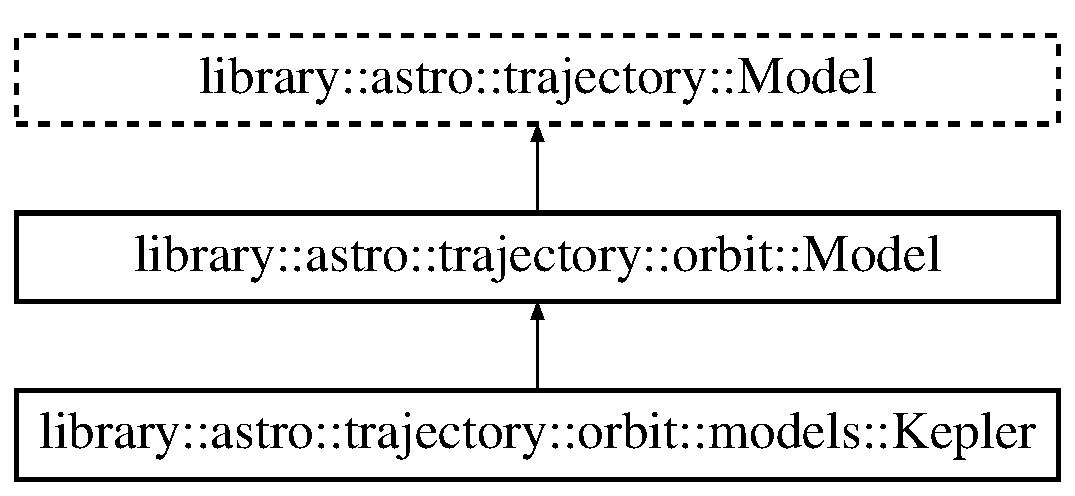
\includegraphics[height=3.000000cm]{classlibrary_1_1astro_1_1trajectory_1_1orbit_1_1models_1_1_kepler}
\end{center}
\end{figure}
\subsection*{Public Types}
\begin{DoxyCompactItemize}
\item 
enum \hyperlink{classlibrary_1_1astro_1_1trajectory_1_1orbit_1_1models_1_1_kepler_a7f34995d6f287de65a6edb2d419a2fe0}{Perturbation\+Type} \{ \hyperlink{classlibrary_1_1astro_1_1trajectory_1_1orbit_1_1models_1_1_kepler_a7f34995d6f287de65a6edb2d419a2fe0a6adf97f83acf6453d4a6a4b1070f3754}{Perturbation\+Type\+::\+None}, 
\hyperlink{classlibrary_1_1astro_1_1trajectory_1_1orbit_1_1models_1_1_kepler_a7f34995d6f287de65a6edb2d419a2fe0a7f132d501fb9863844ab51697900d494}{Perturbation\+Type\+::\+J2}
 \}
\end{DoxyCompactItemize}
\subsection*{Public Member Functions}
\begin{DoxyCompactItemize}
\item 
\hyperlink{classlibrary_1_1astro_1_1trajectory_1_1orbit_1_1models_1_1_kepler_ae0c322251dbb025bfbdefd9f7b97e018}{Kepler} (const \hyperlink{classlibrary_1_1astro_1_1trajectory_1_1orbit_1_1models_1_1kepler_1_1_c_o_e}{C\+OE} \&a\+Classical\+Orbital\+Element\+Set, const Instant \&an\+Epoch, const Derived \&a\+Gravitational\+Parameter, const Length \&an\+Equatorial\+Radius, const Real \&a\+J2, const \hyperlink{classlibrary_1_1astro_1_1trajectory_1_1orbit_1_1models_1_1_kepler_a7f34995d6f287de65a6edb2d419a2fe0}{Kepler\+::\+Perturbation\+Type} \&a\+Perturbation\+Type)
\item 
\hyperlink{classlibrary_1_1astro_1_1trajectory_1_1orbit_1_1models_1_1_kepler_a07fe8f18505ab866ba777fc37e8390a3}{Kepler} (const \hyperlink{classlibrary_1_1astro_1_1trajectory_1_1orbit_1_1models_1_1kepler_1_1_c_o_e}{C\+OE} \&a\+Classical\+Orbital\+Element\+Set, const Instant \&an\+Epoch, const Celestial \&a\+Celestial\+Object, const \hyperlink{classlibrary_1_1astro_1_1trajectory_1_1orbit_1_1models_1_1_kepler_a7f34995d6f287de65a6edb2d419a2fe0}{Kepler\+::\+Perturbation\+Type} \&a\+Perturbation\+Type, const bool in\+Fixed\+Frame=false)
\item 
virtual \hyperlink{classlibrary_1_1astro_1_1trajectory_1_1orbit_1_1models_1_1_kepler}{Kepler} $\ast$ \hyperlink{classlibrary_1_1astro_1_1trajectory_1_1orbit_1_1models_1_1_kepler_ac78a023cde4a61c62309051c9147d66e}{clone} () const override
\item 
bool \hyperlink{classlibrary_1_1astro_1_1trajectory_1_1orbit_1_1models_1_1_kepler_a1fbf0650ece0aa4fd99bc9d8d4bc1f77}{operator==} (const \hyperlink{classlibrary_1_1astro_1_1trajectory_1_1orbit_1_1models_1_1_kepler}{Kepler} \&a\+Keplerian\+Model) const
\item 
bool \hyperlink{classlibrary_1_1astro_1_1trajectory_1_1orbit_1_1models_1_1_kepler_a38a315b4ffbfe6293c2570ade157865c}{operator!=} (const \hyperlink{classlibrary_1_1astro_1_1trajectory_1_1orbit_1_1models_1_1_kepler}{Kepler} \&a\+Keplerian\+Model) const
\item 
virtual bool \hyperlink{classlibrary_1_1astro_1_1trajectory_1_1orbit_1_1models_1_1_kepler_a600d7752a50924ee6e3fc08f18a229e9}{is\+Defined} () const override
\item 
\hyperlink{classlibrary_1_1astro_1_1trajectory_1_1orbit_1_1models_1_1kepler_1_1_c_o_e}{C\+OE} \hyperlink{classlibrary_1_1astro_1_1trajectory_1_1orbit_1_1models_1_1_kepler_a224a8ad539b7739447a0e9bd98e6f66d}{get\+Classical\+Orbital\+Elements} () const
\item 
virtual Instant \hyperlink{classlibrary_1_1astro_1_1trajectory_1_1orbit_1_1models_1_1_kepler_a6ecdd4a133cdd936909020b644dd8f1f}{get\+Epoch} () const override
\item 
virtual Integer \hyperlink{classlibrary_1_1astro_1_1trajectory_1_1orbit_1_1models_1_1_kepler_ad8df985c06ca56c1516f3b8804d5052d}{get\+Revolution\+Number\+At\+Epoch} () const override
\item 
Derived \hyperlink{classlibrary_1_1astro_1_1trajectory_1_1orbit_1_1models_1_1_kepler_a65ba42289312a4d54adfbf14589d8dde}{get\+Gravitational\+Parameter} () const
\item 
Length \hyperlink{classlibrary_1_1astro_1_1trajectory_1_1orbit_1_1models_1_1_kepler_a687374bb06a2f805a21ded57f2604c4b}{get\+Equatorial\+Radius} () const
\item 
Real \hyperlink{classlibrary_1_1astro_1_1trajectory_1_1orbit_1_1models_1_1_kepler_ab6a582f7b6ab6f9f22e180378e20b58d}{get\+J2} () const
\item 
\hyperlink{classlibrary_1_1astro_1_1trajectory_1_1orbit_1_1models_1_1_kepler_a7f34995d6f287de65a6edb2d419a2fe0}{Kepler\+::\+Perturbation\+Type} \hyperlink{classlibrary_1_1astro_1_1trajectory_1_1orbit_1_1models_1_1_kepler_a68033efefbad3ba3d52558cecd606820}{get\+Perturbation\+Type} () const
\item 
virtual \hyperlink{classlibrary_1_1astro_1_1trajectory_1_1_state}{State} \hyperlink{classlibrary_1_1astro_1_1trajectory_1_1orbit_1_1models_1_1_kepler_a6354b3545decf1179289383679ebe2cd}{calculate\+State\+At} (const Instant \&an\+Instant) const override
\item 
virtual Integer \hyperlink{classlibrary_1_1astro_1_1trajectory_1_1orbit_1_1models_1_1_kepler_a9ba435e737c10933f39d4817306810eb}{calculate\+Revolution\+Number\+At} (const Instant \&an\+Instant) const override
\item 
virtual void \hyperlink{classlibrary_1_1astro_1_1trajectory_1_1orbit_1_1models_1_1_kepler_a5cecedfe1b2002881b4ef6eeae64af93}{print} (std\+::ostream \&an\+Output\+Stream, bool display\+Decorator=true) const override
\end{DoxyCompactItemize}
\subsection*{Static Public Member Functions}
\begin{DoxyCompactItemize}
\item 
static String \hyperlink{classlibrary_1_1astro_1_1trajectory_1_1orbit_1_1models_1_1_kepler_a0ab0792e822cf9586d55fa17e3950d87}{String\+From\+Perturbation\+Type} (const \hyperlink{classlibrary_1_1astro_1_1trajectory_1_1orbit_1_1models_1_1_kepler_a7f34995d6f287de65a6edb2d419a2fe0}{Kepler\+::\+Perturbation\+Type} \&a\+Perturbation\+Type)
\end{DoxyCompactItemize}
\subsection*{Protected Member Functions}
\begin{DoxyCompactItemize}
\item 
virtual bool \hyperlink{classlibrary_1_1astro_1_1trajectory_1_1orbit_1_1models_1_1_kepler_af3adc1e4bee0a3064963209b58178e98}{operator==} (const \hyperlink{classlibrary_1_1astro_1_1trajectory_1_1_model}{trajectory\+::\+Model} \&a\+Model) const override
\item 
virtual bool \hyperlink{classlibrary_1_1astro_1_1trajectory_1_1orbit_1_1models_1_1_kepler_a2671d995d476b11a14cc08aad2dc0b30}{operator!=} (const \hyperlink{classlibrary_1_1astro_1_1trajectory_1_1_model}{trajectory\+::\+Model} \&a\+Model) const override
\end{DoxyCompactItemize}
\subsection*{Friends}
\begin{DoxyCompactItemize}
\item 
std\+::ostream \& \hyperlink{classlibrary_1_1astro_1_1trajectory_1_1orbit_1_1models_1_1_kepler_aedb386ce32716dfb187f89b52b023f2b}{operator$<$$<$} (std\+::ostream \&an\+Output\+Stream, const \hyperlink{classlibrary_1_1astro_1_1trajectory_1_1orbit_1_1models_1_1_kepler}{Kepler} \&a\+Keplerian\+Model)
\end{DoxyCompactItemize}


\subsection{Member Enumeration Documentation}
\mbox{\Hypertarget{classlibrary_1_1astro_1_1trajectory_1_1orbit_1_1models_1_1_kepler_a7f34995d6f287de65a6edb2d419a2fe0}\label{classlibrary_1_1astro_1_1trajectory_1_1orbit_1_1models_1_1_kepler_a7f34995d6f287de65a6edb2d419a2fe0}} 
\index{library\+::astro\+::trajectory\+::orbit\+::models\+::\+Kepler@{library\+::astro\+::trajectory\+::orbit\+::models\+::\+Kepler}!Perturbation\+Type@{Perturbation\+Type}}
\index{Perturbation\+Type@{Perturbation\+Type}!library\+::astro\+::trajectory\+::orbit\+::models\+::\+Kepler@{library\+::astro\+::trajectory\+::orbit\+::models\+::\+Kepler}}
\subsubsection{\texorpdfstring{Perturbation\+Type}{PerturbationType}}
{\footnotesize\ttfamily enum \hyperlink{classlibrary_1_1astro_1_1trajectory_1_1orbit_1_1models_1_1_kepler_a7f34995d6f287de65a6edb2d419a2fe0}{library\+::astro\+::trajectory\+::orbit\+::models\+::\+Kepler\+::\+Perturbation\+Type}\hspace{0.3cm}{\ttfamily [strong]}}

\begin{DoxyEnumFields}{Enumerator}
\raisebox{\heightof{T}}[0pt][0pt]{\index{None@{None}!library\+::astro\+::trajectory\+::orbit\+::models\+::\+Kepler@{library\+::astro\+::trajectory\+::orbit\+::models\+::\+Kepler}}\index{library\+::astro\+::trajectory\+::orbit\+::models\+::\+Kepler@{library\+::astro\+::trajectory\+::orbit\+::models\+::\+Kepler}!None@{None}}}\mbox{\Hypertarget{classlibrary_1_1astro_1_1trajectory_1_1orbit_1_1models_1_1_kepler_a7f34995d6f287de65a6edb2d419a2fe0a6adf97f83acf6453d4a6a4b1070f3754}\label{classlibrary_1_1astro_1_1trajectory_1_1orbit_1_1models_1_1_kepler_a7f34995d6f287de65a6edb2d419a2fe0a6adf97f83acf6453d4a6a4b1070f3754}} 
None&\\
\hline

\raisebox{\heightof{T}}[0pt][0pt]{\index{J2@{J2}!library\+::astro\+::trajectory\+::orbit\+::models\+::\+Kepler@{library\+::astro\+::trajectory\+::orbit\+::models\+::\+Kepler}}\index{library\+::astro\+::trajectory\+::orbit\+::models\+::\+Kepler@{library\+::astro\+::trajectory\+::orbit\+::models\+::\+Kepler}!J2@{J2}}}\mbox{\Hypertarget{classlibrary_1_1astro_1_1trajectory_1_1orbit_1_1models_1_1_kepler_a7f34995d6f287de65a6edb2d419a2fe0a7f132d501fb9863844ab51697900d494}\label{classlibrary_1_1astro_1_1trajectory_1_1orbit_1_1models_1_1_kepler_a7f34995d6f287de65a6edb2d419a2fe0a7f132d501fb9863844ab51697900d494}} 
J2&\\
\hline

\end{DoxyEnumFields}


\subsection{Constructor \& Destructor Documentation}
\mbox{\Hypertarget{classlibrary_1_1astro_1_1trajectory_1_1orbit_1_1models_1_1_kepler_ae0c322251dbb025bfbdefd9f7b97e018}\label{classlibrary_1_1astro_1_1trajectory_1_1orbit_1_1models_1_1_kepler_ae0c322251dbb025bfbdefd9f7b97e018}} 
\index{library\+::astro\+::trajectory\+::orbit\+::models\+::\+Kepler@{library\+::astro\+::trajectory\+::orbit\+::models\+::\+Kepler}!Kepler@{Kepler}}
\index{Kepler@{Kepler}!library\+::astro\+::trajectory\+::orbit\+::models\+::\+Kepler@{library\+::astro\+::trajectory\+::orbit\+::models\+::\+Kepler}}
\subsubsection{\texorpdfstring{Kepler()}{Kepler()}\hspace{0.1cm}{\footnotesize\ttfamily [1/2]}}
{\footnotesize\ttfamily library\+::astro\+::trajectory\+::orbit\+::models\+::\+Kepler\+::\+Kepler (\begin{DoxyParamCaption}\item[{const \hyperlink{classlibrary_1_1astro_1_1trajectory_1_1orbit_1_1models_1_1kepler_1_1_c_o_e}{C\+OE} \&}]{a\+Classical\+Orbital\+Element\+Set,  }\item[{const Instant \&}]{an\+Epoch,  }\item[{const Derived \&}]{a\+Gravitational\+Parameter,  }\item[{const Length \&}]{an\+Equatorial\+Radius,  }\item[{const Real \&}]{a\+J2,  }\item[{const \hyperlink{classlibrary_1_1astro_1_1trajectory_1_1orbit_1_1models_1_1_kepler_a7f34995d6f287de65a6edb2d419a2fe0}{Kepler\+::\+Perturbation\+Type} \&}]{a\+Perturbation\+Type }\end{DoxyParamCaption})}

\mbox{\Hypertarget{classlibrary_1_1astro_1_1trajectory_1_1orbit_1_1models_1_1_kepler_a07fe8f18505ab866ba777fc37e8390a3}\label{classlibrary_1_1astro_1_1trajectory_1_1orbit_1_1models_1_1_kepler_a07fe8f18505ab866ba777fc37e8390a3}} 
\index{library\+::astro\+::trajectory\+::orbit\+::models\+::\+Kepler@{library\+::astro\+::trajectory\+::orbit\+::models\+::\+Kepler}!Kepler@{Kepler}}
\index{Kepler@{Kepler}!library\+::astro\+::trajectory\+::orbit\+::models\+::\+Kepler@{library\+::astro\+::trajectory\+::orbit\+::models\+::\+Kepler}}
\subsubsection{\texorpdfstring{Kepler()}{Kepler()}\hspace{0.1cm}{\footnotesize\ttfamily [2/2]}}
{\footnotesize\ttfamily library\+::astro\+::trajectory\+::orbit\+::models\+::\+Kepler\+::\+Kepler (\begin{DoxyParamCaption}\item[{const \hyperlink{classlibrary_1_1astro_1_1trajectory_1_1orbit_1_1models_1_1kepler_1_1_c_o_e}{C\+OE} \&}]{a\+Classical\+Orbital\+Element\+Set,  }\item[{const Instant \&}]{an\+Epoch,  }\item[{const Celestial \&}]{a\+Celestial\+Object,  }\item[{const \hyperlink{classlibrary_1_1astro_1_1trajectory_1_1orbit_1_1models_1_1_kepler_a7f34995d6f287de65a6edb2d419a2fe0}{Kepler\+::\+Perturbation\+Type} \&}]{a\+Perturbation\+Type,  }\item[{const bool}]{in\+Fixed\+Frame = {\ttfamily false} }\end{DoxyParamCaption})}



\subsection{Member Function Documentation}
\mbox{\Hypertarget{classlibrary_1_1astro_1_1trajectory_1_1orbit_1_1models_1_1_kepler_a9ba435e737c10933f39d4817306810eb}\label{classlibrary_1_1astro_1_1trajectory_1_1orbit_1_1models_1_1_kepler_a9ba435e737c10933f39d4817306810eb}} 
\index{library\+::astro\+::trajectory\+::orbit\+::models\+::\+Kepler@{library\+::astro\+::trajectory\+::orbit\+::models\+::\+Kepler}!calculate\+Revolution\+Number\+At@{calculate\+Revolution\+Number\+At}}
\index{calculate\+Revolution\+Number\+At@{calculate\+Revolution\+Number\+At}!library\+::astro\+::trajectory\+::orbit\+::models\+::\+Kepler@{library\+::astro\+::trajectory\+::orbit\+::models\+::\+Kepler}}
\subsubsection{\texorpdfstring{calculate\+Revolution\+Number\+At()}{calculateRevolutionNumberAt()}}
{\footnotesize\ttfamily Integer library\+::astro\+::trajectory\+::orbit\+::models\+::\+Kepler\+::calculate\+Revolution\+Number\+At (\begin{DoxyParamCaption}\item[{const Instant \&}]{an\+Instant }\end{DoxyParamCaption}) const\hspace{0.3cm}{\ttfamily [override]}, {\ttfamily [virtual]}}



Implements \hyperlink{classlibrary_1_1astro_1_1trajectory_1_1orbit_1_1_model_a6329db5556ed72aa8ad18515aeaefeab}{library\+::astro\+::trajectory\+::orbit\+::\+Model}.

\mbox{\Hypertarget{classlibrary_1_1astro_1_1trajectory_1_1orbit_1_1models_1_1_kepler_a6354b3545decf1179289383679ebe2cd}\label{classlibrary_1_1astro_1_1trajectory_1_1orbit_1_1models_1_1_kepler_a6354b3545decf1179289383679ebe2cd}} 
\index{library\+::astro\+::trajectory\+::orbit\+::models\+::\+Kepler@{library\+::astro\+::trajectory\+::orbit\+::models\+::\+Kepler}!calculate\+State\+At@{calculate\+State\+At}}
\index{calculate\+State\+At@{calculate\+State\+At}!library\+::astro\+::trajectory\+::orbit\+::models\+::\+Kepler@{library\+::astro\+::trajectory\+::orbit\+::models\+::\+Kepler}}
\subsubsection{\texorpdfstring{calculate\+State\+At()}{calculateStateAt()}}
{\footnotesize\ttfamily \hyperlink{classlibrary_1_1astro_1_1trajectory_1_1_state}{State} library\+::astro\+::trajectory\+::orbit\+::models\+::\+Kepler\+::calculate\+State\+At (\begin{DoxyParamCaption}\item[{const Instant \&}]{an\+Instant }\end{DoxyParamCaption}) const\hspace{0.3cm}{\ttfamily [override]}, {\ttfamily [virtual]}}



Implements \hyperlink{classlibrary_1_1astro_1_1trajectory_1_1orbit_1_1_model_a34198a504836b9779425da99d964d19c}{library\+::astro\+::trajectory\+::orbit\+::\+Model}.

\mbox{\Hypertarget{classlibrary_1_1astro_1_1trajectory_1_1orbit_1_1models_1_1_kepler_ac78a023cde4a61c62309051c9147d66e}\label{classlibrary_1_1astro_1_1trajectory_1_1orbit_1_1models_1_1_kepler_ac78a023cde4a61c62309051c9147d66e}} 
\index{library\+::astro\+::trajectory\+::orbit\+::models\+::\+Kepler@{library\+::astro\+::trajectory\+::orbit\+::models\+::\+Kepler}!clone@{clone}}
\index{clone@{clone}!library\+::astro\+::trajectory\+::orbit\+::models\+::\+Kepler@{library\+::astro\+::trajectory\+::orbit\+::models\+::\+Kepler}}
\subsubsection{\texorpdfstring{clone()}{clone()}}
{\footnotesize\ttfamily \hyperlink{classlibrary_1_1astro_1_1trajectory_1_1orbit_1_1models_1_1_kepler}{Kepler} $\ast$ library\+::astro\+::trajectory\+::orbit\+::models\+::\+Kepler\+::clone (\begin{DoxyParamCaption}{ }\end{DoxyParamCaption}) const\hspace{0.3cm}{\ttfamily [override]}, {\ttfamily [virtual]}}



Implements \hyperlink{classlibrary_1_1astro_1_1trajectory_1_1orbit_1_1_model_a45d75e4d212a9bb01aa596eaeeae43ae}{library\+::astro\+::trajectory\+::orbit\+::\+Model}.

\mbox{\Hypertarget{classlibrary_1_1astro_1_1trajectory_1_1orbit_1_1models_1_1_kepler_a224a8ad539b7739447a0e9bd98e6f66d}\label{classlibrary_1_1astro_1_1trajectory_1_1orbit_1_1models_1_1_kepler_a224a8ad539b7739447a0e9bd98e6f66d}} 
\index{library\+::astro\+::trajectory\+::orbit\+::models\+::\+Kepler@{library\+::astro\+::trajectory\+::orbit\+::models\+::\+Kepler}!get\+Classical\+Orbital\+Elements@{get\+Classical\+Orbital\+Elements}}
\index{get\+Classical\+Orbital\+Elements@{get\+Classical\+Orbital\+Elements}!library\+::astro\+::trajectory\+::orbit\+::models\+::\+Kepler@{library\+::astro\+::trajectory\+::orbit\+::models\+::\+Kepler}}
\subsubsection{\texorpdfstring{get\+Classical\+Orbital\+Elements()}{getClassicalOrbitalElements()}}
{\footnotesize\ttfamily \hyperlink{classlibrary_1_1astro_1_1trajectory_1_1orbit_1_1models_1_1kepler_1_1_c_o_e}{C\+OE} library\+::astro\+::trajectory\+::orbit\+::models\+::\+Kepler\+::get\+Classical\+Orbital\+Elements (\begin{DoxyParamCaption}{ }\end{DoxyParamCaption}) const}

\mbox{\Hypertarget{classlibrary_1_1astro_1_1trajectory_1_1orbit_1_1models_1_1_kepler_a6ecdd4a133cdd936909020b644dd8f1f}\label{classlibrary_1_1astro_1_1trajectory_1_1orbit_1_1models_1_1_kepler_a6ecdd4a133cdd936909020b644dd8f1f}} 
\index{library\+::astro\+::trajectory\+::orbit\+::models\+::\+Kepler@{library\+::astro\+::trajectory\+::orbit\+::models\+::\+Kepler}!get\+Epoch@{get\+Epoch}}
\index{get\+Epoch@{get\+Epoch}!library\+::astro\+::trajectory\+::orbit\+::models\+::\+Kepler@{library\+::astro\+::trajectory\+::orbit\+::models\+::\+Kepler}}
\subsubsection{\texorpdfstring{get\+Epoch()}{getEpoch()}}
{\footnotesize\ttfamily Instant library\+::astro\+::trajectory\+::orbit\+::models\+::\+Kepler\+::get\+Epoch (\begin{DoxyParamCaption}{ }\end{DoxyParamCaption}) const\hspace{0.3cm}{\ttfamily [override]}, {\ttfamily [virtual]}}



Implements \hyperlink{classlibrary_1_1astro_1_1trajectory_1_1orbit_1_1_model_acdec7ed6eed001c2ab4ac5442699a316}{library\+::astro\+::trajectory\+::orbit\+::\+Model}.

\mbox{\Hypertarget{classlibrary_1_1astro_1_1trajectory_1_1orbit_1_1models_1_1_kepler_a687374bb06a2f805a21ded57f2604c4b}\label{classlibrary_1_1astro_1_1trajectory_1_1orbit_1_1models_1_1_kepler_a687374bb06a2f805a21ded57f2604c4b}} 
\index{library\+::astro\+::trajectory\+::orbit\+::models\+::\+Kepler@{library\+::astro\+::trajectory\+::orbit\+::models\+::\+Kepler}!get\+Equatorial\+Radius@{get\+Equatorial\+Radius}}
\index{get\+Equatorial\+Radius@{get\+Equatorial\+Radius}!library\+::astro\+::trajectory\+::orbit\+::models\+::\+Kepler@{library\+::astro\+::trajectory\+::orbit\+::models\+::\+Kepler}}
\subsubsection{\texorpdfstring{get\+Equatorial\+Radius()}{getEquatorialRadius()}}
{\footnotesize\ttfamily Length library\+::astro\+::trajectory\+::orbit\+::models\+::\+Kepler\+::get\+Equatorial\+Radius (\begin{DoxyParamCaption}{ }\end{DoxyParamCaption}) const}

\mbox{\Hypertarget{classlibrary_1_1astro_1_1trajectory_1_1orbit_1_1models_1_1_kepler_a65ba42289312a4d54adfbf14589d8dde}\label{classlibrary_1_1astro_1_1trajectory_1_1orbit_1_1models_1_1_kepler_a65ba42289312a4d54adfbf14589d8dde}} 
\index{library\+::astro\+::trajectory\+::orbit\+::models\+::\+Kepler@{library\+::astro\+::trajectory\+::orbit\+::models\+::\+Kepler}!get\+Gravitational\+Parameter@{get\+Gravitational\+Parameter}}
\index{get\+Gravitational\+Parameter@{get\+Gravitational\+Parameter}!library\+::astro\+::trajectory\+::orbit\+::models\+::\+Kepler@{library\+::astro\+::trajectory\+::orbit\+::models\+::\+Kepler}}
\subsubsection{\texorpdfstring{get\+Gravitational\+Parameter()}{getGravitationalParameter()}}
{\footnotesize\ttfamily Derived library\+::astro\+::trajectory\+::orbit\+::models\+::\+Kepler\+::get\+Gravitational\+Parameter (\begin{DoxyParamCaption}{ }\end{DoxyParamCaption}) const}

\mbox{\Hypertarget{classlibrary_1_1astro_1_1trajectory_1_1orbit_1_1models_1_1_kepler_ab6a582f7b6ab6f9f22e180378e20b58d}\label{classlibrary_1_1astro_1_1trajectory_1_1orbit_1_1models_1_1_kepler_ab6a582f7b6ab6f9f22e180378e20b58d}} 
\index{library\+::astro\+::trajectory\+::orbit\+::models\+::\+Kepler@{library\+::astro\+::trajectory\+::orbit\+::models\+::\+Kepler}!get\+J2@{get\+J2}}
\index{get\+J2@{get\+J2}!library\+::astro\+::trajectory\+::orbit\+::models\+::\+Kepler@{library\+::astro\+::trajectory\+::orbit\+::models\+::\+Kepler}}
\subsubsection{\texorpdfstring{get\+J2()}{getJ2()}}
{\footnotesize\ttfamily Real library\+::astro\+::trajectory\+::orbit\+::models\+::\+Kepler\+::get\+J2 (\begin{DoxyParamCaption}{ }\end{DoxyParamCaption}) const}

\mbox{\Hypertarget{classlibrary_1_1astro_1_1trajectory_1_1orbit_1_1models_1_1_kepler_a68033efefbad3ba3d52558cecd606820}\label{classlibrary_1_1astro_1_1trajectory_1_1orbit_1_1models_1_1_kepler_a68033efefbad3ba3d52558cecd606820}} 
\index{library\+::astro\+::trajectory\+::orbit\+::models\+::\+Kepler@{library\+::astro\+::trajectory\+::orbit\+::models\+::\+Kepler}!get\+Perturbation\+Type@{get\+Perturbation\+Type}}
\index{get\+Perturbation\+Type@{get\+Perturbation\+Type}!library\+::astro\+::trajectory\+::orbit\+::models\+::\+Kepler@{library\+::astro\+::trajectory\+::orbit\+::models\+::\+Kepler}}
\subsubsection{\texorpdfstring{get\+Perturbation\+Type()}{getPerturbationType()}}
{\footnotesize\ttfamily \hyperlink{classlibrary_1_1astro_1_1trajectory_1_1orbit_1_1models_1_1_kepler_a7f34995d6f287de65a6edb2d419a2fe0}{Kepler\+::\+Perturbation\+Type} library\+::astro\+::trajectory\+::orbit\+::models\+::\+Kepler\+::get\+Perturbation\+Type (\begin{DoxyParamCaption}{ }\end{DoxyParamCaption}) const}

\mbox{\Hypertarget{classlibrary_1_1astro_1_1trajectory_1_1orbit_1_1models_1_1_kepler_ad8df985c06ca56c1516f3b8804d5052d}\label{classlibrary_1_1astro_1_1trajectory_1_1orbit_1_1models_1_1_kepler_ad8df985c06ca56c1516f3b8804d5052d}} 
\index{library\+::astro\+::trajectory\+::orbit\+::models\+::\+Kepler@{library\+::astro\+::trajectory\+::orbit\+::models\+::\+Kepler}!get\+Revolution\+Number\+At\+Epoch@{get\+Revolution\+Number\+At\+Epoch}}
\index{get\+Revolution\+Number\+At\+Epoch@{get\+Revolution\+Number\+At\+Epoch}!library\+::astro\+::trajectory\+::orbit\+::models\+::\+Kepler@{library\+::astro\+::trajectory\+::orbit\+::models\+::\+Kepler}}
\subsubsection{\texorpdfstring{get\+Revolution\+Number\+At\+Epoch()}{getRevolutionNumberAtEpoch()}}
{\footnotesize\ttfamily Integer library\+::astro\+::trajectory\+::orbit\+::models\+::\+Kepler\+::get\+Revolution\+Number\+At\+Epoch (\begin{DoxyParamCaption}{ }\end{DoxyParamCaption}) const\hspace{0.3cm}{\ttfamily [override]}, {\ttfamily [virtual]}}



Implements \hyperlink{classlibrary_1_1astro_1_1trajectory_1_1orbit_1_1_model_a940f5e266feb90ee8264d4c7a8a883f3}{library\+::astro\+::trajectory\+::orbit\+::\+Model}.

\mbox{\Hypertarget{classlibrary_1_1astro_1_1trajectory_1_1orbit_1_1models_1_1_kepler_a600d7752a50924ee6e3fc08f18a229e9}\label{classlibrary_1_1astro_1_1trajectory_1_1orbit_1_1models_1_1_kepler_a600d7752a50924ee6e3fc08f18a229e9}} 
\index{library\+::astro\+::trajectory\+::orbit\+::models\+::\+Kepler@{library\+::astro\+::trajectory\+::orbit\+::models\+::\+Kepler}!is\+Defined@{is\+Defined}}
\index{is\+Defined@{is\+Defined}!library\+::astro\+::trajectory\+::orbit\+::models\+::\+Kepler@{library\+::astro\+::trajectory\+::orbit\+::models\+::\+Kepler}}
\subsubsection{\texorpdfstring{is\+Defined()}{isDefined()}}
{\footnotesize\ttfamily bool library\+::astro\+::trajectory\+::orbit\+::models\+::\+Kepler\+::is\+Defined (\begin{DoxyParamCaption}{ }\end{DoxyParamCaption}) const\hspace{0.3cm}{\ttfamily [override]}, {\ttfamily [virtual]}}



Implements \hyperlink{classlibrary_1_1astro_1_1trajectory_1_1orbit_1_1_model_a518785603421d259e427bd0a6ee5e787}{library\+::astro\+::trajectory\+::orbit\+::\+Model}.

\mbox{\Hypertarget{classlibrary_1_1astro_1_1trajectory_1_1orbit_1_1models_1_1_kepler_a38a315b4ffbfe6293c2570ade157865c}\label{classlibrary_1_1astro_1_1trajectory_1_1orbit_1_1models_1_1_kepler_a38a315b4ffbfe6293c2570ade157865c}} 
\index{library\+::astro\+::trajectory\+::orbit\+::models\+::\+Kepler@{library\+::astro\+::trajectory\+::orbit\+::models\+::\+Kepler}!operator"!=@{operator"!=}}
\index{operator"!=@{operator"!=}!library\+::astro\+::trajectory\+::orbit\+::models\+::\+Kepler@{library\+::astro\+::trajectory\+::orbit\+::models\+::\+Kepler}}
\subsubsection{\texorpdfstring{operator"!=()}{operator!=()}\hspace{0.1cm}{\footnotesize\ttfamily [1/2]}}
{\footnotesize\ttfamily bool library\+::astro\+::trajectory\+::orbit\+::models\+::\+Kepler\+::operator!= (\begin{DoxyParamCaption}\item[{const \hyperlink{classlibrary_1_1astro_1_1trajectory_1_1orbit_1_1models_1_1_kepler}{Kepler} \&}]{a\+Keplerian\+Model }\end{DoxyParamCaption}) const}

\mbox{\Hypertarget{classlibrary_1_1astro_1_1trajectory_1_1orbit_1_1models_1_1_kepler_a2671d995d476b11a14cc08aad2dc0b30}\label{classlibrary_1_1astro_1_1trajectory_1_1orbit_1_1models_1_1_kepler_a2671d995d476b11a14cc08aad2dc0b30}} 
\index{library\+::astro\+::trajectory\+::orbit\+::models\+::\+Kepler@{library\+::astro\+::trajectory\+::orbit\+::models\+::\+Kepler}!operator"!=@{operator"!=}}
\index{operator"!=@{operator"!=}!library\+::astro\+::trajectory\+::orbit\+::models\+::\+Kepler@{library\+::astro\+::trajectory\+::orbit\+::models\+::\+Kepler}}
\subsubsection{\texorpdfstring{operator"!=()}{operator!=()}\hspace{0.1cm}{\footnotesize\ttfamily [2/2]}}
{\footnotesize\ttfamily bool library\+::astro\+::trajectory\+::orbit\+::models\+::\+Kepler\+::operator!= (\begin{DoxyParamCaption}\item[{const \hyperlink{classlibrary_1_1astro_1_1trajectory_1_1_model}{trajectory\+::\+Model} \&}]{a\+Model }\end{DoxyParamCaption}) const\hspace{0.3cm}{\ttfamily [override]}, {\ttfamily [protected]}, {\ttfamily [virtual]}}



Implements \hyperlink{classlibrary_1_1astro_1_1trajectory_1_1_model_a476c234f5fca1eb75f64f5a96fd83c61}{library\+::astro\+::trajectory\+::\+Model}.

\mbox{\Hypertarget{classlibrary_1_1astro_1_1trajectory_1_1orbit_1_1models_1_1_kepler_a1fbf0650ece0aa4fd99bc9d8d4bc1f77}\label{classlibrary_1_1astro_1_1trajectory_1_1orbit_1_1models_1_1_kepler_a1fbf0650ece0aa4fd99bc9d8d4bc1f77}} 
\index{library\+::astro\+::trajectory\+::orbit\+::models\+::\+Kepler@{library\+::astro\+::trajectory\+::orbit\+::models\+::\+Kepler}!operator==@{operator==}}
\index{operator==@{operator==}!library\+::astro\+::trajectory\+::orbit\+::models\+::\+Kepler@{library\+::astro\+::trajectory\+::orbit\+::models\+::\+Kepler}}
\subsubsection{\texorpdfstring{operator==()}{operator==()}\hspace{0.1cm}{\footnotesize\ttfamily [1/2]}}
{\footnotesize\ttfamily bool library\+::astro\+::trajectory\+::orbit\+::models\+::\+Kepler\+::operator== (\begin{DoxyParamCaption}\item[{const \hyperlink{classlibrary_1_1astro_1_1trajectory_1_1orbit_1_1models_1_1_kepler}{Kepler} \&}]{a\+Keplerian\+Model }\end{DoxyParamCaption}) const}

\mbox{\Hypertarget{classlibrary_1_1astro_1_1trajectory_1_1orbit_1_1models_1_1_kepler_af3adc1e4bee0a3064963209b58178e98}\label{classlibrary_1_1astro_1_1trajectory_1_1orbit_1_1models_1_1_kepler_af3adc1e4bee0a3064963209b58178e98}} 
\index{library\+::astro\+::trajectory\+::orbit\+::models\+::\+Kepler@{library\+::astro\+::trajectory\+::orbit\+::models\+::\+Kepler}!operator==@{operator==}}
\index{operator==@{operator==}!library\+::astro\+::trajectory\+::orbit\+::models\+::\+Kepler@{library\+::astro\+::trajectory\+::orbit\+::models\+::\+Kepler}}
\subsubsection{\texorpdfstring{operator==()}{operator==()}\hspace{0.1cm}{\footnotesize\ttfamily [2/2]}}
{\footnotesize\ttfamily bool library\+::astro\+::trajectory\+::orbit\+::models\+::\+Kepler\+::operator== (\begin{DoxyParamCaption}\item[{const \hyperlink{classlibrary_1_1astro_1_1trajectory_1_1_model}{trajectory\+::\+Model} \&}]{a\+Model }\end{DoxyParamCaption}) const\hspace{0.3cm}{\ttfamily [override]}, {\ttfamily [protected]}, {\ttfamily [virtual]}}



Implements \hyperlink{classlibrary_1_1astro_1_1trajectory_1_1_model_a83c52eb23e8feea58d600c87700ed923}{library\+::astro\+::trajectory\+::\+Model}.

\mbox{\Hypertarget{classlibrary_1_1astro_1_1trajectory_1_1orbit_1_1models_1_1_kepler_a5cecedfe1b2002881b4ef6eeae64af93}\label{classlibrary_1_1astro_1_1trajectory_1_1orbit_1_1models_1_1_kepler_a5cecedfe1b2002881b4ef6eeae64af93}} 
\index{library\+::astro\+::trajectory\+::orbit\+::models\+::\+Kepler@{library\+::astro\+::trajectory\+::orbit\+::models\+::\+Kepler}!print@{print}}
\index{print@{print}!library\+::astro\+::trajectory\+::orbit\+::models\+::\+Kepler@{library\+::astro\+::trajectory\+::orbit\+::models\+::\+Kepler}}
\subsubsection{\texorpdfstring{print()}{print()}}
{\footnotesize\ttfamily void library\+::astro\+::trajectory\+::orbit\+::models\+::\+Kepler\+::print (\begin{DoxyParamCaption}\item[{std\+::ostream \&}]{an\+Output\+Stream,  }\item[{bool}]{display\+Decorator = {\ttfamily true} }\end{DoxyParamCaption}) const\hspace{0.3cm}{\ttfamily [override]}, {\ttfamily [virtual]}}



Implements \hyperlink{classlibrary_1_1astro_1_1trajectory_1_1orbit_1_1_model_abd4fb7604274cc8b3589a445db64e98c}{library\+::astro\+::trajectory\+::orbit\+::\+Model}.

\mbox{\Hypertarget{classlibrary_1_1astro_1_1trajectory_1_1orbit_1_1models_1_1_kepler_a0ab0792e822cf9586d55fa17e3950d87}\label{classlibrary_1_1astro_1_1trajectory_1_1orbit_1_1models_1_1_kepler_a0ab0792e822cf9586d55fa17e3950d87}} 
\index{library\+::astro\+::trajectory\+::orbit\+::models\+::\+Kepler@{library\+::astro\+::trajectory\+::orbit\+::models\+::\+Kepler}!String\+From\+Perturbation\+Type@{String\+From\+Perturbation\+Type}}
\index{String\+From\+Perturbation\+Type@{String\+From\+Perturbation\+Type}!library\+::astro\+::trajectory\+::orbit\+::models\+::\+Kepler@{library\+::astro\+::trajectory\+::orbit\+::models\+::\+Kepler}}
\subsubsection{\texorpdfstring{String\+From\+Perturbation\+Type()}{StringFromPerturbationType()}}
{\footnotesize\ttfamily String library\+::astro\+::trajectory\+::orbit\+::models\+::\+Kepler\+::\+String\+From\+Perturbation\+Type (\begin{DoxyParamCaption}\item[{const \hyperlink{classlibrary_1_1astro_1_1trajectory_1_1orbit_1_1models_1_1_kepler_a7f34995d6f287de65a6edb2d419a2fe0}{Kepler\+::\+Perturbation\+Type} \&}]{a\+Perturbation\+Type }\end{DoxyParamCaption})\hspace{0.3cm}{\ttfamily [static]}}



\subsection{Friends And Related Function Documentation}
\mbox{\Hypertarget{classlibrary_1_1astro_1_1trajectory_1_1orbit_1_1models_1_1_kepler_aedb386ce32716dfb187f89b52b023f2b}\label{classlibrary_1_1astro_1_1trajectory_1_1orbit_1_1models_1_1_kepler_aedb386ce32716dfb187f89b52b023f2b}} 
\index{library\+::astro\+::trajectory\+::orbit\+::models\+::\+Kepler@{library\+::astro\+::trajectory\+::orbit\+::models\+::\+Kepler}!operator$<$$<$@{operator$<$$<$}}
\index{operator$<$$<$@{operator$<$$<$}!library\+::astro\+::trajectory\+::orbit\+::models\+::\+Kepler@{library\+::astro\+::trajectory\+::orbit\+::models\+::\+Kepler}}
\subsubsection{\texorpdfstring{operator$<$$<$}{operator<<}}
{\footnotesize\ttfamily std\+::ostream\& operator$<$$<$ (\begin{DoxyParamCaption}\item[{std\+::ostream \&}]{an\+Output\+Stream,  }\item[{const \hyperlink{classlibrary_1_1astro_1_1trajectory_1_1orbit_1_1models_1_1_kepler}{Kepler} \&}]{a\+Keplerian\+Model }\end{DoxyParamCaption})\hspace{0.3cm}{\ttfamily [friend]}}



The documentation for this class was generated from the following files\+:\begin{DoxyCompactItemize}
\item 
include/\+Library/\+Astrodynamics/\+Trajectory/\+Orbit/\+Models/\hyperlink{_kepler_8hpp}{Kepler.\+hpp}\item 
src/\+Library/\+Astrodynamics/\+Trajectory/\+Orbit/\+Models/\hyperlink{_kepler_8cpp}{Kepler.\+cpp}\end{DoxyCompactItemize}

\hypertarget{classlibrary_1_1astro_1_1trajectory_1_1orbit_1_1_model}{}\section{library\+:\+:astro\+:\+:trajectory\+:\+:orbit\+:\+:Model Class Reference}
\label{classlibrary_1_1astro_1_1trajectory_1_1orbit_1_1_model}\index{library\+::astro\+::trajectory\+::orbit\+::\+Model@{library\+::astro\+::trajectory\+::orbit\+::\+Model}}


{\ttfamily \#include $<$Model.\+hpp$>$}

Inheritance diagram for library\+:\+:astro\+:\+:trajectory\+:\+:orbit\+:\+:Model\+:\begin{figure}[H]
\begin{center}
\leavevmode
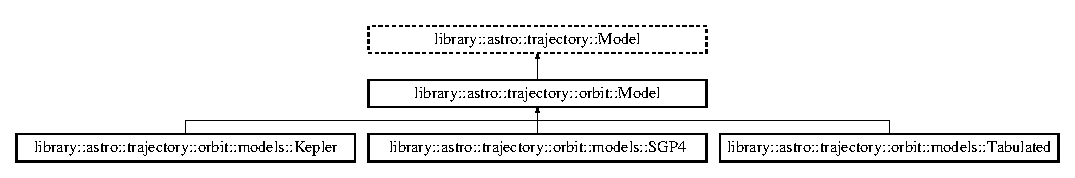
\includegraphics[height=1.944444cm]{classlibrary_1_1astro_1_1trajectory_1_1orbit_1_1_model}
\end{center}
\end{figure}
\subsection*{Public Member Functions}
\begin{DoxyCompactItemize}
\item 
\hyperlink{classlibrary_1_1astro_1_1trajectory_1_1orbit_1_1_model_abcd99755e4229e41638ce373a0e6763c}{Model} ()
\item 
virtual \hyperlink{classlibrary_1_1astro_1_1trajectory_1_1orbit_1_1_model_a1d580725a826a6d16d2c3d4cf2022a50}{$\sim$\+Model} ()=0
\item 
virtual \hyperlink{classlibrary_1_1astro_1_1trajectory_1_1orbit_1_1_model}{Model} $\ast$ \hyperlink{classlibrary_1_1astro_1_1trajectory_1_1orbit_1_1_model_a45d75e4d212a9bb01aa596eaeeae43ae}{clone} () const =0
\item 
virtual bool \hyperlink{classlibrary_1_1astro_1_1trajectory_1_1orbit_1_1_model_a518785603421d259e427bd0a6ee5e787}{is\+Defined} () const =0
\item 
virtual Instant \hyperlink{classlibrary_1_1astro_1_1trajectory_1_1orbit_1_1_model_acdec7ed6eed001c2ab4ac5442699a316}{get\+Epoch} () const =0
\item 
virtual Integer \hyperlink{classlibrary_1_1astro_1_1trajectory_1_1orbit_1_1_model_a940f5e266feb90ee8264d4c7a8a883f3}{get\+Revolution\+Number\+At\+Epoch} () const =0
\item 
virtual \hyperlink{classlibrary_1_1astro_1_1trajectory_1_1_state}{State} \hyperlink{classlibrary_1_1astro_1_1trajectory_1_1orbit_1_1_model_a34198a504836b9779425da99d964d19c}{calculate\+State\+At} (const Instant \&an\+Instant) const =0
\item 
virtual Integer \hyperlink{classlibrary_1_1astro_1_1trajectory_1_1orbit_1_1_model_a6329db5556ed72aa8ad18515aeaefeab}{calculate\+Revolution\+Number\+At} (const Instant \&an\+Instant) const =0
\item 
virtual void \hyperlink{classlibrary_1_1astro_1_1trajectory_1_1orbit_1_1_model_abd4fb7604274cc8b3589a445db64e98c}{print} (std\+::ostream \&an\+Output\+Stream, bool display\+Decorator=true) const =0
\end{DoxyCompactItemize}


\subsection{Constructor \& Destructor Documentation}
\mbox{\Hypertarget{classlibrary_1_1astro_1_1trajectory_1_1orbit_1_1_model_abcd99755e4229e41638ce373a0e6763c}\label{classlibrary_1_1astro_1_1trajectory_1_1orbit_1_1_model_abcd99755e4229e41638ce373a0e6763c}} 
\index{library\+::astro\+::trajectory\+::orbit\+::\+Model@{library\+::astro\+::trajectory\+::orbit\+::\+Model}!Model@{Model}}
\index{Model@{Model}!library\+::astro\+::trajectory\+::orbit\+::\+Model@{library\+::astro\+::trajectory\+::orbit\+::\+Model}}
\subsubsection{\texorpdfstring{Model()}{Model()}}
{\footnotesize\ttfamily library\+::astro\+::trajectory\+::orbit\+::\+Model\+::\+Model (\begin{DoxyParamCaption}{ }\end{DoxyParamCaption})}

\mbox{\Hypertarget{classlibrary_1_1astro_1_1trajectory_1_1orbit_1_1_model_a1d580725a826a6d16d2c3d4cf2022a50}\label{classlibrary_1_1astro_1_1trajectory_1_1orbit_1_1_model_a1d580725a826a6d16d2c3d4cf2022a50}} 
\index{library\+::astro\+::trajectory\+::orbit\+::\+Model@{library\+::astro\+::trajectory\+::orbit\+::\+Model}!````~Model@{$\sim$\+Model}}
\index{````~Model@{$\sim$\+Model}!library\+::astro\+::trajectory\+::orbit\+::\+Model@{library\+::astro\+::trajectory\+::orbit\+::\+Model}}
\subsubsection{\texorpdfstring{$\sim$\+Model()}{~Model()}}
{\footnotesize\ttfamily library\+::astro\+::trajectory\+::orbit\+::\+Model\+::$\sim$\+Model (\begin{DoxyParamCaption}{ }\end{DoxyParamCaption})\hspace{0.3cm}{\ttfamily [pure virtual]}}



Implements \hyperlink{classlibrary_1_1astro_1_1trajectory_1_1_model_abd305caa6adde24bf7ee2eb93e0639d1}{library\+::astro\+::trajectory\+::\+Model}.



\subsection{Member Function Documentation}
\mbox{\Hypertarget{classlibrary_1_1astro_1_1trajectory_1_1orbit_1_1_model_a6329db5556ed72aa8ad18515aeaefeab}\label{classlibrary_1_1astro_1_1trajectory_1_1orbit_1_1_model_a6329db5556ed72aa8ad18515aeaefeab}} 
\index{library\+::astro\+::trajectory\+::orbit\+::\+Model@{library\+::astro\+::trajectory\+::orbit\+::\+Model}!calculate\+Revolution\+Number\+At@{calculate\+Revolution\+Number\+At}}
\index{calculate\+Revolution\+Number\+At@{calculate\+Revolution\+Number\+At}!library\+::astro\+::trajectory\+::orbit\+::\+Model@{library\+::astro\+::trajectory\+::orbit\+::\+Model}}
\subsubsection{\texorpdfstring{calculate\+Revolution\+Number\+At()}{calculateRevolutionNumberAt()}}
{\footnotesize\ttfamily virtual Integer library\+::astro\+::trajectory\+::orbit\+::\+Model\+::calculate\+Revolution\+Number\+At (\begin{DoxyParamCaption}\item[{const Instant \&}]{an\+Instant }\end{DoxyParamCaption}) const\hspace{0.3cm}{\ttfamily [pure virtual]}}



Implemented in \hyperlink{classlibrary_1_1astro_1_1trajectory_1_1orbit_1_1models_1_1_kepler_a9ba435e737c10933f39d4817306810eb}{library\+::astro\+::trajectory\+::orbit\+::models\+::\+Kepler}, \hyperlink{classlibrary_1_1astro_1_1trajectory_1_1orbit_1_1models_1_1_s_g_p4_af1591139c936dd0c696972e5cb461009}{library\+::astro\+::trajectory\+::orbit\+::models\+::\+S\+G\+P4}, and \hyperlink{classlibrary_1_1astro_1_1trajectory_1_1orbit_1_1models_1_1_tabulated_aef0c3d3790f5399c9ae9f78a543a9d5b}{library\+::astro\+::trajectory\+::orbit\+::models\+::\+Tabulated}.

\mbox{\Hypertarget{classlibrary_1_1astro_1_1trajectory_1_1orbit_1_1_model_a34198a504836b9779425da99d964d19c}\label{classlibrary_1_1astro_1_1trajectory_1_1orbit_1_1_model_a34198a504836b9779425da99d964d19c}} 
\index{library\+::astro\+::trajectory\+::orbit\+::\+Model@{library\+::astro\+::trajectory\+::orbit\+::\+Model}!calculate\+State\+At@{calculate\+State\+At}}
\index{calculate\+State\+At@{calculate\+State\+At}!library\+::astro\+::trajectory\+::orbit\+::\+Model@{library\+::astro\+::trajectory\+::orbit\+::\+Model}}
\subsubsection{\texorpdfstring{calculate\+State\+At()}{calculateStateAt()}}
{\footnotesize\ttfamily virtual \hyperlink{classlibrary_1_1astro_1_1trajectory_1_1_state}{State} library\+::astro\+::trajectory\+::orbit\+::\+Model\+::calculate\+State\+At (\begin{DoxyParamCaption}\item[{const Instant \&}]{an\+Instant }\end{DoxyParamCaption}) const\hspace{0.3cm}{\ttfamily [pure virtual]}}



Implements \hyperlink{classlibrary_1_1astro_1_1trajectory_1_1_model_acee9ee770c2ee1d1205b618e8f722ba4}{library\+::astro\+::trajectory\+::\+Model}.



Implemented in \hyperlink{classlibrary_1_1astro_1_1trajectory_1_1orbit_1_1models_1_1_kepler_a6354b3545decf1179289383679ebe2cd}{library\+::astro\+::trajectory\+::orbit\+::models\+::\+Kepler}, \hyperlink{classlibrary_1_1astro_1_1trajectory_1_1orbit_1_1models_1_1_s_g_p4_a5d94d349c464f7313017c795a9346084}{library\+::astro\+::trajectory\+::orbit\+::models\+::\+S\+G\+P4}, and \hyperlink{classlibrary_1_1astro_1_1trajectory_1_1orbit_1_1models_1_1_tabulated_a43db203d7257d25a5a3a6f0e03e62b7d}{library\+::astro\+::trajectory\+::orbit\+::models\+::\+Tabulated}.

\mbox{\Hypertarget{classlibrary_1_1astro_1_1trajectory_1_1orbit_1_1_model_a45d75e4d212a9bb01aa596eaeeae43ae}\label{classlibrary_1_1astro_1_1trajectory_1_1orbit_1_1_model_a45d75e4d212a9bb01aa596eaeeae43ae}} 
\index{library\+::astro\+::trajectory\+::orbit\+::\+Model@{library\+::astro\+::trajectory\+::orbit\+::\+Model}!clone@{clone}}
\index{clone@{clone}!library\+::astro\+::trajectory\+::orbit\+::\+Model@{library\+::astro\+::trajectory\+::orbit\+::\+Model}}
\subsubsection{\texorpdfstring{clone()}{clone()}}
{\footnotesize\ttfamily virtual \hyperlink{classlibrary_1_1astro_1_1trajectory_1_1orbit_1_1_model}{Model}$\ast$ library\+::astro\+::trajectory\+::orbit\+::\+Model\+::clone (\begin{DoxyParamCaption}{ }\end{DoxyParamCaption}) const\hspace{0.3cm}{\ttfamily [pure virtual]}}



Implements \hyperlink{classlibrary_1_1astro_1_1trajectory_1_1_model_ad6181e14aea57534897e7446a2a27578}{library\+::astro\+::trajectory\+::\+Model}.



Implemented in \hyperlink{classlibrary_1_1astro_1_1trajectory_1_1orbit_1_1models_1_1_kepler_ac78a023cde4a61c62309051c9147d66e}{library\+::astro\+::trajectory\+::orbit\+::models\+::\+Kepler}, \hyperlink{classlibrary_1_1astro_1_1trajectory_1_1orbit_1_1models_1_1_s_g_p4_afa3add6c6855ac1da5632b17986dca02}{library\+::astro\+::trajectory\+::orbit\+::models\+::\+S\+G\+P4}, and \hyperlink{classlibrary_1_1astro_1_1trajectory_1_1orbit_1_1models_1_1_tabulated_a8ccec23a49086c6c3fbda2cc81e7a4dc}{library\+::astro\+::trajectory\+::orbit\+::models\+::\+Tabulated}.

\mbox{\Hypertarget{classlibrary_1_1astro_1_1trajectory_1_1orbit_1_1_model_acdec7ed6eed001c2ab4ac5442699a316}\label{classlibrary_1_1astro_1_1trajectory_1_1orbit_1_1_model_acdec7ed6eed001c2ab4ac5442699a316}} 
\index{library\+::astro\+::trajectory\+::orbit\+::\+Model@{library\+::astro\+::trajectory\+::orbit\+::\+Model}!get\+Epoch@{get\+Epoch}}
\index{get\+Epoch@{get\+Epoch}!library\+::astro\+::trajectory\+::orbit\+::\+Model@{library\+::astro\+::trajectory\+::orbit\+::\+Model}}
\subsubsection{\texorpdfstring{get\+Epoch()}{getEpoch()}}
{\footnotesize\ttfamily virtual Instant library\+::astro\+::trajectory\+::orbit\+::\+Model\+::get\+Epoch (\begin{DoxyParamCaption}{ }\end{DoxyParamCaption}) const\hspace{0.3cm}{\ttfamily [pure virtual]}}



Implemented in \hyperlink{classlibrary_1_1astro_1_1trajectory_1_1orbit_1_1models_1_1_kepler_a6ecdd4a133cdd936909020b644dd8f1f}{library\+::astro\+::trajectory\+::orbit\+::models\+::\+Kepler}, \hyperlink{classlibrary_1_1astro_1_1trajectory_1_1orbit_1_1models_1_1_s_g_p4_a44439cf23b0d6d7b726b5b9c8784b5c1}{library\+::astro\+::trajectory\+::orbit\+::models\+::\+S\+G\+P4}, and \hyperlink{classlibrary_1_1astro_1_1trajectory_1_1orbit_1_1models_1_1_tabulated_a9e12e7f7b79bf8d2d37494ff7a55ae1d}{library\+::astro\+::trajectory\+::orbit\+::models\+::\+Tabulated}.

\mbox{\Hypertarget{classlibrary_1_1astro_1_1trajectory_1_1orbit_1_1_model_a940f5e266feb90ee8264d4c7a8a883f3}\label{classlibrary_1_1astro_1_1trajectory_1_1orbit_1_1_model_a940f5e266feb90ee8264d4c7a8a883f3}} 
\index{library\+::astro\+::trajectory\+::orbit\+::\+Model@{library\+::astro\+::trajectory\+::orbit\+::\+Model}!get\+Revolution\+Number\+At\+Epoch@{get\+Revolution\+Number\+At\+Epoch}}
\index{get\+Revolution\+Number\+At\+Epoch@{get\+Revolution\+Number\+At\+Epoch}!library\+::astro\+::trajectory\+::orbit\+::\+Model@{library\+::astro\+::trajectory\+::orbit\+::\+Model}}
\subsubsection{\texorpdfstring{get\+Revolution\+Number\+At\+Epoch()}{getRevolutionNumberAtEpoch()}}
{\footnotesize\ttfamily virtual Integer library\+::astro\+::trajectory\+::orbit\+::\+Model\+::get\+Revolution\+Number\+At\+Epoch (\begin{DoxyParamCaption}{ }\end{DoxyParamCaption}) const\hspace{0.3cm}{\ttfamily [pure virtual]}}



Implemented in \hyperlink{classlibrary_1_1astro_1_1trajectory_1_1orbit_1_1models_1_1_kepler_ad8df985c06ca56c1516f3b8804d5052d}{library\+::astro\+::trajectory\+::orbit\+::models\+::\+Kepler}, \hyperlink{classlibrary_1_1astro_1_1trajectory_1_1orbit_1_1models_1_1_s_g_p4_ac4b0a82cff7908a0192b7e2db3107f13}{library\+::astro\+::trajectory\+::orbit\+::models\+::\+S\+G\+P4}, and \hyperlink{classlibrary_1_1astro_1_1trajectory_1_1orbit_1_1models_1_1_tabulated_aece7054c261932c3298e8ef2faa2d588}{library\+::astro\+::trajectory\+::orbit\+::models\+::\+Tabulated}.

\mbox{\Hypertarget{classlibrary_1_1astro_1_1trajectory_1_1orbit_1_1_model_a518785603421d259e427bd0a6ee5e787}\label{classlibrary_1_1astro_1_1trajectory_1_1orbit_1_1_model_a518785603421d259e427bd0a6ee5e787}} 
\index{library\+::astro\+::trajectory\+::orbit\+::\+Model@{library\+::astro\+::trajectory\+::orbit\+::\+Model}!is\+Defined@{is\+Defined}}
\index{is\+Defined@{is\+Defined}!library\+::astro\+::trajectory\+::orbit\+::\+Model@{library\+::astro\+::trajectory\+::orbit\+::\+Model}}
\subsubsection{\texorpdfstring{is\+Defined()}{isDefined()}}
{\footnotesize\ttfamily virtual bool library\+::astro\+::trajectory\+::orbit\+::\+Model\+::is\+Defined (\begin{DoxyParamCaption}{ }\end{DoxyParamCaption}) const\hspace{0.3cm}{\ttfamily [pure virtual]}}



Implements \hyperlink{classlibrary_1_1astro_1_1trajectory_1_1_model_a9b55db62f22c3493313661bacd9f7c1b}{library\+::astro\+::trajectory\+::\+Model}.



Implemented in \hyperlink{classlibrary_1_1astro_1_1trajectory_1_1orbit_1_1models_1_1_kepler_a600d7752a50924ee6e3fc08f18a229e9}{library\+::astro\+::trajectory\+::orbit\+::models\+::\+Kepler}, \hyperlink{classlibrary_1_1astro_1_1trajectory_1_1orbit_1_1models_1_1_s_g_p4_a2d70ef4601e453156a430115e11ce8d7}{library\+::astro\+::trajectory\+::orbit\+::models\+::\+S\+G\+P4}, and \hyperlink{classlibrary_1_1astro_1_1trajectory_1_1orbit_1_1models_1_1_tabulated_af68120eb6651e8461c02a465923e533f}{library\+::astro\+::trajectory\+::orbit\+::models\+::\+Tabulated}.

\mbox{\Hypertarget{classlibrary_1_1astro_1_1trajectory_1_1orbit_1_1_model_abd4fb7604274cc8b3589a445db64e98c}\label{classlibrary_1_1astro_1_1trajectory_1_1orbit_1_1_model_abd4fb7604274cc8b3589a445db64e98c}} 
\index{library\+::astro\+::trajectory\+::orbit\+::\+Model@{library\+::astro\+::trajectory\+::orbit\+::\+Model}!print@{print}}
\index{print@{print}!library\+::astro\+::trajectory\+::orbit\+::\+Model@{library\+::astro\+::trajectory\+::orbit\+::\+Model}}
\subsubsection{\texorpdfstring{print()}{print()}}
{\footnotesize\ttfamily virtual void library\+::astro\+::trajectory\+::orbit\+::\+Model\+::print (\begin{DoxyParamCaption}\item[{std\+::ostream \&}]{an\+Output\+Stream,  }\item[{bool}]{display\+Decorator = {\ttfamily true} }\end{DoxyParamCaption}) const\hspace{0.3cm}{\ttfamily [pure virtual]}}



Implements \hyperlink{classlibrary_1_1astro_1_1trajectory_1_1_model_af3dd0c38fdbac0b64f689fd8c88c3320}{library\+::astro\+::trajectory\+::\+Model}.



Implemented in \hyperlink{classlibrary_1_1astro_1_1trajectory_1_1orbit_1_1models_1_1_kepler_a5cecedfe1b2002881b4ef6eeae64af93}{library\+::astro\+::trajectory\+::orbit\+::models\+::\+Kepler}, \hyperlink{classlibrary_1_1astro_1_1trajectory_1_1orbit_1_1models_1_1_s_g_p4_aca7d5615c14d59338506fb13630cd535}{library\+::astro\+::trajectory\+::orbit\+::models\+::\+S\+G\+P4}, and \hyperlink{classlibrary_1_1astro_1_1trajectory_1_1orbit_1_1models_1_1_tabulated_a545a7209580a0c3863f37e2bdd925cb6}{library\+::astro\+::trajectory\+::orbit\+::models\+::\+Tabulated}.



The documentation for this class was generated from the following files\+:\begin{DoxyCompactItemize}
\item 
include/\+Library/\+Astrodynamics/\+Trajectory/\+Orbit/\hyperlink{_orbit_2_model_8hpp}{Model.\+hpp}\item 
src/\+Library/\+Astrodynamics/\+Trajectory/\+Orbit/\hyperlink{_orbit_2_model_8cpp}{Model.\+cpp}\end{DoxyCompactItemize}

\hypertarget{classlibrary_1_1astro_1_1trajectory_1_1_model}{}\section{library\+:\+:astro\+:\+:trajectory\+:\+:Model Class Reference}
\label{classlibrary_1_1astro_1_1trajectory_1_1_model}\index{library\+::astro\+::trajectory\+::\+Model@{library\+::astro\+::trajectory\+::\+Model}}


\hyperlink{classlibrary_1_1astro_1_1_trajectory}{Trajectory} model (abstract)  




{\ttfamily \#include $<$Model.\+hpp$>$}

Inheritance diagram for library\+:\+:astro\+:\+:trajectory\+:\+:Model\+:\begin{figure}[H]
\begin{center}
\leavevmode
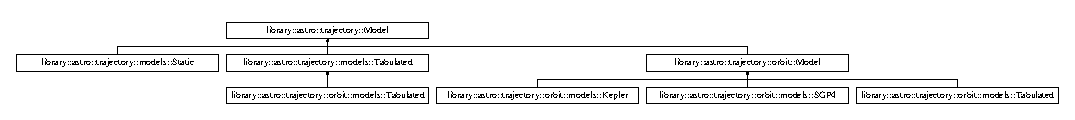
\includegraphics[height=1.166667cm]{classlibrary_1_1astro_1_1trajectory_1_1_model}
\end{center}
\end{figure}
\subsection*{Public Member Functions}
\begin{DoxyCompactItemize}
\item 
\hyperlink{classlibrary_1_1astro_1_1trajectory_1_1_model_a083bde3f2c8d3d1406220ad3e2dd9cd9}{Model} ()
\item 
virtual \hyperlink{classlibrary_1_1astro_1_1trajectory_1_1_model_abd305caa6adde24bf7ee2eb93e0639d1}{$\sim$\+Model} ()=0
\item 
virtual \hyperlink{classlibrary_1_1astro_1_1trajectory_1_1_model}{Model} $\ast$ \hyperlink{classlibrary_1_1astro_1_1trajectory_1_1_model_ad6181e14aea57534897e7446a2a27578}{clone} () const =0
\item 
virtual bool \hyperlink{classlibrary_1_1astro_1_1trajectory_1_1_model_a83c52eb23e8feea58d600c87700ed923}{operator==} (const \hyperlink{classlibrary_1_1astro_1_1trajectory_1_1_model}{Model} \&a\+Model) const =0
\item 
virtual bool \hyperlink{classlibrary_1_1astro_1_1trajectory_1_1_model_a476c234f5fca1eb75f64f5a96fd83c61}{operator!=} (const \hyperlink{classlibrary_1_1astro_1_1trajectory_1_1_model}{Model} \&a\+Model) const =0
\item 
virtual bool \hyperlink{classlibrary_1_1astro_1_1trajectory_1_1_model_a9b55db62f22c3493313661bacd9f7c1b}{is\+Defined} () const =0
\item 
{\footnotesize template$<$class Type $>$ }\\bool \hyperlink{classlibrary_1_1astro_1_1trajectory_1_1_model_ad8444d9fcab4f6a95d42fca5d397fe0f}{is} () const
\begin{DoxyCompactList}\small\item\em Returns true if model can be converted to type. \end{DoxyCompactList}\item 
{\footnotesize template$<$class Type $>$ }\\const Type \& \hyperlink{classlibrary_1_1astro_1_1trajectory_1_1_model_a6f03598834d74ef1e03ce3469e892e6c}{as} () const
\begin{DoxyCompactList}\small\item\em \hyperlink{classlibrary_1_1astro_1_1_access}{Access} model as its underlying type. \end{DoxyCompactList}\item 
virtual \hyperlink{classlibrary_1_1astro_1_1trajectory_1_1_state}{State} \hyperlink{classlibrary_1_1astro_1_1trajectory_1_1_model_acee9ee770c2ee1d1205b618e8f722ba4}{calculate\+State\+At} (const Instant \&an\+Instant) const =0
\item 
virtual void \hyperlink{classlibrary_1_1astro_1_1trajectory_1_1_model_af3dd0c38fdbac0b64f689fd8c88c3320}{print} (std\+::ostream \&an\+Output\+Stream, bool display\+Decorator=true) const =0
\end{DoxyCompactItemize}
\subsection*{Friends}
\begin{DoxyCompactItemize}
\item 
std\+::ostream \& \hyperlink{classlibrary_1_1astro_1_1trajectory_1_1_model_a68240493d08f91f6613186eb52823e85}{operator$<$$<$} (std\+::ostream \&an\+Output\+Stream, const \hyperlink{classlibrary_1_1astro_1_1trajectory_1_1_model}{Model} \&a\+Model)
\end{DoxyCompactItemize}


\subsection{Detailed Description}
\hyperlink{classlibrary_1_1astro_1_1_trajectory}{Trajectory} model (abstract) 

\subsection{Constructor \& Destructor Documentation}
\mbox{\Hypertarget{classlibrary_1_1astro_1_1trajectory_1_1_model_a083bde3f2c8d3d1406220ad3e2dd9cd9}\label{classlibrary_1_1astro_1_1trajectory_1_1_model_a083bde3f2c8d3d1406220ad3e2dd9cd9}} 
\index{library\+::astro\+::trajectory\+::\+Model@{library\+::astro\+::trajectory\+::\+Model}!Model@{Model}}
\index{Model@{Model}!library\+::astro\+::trajectory\+::\+Model@{library\+::astro\+::trajectory\+::\+Model}}
\subsubsection{\texorpdfstring{Model()}{Model()}}
{\footnotesize\ttfamily library\+::astro\+::trajectory\+::\+Model\+::\+Model (\begin{DoxyParamCaption}{ }\end{DoxyParamCaption})}

\mbox{\Hypertarget{classlibrary_1_1astro_1_1trajectory_1_1_model_abd305caa6adde24bf7ee2eb93e0639d1}\label{classlibrary_1_1astro_1_1trajectory_1_1_model_abd305caa6adde24bf7ee2eb93e0639d1}} 
\index{library\+::astro\+::trajectory\+::\+Model@{library\+::astro\+::trajectory\+::\+Model}!````~Model@{$\sim$\+Model}}
\index{````~Model@{$\sim$\+Model}!library\+::astro\+::trajectory\+::\+Model@{library\+::astro\+::trajectory\+::\+Model}}
\subsubsection{\texorpdfstring{$\sim$\+Model()}{~Model()}}
{\footnotesize\ttfamily library\+::astro\+::trajectory\+::\+Model\+::$\sim$\+Model (\begin{DoxyParamCaption}{ }\end{DoxyParamCaption})\hspace{0.3cm}{\ttfamily [pure virtual]}}



Implemented in \hyperlink{classlibrary_1_1astro_1_1trajectory_1_1orbit_1_1_model_a1d580725a826a6d16d2c3d4cf2022a50}{library\+::astro\+::trajectory\+::orbit\+::\+Model}.



\subsection{Member Function Documentation}
\mbox{\Hypertarget{classlibrary_1_1astro_1_1trajectory_1_1_model_a6f03598834d74ef1e03ce3469e892e6c}\label{classlibrary_1_1astro_1_1trajectory_1_1_model_a6f03598834d74ef1e03ce3469e892e6c}} 
\index{library\+::astro\+::trajectory\+::\+Model@{library\+::astro\+::trajectory\+::\+Model}!as@{as}}
\index{as@{as}!library\+::astro\+::trajectory\+::\+Model@{library\+::astro\+::trajectory\+::\+Model}}
\subsubsection{\texorpdfstring{as()}{as()}}
{\footnotesize\ttfamily template$<$class Type $>$ \\
const Type\& library\+::astro\+::trajectory\+::\+Model\+::as (\begin{DoxyParamCaption}{ }\end{DoxyParamCaption}) const\hspace{0.3cm}{\ttfamily [inline]}}



\hyperlink{classlibrary_1_1astro_1_1_access}{Access} model as its underlying type. 

\begin{DoxyReturn}{Returns}
Reference to underlying type 
\end{DoxyReturn}
\mbox{\Hypertarget{classlibrary_1_1astro_1_1trajectory_1_1_model_acee9ee770c2ee1d1205b618e8f722ba4}\label{classlibrary_1_1astro_1_1trajectory_1_1_model_acee9ee770c2ee1d1205b618e8f722ba4}} 
\index{library\+::astro\+::trajectory\+::\+Model@{library\+::astro\+::trajectory\+::\+Model}!calculate\+State\+At@{calculate\+State\+At}}
\index{calculate\+State\+At@{calculate\+State\+At}!library\+::astro\+::trajectory\+::\+Model@{library\+::astro\+::trajectory\+::\+Model}}
\subsubsection{\texorpdfstring{calculate\+State\+At()}{calculateStateAt()}}
{\footnotesize\ttfamily virtual \hyperlink{classlibrary_1_1astro_1_1trajectory_1_1_state}{State} library\+::astro\+::trajectory\+::\+Model\+::calculate\+State\+At (\begin{DoxyParamCaption}\item[{const Instant \&}]{an\+Instant }\end{DoxyParamCaption}) const\hspace{0.3cm}{\ttfamily [pure virtual]}}



Implemented in \hyperlink{classlibrary_1_1astro_1_1trajectory_1_1orbit_1_1models_1_1_kepler_a6354b3545decf1179289383679ebe2cd}{library\+::astro\+::trajectory\+::orbit\+::models\+::\+Kepler}, \hyperlink{classlibrary_1_1astro_1_1trajectory_1_1orbit_1_1models_1_1_s_g_p4_a5d94d349c464f7313017c795a9346084}{library\+::astro\+::trajectory\+::orbit\+::models\+::\+S\+G\+P4}, \hyperlink{classlibrary_1_1astro_1_1trajectory_1_1models_1_1_tabulated_a6d23f5721930d9e885eb3b763ab3390a}{library\+::astro\+::trajectory\+::models\+::\+Tabulated}, \hyperlink{classlibrary_1_1astro_1_1trajectory_1_1orbit_1_1models_1_1_tabulated_a43db203d7257d25a5a3a6f0e03e62b7d}{library\+::astro\+::trajectory\+::orbit\+::models\+::\+Tabulated}, \hyperlink{classlibrary_1_1astro_1_1trajectory_1_1models_1_1_static_ae4bc6aceab498868e4ebe2a65c6aa413}{library\+::astro\+::trajectory\+::models\+::\+Static}, and \hyperlink{classlibrary_1_1astro_1_1trajectory_1_1orbit_1_1_model_a34198a504836b9779425da99d964d19c}{library\+::astro\+::trajectory\+::orbit\+::\+Model}.

\mbox{\Hypertarget{classlibrary_1_1astro_1_1trajectory_1_1_model_ad6181e14aea57534897e7446a2a27578}\label{classlibrary_1_1astro_1_1trajectory_1_1_model_ad6181e14aea57534897e7446a2a27578}} 
\index{library\+::astro\+::trajectory\+::\+Model@{library\+::astro\+::trajectory\+::\+Model}!clone@{clone}}
\index{clone@{clone}!library\+::astro\+::trajectory\+::\+Model@{library\+::astro\+::trajectory\+::\+Model}}
\subsubsection{\texorpdfstring{clone()}{clone()}}
{\footnotesize\ttfamily virtual \hyperlink{classlibrary_1_1astro_1_1trajectory_1_1_model}{Model}$\ast$ library\+::astro\+::trajectory\+::\+Model\+::clone (\begin{DoxyParamCaption}{ }\end{DoxyParamCaption}) const\hspace{0.3cm}{\ttfamily [pure virtual]}}



Implemented in \hyperlink{classlibrary_1_1astro_1_1trajectory_1_1orbit_1_1models_1_1_kepler_ac78a023cde4a61c62309051c9147d66e}{library\+::astro\+::trajectory\+::orbit\+::models\+::\+Kepler}, \hyperlink{classlibrary_1_1astro_1_1trajectory_1_1orbit_1_1models_1_1_s_g_p4_afa3add6c6855ac1da5632b17986dca02}{library\+::astro\+::trajectory\+::orbit\+::models\+::\+S\+G\+P4}, \hyperlink{classlibrary_1_1astro_1_1trajectory_1_1models_1_1_tabulated_a192cfb0ceb4a11d02578adc9702cabc1}{library\+::astro\+::trajectory\+::models\+::\+Tabulated}, \hyperlink{classlibrary_1_1astro_1_1trajectory_1_1orbit_1_1models_1_1_tabulated_a8ccec23a49086c6c3fbda2cc81e7a4dc}{library\+::astro\+::trajectory\+::orbit\+::models\+::\+Tabulated}, \hyperlink{classlibrary_1_1astro_1_1trajectory_1_1models_1_1_static_a3586bbfdd6fc3958b18a2ffcb3b23fd4}{library\+::astro\+::trajectory\+::models\+::\+Static}, and \hyperlink{classlibrary_1_1astro_1_1trajectory_1_1orbit_1_1_model_a45d75e4d212a9bb01aa596eaeeae43ae}{library\+::astro\+::trajectory\+::orbit\+::\+Model}.

\mbox{\Hypertarget{classlibrary_1_1astro_1_1trajectory_1_1_model_ad8444d9fcab4f6a95d42fca5d397fe0f}\label{classlibrary_1_1astro_1_1trajectory_1_1_model_ad8444d9fcab4f6a95d42fca5d397fe0f}} 
\index{library\+::astro\+::trajectory\+::\+Model@{library\+::astro\+::trajectory\+::\+Model}!is@{is}}
\index{is@{is}!library\+::astro\+::trajectory\+::\+Model@{library\+::astro\+::trajectory\+::\+Model}}
\subsubsection{\texorpdfstring{is()}{is()}}
{\footnotesize\ttfamily template$<$class Type $>$ \\
bool library\+::astro\+::trajectory\+::\+Model\+::is (\begin{DoxyParamCaption}{ }\end{DoxyParamCaption}) const\hspace{0.3cm}{\ttfamily [inline]}}



Returns true if model can be converted to type. 

\begin{DoxyReturn}{Returns}
True if model can be converted to type 
\end{DoxyReturn}
\mbox{\Hypertarget{classlibrary_1_1astro_1_1trajectory_1_1_model_a9b55db62f22c3493313661bacd9f7c1b}\label{classlibrary_1_1astro_1_1trajectory_1_1_model_a9b55db62f22c3493313661bacd9f7c1b}} 
\index{library\+::astro\+::trajectory\+::\+Model@{library\+::astro\+::trajectory\+::\+Model}!is\+Defined@{is\+Defined}}
\index{is\+Defined@{is\+Defined}!library\+::astro\+::trajectory\+::\+Model@{library\+::astro\+::trajectory\+::\+Model}}
\subsubsection{\texorpdfstring{is\+Defined()}{isDefined()}}
{\footnotesize\ttfamily virtual bool library\+::astro\+::trajectory\+::\+Model\+::is\+Defined (\begin{DoxyParamCaption}{ }\end{DoxyParamCaption}) const\hspace{0.3cm}{\ttfamily [pure virtual]}}



Implemented in \hyperlink{classlibrary_1_1astro_1_1trajectory_1_1orbit_1_1models_1_1_kepler_a600d7752a50924ee6e3fc08f18a229e9}{library\+::astro\+::trajectory\+::orbit\+::models\+::\+Kepler}, \hyperlink{classlibrary_1_1astro_1_1trajectory_1_1orbit_1_1models_1_1_s_g_p4_a2d70ef4601e453156a430115e11ce8d7}{library\+::astro\+::trajectory\+::orbit\+::models\+::\+S\+G\+P4}, \hyperlink{classlibrary_1_1astro_1_1trajectory_1_1models_1_1_tabulated_ae967e30f6de74405671f992a5920883f}{library\+::astro\+::trajectory\+::models\+::\+Tabulated}, \hyperlink{classlibrary_1_1astro_1_1trajectory_1_1orbit_1_1models_1_1_tabulated_af68120eb6651e8461c02a465923e533f}{library\+::astro\+::trajectory\+::orbit\+::models\+::\+Tabulated}, \hyperlink{classlibrary_1_1astro_1_1trajectory_1_1models_1_1_static_a41449e98bb076e0601df67b1cfbff6b8}{library\+::astro\+::trajectory\+::models\+::\+Static}, and \hyperlink{classlibrary_1_1astro_1_1trajectory_1_1orbit_1_1_model_a518785603421d259e427bd0a6ee5e787}{library\+::astro\+::trajectory\+::orbit\+::\+Model}.

\mbox{\Hypertarget{classlibrary_1_1astro_1_1trajectory_1_1_model_a476c234f5fca1eb75f64f5a96fd83c61}\label{classlibrary_1_1astro_1_1trajectory_1_1_model_a476c234f5fca1eb75f64f5a96fd83c61}} 
\index{library\+::astro\+::trajectory\+::\+Model@{library\+::astro\+::trajectory\+::\+Model}!operator"!=@{operator"!=}}
\index{operator"!=@{operator"!=}!library\+::astro\+::trajectory\+::\+Model@{library\+::astro\+::trajectory\+::\+Model}}
\subsubsection{\texorpdfstring{operator"!=()}{operator!=()}}
{\footnotesize\ttfamily virtual bool library\+::astro\+::trajectory\+::\+Model\+::operator!= (\begin{DoxyParamCaption}\item[{const \hyperlink{classlibrary_1_1astro_1_1trajectory_1_1_model}{Model} \&}]{a\+Model }\end{DoxyParamCaption}) const\hspace{0.3cm}{\ttfamily [pure virtual]}}



Implemented in \hyperlink{classlibrary_1_1astro_1_1trajectory_1_1orbit_1_1models_1_1_kepler_a2671d995d476b11a14cc08aad2dc0b30}{library\+::astro\+::trajectory\+::orbit\+::models\+::\+Kepler}, \hyperlink{classlibrary_1_1astro_1_1trajectory_1_1orbit_1_1models_1_1_s_g_p4_addbc5d1289986a6f89da00a21d4ab8e6}{library\+::astro\+::trajectory\+::orbit\+::models\+::\+S\+G\+P4}, \hyperlink{classlibrary_1_1astro_1_1trajectory_1_1models_1_1_tabulated_ae6b286af87f28d080b523fb879b74109}{library\+::astro\+::trajectory\+::models\+::\+Tabulated}, \hyperlink{classlibrary_1_1astro_1_1trajectory_1_1orbit_1_1models_1_1_tabulated_a4373b98c6026c999da98e1740c784e17}{library\+::astro\+::trajectory\+::orbit\+::models\+::\+Tabulated}, and \hyperlink{classlibrary_1_1astro_1_1trajectory_1_1models_1_1_static_aadcfd4ac66cc3fc4cc2b868b9bbc182a}{library\+::astro\+::trajectory\+::models\+::\+Static}.

\mbox{\Hypertarget{classlibrary_1_1astro_1_1trajectory_1_1_model_a83c52eb23e8feea58d600c87700ed923}\label{classlibrary_1_1astro_1_1trajectory_1_1_model_a83c52eb23e8feea58d600c87700ed923}} 
\index{library\+::astro\+::trajectory\+::\+Model@{library\+::astro\+::trajectory\+::\+Model}!operator==@{operator==}}
\index{operator==@{operator==}!library\+::astro\+::trajectory\+::\+Model@{library\+::astro\+::trajectory\+::\+Model}}
\subsubsection{\texorpdfstring{operator==()}{operator==()}}
{\footnotesize\ttfamily virtual bool library\+::astro\+::trajectory\+::\+Model\+::operator== (\begin{DoxyParamCaption}\item[{const \hyperlink{classlibrary_1_1astro_1_1trajectory_1_1_model}{Model} \&}]{a\+Model }\end{DoxyParamCaption}) const\hspace{0.3cm}{\ttfamily [pure virtual]}}



Implemented in \hyperlink{classlibrary_1_1astro_1_1trajectory_1_1orbit_1_1models_1_1_kepler_af3adc1e4bee0a3064963209b58178e98}{library\+::astro\+::trajectory\+::orbit\+::models\+::\+Kepler}, \hyperlink{classlibrary_1_1astro_1_1trajectory_1_1orbit_1_1models_1_1_s_g_p4_a6210273bf78e8b98b310999a09d89cc4}{library\+::astro\+::trajectory\+::orbit\+::models\+::\+S\+G\+P4}, \hyperlink{classlibrary_1_1astro_1_1trajectory_1_1models_1_1_tabulated_af733fafd705bd6a1f204acdbaf2e9646}{library\+::astro\+::trajectory\+::models\+::\+Tabulated}, \hyperlink{classlibrary_1_1astro_1_1trajectory_1_1orbit_1_1models_1_1_tabulated_a7194a96e062cb6a8c109c82e169a9d7d}{library\+::astro\+::trajectory\+::orbit\+::models\+::\+Tabulated}, and \hyperlink{classlibrary_1_1astro_1_1trajectory_1_1models_1_1_static_ade92be03b036c9625bd5a4111cb69731}{library\+::astro\+::trajectory\+::models\+::\+Static}.

\mbox{\Hypertarget{classlibrary_1_1astro_1_1trajectory_1_1_model_af3dd0c38fdbac0b64f689fd8c88c3320}\label{classlibrary_1_1astro_1_1trajectory_1_1_model_af3dd0c38fdbac0b64f689fd8c88c3320}} 
\index{library\+::astro\+::trajectory\+::\+Model@{library\+::astro\+::trajectory\+::\+Model}!print@{print}}
\index{print@{print}!library\+::astro\+::trajectory\+::\+Model@{library\+::astro\+::trajectory\+::\+Model}}
\subsubsection{\texorpdfstring{print()}{print()}}
{\footnotesize\ttfamily virtual void library\+::astro\+::trajectory\+::\+Model\+::print (\begin{DoxyParamCaption}\item[{std\+::ostream \&}]{an\+Output\+Stream,  }\item[{bool}]{display\+Decorator = {\ttfamily true} }\end{DoxyParamCaption}) const\hspace{0.3cm}{\ttfamily [pure virtual]}}



Implemented in \hyperlink{classlibrary_1_1astro_1_1trajectory_1_1orbit_1_1models_1_1_kepler_a5cecedfe1b2002881b4ef6eeae64af93}{library\+::astro\+::trajectory\+::orbit\+::models\+::\+Kepler}, \hyperlink{classlibrary_1_1astro_1_1trajectory_1_1orbit_1_1models_1_1_s_g_p4_aca7d5615c14d59338506fb13630cd535}{library\+::astro\+::trajectory\+::orbit\+::models\+::\+S\+G\+P4}, \hyperlink{classlibrary_1_1astro_1_1trajectory_1_1models_1_1_tabulated_a3eae12849178fe43d30a620edceddd8e}{library\+::astro\+::trajectory\+::models\+::\+Tabulated}, \hyperlink{classlibrary_1_1astro_1_1trajectory_1_1orbit_1_1models_1_1_tabulated_a545a7209580a0c3863f37e2bdd925cb6}{library\+::astro\+::trajectory\+::orbit\+::models\+::\+Tabulated}, \hyperlink{classlibrary_1_1astro_1_1trajectory_1_1models_1_1_static_af8f9c6fa6ae2d4471868cc970e1ef571}{library\+::astro\+::trajectory\+::models\+::\+Static}, and \hyperlink{classlibrary_1_1astro_1_1trajectory_1_1orbit_1_1_model_abd4fb7604274cc8b3589a445db64e98c}{library\+::astro\+::trajectory\+::orbit\+::\+Model}.



\subsection{Friends And Related Function Documentation}
\mbox{\Hypertarget{classlibrary_1_1astro_1_1trajectory_1_1_model_a68240493d08f91f6613186eb52823e85}\label{classlibrary_1_1astro_1_1trajectory_1_1_model_a68240493d08f91f6613186eb52823e85}} 
\index{library\+::astro\+::trajectory\+::\+Model@{library\+::astro\+::trajectory\+::\+Model}!operator$<$$<$@{operator$<$$<$}}
\index{operator$<$$<$@{operator$<$$<$}!library\+::astro\+::trajectory\+::\+Model@{library\+::astro\+::trajectory\+::\+Model}}
\subsubsection{\texorpdfstring{operator$<$$<$}{operator<<}}
{\footnotesize\ttfamily std\+::ostream\& operator$<$$<$ (\begin{DoxyParamCaption}\item[{std\+::ostream \&}]{an\+Output\+Stream,  }\item[{const \hyperlink{classlibrary_1_1astro_1_1trajectory_1_1_model}{Model} \&}]{a\+Model }\end{DoxyParamCaption})\hspace{0.3cm}{\ttfamily [friend]}}



The documentation for this class was generated from the following files\+:\begin{DoxyCompactItemize}
\item 
include/\+Library/\+Astrodynamics/\+Trajectory/\hyperlink{_model_8hpp}{Model.\+hpp}\item 
src/\+Library/\+Astrodynamics/\+Trajectory/\hyperlink{_model_8cpp}{Model.\+cpp}\end{DoxyCompactItemize}

\hypertarget{classlibrary_1_1astro_1_1trajectory_1_1_orbit}{}\section{library\+:\+:astro\+:\+:trajectory\+:\+:Orbit Class Reference}
\label{classlibrary_1_1astro_1_1trajectory_1_1_orbit}\index{library\+::astro\+::trajectory\+::\+Orbit@{library\+::astro\+::trajectory\+::\+Orbit}}


Gravitationally curved trajectory of an object.  




{\ttfamily \#include $<$Orbit.\+hpp$>$}

Inheritance diagram for library\+:\+:astro\+:\+:trajectory\+:\+:Orbit\+:\begin{figure}[H]
\begin{center}
\leavevmode
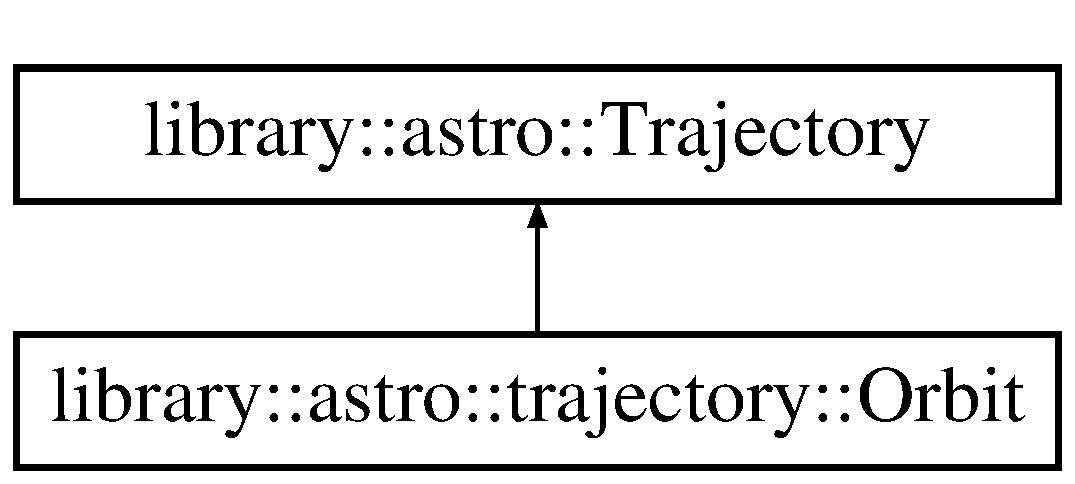
\includegraphics[height=2.000000cm]{classlibrary_1_1astro_1_1trajectory_1_1_orbit}
\end{center}
\end{figure}
\subsection*{Public Types}
\begin{DoxyCompactItemize}
\item 
enum \hyperlink{classlibrary_1_1astro_1_1trajectory_1_1_orbit_a816e83a0c220d4242ce2bebd32191cd8}{Frame\+Type} \{ \newline
\hyperlink{classlibrary_1_1astro_1_1trajectory_1_1_orbit_a816e83a0c220d4242ce2bebd32191cd8aec0fc0100c4fc1ce4eea230c3dc10360}{Frame\+Type\+::\+Undefined}, 
\hyperlink{classlibrary_1_1astro_1_1trajectory_1_1_orbit_a816e83a0c220d4242ce2bebd32191cd8acd3459b28418fa8fa75ffaba4f3e7c74}{Frame\+Type\+::\+N\+ED}, 
\hyperlink{classlibrary_1_1astro_1_1trajectory_1_1_orbit_a816e83a0c220d4242ce2bebd32191cd8acdfe4a5ed313c123b78c17d455cfa94f}{Frame\+Type\+::\+L\+V\+LH}, 
\hyperlink{classlibrary_1_1astro_1_1trajectory_1_1_orbit_a816e83a0c220d4242ce2bebd32191cd8ae01a717c5a8a11cf57f7fdcb96aedc9c}{Frame\+Type\+::\+V\+V\+LH}, 
\newline
\hyperlink{classlibrary_1_1astro_1_1trajectory_1_1_orbit_a816e83a0c220d4242ce2bebd32191cd8a9f24a174bf2de776f4f87caef847746f}{Frame\+Type\+::\+L\+V\+L\+H\+GD}, 
\hyperlink{classlibrary_1_1astro_1_1trajectory_1_1_orbit_a816e83a0c220d4242ce2bebd32191cd8a4f190ed692b3a94eb49da59c497c7f55}{Frame\+Type\+::\+Q\+SW}, 
\hyperlink{classlibrary_1_1astro_1_1trajectory_1_1_orbit_a816e83a0c220d4242ce2bebd32191cd8a6d951949ba8af28fa54a8629ec0f8f17}{Frame\+Type\+::\+T\+NW}, 
\hyperlink{classlibrary_1_1astro_1_1trajectory_1_1_orbit_a816e83a0c220d4242ce2bebd32191cd8ac6a33911cc53df9bdb84aac8d86a0565}{Frame\+Type\+::\+V\+NC}
 \}
\item 
typedef Array$<$ \hyperlink{classlibrary_1_1astro_1_1trajectory_1_1orbit_1_1_pass}{Pass} $>$\+::Const\+Iterator \hyperlink{classlibrary_1_1astro_1_1trajectory_1_1_orbit_a469467fc3e208ae6f8a79f8177b913ff}{Const\+Pass\+Iterator}
\end{DoxyCompactItemize}
\subsection*{Public Member Functions}
\begin{DoxyCompactItemize}
\item 
\hyperlink{classlibrary_1_1astro_1_1trajectory_1_1_orbit_af2aec60afc1bbebd46991005cf04026e}{Orbit} (const \hyperlink{classlibrary_1_1astro_1_1trajectory_1_1orbit_1_1_model}{orbit\+::\+Model} \&a\+Model, const Shared$<$ const Celestial $>$ \&a\+Celestial\+Object\+S\+Ptr)
\item 
\hyperlink{classlibrary_1_1astro_1_1trajectory_1_1_orbit_aea59cb4c5be4c8d4bcbac7256d28683d}{Orbit} (const Array$<$ \hyperlink{classlibrary_1_1astro_1_1trajectory_1_1_state}{State} $>$ \&a\+State\+Array, const Integer \&an\+Initial\+Revolution\+Number, const Shared$<$ const Celestial $>$ \&a\+Celestial\+Object\+S\+Ptr)
\item 
\hyperlink{classlibrary_1_1astro_1_1trajectory_1_1_orbit_abf3190fc9317ab9b927c2de0bfadad49}{Orbit} (const \hyperlink{classlibrary_1_1astro_1_1trajectory_1_1_orbit}{Orbit} \&an\+Orbit)
\item 
\hyperlink{classlibrary_1_1astro_1_1trajectory_1_1_orbit_a6408656107990a10c28329cac3786809}{$\sim$\+Orbit} ()
\item 
\hyperlink{classlibrary_1_1astro_1_1trajectory_1_1_orbit}{Orbit} \& \hyperlink{classlibrary_1_1astro_1_1trajectory_1_1_orbit_a236db4ba5038c4f183db33f1e93f8e26}{operator=} (const \hyperlink{classlibrary_1_1astro_1_1trajectory_1_1_orbit}{Orbit} \&an\+Orbit)=delete
\item 
bool \hyperlink{classlibrary_1_1astro_1_1trajectory_1_1_orbit_a3af58a0fe7d899ba73ab5ac3af310425}{operator==} (const \hyperlink{classlibrary_1_1astro_1_1trajectory_1_1_orbit}{Orbit} \&an\+Orbit) const
\item 
bool \hyperlink{classlibrary_1_1astro_1_1trajectory_1_1_orbit_a2fee5670dc09be5217b34d205f2cd8a8}{operator!=} (const \hyperlink{classlibrary_1_1astro_1_1trajectory_1_1_orbit}{Orbit} \&an\+Orbit) const
\item 
bool \hyperlink{classlibrary_1_1astro_1_1trajectory_1_1_orbit_acbae85c106e53c5127d7053ded53557e}{is\+Defined} () const
\item 
Integer \hyperlink{classlibrary_1_1astro_1_1trajectory_1_1_orbit_ad18a350be011152ca1daf597786cf464}{get\+Revolution\+Number\+At} (const Instant \&an\+Instant) const
\item 
\hyperlink{classlibrary_1_1astro_1_1trajectory_1_1orbit_1_1_pass}{Pass} \hyperlink{classlibrary_1_1astro_1_1trajectory_1_1_orbit_afea348a49c2844ada41cc35f05851b77}{get\+Pass\+At} (const Instant \&an\+Instant) const
\item 
\hyperlink{classlibrary_1_1astro_1_1trajectory_1_1orbit_1_1_pass}{Pass} \hyperlink{classlibrary_1_1astro_1_1trajectory_1_1_orbit_a08833197c8d3774bf4436c1fb68c77ae}{get\+Pass\+With\+Revolution\+Number} (const Integer \&a\+Revolution\+Number) const
\item 
Shared$<$ const Frame $>$ \hyperlink{classlibrary_1_1astro_1_1trajectory_1_1_orbit_a0360f97e0b144d175477a4bd11db1beb}{get\+Orbital\+Frame} (const \hyperlink{classlibrary_1_1astro_1_1trajectory_1_1_orbit_a816e83a0c220d4242ce2bebd32191cd8}{Orbit\+::\+Frame\+Type} \&a\+Frame\+Type) const
\item 
virtual void \hyperlink{classlibrary_1_1astro_1_1trajectory_1_1_orbit_ac3b8c212e5b66822ab7eb09785a6c228}{print} (std\+::ostream \&an\+Output\+Stream, bool display\+Decorator=true) const override
\begin{DoxyCompactList}\small\item\em Print trajectory to output stream. \end{DoxyCompactList}\end{DoxyCompactItemize}
\subsection*{Static Public Member Functions}
\begin{DoxyCompactItemize}
\item 
static \hyperlink{classlibrary_1_1astro_1_1trajectory_1_1_orbit}{Orbit} \hyperlink{classlibrary_1_1astro_1_1trajectory_1_1_orbit_a1623802ee44bab50e24f3c1979bb5001}{Undefined} ()
\begin{DoxyCompactList}\small\item\em Constructs an undefined orbit. \end{DoxyCompactList}\item 
static \hyperlink{classlibrary_1_1astro_1_1trajectory_1_1_orbit}{Orbit} \hyperlink{classlibrary_1_1astro_1_1trajectory_1_1_orbit_a8dc9d8da5605ef480d3f3e53472595e0}{Circular} (const Instant \&an\+Epoch, const Length \&an\+Altitude, const Angle \&an\+Inclination, const Shared$<$ const Celestial $>$ \&a\+Celestial\+Object\+S\+Ptr)
\begin{DoxyCompactList}\small\item\em Constructs a circular orbit. \end{DoxyCompactList}\item 
static \hyperlink{classlibrary_1_1astro_1_1trajectory_1_1_orbit}{Orbit} \hyperlink{classlibrary_1_1astro_1_1trajectory_1_1_orbit_ab15a55f74105cd78fe8a48a3c86baacc}{Equatorial} (const Instant \&an\+Epoch, const Length \&an\+Apoapsis\+Altitude, const Length \&a\+Periapsis\+Altitude, const Shared$<$ const Celestial $>$ \&a\+Celestial\+Object\+S\+Ptr)
\begin{DoxyCompactList}\small\item\em Constructs an equatorial orbit. \end{DoxyCompactList}\item 
static \hyperlink{classlibrary_1_1astro_1_1trajectory_1_1_orbit}{Orbit} \hyperlink{classlibrary_1_1astro_1_1trajectory_1_1_orbit_a580fd937ebef4b66a9c68bfe41cde8ea}{Circular\+Equatorial} (const Instant \&an\+Epoch, const Length \&an\+Altitude, const Shared$<$ const Celestial $>$ \&a\+Celestial\+Object\+S\+Ptr)
\begin{DoxyCompactList}\small\item\em Constructs a circular-\/equatorial orbit. \end{DoxyCompactList}\item 
static \hyperlink{classlibrary_1_1astro_1_1trajectory_1_1_orbit}{Orbit} \hyperlink{classlibrary_1_1astro_1_1trajectory_1_1_orbit_af1a3fb89d7bdb29ccf1867fa58d9bcab}{Sun\+Synchronous} (const Instant \&an\+Epoch, const Length \&an\+Altitude, const Time \&a\+Local\+Time\+At\+Descending\+Node, const Shared$<$ const Celestial $>$ \&a\+Celestial\+Object\+S\+Ptr)
\begin{DoxyCompactList}\small\item\em Constructs a Sun-\/synchronous orbit. \end{DoxyCompactList}\item 
static String \hyperlink{classlibrary_1_1astro_1_1trajectory_1_1_orbit_a302ee3d55713b92cc112f747f7a1b1a2}{String\+From\+Frame\+Type} (const \hyperlink{classlibrary_1_1astro_1_1trajectory_1_1_orbit_a816e83a0c220d4242ce2bebd32191cd8}{Orbit\+::\+Frame\+Type} \&a\+Frame\+Type)
\end{DoxyCompactItemize}


\subsection{Detailed Description}
Gravitationally curved trajectory of an object. 

https\+://en.wikipedia.\+org/wiki/\+Orbit 

\subsection{Member Typedef Documentation}
\mbox{\Hypertarget{classlibrary_1_1astro_1_1trajectory_1_1_orbit_a469467fc3e208ae6f8a79f8177b913ff}\label{classlibrary_1_1astro_1_1trajectory_1_1_orbit_a469467fc3e208ae6f8a79f8177b913ff}} 
\index{library\+::astro\+::trajectory\+::\+Orbit@{library\+::astro\+::trajectory\+::\+Orbit}!Const\+Pass\+Iterator@{Const\+Pass\+Iterator}}
\index{Const\+Pass\+Iterator@{Const\+Pass\+Iterator}!library\+::astro\+::trajectory\+::\+Orbit@{library\+::astro\+::trajectory\+::\+Orbit}}
\subsubsection{\texorpdfstring{Const\+Pass\+Iterator}{ConstPassIterator}}
{\footnotesize\ttfamily typedef Array$<$\hyperlink{classlibrary_1_1astro_1_1trajectory_1_1orbit_1_1_pass}{Pass}$>$\+::Const\+Iterator \hyperlink{classlibrary_1_1astro_1_1trajectory_1_1_orbit_a469467fc3e208ae6f8a79f8177b913ff}{library\+::astro\+::trajectory\+::\+Orbit\+::\+Const\+Pass\+Iterator}}



\subsection{Member Enumeration Documentation}
\mbox{\Hypertarget{classlibrary_1_1astro_1_1trajectory_1_1_orbit_a816e83a0c220d4242ce2bebd32191cd8}\label{classlibrary_1_1astro_1_1trajectory_1_1_orbit_a816e83a0c220d4242ce2bebd32191cd8}} 
\index{library\+::astro\+::trajectory\+::\+Orbit@{library\+::astro\+::trajectory\+::\+Orbit}!Frame\+Type@{Frame\+Type}}
\index{Frame\+Type@{Frame\+Type}!library\+::astro\+::trajectory\+::\+Orbit@{library\+::astro\+::trajectory\+::\+Orbit}}
\subsubsection{\texorpdfstring{Frame\+Type}{FrameType}}
{\footnotesize\ttfamily enum \hyperlink{classlibrary_1_1astro_1_1trajectory_1_1_orbit_a816e83a0c220d4242ce2bebd32191cd8}{library\+::astro\+::trajectory\+::\+Orbit\+::\+Frame\+Type}\hspace{0.3cm}{\ttfamily [strong]}}

\begin{DoxyEnumFields}{Enumerator}
\raisebox{\heightof{T}}[0pt][0pt]{\index{Undefined@{Undefined}!library\+::astro\+::trajectory\+::\+Orbit@{library\+::astro\+::trajectory\+::\+Orbit}}\index{library\+::astro\+::trajectory\+::\+Orbit@{library\+::astro\+::trajectory\+::\+Orbit}!Undefined@{Undefined}}}\mbox{\Hypertarget{classlibrary_1_1astro_1_1trajectory_1_1_orbit_a816e83a0c220d4242ce2bebd32191cd8aec0fc0100c4fc1ce4eea230c3dc10360}\label{classlibrary_1_1astro_1_1trajectory_1_1_orbit_a816e83a0c220d4242ce2bebd32191cd8aec0fc0100c4fc1ce4eea230c3dc10360}} 
Undefined&Undefined frame. \\
\hline

\raisebox{\heightof{T}}[0pt][0pt]{\index{N\+ED@{N\+ED}!library\+::astro\+::trajectory\+::\+Orbit@{library\+::astro\+::trajectory\+::\+Orbit}}\index{library\+::astro\+::trajectory\+::\+Orbit@{library\+::astro\+::trajectory\+::\+Orbit}!N\+ED@{N\+ED}}}\mbox{\Hypertarget{classlibrary_1_1astro_1_1trajectory_1_1_orbit_a816e83a0c220d4242ce2bebd32191cd8acd3459b28418fa8fa75ffaba4f3e7c74}\label{classlibrary_1_1astro_1_1trajectory_1_1_orbit_a816e83a0c220d4242ce2bebd32191cd8acd3459b28418fa8fa75ffaba4f3e7c74}} 
N\+ED&North-\/\+East-\/\+Down (N\+ED) frame. \\
\hline

\raisebox{\heightof{T}}[0pt][0pt]{\index{L\+V\+LH@{L\+V\+LH}!library\+::astro\+::trajectory\+::\+Orbit@{library\+::astro\+::trajectory\+::\+Orbit}}\index{library\+::astro\+::trajectory\+::\+Orbit@{library\+::astro\+::trajectory\+::\+Orbit}!L\+V\+LH@{L\+V\+LH}}}\mbox{\Hypertarget{classlibrary_1_1astro_1_1trajectory_1_1_orbit_a816e83a0c220d4242ce2bebd32191cd8acdfe4a5ed313c123b78c17d455cfa94f}\label{classlibrary_1_1astro_1_1trajectory_1_1_orbit_a816e83a0c220d4242ce2bebd32191cd8acdfe4a5ed313c123b78c17d455cfa94f}} 
L\+V\+LH&Local Vertical, Local Horizontal (L\+V\+LH) frame (X axis aligned with position, Z axis aligned with orbital momentum) \\
\hline

\raisebox{\heightof{T}}[0pt][0pt]{\index{V\+V\+LH@{V\+V\+LH}!library\+::astro\+::trajectory\+::\+Orbit@{library\+::astro\+::trajectory\+::\+Orbit}}\index{library\+::astro\+::trajectory\+::\+Orbit@{library\+::astro\+::trajectory\+::\+Orbit}!V\+V\+LH@{V\+V\+LH}}}\mbox{\Hypertarget{classlibrary_1_1astro_1_1trajectory_1_1_orbit_a816e83a0c220d4242ce2bebd32191cd8ae01a717c5a8a11cf57f7fdcb96aedc9c}\label{classlibrary_1_1astro_1_1trajectory_1_1_orbit_a816e83a0c220d4242ce2bebd32191cd8ae01a717c5a8a11cf57f7fdcb96aedc9c}} 
V\+V\+LH&Vehicle Velocity, Local Horizontal (V\+V\+LH) frame (Z axis aligned with opposite of position, Y axis aligned with opposite of orbital momentum) \\
\hline

\raisebox{\heightof{T}}[0pt][0pt]{\index{L\+V\+L\+H\+GD@{L\+V\+L\+H\+GD}!library\+::astro\+::trajectory\+::\+Orbit@{library\+::astro\+::trajectory\+::\+Orbit}}\index{library\+::astro\+::trajectory\+::\+Orbit@{library\+::astro\+::trajectory\+::\+Orbit}!L\+V\+L\+H\+GD@{L\+V\+L\+H\+GD}}}\mbox{\Hypertarget{classlibrary_1_1astro_1_1trajectory_1_1_orbit_a816e83a0c220d4242ce2bebd32191cd8a9f24a174bf2de776f4f87caef847746f}\label{classlibrary_1_1astro_1_1trajectory_1_1_orbit_a816e83a0c220d4242ce2bebd32191cd8a9f24a174bf2de776f4f87caef847746f}} 
L\+V\+L\+H\+GD&Local Vertical, Local Horizontal Geo\+Detic (L\+V\+L\+H\+GD) frame. \\
\hline

\raisebox{\heightof{T}}[0pt][0pt]{\index{Q\+SW@{Q\+SW}!library\+::astro\+::trajectory\+::\+Orbit@{library\+::astro\+::trajectory\+::\+Orbit}}\index{library\+::astro\+::trajectory\+::\+Orbit@{library\+::astro\+::trajectory\+::\+Orbit}!Q\+SW@{Q\+SW}}}\mbox{\Hypertarget{classlibrary_1_1astro_1_1trajectory_1_1_orbit_a816e83a0c220d4242ce2bebd32191cd8a4f190ed692b3a94eb49da59c497c7f55}\label{classlibrary_1_1astro_1_1trajectory_1_1_orbit_a816e83a0c220d4242ce2bebd32191cd8a4f190ed692b3a94eb49da59c497c7f55}} 
Q\+SW&Q\+SW frame (X axis aligned with position, Z axis aligned with orbital momentum) \\
\hline

\raisebox{\heightof{T}}[0pt][0pt]{\index{T\+NW@{T\+NW}!library\+::astro\+::trajectory\+::\+Orbit@{library\+::astro\+::trajectory\+::\+Orbit}}\index{library\+::astro\+::trajectory\+::\+Orbit@{library\+::astro\+::trajectory\+::\+Orbit}!T\+NW@{T\+NW}}}\mbox{\Hypertarget{classlibrary_1_1astro_1_1trajectory_1_1_orbit_a816e83a0c220d4242ce2bebd32191cd8a6d951949ba8af28fa54a8629ec0f8f17}\label{classlibrary_1_1astro_1_1trajectory_1_1_orbit_a816e83a0c220d4242ce2bebd32191cd8a6d951949ba8af28fa54a8629ec0f8f17}} 
T\+NW&T\+NW frame (X axis aligned with velocity, Z axis aligned with orbital momentum) \\
\hline

\raisebox{\heightof{T}}[0pt][0pt]{\index{V\+NC@{V\+NC}!library\+::astro\+::trajectory\+::\+Orbit@{library\+::astro\+::trajectory\+::\+Orbit}}\index{library\+::astro\+::trajectory\+::\+Orbit@{library\+::astro\+::trajectory\+::\+Orbit}!V\+NC@{V\+NC}}}\mbox{\Hypertarget{classlibrary_1_1astro_1_1trajectory_1_1_orbit_a816e83a0c220d4242ce2bebd32191cd8ac6a33911cc53df9bdb84aac8d86a0565}\label{classlibrary_1_1astro_1_1trajectory_1_1_orbit_a816e83a0c220d4242ce2bebd32191cd8ac6a33911cc53df9bdb84aac8d86a0565}} 
V\+NC&Velocity -\/ Normal -\/ Co-\/normal (V\+NC) frame (X axis aligned with velocity, Y axis aligned with orbital momentum) \\
\hline

\end{DoxyEnumFields}


\subsection{Constructor \& Destructor Documentation}
\mbox{\Hypertarget{classlibrary_1_1astro_1_1trajectory_1_1_orbit_af2aec60afc1bbebd46991005cf04026e}\label{classlibrary_1_1astro_1_1trajectory_1_1_orbit_af2aec60afc1bbebd46991005cf04026e}} 
\index{library\+::astro\+::trajectory\+::\+Orbit@{library\+::astro\+::trajectory\+::\+Orbit}!Orbit@{Orbit}}
\index{Orbit@{Orbit}!library\+::astro\+::trajectory\+::\+Orbit@{library\+::astro\+::trajectory\+::\+Orbit}}
\subsubsection{\texorpdfstring{Orbit()}{Orbit()}\hspace{0.1cm}{\footnotesize\ttfamily [1/3]}}
{\footnotesize\ttfamily library\+::astro\+::trajectory\+::\+Orbit\+::\+Orbit (\begin{DoxyParamCaption}\item[{const \hyperlink{classlibrary_1_1astro_1_1trajectory_1_1orbit_1_1_model}{orbit\+::\+Model} \&}]{a\+Model,  }\item[{const Shared$<$ const Celestial $>$ \&}]{a\+Celestial\+Object\+S\+Ptr }\end{DoxyParamCaption})}

\mbox{\Hypertarget{classlibrary_1_1astro_1_1trajectory_1_1_orbit_aea59cb4c5be4c8d4bcbac7256d28683d}\label{classlibrary_1_1astro_1_1trajectory_1_1_orbit_aea59cb4c5be4c8d4bcbac7256d28683d}} 
\index{library\+::astro\+::trajectory\+::\+Orbit@{library\+::astro\+::trajectory\+::\+Orbit}!Orbit@{Orbit}}
\index{Orbit@{Orbit}!library\+::astro\+::trajectory\+::\+Orbit@{library\+::astro\+::trajectory\+::\+Orbit}}
\subsubsection{\texorpdfstring{Orbit()}{Orbit()}\hspace{0.1cm}{\footnotesize\ttfamily [2/3]}}
{\footnotesize\ttfamily library\+::astro\+::trajectory\+::\+Orbit\+::\+Orbit (\begin{DoxyParamCaption}\item[{const Array$<$ \hyperlink{classlibrary_1_1astro_1_1trajectory_1_1_state}{State} $>$ \&}]{a\+State\+Array,  }\item[{const Integer \&}]{an\+Initial\+Revolution\+Number,  }\item[{const Shared$<$ const Celestial $>$ \&}]{a\+Celestial\+Object\+S\+Ptr }\end{DoxyParamCaption})}

\mbox{\Hypertarget{classlibrary_1_1astro_1_1trajectory_1_1_orbit_abf3190fc9317ab9b927c2de0bfadad49}\label{classlibrary_1_1astro_1_1trajectory_1_1_orbit_abf3190fc9317ab9b927c2de0bfadad49}} 
\index{library\+::astro\+::trajectory\+::\+Orbit@{library\+::astro\+::trajectory\+::\+Orbit}!Orbit@{Orbit}}
\index{Orbit@{Orbit}!library\+::astro\+::trajectory\+::\+Orbit@{library\+::astro\+::trajectory\+::\+Orbit}}
\subsubsection{\texorpdfstring{Orbit()}{Orbit()}\hspace{0.1cm}{\footnotesize\ttfamily [3/3]}}
{\footnotesize\ttfamily library\+::astro\+::trajectory\+::\+Orbit\+::\+Orbit (\begin{DoxyParamCaption}\item[{const \hyperlink{classlibrary_1_1astro_1_1trajectory_1_1_orbit}{Orbit} \&}]{an\+Orbit }\end{DoxyParamCaption})}

\mbox{\Hypertarget{classlibrary_1_1astro_1_1trajectory_1_1_orbit_a6408656107990a10c28329cac3786809}\label{classlibrary_1_1astro_1_1trajectory_1_1_orbit_a6408656107990a10c28329cac3786809}} 
\index{library\+::astro\+::trajectory\+::\+Orbit@{library\+::astro\+::trajectory\+::\+Orbit}!````~Orbit@{$\sim$\+Orbit}}
\index{````~Orbit@{$\sim$\+Orbit}!library\+::astro\+::trajectory\+::\+Orbit@{library\+::astro\+::trajectory\+::\+Orbit}}
\subsubsection{\texorpdfstring{$\sim$\+Orbit()}{~Orbit()}}
{\footnotesize\ttfamily library\+::astro\+::trajectory\+::\+Orbit\+::$\sim$\+Orbit (\begin{DoxyParamCaption}{ }\end{DoxyParamCaption})}



\subsection{Member Function Documentation}
\mbox{\Hypertarget{classlibrary_1_1astro_1_1trajectory_1_1_orbit_a8dc9d8da5605ef480d3f3e53472595e0}\label{classlibrary_1_1astro_1_1trajectory_1_1_orbit_a8dc9d8da5605ef480d3f3e53472595e0}} 
\index{library\+::astro\+::trajectory\+::\+Orbit@{library\+::astro\+::trajectory\+::\+Orbit}!Circular@{Circular}}
\index{Circular@{Circular}!library\+::astro\+::trajectory\+::\+Orbit@{library\+::astro\+::trajectory\+::\+Orbit}}
\subsubsection{\texorpdfstring{Circular()}{Circular()}}
{\footnotesize\ttfamily \hyperlink{classlibrary_1_1astro_1_1trajectory_1_1_orbit}{Orbit} library\+::astro\+::trajectory\+::\+Orbit\+::\+Circular (\begin{DoxyParamCaption}\item[{const Instant \&}]{an\+Epoch,  }\item[{const Length \&}]{an\+Altitude,  }\item[{const Angle \&}]{an\+Inclination,  }\item[{const Shared$<$ const Celestial $>$ \&}]{a\+Celestial\+Object\+S\+Ptr }\end{DoxyParamCaption})\hspace{0.3cm}{\ttfamily [static]}}



Constructs a circular orbit. 

\hyperlink{classlibrary_1_1astro_1_1trajectory_1_1_model}{Model}\+: Kepler (No Perturbation).


\begin{DoxyParams}[1]{Parameters}
\mbox{\tt in}  & {\em an\+Epoch} & An orbit epoch \\
\hline
\mbox{\tt in}  & {\em an\+Altitude} & An orbit altitude (wrt. equatorial radius) \\
\hline
\mbox{\tt in}  & {\em an\+Inclination} & An orbit inclination \\
\hline
\mbox{\tt in}  & {\em a\+Celestial\+Object\+S\+Ptr} & A shared pointer to a central celestial body \\
\hline
\end{DoxyParams}
\begin{DoxyReturn}{Returns}
Circular orbit 
\end{DoxyReturn}
\mbox{\Hypertarget{classlibrary_1_1astro_1_1trajectory_1_1_orbit_a580fd937ebef4b66a9c68bfe41cde8ea}\label{classlibrary_1_1astro_1_1trajectory_1_1_orbit_a580fd937ebef4b66a9c68bfe41cde8ea}} 
\index{library\+::astro\+::trajectory\+::\+Orbit@{library\+::astro\+::trajectory\+::\+Orbit}!Circular\+Equatorial@{Circular\+Equatorial}}
\index{Circular\+Equatorial@{Circular\+Equatorial}!library\+::astro\+::trajectory\+::\+Orbit@{library\+::astro\+::trajectory\+::\+Orbit}}
\subsubsection{\texorpdfstring{Circular\+Equatorial()}{CircularEquatorial()}}
{\footnotesize\ttfamily \hyperlink{classlibrary_1_1astro_1_1trajectory_1_1_orbit}{Orbit} library\+::astro\+::trajectory\+::\+Orbit\+::\+Circular\+Equatorial (\begin{DoxyParamCaption}\item[{const Instant \&}]{an\+Epoch,  }\item[{const Length \&}]{an\+Altitude,  }\item[{const Shared$<$ const Celestial $>$ \&}]{a\+Celestial\+Object\+S\+Ptr }\end{DoxyParamCaption})\hspace{0.3cm}{\ttfamily [static]}}



Constructs a circular-\/equatorial orbit. 

\hyperlink{classlibrary_1_1astro_1_1trajectory_1_1_model}{Model}\+: Kepler (No Perturbation).


\begin{DoxyParams}[1]{Parameters}
\mbox{\tt in}  & {\em an\+Epoch} & An orbit epoch \\
\hline
\mbox{\tt in}  & {\em an\+Altitude} & An orbit altitude (wrt. equatorial radius) \\
\hline
\mbox{\tt in}  & {\em a\+Celestial\+Object\+S\+Ptr} & A shared pointer to a central celestial body \\
\hline
\end{DoxyParams}
\begin{DoxyReturn}{Returns}
Circular-\/equatorial orbit 
\end{DoxyReturn}
\mbox{\Hypertarget{classlibrary_1_1astro_1_1trajectory_1_1_orbit_ab15a55f74105cd78fe8a48a3c86baacc}\label{classlibrary_1_1astro_1_1trajectory_1_1_orbit_ab15a55f74105cd78fe8a48a3c86baacc}} 
\index{library\+::astro\+::trajectory\+::\+Orbit@{library\+::astro\+::trajectory\+::\+Orbit}!Equatorial@{Equatorial}}
\index{Equatorial@{Equatorial}!library\+::astro\+::trajectory\+::\+Orbit@{library\+::astro\+::trajectory\+::\+Orbit}}
\subsubsection{\texorpdfstring{Equatorial()}{Equatorial()}}
{\footnotesize\ttfamily \hyperlink{classlibrary_1_1astro_1_1trajectory_1_1_orbit}{Orbit} library\+::astro\+::trajectory\+::\+Orbit\+::\+Equatorial (\begin{DoxyParamCaption}\item[{const Instant \&}]{an\+Epoch,  }\item[{const Length \&}]{an\+Apoapsis\+Altitude,  }\item[{const Length \&}]{a\+Periapsis\+Altitude,  }\item[{const Shared$<$ const Celestial $>$ \&}]{a\+Celestial\+Object\+S\+Ptr }\end{DoxyParamCaption})\hspace{0.3cm}{\ttfamily [static]}}



Constructs an equatorial orbit. 

\hyperlink{classlibrary_1_1astro_1_1trajectory_1_1_model}{Model}\+: Kepler (No Perturbation).


\begin{DoxyParams}[1]{Parameters}
\mbox{\tt in}  & {\em an\+Epoch} & An orbit epoch \\
\hline
\mbox{\tt in}  & {\em an\+Apoapsis\+Altitude} & An orbit apoapsis altitude (wrt. equatorial radius) \\
\hline
\mbox{\tt in}  & {\em a\+Periapsis\+Altitude} & An orbit periapsis altitude (wrt. equatorial radius) \\
\hline
\mbox{\tt in}  & {\em a\+Celestial\+Object\+S\+Ptr} & A shared pointer to a central celestial body \\
\hline
\end{DoxyParams}
\begin{DoxyReturn}{Returns}
Equatorial orbit 
\end{DoxyReturn}
\mbox{\Hypertarget{classlibrary_1_1astro_1_1trajectory_1_1_orbit_a0360f97e0b144d175477a4bd11db1beb}\label{classlibrary_1_1astro_1_1trajectory_1_1_orbit_a0360f97e0b144d175477a4bd11db1beb}} 
\index{library\+::astro\+::trajectory\+::\+Orbit@{library\+::astro\+::trajectory\+::\+Orbit}!get\+Orbital\+Frame@{get\+Orbital\+Frame}}
\index{get\+Orbital\+Frame@{get\+Orbital\+Frame}!library\+::astro\+::trajectory\+::\+Orbit@{library\+::astro\+::trajectory\+::\+Orbit}}
\subsubsection{\texorpdfstring{get\+Orbital\+Frame()}{getOrbitalFrame()}}
{\footnotesize\ttfamily Shared$<$ const Frame $>$ library\+::astro\+::trajectory\+::\+Orbit\+::get\+Orbital\+Frame (\begin{DoxyParamCaption}\item[{const \hyperlink{classlibrary_1_1astro_1_1trajectory_1_1_orbit_a816e83a0c220d4242ce2bebd32191cd8}{Orbit\+::\+Frame\+Type} \&}]{a\+Frame\+Type }\end{DoxyParamCaption}) const}

\mbox{\Hypertarget{classlibrary_1_1astro_1_1trajectory_1_1_orbit_afea348a49c2844ada41cc35f05851b77}\label{classlibrary_1_1astro_1_1trajectory_1_1_orbit_afea348a49c2844ada41cc35f05851b77}} 
\index{library\+::astro\+::trajectory\+::\+Orbit@{library\+::astro\+::trajectory\+::\+Orbit}!get\+Pass\+At@{get\+Pass\+At}}
\index{get\+Pass\+At@{get\+Pass\+At}!library\+::astro\+::trajectory\+::\+Orbit@{library\+::astro\+::trajectory\+::\+Orbit}}
\subsubsection{\texorpdfstring{get\+Pass\+At()}{getPassAt()}}
{\footnotesize\ttfamily \hyperlink{classlibrary_1_1astro_1_1trajectory_1_1orbit_1_1_pass}{Pass} library\+::astro\+::trajectory\+::\+Orbit\+::get\+Pass\+At (\begin{DoxyParamCaption}\item[{const Instant \&}]{an\+Instant }\end{DoxyParamCaption}) const}

\mbox{\Hypertarget{classlibrary_1_1astro_1_1trajectory_1_1_orbit_a08833197c8d3774bf4436c1fb68c77ae}\label{classlibrary_1_1astro_1_1trajectory_1_1_orbit_a08833197c8d3774bf4436c1fb68c77ae}} 
\index{library\+::astro\+::trajectory\+::\+Orbit@{library\+::astro\+::trajectory\+::\+Orbit}!get\+Pass\+With\+Revolution\+Number@{get\+Pass\+With\+Revolution\+Number}}
\index{get\+Pass\+With\+Revolution\+Number@{get\+Pass\+With\+Revolution\+Number}!library\+::astro\+::trajectory\+::\+Orbit@{library\+::astro\+::trajectory\+::\+Orbit}}
\subsubsection{\texorpdfstring{get\+Pass\+With\+Revolution\+Number()}{getPassWithRevolutionNumber()}}
{\footnotesize\ttfamily \hyperlink{classlibrary_1_1astro_1_1trajectory_1_1orbit_1_1_pass}{Pass} library\+::astro\+::trajectory\+::\+Orbit\+::get\+Pass\+With\+Revolution\+Number (\begin{DoxyParamCaption}\item[{const Integer \&}]{a\+Revolution\+Number }\end{DoxyParamCaption}) const}

\mbox{\Hypertarget{classlibrary_1_1astro_1_1trajectory_1_1_orbit_ad18a350be011152ca1daf597786cf464}\label{classlibrary_1_1astro_1_1trajectory_1_1_orbit_ad18a350be011152ca1daf597786cf464}} 
\index{library\+::astro\+::trajectory\+::\+Orbit@{library\+::astro\+::trajectory\+::\+Orbit}!get\+Revolution\+Number\+At@{get\+Revolution\+Number\+At}}
\index{get\+Revolution\+Number\+At@{get\+Revolution\+Number\+At}!library\+::astro\+::trajectory\+::\+Orbit@{library\+::astro\+::trajectory\+::\+Orbit}}
\subsubsection{\texorpdfstring{get\+Revolution\+Number\+At()}{getRevolutionNumberAt()}}
{\footnotesize\ttfamily Integer library\+::astro\+::trajectory\+::\+Orbit\+::get\+Revolution\+Number\+At (\begin{DoxyParamCaption}\item[{const Instant \&}]{an\+Instant }\end{DoxyParamCaption}) const}

\mbox{\Hypertarget{classlibrary_1_1astro_1_1trajectory_1_1_orbit_acbae85c106e53c5127d7053ded53557e}\label{classlibrary_1_1astro_1_1trajectory_1_1_orbit_acbae85c106e53c5127d7053ded53557e}} 
\index{library\+::astro\+::trajectory\+::\+Orbit@{library\+::astro\+::trajectory\+::\+Orbit}!is\+Defined@{is\+Defined}}
\index{is\+Defined@{is\+Defined}!library\+::astro\+::trajectory\+::\+Orbit@{library\+::astro\+::trajectory\+::\+Orbit}}
\subsubsection{\texorpdfstring{is\+Defined()}{isDefined()}}
{\footnotesize\ttfamily bool library\+::astro\+::trajectory\+::\+Orbit\+::is\+Defined (\begin{DoxyParamCaption}{ }\end{DoxyParamCaption}) const}

\mbox{\Hypertarget{classlibrary_1_1astro_1_1trajectory_1_1_orbit_a2fee5670dc09be5217b34d205f2cd8a8}\label{classlibrary_1_1astro_1_1trajectory_1_1_orbit_a2fee5670dc09be5217b34d205f2cd8a8}} 
\index{library\+::astro\+::trajectory\+::\+Orbit@{library\+::astro\+::trajectory\+::\+Orbit}!operator"!=@{operator"!=}}
\index{operator"!=@{operator"!=}!library\+::astro\+::trajectory\+::\+Orbit@{library\+::astro\+::trajectory\+::\+Orbit}}
\subsubsection{\texorpdfstring{operator"!=()}{operator!=()}}
{\footnotesize\ttfamily bool library\+::astro\+::trajectory\+::\+Orbit\+::operator!= (\begin{DoxyParamCaption}\item[{const \hyperlink{classlibrary_1_1astro_1_1trajectory_1_1_orbit}{Orbit} \&}]{an\+Orbit }\end{DoxyParamCaption}) const}

\mbox{\Hypertarget{classlibrary_1_1astro_1_1trajectory_1_1_orbit_a236db4ba5038c4f183db33f1e93f8e26}\label{classlibrary_1_1astro_1_1trajectory_1_1_orbit_a236db4ba5038c4f183db33f1e93f8e26}} 
\index{library\+::astro\+::trajectory\+::\+Orbit@{library\+::astro\+::trajectory\+::\+Orbit}!operator=@{operator=}}
\index{operator=@{operator=}!library\+::astro\+::trajectory\+::\+Orbit@{library\+::astro\+::trajectory\+::\+Orbit}}
\subsubsection{\texorpdfstring{operator=()}{operator=()}}
{\footnotesize\ttfamily \hyperlink{classlibrary_1_1astro_1_1trajectory_1_1_orbit}{Orbit}\& library\+::astro\+::trajectory\+::\+Orbit\+::operator= (\begin{DoxyParamCaption}\item[{const \hyperlink{classlibrary_1_1astro_1_1trajectory_1_1_orbit}{Orbit} \&}]{an\+Orbit }\end{DoxyParamCaption})\hspace{0.3cm}{\ttfamily [delete]}}

\mbox{\Hypertarget{classlibrary_1_1astro_1_1trajectory_1_1_orbit_a3af58a0fe7d899ba73ab5ac3af310425}\label{classlibrary_1_1astro_1_1trajectory_1_1_orbit_a3af58a0fe7d899ba73ab5ac3af310425}} 
\index{library\+::astro\+::trajectory\+::\+Orbit@{library\+::astro\+::trajectory\+::\+Orbit}!operator==@{operator==}}
\index{operator==@{operator==}!library\+::astro\+::trajectory\+::\+Orbit@{library\+::astro\+::trajectory\+::\+Orbit}}
\subsubsection{\texorpdfstring{operator==()}{operator==()}}
{\footnotesize\ttfamily bool library\+::astro\+::trajectory\+::\+Orbit\+::operator== (\begin{DoxyParamCaption}\item[{const \hyperlink{classlibrary_1_1astro_1_1trajectory_1_1_orbit}{Orbit} \&}]{an\+Orbit }\end{DoxyParamCaption}) const}

\mbox{\Hypertarget{classlibrary_1_1astro_1_1trajectory_1_1_orbit_ac3b8c212e5b66822ab7eb09785a6c228}\label{classlibrary_1_1astro_1_1trajectory_1_1_orbit_ac3b8c212e5b66822ab7eb09785a6c228}} 
\index{library\+::astro\+::trajectory\+::\+Orbit@{library\+::astro\+::trajectory\+::\+Orbit}!print@{print}}
\index{print@{print}!library\+::astro\+::trajectory\+::\+Orbit@{library\+::astro\+::trajectory\+::\+Orbit}}
\subsubsection{\texorpdfstring{print()}{print()}}
{\footnotesize\ttfamily void library\+::astro\+::trajectory\+::\+Orbit\+::print (\begin{DoxyParamCaption}\item[{std\+::ostream \&}]{an\+Output\+Stream,  }\item[{bool}]{display\+Decorator = {\ttfamily true} }\end{DoxyParamCaption}) const\hspace{0.3cm}{\ttfamily [override]}, {\ttfamily [virtual]}}



Print trajectory to output stream. 


\begin{DoxyCode}
\hyperlink{classlibrary_1_1astro_1_1_trajectory_a8e5c7740915ca947e067c0f419ac1c65}{Trajectory} trajectory = \{ ... \} ;
trajectory.print(std::cout, \textcolor{keyword}{true}) ;
\end{DoxyCode}



\begin{DoxyParams}[1]{Parameters}
\mbox{\tt in}  & {\em an\+Output\+Stream} & An output stream \\
\hline
\mbox{\tt in}  & {\em display\+Decorator} & If true, display decorator \\
\hline
\end{DoxyParams}


Reimplemented from \hyperlink{classlibrary_1_1astro_1_1_trajectory_a6f6afc6bcd8880d7debaa98a79bfa4e6}{library\+::astro\+::\+Trajectory}.

\mbox{\Hypertarget{classlibrary_1_1astro_1_1trajectory_1_1_orbit_a302ee3d55713b92cc112f747f7a1b1a2}\label{classlibrary_1_1astro_1_1trajectory_1_1_orbit_a302ee3d55713b92cc112f747f7a1b1a2}} 
\index{library\+::astro\+::trajectory\+::\+Orbit@{library\+::astro\+::trajectory\+::\+Orbit}!String\+From\+Frame\+Type@{String\+From\+Frame\+Type}}
\index{String\+From\+Frame\+Type@{String\+From\+Frame\+Type}!library\+::astro\+::trajectory\+::\+Orbit@{library\+::astro\+::trajectory\+::\+Orbit}}
\subsubsection{\texorpdfstring{String\+From\+Frame\+Type()}{StringFromFrameType()}}
{\footnotesize\ttfamily String library\+::astro\+::trajectory\+::\+Orbit\+::\+String\+From\+Frame\+Type (\begin{DoxyParamCaption}\item[{const \hyperlink{classlibrary_1_1astro_1_1trajectory_1_1_orbit_a816e83a0c220d4242ce2bebd32191cd8}{Orbit\+::\+Frame\+Type} \&}]{a\+Frame\+Type }\end{DoxyParamCaption})\hspace{0.3cm}{\ttfamily [static]}}

\mbox{\Hypertarget{classlibrary_1_1astro_1_1trajectory_1_1_orbit_af1a3fb89d7bdb29ccf1867fa58d9bcab}\label{classlibrary_1_1astro_1_1trajectory_1_1_orbit_af1a3fb89d7bdb29ccf1867fa58d9bcab}} 
\index{library\+::astro\+::trajectory\+::\+Orbit@{library\+::astro\+::trajectory\+::\+Orbit}!Sun\+Synchronous@{Sun\+Synchronous}}
\index{Sun\+Synchronous@{Sun\+Synchronous}!library\+::astro\+::trajectory\+::\+Orbit@{library\+::astro\+::trajectory\+::\+Orbit}}
\subsubsection{\texorpdfstring{Sun\+Synchronous()}{SunSynchronous()}}
{\footnotesize\ttfamily \hyperlink{classlibrary_1_1astro_1_1trajectory_1_1_orbit}{Orbit} library\+::astro\+::trajectory\+::\+Orbit\+::\+Sun\+Synchronous (\begin{DoxyParamCaption}\item[{const Instant \&}]{an\+Epoch,  }\item[{const Length \&}]{an\+Altitude,  }\item[{const Time \&}]{a\+Local\+Time\+At\+Descending\+Node,  }\item[{const Shared$<$ const Celestial $>$ \&}]{a\+Celestial\+Object\+S\+Ptr }\end{DoxyParamCaption})\hspace{0.3cm}{\ttfamily [static]}}



Constructs a Sun-\/synchronous orbit. 

\hyperlink{classlibrary_1_1astro_1_1trajectory_1_1_model}{Model}\+: Kepler (J2 Perturbation).


\begin{DoxyParams}[1]{Parameters}
\mbox{\tt in}  & {\em an\+Epoch} & An orbit epoch \\
\hline
\mbox{\tt in}  & {\em an\+Altitude} & An orbit altitude (wrt. equatorial radius) \\
\hline
\mbox{\tt in}  & {\em a\+Local\+Time\+At\+Descending\+Node} & A local time at descending node \\
\hline
\mbox{\tt in}  & {\em a\+Celestial\+Object\+S\+Ptr} & A shared pointer to a central celestial body \\
\hline
\end{DoxyParams}
\begin{DoxyReturn}{Returns}
Sun-\/synchronous orbit 
\end{DoxyReturn}
Capderou M., Handbook of Satellite Orbits\+: From Kepler to G\+PS, p.\+292 \mbox{\Hypertarget{classlibrary_1_1astro_1_1trajectory_1_1_orbit_a1623802ee44bab50e24f3c1979bb5001}\label{classlibrary_1_1astro_1_1trajectory_1_1_orbit_a1623802ee44bab50e24f3c1979bb5001}} 
\index{library\+::astro\+::trajectory\+::\+Orbit@{library\+::astro\+::trajectory\+::\+Orbit}!Undefined@{Undefined}}
\index{Undefined@{Undefined}!library\+::astro\+::trajectory\+::\+Orbit@{library\+::astro\+::trajectory\+::\+Orbit}}
\subsubsection{\texorpdfstring{Undefined()}{Undefined()}}
{\footnotesize\ttfamily \hyperlink{classlibrary_1_1astro_1_1trajectory_1_1_orbit}{Orbit} library\+::astro\+::trajectory\+::\+Orbit\+::\+Undefined (\begin{DoxyParamCaption}{ }\end{DoxyParamCaption})\hspace{0.3cm}{\ttfamily [static]}}



Constructs an undefined orbit. 

Undefined orbit 

The documentation for this class was generated from the following files\+:\begin{DoxyCompactItemize}
\item 
include/\+Library/\+Astrodynamics/\+Trajectory/\hyperlink{_orbit_8hpp}{Orbit.\+hpp}\item 
src/\+Library/\+Astrodynamics/\+Trajectory/\hyperlink{_orbit_8cpp}{Orbit.\+cpp}\end{DoxyCompactItemize}

\hypertarget{classlibrary_1_1astro_1_1trajectory_1_1orbit_1_1_pass}{}\section{library\+:\+:astro\+:\+:trajectory\+:\+:orbit\+:\+:Pass Class Reference}
\label{classlibrary_1_1astro_1_1trajectory_1_1orbit_1_1_pass}\index{library\+::astro\+::trajectory\+::orbit\+::\+Pass@{library\+::astro\+::trajectory\+::orbit\+::\+Pass}}


A revolution of an orbiting object.  




{\ttfamily \#include $<$Pass.\+hpp$>$}

\subsection*{Public Types}
\begin{DoxyCompactItemize}
\item 
enum \hyperlink{classlibrary_1_1astro_1_1trajectory_1_1orbit_1_1_pass_aa2a63a39c759bf96a0cc62a6ed3d2ceb}{Type} \{ \hyperlink{classlibrary_1_1astro_1_1trajectory_1_1orbit_1_1_pass_aa2a63a39c759bf96a0cc62a6ed3d2cebaec0fc0100c4fc1ce4eea230c3dc10360}{Type\+::\+Undefined}, 
\hyperlink{classlibrary_1_1astro_1_1trajectory_1_1orbit_1_1_pass_aa2a63a39c759bf96a0cc62a6ed3d2cebaae94f80b3ce82062a5dd7815daa04f9d}{Type\+::\+Complete}, 
\hyperlink{classlibrary_1_1astro_1_1trajectory_1_1orbit_1_1_pass_aa2a63a39c759bf96a0cc62a6ed3d2ceba44ffd38a6dea695cbe2b34efdcc6cf27}{Type\+::\+Partial}
 \}
\item 
enum \hyperlink{classlibrary_1_1astro_1_1trajectory_1_1orbit_1_1_pass_ae0ff0630d4ad5cd97aa3efbc8c8f368b}{Phase} \{ \hyperlink{classlibrary_1_1astro_1_1trajectory_1_1orbit_1_1_pass_ae0ff0630d4ad5cd97aa3efbc8c8f368baec0fc0100c4fc1ce4eea230c3dc10360}{Phase\+::\+Undefined}, 
\hyperlink{classlibrary_1_1astro_1_1trajectory_1_1orbit_1_1_pass_ae0ff0630d4ad5cd97aa3efbc8c8f368bacf3fb1ff52ea1eed3347ac5401ee7f0c}{Phase\+::\+Ascending}, 
\hyperlink{classlibrary_1_1astro_1_1trajectory_1_1orbit_1_1_pass_ae0ff0630d4ad5cd97aa3efbc8c8f368bae3cf5ac19407b1a62c6fccaff675a53b}{Phase\+::\+Descending}
 \}
\item 
enum \hyperlink{classlibrary_1_1astro_1_1trajectory_1_1orbit_1_1_pass_a70c718878e83f059e65788c323eb7900}{Quarter} \{ \newline
\hyperlink{classlibrary_1_1astro_1_1trajectory_1_1orbit_1_1_pass_a70c718878e83f059e65788c323eb7900aec0fc0100c4fc1ce4eea230c3dc10360}{Quarter\+::\+Undefined}, 
\hyperlink{classlibrary_1_1astro_1_1trajectory_1_1orbit_1_1_pass_a70c718878e83f059e65788c323eb7900a7fb55ed0b7a30342ba6da306428cae04}{Quarter\+::\+First}, 
\hyperlink{classlibrary_1_1astro_1_1trajectory_1_1orbit_1_1_pass_a70c718878e83f059e65788c323eb7900ac22cf8376b1893dcfcef0649fe1a7d87}{Quarter\+::\+Second}, 
\hyperlink{classlibrary_1_1astro_1_1trajectory_1_1orbit_1_1_pass_a70c718878e83f059e65788c323eb7900a168909c0b6f1dfbd48f679d47059c1d6}{Quarter\+::\+Third}, 
\newline
\hyperlink{classlibrary_1_1astro_1_1trajectory_1_1orbit_1_1_pass_a70c718878e83f059e65788c323eb7900a6e599f7a2a9186d391be4537f105be98}{Quarter\+::\+Fourth}
 \}
\end{DoxyCompactItemize}
\subsection*{Public Member Functions}
\begin{DoxyCompactItemize}
\item 
\hyperlink{classlibrary_1_1astro_1_1trajectory_1_1orbit_1_1_pass_a81619ec00b5929ce892bb161aa860599}{Pass} (const \hyperlink{classlibrary_1_1astro_1_1trajectory_1_1orbit_1_1_pass_aa2a63a39c759bf96a0cc62a6ed3d2ceb}{Pass\+::\+Type} \&a\+Type, const Integer \&a\+Revolution\+Number, const Interval \&an\+Interval)
\item 
bool \hyperlink{classlibrary_1_1astro_1_1trajectory_1_1orbit_1_1_pass_a65bb95b20fe63a12a0b084de4228d235}{operator==} (const \hyperlink{classlibrary_1_1astro_1_1trajectory_1_1orbit_1_1_pass}{Pass} \&a\+Pass) const
\item 
bool \hyperlink{classlibrary_1_1astro_1_1trajectory_1_1orbit_1_1_pass_a18006a7a9da3c961adabe55c7fb1cd95}{operator!=} (const \hyperlink{classlibrary_1_1astro_1_1trajectory_1_1orbit_1_1_pass}{Pass} \&a\+Pass) const
\item 
bool \hyperlink{classlibrary_1_1astro_1_1trajectory_1_1orbit_1_1_pass_ab3b061c29eea88159d5a7bcb2e83f60d}{is\+Defined} () const
\item 
bool \hyperlink{classlibrary_1_1astro_1_1trajectory_1_1orbit_1_1_pass_a14c2eb50fcafc224e1d0eb0f0ed1f2ca}{is\+Complete} () const
\item 
\hyperlink{classlibrary_1_1astro_1_1trajectory_1_1orbit_1_1_pass_aa2a63a39c759bf96a0cc62a6ed3d2ceb}{Pass\+::\+Type} \hyperlink{classlibrary_1_1astro_1_1trajectory_1_1orbit_1_1_pass_ad5484557eb68abc7561c31f605e6e171}{get\+Type} () const
\item 
Integer \hyperlink{classlibrary_1_1astro_1_1trajectory_1_1orbit_1_1_pass_a728be6c0754374ecd51fc6b6e48e0696}{get\+Revolution\+Number} () const
\item 
Interval \hyperlink{classlibrary_1_1astro_1_1trajectory_1_1orbit_1_1_pass_ab50b2d21353e444003eae95636c47994}{get\+Interval} () const
\end{DoxyCompactItemize}
\subsection*{Static Public Member Functions}
\begin{DoxyCompactItemize}
\item 
static \hyperlink{classlibrary_1_1astro_1_1trajectory_1_1orbit_1_1_pass}{Pass} \hyperlink{classlibrary_1_1astro_1_1trajectory_1_1orbit_1_1_pass_a404433c99e31d1ab9e28e3fdd13ed221}{Undefined} ()
\item 
static String \hyperlink{classlibrary_1_1astro_1_1trajectory_1_1orbit_1_1_pass_ab7983b8918e73295ba33ab80892a06c4}{String\+From\+Type} (const \hyperlink{classlibrary_1_1astro_1_1trajectory_1_1orbit_1_1_pass_aa2a63a39c759bf96a0cc62a6ed3d2ceb}{Pass\+::\+Type} \&a\+Type)
\item 
static String \hyperlink{classlibrary_1_1astro_1_1trajectory_1_1orbit_1_1_pass_a4f87794fff0cd35d242c73a5cf8ce838}{String\+From\+Phase} (const \hyperlink{classlibrary_1_1astro_1_1trajectory_1_1orbit_1_1_pass_ae0ff0630d4ad5cd97aa3efbc8c8f368b}{Pass\+::\+Phase} \&a\+Phase)
\item 
static String \hyperlink{classlibrary_1_1astro_1_1trajectory_1_1orbit_1_1_pass_a4c00ed82189f0dd1fba4d1147e916e1e}{String\+From\+Quarter} (const \hyperlink{classlibrary_1_1astro_1_1trajectory_1_1orbit_1_1_pass_a70c718878e83f059e65788c323eb7900}{Pass\+::\+Quarter} \&a\+Quarter)
\end{DoxyCompactItemize}
\subsection*{Friends}
\begin{DoxyCompactItemize}
\item 
std\+::ostream \& \hyperlink{classlibrary_1_1astro_1_1trajectory_1_1orbit_1_1_pass_a62c2257085205d3c714c5ca4350f84f4}{operator$<$$<$} (std\+::ostream \&an\+Output\+Stream, const \hyperlink{classlibrary_1_1astro_1_1trajectory_1_1orbit_1_1_pass}{Pass} \&a\+Pass)
\end{DoxyCompactItemize}


\subsection{Detailed Description}
A revolution of an orbiting object. 

http\+://help.agi.\+com/stk/11.3.\+0/index.htm\+::vo/sat\+\_\+pass.htm 

\subsection{Member Enumeration Documentation}
\mbox{\Hypertarget{classlibrary_1_1astro_1_1trajectory_1_1orbit_1_1_pass_ae0ff0630d4ad5cd97aa3efbc8c8f368b}\label{classlibrary_1_1astro_1_1trajectory_1_1orbit_1_1_pass_ae0ff0630d4ad5cd97aa3efbc8c8f368b}} 
\index{library\+::astro\+::trajectory\+::orbit\+::\+Pass@{library\+::astro\+::trajectory\+::orbit\+::\+Pass}!Phase@{Phase}}
\index{Phase@{Phase}!library\+::astro\+::trajectory\+::orbit\+::\+Pass@{library\+::astro\+::trajectory\+::orbit\+::\+Pass}}
\subsubsection{\texorpdfstring{Phase}{Phase}}
{\footnotesize\ttfamily enum \hyperlink{classlibrary_1_1astro_1_1trajectory_1_1orbit_1_1_pass_ae0ff0630d4ad5cd97aa3efbc8c8f368b}{library\+::astro\+::trajectory\+::orbit\+::\+Pass\+::\+Phase}\hspace{0.3cm}{\ttfamily [strong]}}

\begin{DoxyEnumFields}{Enumerator}
\raisebox{\heightof{T}}[0pt][0pt]{\index{Undefined@{Undefined}!library\+::astro\+::trajectory\+::orbit\+::\+Pass@{library\+::astro\+::trajectory\+::orbit\+::\+Pass}}\index{library\+::astro\+::trajectory\+::orbit\+::\+Pass@{library\+::astro\+::trajectory\+::orbit\+::\+Pass}!Undefined@{Undefined}}}\mbox{\Hypertarget{classlibrary_1_1astro_1_1trajectory_1_1orbit_1_1_pass_ae0ff0630d4ad5cd97aa3efbc8c8f368baec0fc0100c4fc1ce4eea230c3dc10360}\label{classlibrary_1_1astro_1_1trajectory_1_1orbit_1_1_pass_ae0ff0630d4ad5cd97aa3efbc8c8f368baec0fc0100c4fc1ce4eea230c3dc10360}} 
Undefined&\\
\hline

\raisebox{\heightof{T}}[0pt][0pt]{\index{Ascending@{Ascending}!library\+::astro\+::trajectory\+::orbit\+::\+Pass@{library\+::astro\+::trajectory\+::orbit\+::\+Pass}}\index{library\+::astro\+::trajectory\+::orbit\+::\+Pass@{library\+::astro\+::trajectory\+::orbit\+::\+Pass}!Ascending@{Ascending}}}\mbox{\Hypertarget{classlibrary_1_1astro_1_1trajectory_1_1orbit_1_1_pass_ae0ff0630d4ad5cd97aa3efbc8c8f368bacf3fb1ff52ea1eed3347ac5401ee7f0c}\label{classlibrary_1_1astro_1_1trajectory_1_1orbit_1_1_pass_ae0ff0630d4ad5cd97aa3efbc8c8f368bacf3fb1ff52ea1eed3347ac5401ee7f0c}} 
Ascending&\\
\hline

\raisebox{\heightof{T}}[0pt][0pt]{\index{Descending@{Descending}!library\+::astro\+::trajectory\+::orbit\+::\+Pass@{library\+::astro\+::trajectory\+::orbit\+::\+Pass}}\index{library\+::astro\+::trajectory\+::orbit\+::\+Pass@{library\+::astro\+::trajectory\+::orbit\+::\+Pass}!Descending@{Descending}}}\mbox{\Hypertarget{classlibrary_1_1astro_1_1trajectory_1_1orbit_1_1_pass_ae0ff0630d4ad5cd97aa3efbc8c8f368bae3cf5ac19407b1a62c6fccaff675a53b}\label{classlibrary_1_1astro_1_1trajectory_1_1orbit_1_1_pass_ae0ff0630d4ad5cd97aa3efbc8c8f368bae3cf5ac19407b1a62c6fccaff675a53b}} 
Descending&\\
\hline

\end{DoxyEnumFields}
\mbox{\Hypertarget{classlibrary_1_1astro_1_1trajectory_1_1orbit_1_1_pass_a70c718878e83f059e65788c323eb7900}\label{classlibrary_1_1astro_1_1trajectory_1_1orbit_1_1_pass_a70c718878e83f059e65788c323eb7900}} 
\index{library\+::astro\+::trajectory\+::orbit\+::\+Pass@{library\+::astro\+::trajectory\+::orbit\+::\+Pass}!Quarter@{Quarter}}
\index{Quarter@{Quarter}!library\+::astro\+::trajectory\+::orbit\+::\+Pass@{library\+::astro\+::trajectory\+::orbit\+::\+Pass}}
\subsubsection{\texorpdfstring{Quarter}{Quarter}}
{\footnotesize\ttfamily enum \hyperlink{classlibrary_1_1astro_1_1trajectory_1_1orbit_1_1_pass_a70c718878e83f059e65788c323eb7900}{library\+::astro\+::trajectory\+::orbit\+::\+Pass\+::\+Quarter}\hspace{0.3cm}{\ttfamily [strong]}}

\begin{DoxyEnumFields}{Enumerator}
\raisebox{\heightof{T}}[0pt][0pt]{\index{Undefined@{Undefined}!library\+::astro\+::trajectory\+::orbit\+::\+Pass@{library\+::astro\+::trajectory\+::orbit\+::\+Pass}}\index{library\+::astro\+::trajectory\+::orbit\+::\+Pass@{library\+::astro\+::trajectory\+::orbit\+::\+Pass}!Undefined@{Undefined}}}\mbox{\Hypertarget{classlibrary_1_1astro_1_1trajectory_1_1orbit_1_1_pass_a70c718878e83f059e65788c323eb7900aec0fc0100c4fc1ce4eea230c3dc10360}\label{classlibrary_1_1astro_1_1trajectory_1_1orbit_1_1_pass_a70c718878e83f059e65788c323eb7900aec0fc0100c4fc1ce4eea230c3dc10360}} 
Undefined&\\
\hline

\raisebox{\heightof{T}}[0pt][0pt]{\index{First@{First}!library\+::astro\+::trajectory\+::orbit\+::\+Pass@{library\+::astro\+::trajectory\+::orbit\+::\+Pass}}\index{library\+::astro\+::trajectory\+::orbit\+::\+Pass@{library\+::astro\+::trajectory\+::orbit\+::\+Pass}!First@{First}}}\mbox{\Hypertarget{classlibrary_1_1astro_1_1trajectory_1_1orbit_1_1_pass_a70c718878e83f059e65788c323eb7900a7fb55ed0b7a30342ba6da306428cae04}\label{classlibrary_1_1astro_1_1trajectory_1_1orbit_1_1_pass_a70c718878e83f059e65788c323eb7900a7fb55ed0b7a30342ba6da306428cae04}} 
First&\\
\hline

\raisebox{\heightof{T}}[0pt][0pt]{\index{Second@{Second}!library\+::astro\+::trajectory\+::orbit\+::\+Pass@{library\+::astro\+::trajectory\+::orbit\+::\+Pass}}\index{library\+::astro\+::trajectory\+::orbit\+::\+Pass@{library\+::astro\+::trajectory\+::orbit\+::\+Pass}!Second@{Second}}}\mbox{\Hypertarget{classlibrary_1_1astro_1_1trajectory_1_1orbit_1_1_pass_a70c718878e83f059e65788c323eb7900ac22cf8376b1893dcfcef0649fe1a7d87}\label{classlibrary_1_1astro_1_1trajectory_1_1orbit_1_1_pass_a70c718878e83f059e65788c323eb7900ac22cf8376b1893dcfcef0649fe1a7d87}} 
Second&\\
\hline

\raisebox{\heightof{T}}[0pt][0pt]{\index{Third@{Third}!library\+::astro\+::trajectory\+::orbit\+::\+Pass@{library\+::astro\+::trajectory\+::orbit\+::\+Pass}}\index{library\+::astro\+::trajectory\+::orbit\+::\+Pass@{library\+::astro\+::trajectory\+::orbit\+::\+Pass}!Third@{Third}}}\mbox{\Hypertarget{classlibrary_1_1astro_1_1trajectory_1_1orbit_1_1_pass_a70c718878e83f059e65788c323eb7900a168909c0b6f1dfbd48f679d47059c1d6}\label{classlibrary_1_1astro_1_1trajectory_1_1orbit_1_1_pass_a70c718878e83f059e65788c323eb7900a168909c0b6f1dfbd48f679d47059c1d6}} 
Third&\\
\hline

\raisebox{\heightof{T}}[0pt][0pt]{\index{Fourth@{Fourth}!library\+::astro\+::trajectory\+::orbit\+::\+Pass@{library\+::astro\+::trajectory\+::orbit\+::\+Pass}}\index{library\+::astro\+::trajectory\+::orbit\+::\+Pass@{library\+::astro\+::trajectory\+::orbit\+::\+Pass}!Fourth@{Fourth}}}\mbox{\Hypertarget{classlibrary_1_1astro_1_1trajectory_1_1orbit_1_1_pass_a70c718878e83f059e65788c323eb7900a6e599f7a2a9186d391be4537f105be98}\label{classlibrary_1_1astro_1_1trajectory_1_1orbit_1_1_pass_a70c718878e83f059e65788c323eb7900a6e599f7a2a9186d391be4537f105be98}} 
Fourth&\\
\hline

\end{DoxyEnumFields}
\mbox{\Hypertarget{classlibrary_1_1astro_1_1trajectory_1_1orbit_1_1_pass_aa2a63a39c759bf96a0cc62a6ed3d2ceb}\label{classlibrary_1_1astro_1_1trajectory_1_1orbit_1_1_pass_aa2a63a39c759bf96a0cc62a6ed3d2ceb}} 
\index{library\+::astro\+::trajectory\+::orbit\+::\+Pass@{library\+::astro\+::trajectory\+::orbit\+::\+Pass}!Type@{Type}}
\index{Type@{Type}!library\+::astro\+::trajectory\+::orbit\+::\+Pass@{library\+::astro\+::trajectory\+::orbit\+::\+Pass}}
\subsubsection{\texorpdfstring{Type}{Type}}
{\footnotesize\ttfamily enum \hyperlink{classlibrary_1_1astro_1_1trajectory_1_1orbit_1_1_pass_aa2a63a39c759bf96a0cc62a6ed3d2ceb}{library\+::astro\+::trajectory\+::orbit\+::\+Pass\+::\+Type}\hspace{0.3cm}{\ttfamily [strong]}}

\begin{DoxyEnumFields}{Enumerator}
\raisebox{\heightof{T}}[0pt][0pt]{\index{Undefined@{Undefined}!library\+::astro\+::trajectory\+::orbit\+::\+Pass@{library\+::astro\+::trajectory\+::orbit\+::\+Pass}}\index{library\+::astro\+::trajectory\+::orbit\+::\+Pass@{library\+::astro\+::trajectory\+::orbit\+::\+Pass}!Undefined@{Undefined}}}\mbox{\Hypertarget{classlibrary_1_1astro_1_1trajectory_1_1orbit_1_1_pass_aa2a63a39c759bf96a0cc62a6ed3d2cebaec0fc0100c4fc1ce4eea230c3dc10360}\label{classlibrary_1_1astro_1_1trajectory_1_1orbit_1_1_pass_aa2a63a39c759bf96a0cc62a6ed3d2cebaec0fc0100c4fc1ce4eea230c3dc10360}} 
Undefined&\\
\hline

\raisebox{\heightof{T}}[0pt][0pt]{\index{Complete@{Complete}!library\+::astro\+::trajectory\+::orbit\+::\+Pass@{library\+::astro\+::trajectory\+::orbit\+::\+Pass}}\index{library\+::astro\+::trajectory\+::orbit\+::\+Pass@{library\+::astro\+::trajectory\+::orbit\+::\+Pass}!Complete@{Complete}}}\mbox{\Hypertarget{classlibrary_1_1astro_1_1trajectory_1_1orbit_1_1_pass_aa2a63a39c759bf96a0cc62a6ed3d2cebaae94f80b3ce82062a5dd7815daa04f9d}\label{classlibrary_1_1astro_1_1trajectory_1_1orbit_1_1_pass_aa2a63a39c759bf96a0cc62a6ed3d2cebaae94f80b3ce82062a5dd7815daa04f9d}} 
Complete&\\
\hline

\raisebox{\heightof{T}}[0pt][0pt]{\index{Partial@{Partial}!library\+::astro\+::trajectory\+::orbit\+::\+Pass@{library\+::astro\+::trajectory\+::orbit\+::\+Pass}}\index{library\+::astro\+::trajectory\+::orbit\+::\+Pass@{library\+::astro\+::trajectory\+::orbit\+::\+Pass}!Partial@{Partial}}}\mbox{\Hypertarget{classlibrary_1_1astro_1_1trajectory_1_1orbit_1_1_pass_aa2a63a39c759bf96a0cc62a6ed3d2ceba44ffd38a6dea695cbe2b34efdcc6cf27}\label{classlibrary_1_1astro_1_1trajectory_1_1orbit_1_1_pass_aa2a63a39c759bf96a0cc62a6ed3d2ceba44ffd38a6dea695cbe2b34efdcc6cf27}} 
Partial&\\
\hline

\end{DoxyEnumFields}


\subsection{Constructor \& Destructor Documentation}
\mbox{\Hypertarget{classlibrary_1_1astro_1_1trajectory_1_1orbit_1_1_pass_a81619ec00b5929ce892bb161aa860599}\label{classlibrary_1_1astro_1_1trajectory_1_1orbit_1_1_pass_a81619ec00b5929ce892bb161aa860599}} 
\index{library\+::astro\+::trajectory\+::orbit\+::\+Pass@{library\+::astro\+::trajectory\+::orbit\+::\+Pass}!Pass@{Pass}}
\index{Pass@{Pass}!library\+::astro\+::trajectory\+::orbit\+::\+Pass@{library\+::astro\+::trajectory\+::orbit\+::\+Pass}}
\subsubsection{\texorpdfstring{Pass()}{Pass()}}
{\footnotesize\ttfamily library\+::astro\+::trajectory\+::orbit\+::\+Pass\+::\+Pass (\begin{DoxyParamCaption}\item[{const \hyperlink{classlibrary_1_1astro_1_1trajectory_1_1orbit_1_1_pass_aa2a63a39c759bf96a0cc62a6ed3d2ceb}{Pass\+::\+Type} \&}]{a\+Type,  }\item[{const Integer \&}]{a\+Revolution\+Number,  }\item[{const Interval \&}]{an\+Interval }\end{DoxyParamCaption})}



\subsection{Member Function Documentation}
\mbox{\Hypertarget{classlibrary_1_1astro_1_1trajectory_1_1orbit_1_1_pass_ab50b2d21353e444003eae95636c47994}\label{classlibrary_1_1astro_1_1trajectory_1_1orbit_1_1_pass_ab50b2d21353e444003eae95636c47994}} 
\index{library\+::astro\+::trajectory\+::orbit\+::\+Pass@{library\+::astro\+::trajectory\+::orbit\+::\+Pass}!get\+Interval@{get\+Interval}}
\index{get\+Interval@{get\+Interval}!library\+::astro\+::trajectory\+::orbit\+::\+Pass@{library\+::astro\+::trajectory\+::orbit\+::\+Pass}}
\subsubsection{\texorpdfstring{get\+Interval()}{getInterval()}}
{\footnotesize\ttfamily Interval library\+::astro\+::trajectory\+::orbit\+::\+Pass\+::get\+Interval (\begin{DoxyParamCaption}{ }\end{DoxyParamCaption}) const}

\mbox{\Hypertarget{classlibrary_1_1astro_1_1trajectory_1_1orbit_1_1_pass_a728be6c0754374ecd51fc6b6e48e0696}\label{classlibrary_1_1astro_1_1trajectory_1_1orbit_1_1_pass_a728be6c0754374ecd51fc6b6e48e0696}} 
\index{library\+::astro\+::trajectory\+::orbit\+::\+Pass@{library\+::astro\+::trajectory\+::orbit\+::\+Pass}!get\+Revolution\+Number@{get\+Revolution\+Number}}
\index{get\+Revolution\+Number@{get\+Revolution\+Number}!library\+::astro\+::trajectory\+::orbit\+::\+Pass@{library\+::astro\+::trajectory\+::orbit\+::\+Pass}}
\subsubsection{\texorpdfstring{get\+Revolution\+Number()}{getRevolutionNumber()}}
{\footnotesize\ttfamily Integer library\+::astro\+::trajectory\+::orbit\+::\+Pass\+::get\+Revolution\+Number (\begin{DoxyParamCaption}{ }\end{DoxyParamCaption}) const}

\mbox{\Hypertarget{classlibrary_1_1astro_1_1trajectory_1_1orbit_1_1_pass_ad5484557eb68abc7561c31f605e6e171}\label{classlibrary_1_1astro_1_1trajectory_1_1orbit_1_1_pass_ad5484557eb68abc7561c31f605e6e171}} 
\index{library\+::astro\+::trajectory\+::orbit\+::\+Pass@{library\+::astro\+::trajectory\+::orbit\+::\+Pass}!get\+Type@{get\+Type}}
\index{get\+Type@{get\+Type}!library\+::astro\+::trajectory\+::orbit\+::\+Pass@{library\+::astro\+::trajectory\+::orbit\+::\+Pass}}
\subsubsection{\texorpdfstring{get\+Type()}{getType()}}
{\footnotesize\ttfamily \hyperlink{classlibrary_1_1astro_1_1trajectory_1_1orbit_1_1_pass_aa2a63a39c759bf96a0cc62a6ed3d2ceb}{Pass\+::\+Type} library\+::astro\+::trajectory\+::orbit\+::\+Pass\+::get\+Type (\begin{DoxyParamCaption}{ }\end{DoxyParamCaption}) const}

\mbox{\Hypertarget{classlibrary_1_1astro_1_1trajectory_1_1orbit_1_1_pass_a14c2eb50fcafc224e1d0eb0f0ed1f2ca}\label{classlibrary_1_1astro_1_1trajectory_1_1orbit_1_1_pass_a14c2eb50fcafc224e1d0eb0f0ed1f2ca}} 
\index{library\+::astro\+::trajectory\+::orbit\+::\+Pass@{library\+::astro\+::trajectory\+::orbit\+::\+Pass}!is\+Complete@{is\+Complete}}
\index{is\+Complete@{is\+Complete}!library\+::astro\+::trajectory\+::orbit\+::\+Pass@{library\+::astro\+::trajectory\+::orbit\+::\+Pass}}
\subsubsection{\texorpdfstring{is\+Complete()}{isComplete()}}
{\footnotesize\ttfamily bool library\+::astro\+::trajectory\+::orbit\+::\+Pass\+::is\+Complete (\begin{DoxyParamCaption}{ }\end{DoxyParamCaption}) const}

\mbox{\Hypertarget{classlibrary_1_1astro_1_1trajectory_1_1orbit_1_1_pass_ab3b061c29eea88159d5a7bcb2e83f60d}\label{classlibrary_1_1astro_1_1trajectory_1_1orbit_1_1_pass_ab3b061c29eea88159d5a7bcb2e83f60d}} 
\index{library\+::astro\+::trajectory\+::orbit\+::\+Pass@{library\+::astro\+::trajectory\+::orbit\+::\+Pass}!is\+Defined@{is\+Defined}}
\index{is\+Defined@{is\+Defined}!library\+::astro\+::trajectory\+::orbit\+::\+Pass@{library\+::astro\+::trajectory\+::orbit\+::\+Pass}}
\subsubsection{\texorpdfstring{is\+Defined()}{isDefined()}}
{\footnotesize\ttfamily bool library\+::astro\+::trajectory\+::orbit\+::\+Pass\+::is\+Defined (\begin{DoxyParamCaption}{ }\end{DoxyParamCaption}) const}

\mbox{\Hypertarget{classlibrary_1_1astro_1_1trajectory_1_1orbit_1_1_pass_a18006a7a9da3c961adabe55c7fb1cd95}\label{classlibrary_1_1astro_1_1trajectory_1_1orbit_1_1_pass_a18006a7a9da3c961adabe55c7fb1cd95}} 
\index{library\+::astro\+::trajectory\+::orbit\+::\+Pass@{library\+::astro\+::trajectory\+::orbit\+::\+Pass}!operator"!=@{operator"!=}}
\index{operator"!=@{operator"!=}!library\+::astro\+::trajectory\+::orbit\+::\+Pass@{library\+::astro\+::trajectory\+::orbit\+::\+Pass}}
\subsubsection{\texorpdfstring{operator"!=()}{operator!=()}}
{\footnotesize\ttfamily bool library\+::astro\+::trajectory\+::orbit\+::\+Pass\+::operator!= (\begin{DoxyParamCaption}\item[{const \hyperlink{classlibrary_1_1astro_1_1trajectory_1_1orbit_1_1_pass}{Pass} \&}]{a\+Pass }\end{DoxyParamCaption}) const}

\mbox{\Hypertarget{classlibrary_1_1astro_1_1trajectory_1_1orbit_1_1_pass_a65bb95b20fe63a12a0b084de4228d235}\label{classlibrary_1_1astro_1_1trajectory_1_1orbit_1_1_pass_a65bb95b20fe63a12a0b084de4228d235}} 
\index{library\+::astro\+::trajectory\+::orbit\+::\+Pass@{library\+::astro\+::trajectory\+::orbit\+::\+Pass}!operator==@{operator==}}
\index{operator==@{operator==}!library\+::astro\+::trajectory\+::orbit\+::\+Pass@{library\+::astro\+::trajectory\+::orbit\+::\+Pass}}
\subsubsection{\texorpdfstring{operator==()}{operator==()}}
{\footnotesize\ttfamily bool library\+::astro\+::trajectory\+::orbit\+::\+Pass\+::operator== (\begin{DoxyParamCaption}\item[{const \hyperlink{classlibrary_1_1astro_1_1trajectory_1_1orbit_1_1_pass}{Pass} \&}]{a\+Pass }\end{DoxyParamCaption}) const}

\mbox{\Hypertarget{classlibrary_1_1astro_1_1trajectory_1_1orbit_1_1_pass_a4f87794fff0cd35d242c73a5cf8ce838}\label{classlibrary_1_1astro_1_1trajectory_1_1orbit_1_1_pass_a4f87794fff0cd35d242c73a5cf8ce838}} 
\index{library\+::astro\+::trajectory\+::orbit\+::\+Pass@{library\+::astro\+::trajectory\+::orbit\+::\+Pass}!String\+From\+Phase@{String\+From\+Phase}}
\index{String\+From\+Phase@{String\+From\+Phase}!library\+::astro\+::trajectory\+::orbit\+::\+Pass@{library\+::astro\+::trajectory\+::orbit\+::\+Pass}}
\subsubsection{\texorpdfstring{String\+From\+Phase()}{StringFromPhase()}}
{\footnotesize\ttfamily String library\+::astro\+::trajectory\+::orbit\+::\+Pass\+::\+String\+From\+Phase (\begin{DoxyParamCaption}\item[{const \hyperlink{classlibrary_1_1astro_1_1trajectory_1_1orbit_1_1_pass_ae0ff0630d4ad5cd97aa3efbc8c8f368b}{Pass\+::\+Phase} \&}]{a\+Phase }\end{DoxyParamCaption})\hspace{0.3cm}{\ttfamily [static]}}

\mbox{\Hypertarget{classlibrary_1_1astro_1_1trajectory_1_1orbit_1_1_pass_a4c00ed82189f0dd1fba4d1147e916e1e}\label{classlibrary_1_1astro_1_1trajectory_1_1orbit_1_1_pass_a4c00ed82189f0dd1fba4d1147e916e1e}} 
\index{library\+::astro\+::trajectory\+::orbit\+::\+Pass@{library\+::astro\+::trajectory\+::orbit\+::\+Pass}!String\+From\+Quarter@{String\+From\+Quarter}}
\index{String\+From\+Quarter@{String\+From\+Quarter}!library\+::astro\+::trajectory\+::orbit\+::\+Pass@{library\+::astro\+::trajectory\+::orbit\+::\+Pass}}
\subsubsection{\texorpdfstring{String\+From\+Quarter()}{StringFromQuarter()}}
{\footnotesize\ttfamily String library\+::astro\+::trajectory\+::orbit\+::\+Pass\+::\+String\+From\+Quarter (\begin{DoxyParamCaption}\item[{const \hyperlink{classlibrary_1_1astro_1_1trajectory_1_1orbit_1_1_pass_a70c718878e83f059e65788c323eb7900}{Pass\+::\+Quarter} \&}]{a\+Quarter }\end{DoxyParamCaption})\hspace{0.3cm}{\ttfamily [static]}}

\mbox{\Hypertarget{classlibrary_1_1astro_1_1trajectory_1_1orbit_1_1_pass_ab7983b8918e73295ba33ab80892a06c4}\label{classlibrary_1_1astro_1_1trajectory_1_1orbit_1_1_pass_ab7983b8918e73295ba33ab80892a06c4}} 
\index{library\+::astro\+::trajectory\+::orbit\+::\+Pass@{library\+::astro\+::trajectory\+::orbit\+::\+Pass}!String\+From\+Type@{String\+From\+Type}}
\index{String\+From\+Type@{String\+From\+Type}!library\+::astro\+::trajectory\+::orbit\+::\+Pass@{library\+::astro\+::trajectory\+::orbit\+::\+Pass}}
\subsubsection{\texorpdfstring{String\+From\+Type()}{StringFromType()}}
{\footnotesize\ttfamily String library\+::astro\+::trajectory\+::orbit\+::\+Pass\+::\+String\+From\+Type (\begin{DoxyParamCaption}\item[{const \hyperlink{classlibrary_1_1astro_1_1trajectory_1_1orbit_1_1_pass_aa2a63a39c759bf96a0cc62a6ed3d2ceb}{Pass\+::\+Type} \&}]{a\+Type }\end{DoxyParamCaption})\hspace{0.3cm}{\ttfamily [static]}}

\mbox{\Hypertarget{classlibrary_1_1astro_1_1trajectory_1_1orbit_1_1_pass_a404433c99e31d1ab9e28e3fdd13ed221}\label{classlibrary_1_1astro_1_1trajectory_1_1orbit_1_1_pass_a404433c99e31d1ab9e28e3fdd13ed221}} 
\index{library\+::astro\+::trajectory\+::orbit\+::\+Pass@{library\+::astro\+::trajectory\+::orbit\+::\+Pass}!Undefined@{Undefined}}
\index{Undefined@{Undefined}!library\+::astro\+::trajectory\+::orbit\+::\+Pass@{library\+::astro\+::trajectory\+::orbit\+::\+Pass}}
\subsubsection{\texorpdfstring{Undefined()}{Undefined()}}
{\footnotesize\ttfamily \hyperlink{classlibrary_1_1astro_1_1trajectory_1_1orbit_1_1_pass}{Pass} library\+::astro\+::trajectory\+::orbit\+::\+Pass\+::\+Undefined (\begin{DoxyParamCaption}{ }\end{DoxyParamCaption})\hspace{0.3cm}{\ttfamily [static]}}



\subsection{Friends And Related Function Documentation}
\mbox{\Hypertarget{classlibrary_1_1astro_1_1trajectory_1_1orbit_1_1_pass_a62c2257085205d3c714c5ca4350f84f4}\label{classlibrary_1_1astro_1_1trajectory_1_1orbit_1_1_pass_a62c2257085205d3c714c5ca4350f84f4}} 
\index{library\+::astro\+::trajectory\+::orbit\+::\+Pass@{library\+::astro\+::trajectory\+::orbit\+::\+Pass}!operator$<$$<$@{operator$<$$<$}}
\index{operator$<$$<$@{operator$<$$<$}!library\+::astro\+::trajectory\+::orbit\+::\+Pass@{library\+::astro\+::trajectory\+::orbit\+::\+Pass}}
\subsubsection{\texorpdfstring{operator$<$$<$}{operator<<}}
{\footnotesize\ttfamily std\+::ostream\& operator$<$$<$ (\begin{DoxyParamCaption}\item[{std\+::ostream \&}]{an\+Output\+Stream,  }\item[{const \hyperlink{classlibrary_1_1astro_1_1trajectory_1_1orbit_1_1_pass}{Pass} \&}]{a\+Pass }\end{DoxyParamCaption})\hspace{0.3cm}{\ttfamily [friend]}}



The documentation for this class was generated from the following files\+:\begin{DoxyCompactItemize}
\item 
include/\+Library/\+Astrodynamics/\+Trajectory/\+Orbit/\hyperlink{_pass_8hpp}{Pass.\+hpp}\item 
src/\+Library/\+Astrodynamics/\+Trajectory/\+Orbit/\hyperlink{_pass_8cpp}{Pass.\+cpp}\end{DoxyCompactItemize}

\hypertarget{classlibrary_1_1astro_1_1flight_1_1_profile}{}\section{library\+:\+:astro\+:\+:flight\+:\+:Profile Class Reference}
\label{classlibrary_1_1astro_1_1flight_1_1_profile}\index{library\+::astro\+::flight\+::\+Profile@{library\+::astro\+::flight\+::\+Profile}}


Spacecraft flight profile.  




{\ttfamily \#include $<$Profile.\+hpp$>$}

\subsection*{Public Types}
\begin{DoxyCompactItemize}
\item 
enum \hyperlink{classlibrary_1_1astro_1_1flight_1_1_profile_a67798efdc3ae7a731d57c0ad053d1cae}{Pointing\+Mode} \{ \newline
\hyperlink{classlibrary_1_1astro_1_1flight_1_1_profile_a67798efdc3ae7a731d57c0ad053d1caeaec0fc0100c4fc1ce4eea230c3dc10360}{Pointing\+Mode\+::\+Undefined}, 
\hyperlink{classlibrary_1_1astro_1_1flight_1_1_profile_a67798efdc3ae7a731d57c0ad053d1caea4d5cc7bc19ef3d1ab992ba044dc0ebe4}{Pointing\+Mode\+::\+Inertial}, 
\hyperlink{classlibrary_1_1astro_1_1flight_1_1_profile_a67798efdc3ae7a731d57c0ad053d1caeae749bd0537284ea6e823e91c9edcb528}{Pointing\+Mode\+::\+Nadir}, 
\hyperlink{classlibrary_1_1astro_1_1flight_1_1_profile_a67798efdc3ae7a731d57c0ad053d1caeac41a31890959544c6523af684561abe5}{Pointing\+Mode\+::\+Target}, 
\newline
\hyperlink{classlibrary_1_1astro_1_1flight_1_1_profile_a67798efdc3ae7a731d57c0ad053d1caea90589c47f06eb971d548591f23c285af}{Pointing\+Mode\+::\+Custom}
 \}
\end{DoxyCompactItemize}
\subsection*{Public Member Functions}
\begin{DoxyCompactItemize}
\item 
\hyperlink{classlibrary_1_1astro_1_1flight_1_1_profile_a34d66fdddf3eda9a3fed036d6b9a4363}{Profile} (const \hyperlink{namespacelibrary_1_1astro_1_1flight_abb1675a9d237997a3e5c7f343ce8dbc8}{Dynamic\+Provider} \&a\+Dynamic\+Transform\+Provider, const Shared$<$ const Frame $>$ \&a\+Frame\+S\+Ptr)
\begin{DoxyCompactList}\small\item\em Constructor. \end{DoxyCompactList}\item 
\hyperlink{classlibrary_1_1astro_1_1flight_1_1_profile_a554346949f3859757330d058db20f508}{Profile} (const Array$<$ \hyperlink{classlibrary_1_1astro_1_1flight_1_1profile_1_1_state}{State} $>$ \&a\+State\+Array)
\begin{DoxyCompactList}\small\item\em Constructor. \end{DoxyCompactList}\item 
\hyperlink{classlibrary_1_1astro_1_1flight_1_1_profile_af728f8d49bdc8355fb94698e29d87781}{Profile} (const \hyperlink{classlibrary_1_1astro_1_1flight_1_1_profile}{Profile} \&a\+Profile)=default
\begin{DoxyCompactList}\small\item\em Copy constructor. \end{DoxyCompactList}\item 
\hyperlink{classlibrary_1_1astro_1_1flight_1_1_profile}{Profile} \& \hyperlink{classlibrary_1_1astro_1_1flight_1_1_profile_a165425746b98ee39d62052e02954f778}{operator=} (const \hyperlink{classlibrary_1_1astro_1_1flight_1_1_profile}{Profile} \&a\+Profile)=default
\begin{DoxyCompactList}\small\item\em Copy assignment operator. \end{DoxyCompactList}\item 
bool \hyperlink{classlibrary_1_1astro_1_1flight_1_1_profile_a02ca3f2ff4cf5b5cb093b15c4ed8fb33}{operator==} (const \hyperlink{classlibrary_1_1astro_1_1flight_1_1_profile}{Profile} \&a\+Profile) const
\begin{DoxyCompactList}\small\item\em Equal to operator. \end{DoxyCompactList}\item 
bool \hyperlink{classlibrary_1_1astro_1_1flight_1_1_profile_a8e28294340c813a55b3aba76f816d67a}{operator!=} (const \hyperlink{classlibrary_1_1astro_1_1flight_1_1_profile}{Profile} \&a\+Profile) const
\begin{DoxyCompactList}\small\item\em Not equal to operator. \end{DoxyCompactList}\item 
bool \hyperlink{classlibrary_1_1astro_1_1flight_1_1_profile_a577366688800fc4b6f27eb11d64de772}{is\+Defined} () const
\begin{DoxyCompactList}\small\item\em Check if profile is defined. \end{DoxyCompactList}\item 
\hyperlink{classlibrary_1_1astro_1_1flight_1_1profile_1_1_state}{State} \hyperlink{classlibrary_1_1astro_1_1flight_1_1_profile_a7f266d44fe664c8dce12c28067ffdd94}{get\+State\+At} (const Instant \&an\+Instant) const
\begin{DoxyCompactList}\small\item\em Get state at a given instant. \end{DoxyCompactList}\item 
Array$<$ \hyperlink{classlibrary_1_1astro_1_1flight_1_1profile_1_1_state}{State} $>$ \hyperlink{classlibrary_1_1astro_1_1flight_1_1_profile_a20972a5b1104ed335d995c5a02db5db7}{get\+States\+At} (const Array$<$ Instant $>$ \&an\+Instant\+Array) const
\begin{DoxyCompactList}\small\item\em Get states at a given instants. \end{DoxyCompactList}\item 
Axes \hyperlink{classlibrary_1_1astro_1_1flight_1_1_profile_ae23fce614c9d1de3a4e8800eb4e3e03f}{get\+Axes\+At} (const Instant \&an\+Instant) const
\begin{DoxyCompactList}\small\item\em Get axes at a given instant. \end{DoxyCompactList}\item 
virtual void \hyperlink{classlibrary_1_1astro_1_1flight_1_1_profile_a8fadb2b70ff950b2a1f1c0996ced7ad2}{print} (std\+::ostream \&an\+Output\+Stream, bool display\+Decorator=true) const
\begin{DoxyCompactList}\small\item\em Print flight profile to output stream. \end{DoxyCompactList}\end{DoxyCompactItemize}
\subsection*{Static Public Member Functions}
\begin{DoxyCompactItemize}
\item 
static \hyperlink{classlibrary_1_1astro_1_1flight_1_1_profile}{Profile} \hyperlink{classlibrary_1_1astro_1_1flight_1_1_profile_a1d3924edd09ed4d5ffe0a22bfa75fb38}{Undefined} ()
\begin{DoxyCompactList}\small\item\em Constructs an undefined flight profile. \end{DoxyCompactList}\item 
static \hyperlink{classlibrary_1_1astro_1_1flight_1_1_profile}{Profile} \hyperlink{classlibrary_1_1astro_1_1flight_1_1_profile_a03292340098b9dffc758ae0e000d1f2b}{Inertial\+Pointing} (const \hyperlink{classlibrary_1_1astro_1_1_trajectory}{Trajectory} \&a\+Trajectory, const Quaternion \&a\+Quaternion)
\begin{DoxyCompactList}\small\item\em Constructs a flight profile with inertial pointing. \end{DoxyCompactList}\item 
static \hyperlink{classlibrary_1_1astro_1_1flight_1_1_profile}{Profile} \hyperlink{classlibrary_1_1astro_1_1flight_1_1_profile_ac4096e4ced738e675f2f14722bbfbe14}{Nadir\+Pointing} (const \hyperlink{classlibrary_1_1astro_1_1trajectory_1_1_orbit}{trajectory\+::\+Orbit} \&an\+Orbit, const \hyperlink{classlibrary_1_1astro_1_1trajectory_1_1_orbit_a816e83a0c220d4242ce2bebd32191cd8}{trajectory\+::\+Orbit\+::\+Frame\+Type} \&an\+Orbital\+Frame\+Type)
\begin{DoxyCompactList}\small\item\em Constructs a flight profile with nadir pointing. \end{DoxyCompactList}\end{DoxyCompactItemize}
\subsection*{Friends}
\begin{DoxyCompactItemize}
\item 
std\+::ostream \& \hyperlink{classlibrary_1_1astro_1_1flight_1_1_profile_a8747e69fc10f1b068a0dd02d79da3b95}{operator$<$$<$} (std\+::ostream \&an\+Output\+Stream, const \hyperlink{classlibrary_1_1astro_1_1flight_1_1_profile}{Profile} \&a\+Profile)
\begin{DoxyCompactList}\small\item\em Output stream operator. \end{DoxyCompactList}\end{DoxyCompactItemize}


\subsection{Detailed Description}
Spacecraft flight profile. 

\subsection{Member Enumeration Documentation}
\mbox{\Hypertarget{classlibrary_1_1astro_1_1flight_1_1_profile_a67798efdc3ae7a731d57c0ad053d1cae}\label{classlibrary_1_1astro_1_1flight_1_1_profile_a67798efdc3ae7a731d57c0ad053d1cae}} 
\index{library\+::astro\+::flight\+::\+Profile@{library\+::astro\+::flight\+::\+Profile}!Pointing\+Mode@{Pointing\+Mode}}
\index{Pointing\+Mode@{Pointing\+Mode}!library\+::astro\+::flight\+::\+Profile@{library\+::astro\+::flight\+::\+Profile}}
\subsubsection{\texorpdfstring{Pointing\+Mode}{PointingMode}}
{\footnotesize\ttfamily enum \hyperlink{classlibrary_1_1astro_1_1flight_1_1_profile_a67798efdc3ae7a731d57c0ad053d1cae}{library\+::astro\+::flight\+::\+Profile\+::\+Pointing\+Mode}\hspace{0.3cm}{\ttfamily [strong]}}

\begin{DoxyEnumFields}{Enumerator}
\raisebox{\heightof{T}}[0pt][0pt]{\index{Undefined@{Undefined}!library\+::astro\+::flight\+::\+Profile@{library\+::astro\+::flight\+::\+Profile}}\index{library\+::astro\+::flight\+::\+Profile@{library\+::astro\+::flight\+::\+Profile}!Undefined@{Undefined}}}\mbox{\Hypertarget{classlibrary_1_1astro_1_1flight_1_1_profile_a67798efdc3ae7a731d57c0ad053d1caeaec0fc0100c4fc1ce4eea230c3dc10360}\label{classlibrary_1_1astro_1_1flight_1_1_profile_a67798efdc3ae7a731d57c0ad053d1caeaec0fc0100c4fc1ce4eea230c3dc10360}} 
Undefined&Undefined pointing mode. \\
\hline

\raisebox{\heightof{T}}[0pt][0pt]{\index{Inertial@{Inertial}!library\+::astro\+::flight\+::\+Profile@{library\+::astro\+::flight\+::\+Profile}}\index{library\+::astro\+::flight\+::\+Profile@{library\+::astro\+::flight\+::\+Profile}!Inertial@{Inertial}}}\mbox{\Hypertarget{classlibrary_1_1astro_1_1flight_1_1_profile_a67798efdc3ae7a731d57c0ad053d1caea4d5cc7bc19ef3d1ab992ba044dc0ebe4}\label{classlibrary_1_1astro_1_1flight_1_1_profile_a67798efdc3ae7a731d57c0ad053d1caea4d5cc7bc19ef3d1ab992ba044dc0ebe4}} 
Inertial&Inertial pointing mode (the spacecraft points to a celestial object) \\
\hline

\raisebox{\heightof{T}}[0pt][0pt]{\index{Nadir@{Nadir}!library\+::astro\+::flight\+::\+Profile@{library\+::astro\+::flight\+::\+Profile}}\index{library\+::astro\+::flight\+::\+Profile@{library\+::astro\+::flight\+::\+Profile}!Nadir@{Nadir}}}\mbox{\Hypertarget{classlibrary_1_1astro_1_1flight_1_1_profile_a67798efdc3ae7a731d57c0ad053d1caeae749bd0537284ea6e823e91c9edcb528}\label{classlibrary_1_1astro_1_1flight_1_1_profile_a67798efdc3ae7a731d57c0ad053d1caeae749bd0537284ea6e823e91c9edcb528}} 
Nadir&Nadir pointing mode (the spacecraft points points \char`\"{}directly down\char`\"{}) \\
\hline

\raisebox{\heightof{T}}[0pt][0pt]{\index{Target@{Target}!library\+::astro\+::flight\+::\+Profile@{library\+::astro\+::flight\+::\+Profile}}\index{library\+::astro\+::flight\+::\+Profile@{library\+::astro\+::flight\+::\+Profile}!Target@{Target}}}\mbox{\Hypertarget{classlibrary_1_1astro_1_1flight_1_1_profile_a67798efdc3ae7a731d57c0ad053d1caeac41a31890959544c6523af684561abe5}\label{classlibrary_1_1astro_1_1flight_1_1_profile_a67798efdc3ae7a731d57c0ad053d1caeac41a31890959544c6523af684561abe5}} 
Target&Target pointing mode (the spacecraft points to a given target position) \\
\hline

\raisebox{\heightof{T}}[0pt][0pt]{\index{Custom@{Custom}!library\+::astro\+::flight\+::\+Profile@{library\+::astro\+::flight\+::\+Profile}}\index{library\+::astro\+::flight\+::\+Profile@{library\+::astro\+::flight\+::\+Profile}!Custom@{Custom}}}\mbox{\Hypertarget{classlibrary_1_1astro_1_1flight_1_1_profile_a67798efdc3ae7a731d57c0ad053d1caea90589c47f06eb971d548591f23c285af}\label{classlibrary_1_1astro_1_1flight_1_1_profile_a67798efdc3ae7a731d57c0ad053d1caea90589c47f06eb971d548591f23c285af}} 
Custom&Custom pointing mode. \\
\hline

\end{DoxyEnumFields}


\subsection{Constructor \& Destructor Documentation}
\mbox{\Hypertarget{classlibrary_1_1astro_1_1flight_1_1_profile_a34d66fdddf3eda9a3fed036d6b9a4363}\label{classlibrary_1_1astro_1_1flight_1_1_profile_a34d66fdddf3eda9a3fed036d6b9a4363}} 
\index{library\+::astro\+::flight\+::\+Profile@{library\+::astro\+::flight\+::\+Profile}!Profile@{Profile}}
\index{Profile@{Profile}!library\+::astro\+::flight\+::\+Profile@{library\+::astro\+::flight\+::\+Profile}}
\subsubsection{\texorpdfstring{Profile()}{Profile()}\hspace{0.1cm}{\footnotesize\ttfamily [1/3]}}
{\footnotesize\ttfamily library\+::astro\+::flight\+::\+Profile\+::\+Profile (\begin{DoxyParamCaption}\item[{const \hyperlink{namespacelibrary_1_1astro_1_1flight_abb1675a9d237997a3e5c7f343ce8dbc8}{Dynamic\+Provider} \&}]{a\+Dynamic\+Transform\+Provider,  }\item[{const Shared$<$ const Frame $>$ \&}]{a\+Frame\+S\+Ptr }\end{DoxyParamCaption})}



Constructor. 


\begin{DoxyParams}[1]{Parameters}
\mbox{\tt in}  & {\em a\+Dynamic\+Transform\+Provider} & A dynamic transform provider \\
\hline
\mbox{\tt in}  & {\em a\+Frame\+S\+Ptr} & A shared pointer to reference frame \\
\hline
\end{DoxyParams}
\mbox{\Hypertarget{classlibrary_1_1astro_1_1flight_1_1_profile_a554346949f3859757330d058db20f508}\label{classlibrary_1_1astro_1_1flight_1_1_profile_a554346949f3859757330d058db20f508}} 
\index{library\+::astro\+::flight\+::\+Profile@{library\+::astro\+::flight\+::\+Profile}!Profile@{Profile}}
\index{Profile@{Profile}!library\+::astro\+::flight\+::\+Profile@{library\+::astro\+::flight\+::\+Profile}}
\subsubsection{\texorpdfstring{Profile()}{Profile()}\hspace{0.1cm}{\footnotesize\ttfamily [2/3]}}
{\footnotesize\ttfamily library\+::astro\+::flight\+::\+Profile\+::\+Profile (\begin{DoxyParamCaption}\item[{const Array$<$ \hyperlink{classlibrary_1_1astro_1_1flight_1_1profile_1_1_state}{State} $>$ \&}]{a\+State\+Array }\end{DoxyParamCaption})}



Constructor. 


\begin{DoxyCode}
Array<State> stateArray = \{ ... \} ;
\hyperlink{classlibrary_1_1astro_1_1flight_1_1_profile_a34d66fdddf3eda9a3fed036d6b9a4363}{Profile} profile = \{ stateArray \} ;
\end{DoxyCode}



\begin{DoxyParams}[1]{Parameters}
\mbox{\tt in}  & {\em a\+State\+Array} & An array of states \\
\hline
\end{DoxyParams}
\mbox{\Hypertarget{classlibrary_1_1astro_1_1flight_1_1_profile_af728f8d49bdc8355fb94698e29d87781}\label{classlibrary_1_1astro_1_1flight_1_1_profile_af728f8d49bdc8355fb94698e29d87781}} 
\index{library\+::astro\+::flight\+::\+Profile@{library\+::astro\+::flight\+::\+Profile}!Profile@{Profile}}
\index{Profile@{Profile}!library\+::astro\+::flight\+::\+Profile@{library\+::astro\+::flight\+::\+Profile}}
\subsubsection{\texorpdfstring{Profile()}{Profile()}\hspace{0.1cm}{\footnotesize\ttfamily [3/3]}}
{\footnotesize\ttfamily library\+::astro\+::flight\+::\+Profile\+::\+Profile (\begin{DoxyParamCaption}\item[{const \hyperlink{classlibrary_1_1astro_1_1flight_1_1_profile}{Profile} \&}]{a\+Profile }\end{DoxyParamCaption})\hspace{0.3cm}{\ttfamily [default]}}



Copy constructor. 


\begin{DoxyParams}[1]{Parameters}
\mbox{\tt in}  & {\em a\+Profile} & A flight profile \\
\hline
\end{DoxyParams}


\subsection{Member Function Documentation}
\mbox{\Hypertarget{classlibrary_1_1astro_1_1flight_1_1_profile_ae23fce614c9d1de3a4e8800eb4e3e03f}\label{classlibrary_1_1astro_1_1flight_1_1_profile_ae23fce614c9d1de3a4e8800eb4e3e03f}} 
\index{library\+::astro\+::flight\+::\+Profile@{library\+::astro\+::flight\+::\+Profile}!get\+Axes\+At@{get\+Axes\+At}}
\index{get\+Axes\+At@{get\+Axes\+At}!library\+::astro\+::flight\+::\+Profile@{library\+::astro\+::flight\+::\+Profile}}
\subsubsection{\texorpdfstring{get\+Axes\+At()}{getAxesAt()}}
{\footnotesize\ttfamily Axes library\+::astro\+::flight\+::\+Profile\+::get\+Axes\+At (\begin{DoxyParamCaption}\item[{const Instant \&}]{an\+Instant }\end{DoxyParamCaption}) const}



Get axes at a given instant. 


\begin{DoxyCode}
\hyperlink{classlibrary_1_1astro_1_1flight_1_1_profile_a34d66fdddf3eda9a3fed036d6b9a4363}{Profile} profile = \{ ... \} ;
Instant instant = \{ ... \} ;
Axes axes = profile.getAxesAt(instant) ;
\end{DoxyCode}



\begin{DoxyParams}[1]{Parameters}
\mbox{\tt in}  & {\em an\+Instant} & An instant \\
\hline
\end{DoxyParams}
\begin{DoxyReturn}{Returns}
Axes 
\end{DoxyReturn}
\mbox{\Hypertarget{classlibrary_1_1astro_1_1flight_1_1_profile_a7f266d44fe664c8dce12c28067ffdd94}\label{classlibrary_1_1astro_1_1flight_1_1_profile_a7f266d44fe664c8dce12c28067ffdd94}} 
\index{library\+::astro\+::flight\+::\+Profile@{library\+::astro\+::flight\+::\+Profile}!get\+State\+At@{get\+State\+At}}
\index{get\+State\+At@{get\+State\+At}!library\+::astro\+::flight\+::\+Profile@{library\+::astro\+::flight\+::\+Profile}}
\subsubsection{\texorpdfstring{get\+State\+At()}{getStateAt()}}
{\footnotesize\ttfamily \hyperlink{classlibrary_1_1astro_1_1flight_1_1profile_1_1_state}{State} library\+::astro\+::flight\+::\+Profile\+::get\+State\+At (\begin{DoxyParamCaption}\item[{const Instant \&}]{an\+Instant }\end{DoxyParamCaption}) const}



Get state at a given instant. 


\begin{DoxyCode}
\hyperlink{classlibrary_1_1astro_1_1flight_1_1_profile_a34d66fdddf3eda9a3fed036d6b9a4363}{Profile} profile = \{ ... \} ;
Instant instant = \{ ... \} ;
State state = profile.getStateAt(instant) ;
\end{DoxyCode}



\begin{DoxyParams}[1]{Parameters}
\mbox{\tt in}  & {\em an\+Instant} & An instant \\
\hline
\end{DoxyParams}
\begin{DoxyReturn}{Returns}
State 
\end{DoxyReturn}
\mbox{\Hypertarget{classlibrary_1_1astro_1_1flight_1_1_profile_a20972a5b1104ed335d995c5a02db5db7}\label{classlibrary_1_1astro_1_1flight_1_1_profile_a20972a5b1104ed335d995c5a02db5db7}} 
\index{library\+::astro\+::flight\+::\+Profile@{library\+::astro\+::flight\+::\+Profile}!get\+States\+At@{get\+States\+At}}
\index{get\+States\+At@{get\+States\+At}!library\+::astro\+::flight\+::\+Profile@{library\+::astro\+::flight\+::\+Profile}}
\subsubsection{\texorpdfstring{get\+States\+At()}{getStatesAt()}}
{\footnotesize\ttfamily Array$<$ \hyperlink{classlibrary_1_1astro_1_1flight_1_1profile_1_1_state}{State} $>$ library\+::astro\+::flight\+::\+Profile\+::get\+States\+At (\begin{DoxyParamCaption}\item[{const Array$<$ Instant $>$ \&}]{an\+Instant\+Array }\end{DoxyParamCaption}) const}



Get states at a given instants. 


\begin{DoxyCode}
\hyperlink{classlibrary_1_1astro_1_1flight_1_1_profile_a34d66fdddf3eda9a3fed036d6b9a4363}{Profile} profile = \{ ... \} ;
Array<Instant> instants = \{ ... \} ;
Array<State> state = profile.getStatesAt(instants) ;
\end{DoxyCode}



\begin{DoxyParams}[1]{Parameters}
\mbox{\tt in}  & {\em an\+Instant\+Array} & An array of instants \\
\hline
\end{DoxyParams}
\begin{DoxyReturn}{Returns}
Array of states 
\end{DoxyReturn}
\mbox{\Hypertarget{classlibrary_1_1astro_1_1flight_1_1_profile_a03292340098b9dffc758ae0e000d1f2b}\label{classlibrary_1_1astro_1_1flight_1_1_profile_a03292340098b9dffc758ae0e000d1f2b}} 
\index{library\+::astro\+::flight\+::\+Profile@{library\+::astro\+::flight\+::\+Profile}!Inertial\+Pointing@{Inertial\+Pointing}}
\index{Inertial\+Pointing@{Inertial\+Pointing}!library\+::astro\+::flight\+::\+Profile@{library\+::astro\+::flight\+::\+Profile}}
\subsubsection{\texorpdfstring{Inertial\+Pointing()}{InertialPointing()}}
{\footnotesize\ttfamily \hyperlink{classlibrary_1_1astro_1_1flight_1_1_profile}{Profile} library\+::astro\+::flight\+::\+Profile\+::\+Inertial\+Pointing (\begin{DoxyParamCaption}\item[{const \hyperlink{classlibrary_1_1astro_1_1_trajectory}{Trajectory} \&}]{a\+Trajectory,  }\item[{const Quaternion \&}]{a\+Quaternion }\end{DoxyParamCaption})\hspace{0.3cm}{\ttfamily [static]}}



Constructs a flight profile with inertial pointing. 


\begin{DoxyParams}[1]{Parameters}
\mbox{\tt in}  & {\em a\+Trajectory} & A trajectory \\
\hline
\mbox{\tt in}  & {\em a\+Quaternion} & A pointing in G\+C\+RF \\
\hline
\end{DoxyParams}
\begin{DoxyReturn}{Returns}
Flight profile 
\end{DoxyReturn}
\mbox{\Hypertarget{classlibrary_1_1astro_1_1flight_1_1_profile_a577366688800fc4b6f27eb11d64de772}\label{classlibrary_1_1astro_1_1flight_1_1_profile_a577366688800fc4b6f27eb11d64de772}} 
\index{library\+::astro\+::flight\+::\+Profile@{library\+::astro\+::flight\+::\+Profile}!is\+Defined@{is\+Defined}}
\index{is\+Defined@{is\+Defined}!library\+::astro\+::flight\+::\+Profile@{library\+::astro\+::flight\+::\+Profile}}
\subsubsection{\texorpdfstring{is\+Defined()}{isDefined()}}
{\footnotesize\ttfamily bool library\+::astro\+::flight\+::\+Profile\+::is\+Defined (\begin{DoxyParamCaption}{ }\end{DoxyParamCaption}) const}



Check if profile is defined. 


\begin{DoxyCode}
\hyperlink{classlibrary_1_1astro_1_1flight_1_1_profile_a34d66fdddf3eda9a3fed036d6b9a4363}{Profile}(...).isDefined() ;
\end{DoxyCode}


\begin{DoxyReturn}{Returns}
True if profile is defined 
\end{DoxyReturn}
\mbox{\Hypertarget{classlibrary_1_1astro_1_1flight_1_1_profile_ac4096e4ced738e675f2f14722bbfbe14}\label{classlibrary_1_1astro_1_1flight_1_1_profile_ac4096e4ced738e675f2f14722bbfbe14}} 
\index{library\+::astro\+::flight\+::\+Profile@{library\+::astro\+::flight\+::\+Profile}!Nadir\+Pointing@{Nadir\+Pointing}}
\index{Nadir\+Pointing@{Nadir\+Pointing}!library\+::astro\+::flight\+::\+Profile@{library\+::astro\+::flight\+::\+Profile}}
\subsubsection{\texorpdfstring{Nadir\+Pointing()}{NadirPointing()}}
{\footnotesize\ttfamily \hyperlink{classlibrary_1_1astro_1_1flight_1_1_profile}{Profile} library\+::astro\+::flight\+::\+Profile\+::\+Nadir\+Pointing (\begin{DoxyParamCaption}\item[{const \hyperlink{classlibrary_1_1astro_1_1trajectory_1_1_orbit}{trajectory\+::\+Orbit} \&}]{an\+Orbit,  }\item[{const \hyperlink{classlibrary_1_1astro_1_1trajectory_1_1_orbit_a816e83a0c220d4242ce2bebd32191cd8}{trajectory\+::\+Orbit\+::\+Frame\+Type} \&}]{an\+Orbital\+Frame\+Type }\end{DoxyParamCaption})\hspace{0.3cm}{\ttfamily [static]}}



Constructs a flight profile with nadir pointing. 


\begin{DoxyParams}[1]{Parameters}
\mbox{\tt in}  & {\em an\+Orbit} & An orbit \\
\hline
\mbox{\tt in}  & {\em an\+Orbital\+Frame\+Type} & An orbital frame type \\
\hline
\end{DoxyParams}
\begin{DoxyReturn}{Returns}
Flight profile 
\end{DoxyReturn}
\mbox{\Hypertarget{classlibrary_1_1astro_1_1flight_1_1_profile_a8e28294340c813a55b3aba76f816d67a}\label{classlibrary_1_1astro_1_1flight_1_1_profile_a8e28294340c813a55b3aba76f816d67a}} 
\index{library\+::astro\+::flight\+::\+Profile@{library\+::astro\+::flight\+::\+Profile}!operator"!=@{operator"!=}}
\index{operator"!=@{operator"!=}!library\+::astro\+::flight\+::\+Profile@{library\+::astro\+::flight\+::\+Profile}}
\subsubsection{\texorpdfstring{operator"!=()}{operator!=()}}
{\footnotesize\ttfamily bool library\+::astro\+::flight\+::\+Profile\+::operator!= (\begin{DoxyParamCaption}\item[{const \hyperlink{classlibrary_1_1astro_1_1flight_1_1_profile}{Profile} \&}]{a\+Profile }\end{DoxyParamCaption}) const}



Not equal to operator. 


\begin{DoxyCode}
\hyperlink{classlibrary_1_1astro_1_1flight_1_1_profile_a34d66fdddf3eda9a3fed036d6b9a4363}{Profile}(...) != \hyperlink{classlibrary_1_1astro_1_1flight_1_1_profile_a34d66fdddf3eda9a3fed036d6b9a4363}{Profile}(...) ;
\end{DoxyCode}



\begin{DoxyParams}[1]{Parameters}
\mbox{\tt in}  & {\em a\+Profile} & A flight profile \\
\hline
\end{DoxyParams}
\begin{DoxyReturn}{Returns}
True if flight profiles are not equal 
\end{DoxyReturn}
\mbox{\Hypertarget{classlibrary_1_1astro_1_1flight_1_1_profile_a165425746b98ee39d62052e02954f778}\label{classlibrary_1_1astro_1_1flight_1_1_profile_a165425746b98ee39d62052e02954f778}} 
\index{library\+::astro\+::flight\+::\+Profile@{library\+::astro\+::flight\+::\+Profile}!operator=@{operator=}}
\index{operator=@{operator=}!library\+::astro\+::flight\+::\+Profile@{library\+::astro\+::flight\+::\+Profile}}
\subsubsection{\texorpdfstring{operator=()}{operator=()}}
{\footnotesize\ttfamily \hyperlink{classlibrary_1_1astro_1_1flight_1_1_profile}{Profile}\& library\+::astro\+::flight\+::\+Profile\+::operator= (\begin{DoxyParamCaption}\item[{const \hyperlink{classlibrary_1_1astro_1_1flight_1_1_profile}{Profile} \&}]{a\+Profile }\end{DoxyParamCaption})\hspace{0.3cm}{\ttfamily [default]}}



Copy assignment operator. 


\begin{DoxyParams}[1]{Parameters}
\mbox{\tt in}  & {\em a\+Profile} & A flight profile \\
\hline
\end{DoxyParams}
\begin{DoxyReturn}{Returns}
Reference to flight profile 
\end{DoxyReturn}
\mbox{\Hypertarget{classlibrary_1_1astro_1_1flight_1_1_profile_a02ca3f2ff4cf5b5cb093b15c4ed8fb33}\label{classlibrary_1_1astro_1_1flight_1_1_profile_a02ca3f2ff4cf5b5cb093b15c4ed8fb33}} 
\index{library\+::astro\+::flight\+::\+Profile@{library\+::astro\+::flight\+::\+Profile}!operator==@{operator==}}
\index{operator==@{operator==}!library\+::astro\+::flight\+::\+Profile@{library\+::astro\+::flight\+::\+Profile}}
\subsubsection{\texorpdfstring{operator==()}{operator==()}}
{\footnotesize\ttfamily bool library\+::astro\+::flight\+::\+Profile\+::operator== (\begin{DoxyParamCaption}\item[{const \hyperlink{classlibrary_1_1astro_1_1flight_1_1_profile}{Profile} \&}]{a\+Profile }\end{DoxyParamCaption}) const}



Equal to operator. 


\begin{DoxyCode}
\hyperlink{classlibrary_1_1astro_1_1flight_1_1_profile_a34d66fdddf3eda9a3fed036d6b9a4363}{Profile}(...) == \hyperlink{classlibrary_1_1astro_1_1flight_1_1_profile_a34d66fdddf3eda9a3fed036d6b9a4363}{Profile}(...) ;
\end{DoxyCode}



\begin{DoxyParams}[1]{Parameters}
\mbox{\tt in}  & {\em a\+Profile} & A flight profile \\
\hline
\end{DoxyParams}
\begin{DoxyReturn}{Returns}
True if flight profiles are equal 
\end{DoxyReturn}
\mbox{\Hypertarget{classlibrary_1_1astro_1_1flight_1_1_profile_a8fadb2b70ff950b2a1f1c0996ced7ad2}\label{classlibrary_1_1astro_1_1flight_1_1_profile_a8fadb2b70ff950b2a1f1c0996ced7ad2}} 
\index{library\+::astro\+::flight\+::\+Profile@{library\+::astro\+::flight\+::\+Profile}!print@{print}}
\index{print@{print}!library\+::astro\+::flight\+::\+Profile@{library\+::astro\+::flight\+::\+Profile}}
\subsubsection{\texorpdfstring{print()}{print()}}
{\footnotesize\ttfamily void library\+::astro\+::flight\+::\+Profile\+::print (\begin{DoxyParamCaption}\item[{std\+::ostream \&}]{an\+Output\+Stream,  }\item[{bool}]{display\+Decorator = {\ttfamily true} }\end{DoxyParamCaption}) const\hspace{0.3cm}{\ttfamily [virtual]}}



Print flight profile to output stream. 


\begin{DoxyCode}
\hyperlink{classlibrary_1_1astro_1_1flight_1_1_profile_a34d66fdddf3eda9a3fed036d6b9a4363}{Profile} profile = \{ ... \} ;
profile.print(std::cout, \textcolor{keyword}{true}) ;
\end{DoxyCode}



\begin{DoxyParams}[1]{Parameters}
\mbox{\tt in}  & {\em an\+Output\+Stream} & An output stream \\
\hline
\mbox{\tt in}  & {\em display\+Decorator} & If true, display decorator \\
\hline
\end{DoxyParams}
\mbox{\Hypertarget{classlibrary_1_1astro_1_1flight_1_1_profile_a1d3924edd09ed4d5ffe0a22bfa75fb38}\label{classlibrary_1_1astro_1_1flight_1_1_profile_a1d3924edd09ed4d5ffe0a22bfa75fb38}} 
\index{library\+::astro\+::flight\+::\+Profile@{library\+::astro\+::flight\+::\+Profile}!Undefined@{Undefined}}
\index{Undefined@{Undefined}!library\+::astro\+::flight\+::\+Profile@{library\+::astro\+::flight\+::\+Profile}}
\subsubsection{\texorpdfstring{Undefined()}{Undefined()}}
{\footnotesize\ttfamily \hyperlink{classlibrary_1_1astro_1_1flight_1_1_profile}{Profile} library\+::astro\+::flight\+::\+Profile\+::\+Undefined (\begin{DoxyParamCaption}{ }\end{DoxyParamCaption})\hspace{0.3cm}{\ttfamily [static]}}



Constructs an undefined flight profile. 


\begin{DoxyCode}
\hyperlink{classlibrary_1_1astro_1_1flight_1_1_profile_a34d66fdddf3eda9a3fed036d6b9a4363}{Profile} profile = \hyperlink{classlibrary_1_1astro_1_1flight_1_1_profile_a1d3924edd09ed4d5ffe0a22bfa75fb38}{Profile::Undefined}() ; \textcolor{comment}{// Undefined}
\end{DoxyCode}


\begin{DoxyReturn}{Returns}
Undefined profile 
\end{DoxyReturn}


\subsection{Friends And Related Function Documentation}
\mbox{\Hypertarget{classlibrary_1_1astro_1_1flight_1_1_profile_a8747e69fc10f1b068a0dd02d79da3b95}\label{classlibrary_1_1astro_1_1flight_1_1_profile_a8747e69fc10f1b068a0dd02d79da3b95}} 
\index{library\+::astro\+::flight\+::\+Profile@{library\+::astro\+::flight\+::\+Profile}!operator$<$$<$@{operator$<$$<$}}
\index{operator$<$$<$@{operator$<$$<$}!library\+::astro\+::flight\+::\+Profile@{library\+::astro\+::flight\+::\+Profile}}
\subsubsection{\texorpdfstring{operator$<$$<$}{operator<<}}
{\footnotesize\ttfamily std\+::ostream\& operator$<$$<$ (\begin{DoxyParamCaption}\item[{std\+::ostream \&}]{an\+Output\+Stream,  }\item[{const \hyperlink{classlibrary_1_1astro_1_1flight_1_1_profile}{Profile} \&}]{a\+Profile }\end{DoxyParamCaption})\hspace{0.3cm}{\ttfamily [friend]}}



Output stream operator. 


\begin{DoxyCode}
std::cout << \hyperlink{classlibrary_1_1astro_1_1flight_1_1_profile_a34d66fdddf3eda9a3fed036d6b9a4363}{Profile}(...) ;
\end{DoxyCode}



\begin{DoxyParams}[1]{Parameters}
\mbox{\tt in}  & {\em an\+Output\+Stream} & An output stream \\
\hline
\mbox{\tt in}  & {\em a\+Profile} & A flight profile \\
\hline
\end{DoxyParams}
\begin{DoxyReturn}{Returns}
A reference to output stream 
\end{DoxyReturn}


The documentation for this class was generated from the following files\+:\begin{DoxyCompactItemize}
\item 
include/\+Library/\+Astrodynamics/\+Flight/\hyperlink{_profile_8hpp}{Profile.\+hpp}\item 
src/\+Library/\+Astrodynamics/\+Flight/\hyperlink{_profile_8cpp}{Profile.\+cpp}\end{DoxyCompactItemize}

\hypertarget{classlibrary_1_1astro_1_1trajectory_1_1orbit_1_1models_1_1_s_g_p4}{}\section{library\+:\+:astro\+:\+:trajectory\+:\+:orbit\+:\+:models\+:\+:S\+G\+P4 Class Reference}
\label{classlibrary_1_1astro_1_1trajectory_1_1orbit_1_1models_1_1_s_g_p4}\index{library\+::astro\+::trajectory\+::orbit\+::models\+::\+S\+G\+P4@{library\+::astro\+::trajectory\+::orbit\+::models\+::\+S\+G\+P4}}


{\ttfamily \#include $<$S\+G\+P4.\+hpp$>$}

Inheritance diagram for library\+:\+:astro\+:\+:trajectory\+:\+:orbit\+:\+:models\+:\+:S\+G\+P4\+:\begin{figure}[H]
\begin{center}
\leavevmode
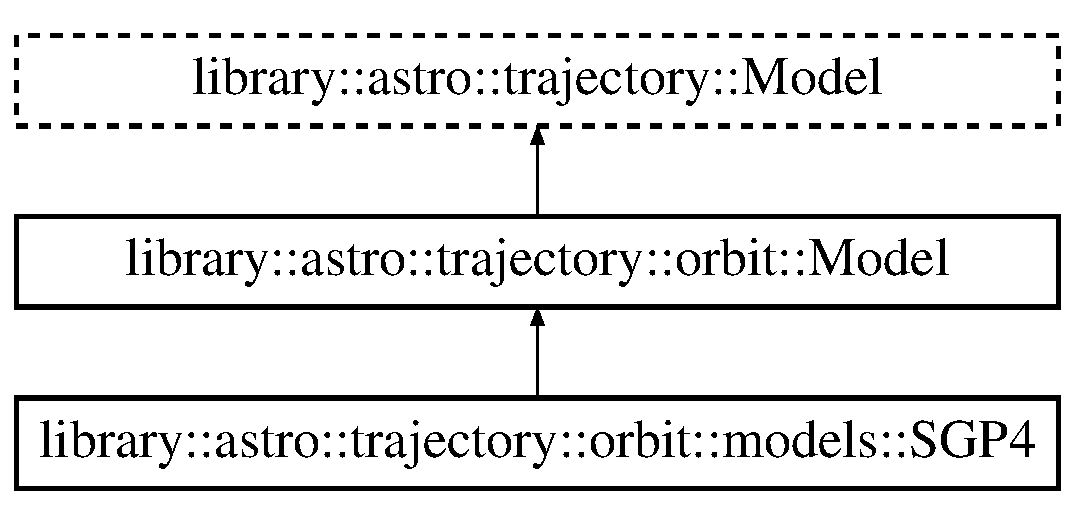
\includegraphics[height=3.000000cm]{classlibrary_1_1astro_1_1trajectory_1_1orbit_1_1models_1_1_s_g_p4}
\end{center}
\end{figure}
\subsection*{Public Member Functions}
\begin{DoxyCompactItemize}
\item 
\hyperlink{classlibrary_1_1astro_1_1trajectory_1_1orbit_1_1models_1_1_s_g_p4_aeb4f0869431bf4c65d8edaff53ae6ece}{S\+G\+P4} (const \hyperlink{classlibrary_1_1astro_1_1trajectory_1_1orbit_1_1models_1_1sgp4_1_1_t_l_e}{T\+LE} \&a\+Tle)
\item 
\hyperlink{classlibrary_1_1astro_1_1trajectory_1_1orbit_1_1models_1_1_s_g_p4_a8369d666690d2d83840eb9cd6456865e}{S\+G\+P4} (const \hyperlink{classlibrary_1_1astro_1_1trajectory_1_1orbit_1_1models_1_1_s_g_p4}{S\+G\+P4} \&a\+S\+G\+P4\+Model)
\item 
\hyperlink{classlibrary_1_1astro_1_1trajectory_1_1orbit_1_1models_1_1_s_g_p4_a317b4bca86822147ef5b71f8dea4f910}{$\sim$\+S\+G\+P4} ()
\item 
\hyperlink{classlibrary_1_1astro_1_1trajectory_1_1orbit_1_1models_1_1_s_g_p4}{S\+G\+P4} \& \hyperlink{classlibrary_1_1astro_1_1trajectory_1_1orbit_1_1models_1_1_s_g_p4_a44ff4ee45fa5becbb65cb9750ab2075f}{operator=} (const \hyperlink{classlibrary_1_1astro_1_1trajectory_1_1orbit_1_1models_1_1_s_g_p4}{S\+G\+P4} \&a\+S\+G\+P4\+Model)
\item 
virtual \hyperlink{classlibrary_1_1astro_1_1trajectory_1_1orbit_1_1models_1_1_s_g_p4}{S\+G\+P4} $\ast$ \hyperlink{classlibrary_1_1astro_1_1trajectory_1_1orbit_1_1models_1_1_s_g_p4_afa3add6c6855ac1da5632b17986dca02}{clone} () const override
\item 
bool \hyperlink{classlibrary_1_1astro_1_1trajectory_1_1orbit_1_1models_1_1_s_g_p4_af41acfeaec0d9896f15683ed20baf479}{operator==} (const \hyperlink{classlibrary_1_1astro_1_1trajectory_1_1orbit_1_1models_1_1_s_g_p4}{S\+G\+P4} \&a\+S\+G\+P4\+Model) const
\item 
bool \hyperlink{classlibrary_1_1astro_1_1trajectory_1_1orbit_1_1models_1_1_s_g_p4_a7efaabc3ed948705fdecf07a13fb104c}{operator!=} (const \hyperlink{classlibrary_1_1astro_1_1trajectory_1_1orbit_1_1models_1_1_s_g_p4}{S\+G\+P4} \&a\+S\+G\+P4\+Model) const
\item 
virtual bool \hyperlink{classlibrary_1_1astro_1_1trajectory_1_1orbit_1_1models_1_1_s_g_p4_a2d70ef4601e453156a430115e11ce8d7}{is\+Defined} () const override
\item 
\hyperlink{classlibrary_1_1astro_1_1trajectory_1_1orbit_1_1models_1_1sgp4_1_1_t_l_e}{T\+LE} \hyperlink{classlibrary_1_1astro_1_1trajectory_1_1orbit_1_1models_1_1_s_g_p4_a45a7bfb2099d304436898113706e1000}{get\+Tle} () const
\item 
virtual Instant \hyperlink{classlibrary_1_1astro_1_1trajectory_1_1orbit_1_1models_1_1_s_g_p4_a44439cf23b0d6d7b726b5b9c8784b5c1}{get\+Epoch} () const override
\item 
virtual Integer \hyperlink{classlibrary_1_1astro_1_1trajectory_1_1orbit_1_1models_1_1_s_g_p4_ac4b0a82cff7908a0192b7e2db3107f13}{get\+Revolution\+Number\+At\+Epoch} () const override
\item 
virtual \hyperlink{classlibrary_1_1astro_1_1trajectory_1_1_state}{State} \hyperlink{classlibrary_1_1astro_1_1trajectory_1_1orbit_1_1models_1_1_s_g_p4_a5d94d349c464f7313017c795a9346084}{calculate\+State\+At} (const Instant \&an\+Instant) const override
\item 
virtual Integer \hyperlink{classlibrary_1_1astro_1_1trajectory_1_1orbit_1_1models_1_1_s_g_p4_af1591139c936dd0c696972e5cb461009}{calculate\+Revolution\+Number\+At} (const Instant \&an\+Instant) const override
\item 
virtual void \hyperlink{classlibrary_1_1astro_1_1trajectory_1_1orbit_1_1models_1_1_s_g_p4_aca7d5615c14d59338506fb13630cd535}{print} (std\+::ostream \&an\+Output\+Stream, bool display\+Decorator=true) const override
\end{DoxyCompactItemize}
\subsection*{Protected Member Functions}
\begin{DoxyCompactItemize}
\item 
virtual bool \hyperlink{classlibrary_1_1astro_1_1trajectory_1_1orbit_1_1models_1_1_s_g_p4_a6210273bf78e8b98b310999a09d89cc4}{operator==} (const \hyperlink{classlibrary_1_1astro_1_1trajectory_1_1_model}{trajectory\+::\+Model} \&a\+Model) const override
\item 
virtual bool \hyperlink{classlibrary_1_1astro_1_1trajectory_1_1orbit_1_1models_1_1_s_g_p4_addbc5d1289986a6f89da00a21d4ab8e6}{operator!=} (const \hyperlink{classlibrary_1_1astro_1_1trajectory_1_1_model}{trajectory\+::\+Model} \&a\+Model) const override
\end{DoxyCompactItemize}
\subsection*{Friends}
\begin{DoxyCompactItemize}
\item 
std\+::ostream \& \hyperlink{classlibrary_1_1astro_1_1trajectory_1_1orbit_1_1models_1_1_s_g_p4_a44bd6a41f5d1be384d07b897785529f1}{operator$<$$<$} (std\+::ostream \&an\+Output\+Stream, const \hyperlink{classlibrary_1_1astro_1_1trajectory_1_1orbit_1_1models_1_1_s_g_p4}{S\+G\+P4} \&a\+S\+G\+P4\+Model)
\end{DoxyCompactItemize}


\subsection{Constructor \& Destructor Documentation}
\mbox{\Hypertarget{classlibrary_1_1astro_1_1trajectory_1_1orbit_1_1models_1_1_s_g_p4_aeb4f0869431bf4c65d8edaff53ae6ece}\label{classlibrary_1_1astro_1_1trajectory_1_1orbit_1_1models_1_1_s_g_p4_aeb4f0869431bf4c65d8edaff53ae6ece}} 
\index{library\+::astro\+::trajectory\+::orbit\+::models\+::\+S\+G\+P4@{library\+::astro\+::trajectory\+::orbit\+::models\+::\+S\+G\+P4}!S\+G\+P4@{S\+G\+P4}}
\index{S\+G\+P4@{S\+G\+P4}!library\+::astro\+::trajectory\+::orbit\+::models\+::\+S\+G\+P4@{library\+::astro\+::trajectory\+::orbit\+::models\+::\+S\+G\+P4}}
\subsubsection{\texorpdfstring{S\+G\+P4()}{SGP4()}\hspace{0.1cm}{\footnotesize\ttfamily [1/2]}}
{\footnotesize\ttfamily library\+::astro\+::trajectory\+::orbit\+::models\+::\+S\+G\+P4\+::\+S\+G\+P4 (\begin{DoxyParamCaption}\item[{const \hyperlink{classlibrary_1_1astro_1_1trajectory_1_1orbit_1_1models_1_1sgp4_1_1_t_l_e}{T\+LE} \&}]{a\+Tle }\end{DoxyParamCaption})}

\mbox{\Hypertarget{classlibrary_1_1astro_1_1trajectory_1_1orbit_1_1models_1_1_s_g_p4_a8369d666690d2d83840eb9cd6456865e}\label{classlibrary_1_1astro_1_1trajectory_1_1orbit_1_1models_1_1_s_g_p4_a8369d666690d2d83840eb9cd6456865e}} 
\index{library\+::astro\+::trajectory\+::orbit\+::models\+::\+S\+G\+P4@{library\+::astro\+::trajectory\+::orbit\+::models\+::\+S\+G\+P4}!S\+G\+P4@{S\+G\+P4}}
\index{S\+G\+P4@{S\+G\+P4}!library\+::astro\+::trajectory\+::orbit\+::models\+::\+S\+G\+P4@{library\+::astro\+::trajectory\+::orbit\+::models\+::\+S\+G\+P4}}
\subsubsection{\texorpdfstring{S\+G\+P4()}{SGP4()}\hspace{0.1cm}{\footnotesize\ttfamily [2/2]}}
{\footnotesize\ttfamily library\+::astro\+::trajectory\+::orbit\+::models\+::\+S\+G\+P4\+::\+S\+G\+P4 (\begin{DoxyParamCaption}\item[{const \hyperlink{classlibrary_1_1astro_1_1trajectory_1_1orbit_1_1models_1_1_s_g_p4}{S\+G\+P4} \&}]{a\+S\+G\+P4\+Model }\end{DoxyParamCaption})}

\mbox{\Hypertarget{classlibrary_1_1astro_1_1trajectory_1_1orbit_1_1models_1_1_s_g_p4_a317b4bca86822147ef5b71f8dea4f910}\label{classlibrary_1_1astro_1_1trajectory_1_1orbit_1_1models_1_1_s_g_p4_a317b4bca86822147ef5b71f8dea4f910}} 
\index{library\+::astro\+::trajectory\+::orbit\+::models\+::\+S\+G\+P4@{library\+::astro\+::trajectory\+::orbit\+::models\+::\+S\+G\+P4}!````~S\+G\+P4@{$\sim$\+S\+G\+P4}}
\index{````~S\+G\+P4@{$\sim$\+S\+G\+P4}!library\+::astro\+::trajectory\+::orbit\+::models\+::\+S\+G\+P4@{library\+::astro\+::trajectory\+::orbit\+::models\+::\+S\+G\+P4}}
\subsubsection{\texorpdfstring{$\sim$\+S\+G\+P4()}{~SGP4()}}
{\footnotesize\ttfamily library\+::astro\+::trajectory\+::orbit\+::models\+::\+S\+G\+P4\+::$\sim$\+S\+G\+P4 (\begin{DoxyParamCaption}{ }\end{DoxyParamCaption})}



\subsection{Member Function Documentation}
\mbox{\Hypertarget{classlibrary_1_1astro_1_1trajectory_1_1orbit_1_1models_1_1_s_g_p4_af1591139c936dd0c696972e5cb461009}\label{classlibrary_1_1astro_1_1trajectory_1_1orbit_1_1models_1_1_s_g_p4_af1591139c936dd0c696972e5cb461009}} 
\index{library\+::astro\+::trajectory\+::orbit\+::models\+::\+S\+G\+P4@{library\+::astro\+::trajectory\+::orbit\+::models\+::\+S\+G\+P4}!calculate\+Revolution\+Number\+At@{calculate\+Revolution\+Number\+At}}
\index{calculate\+Revolution\+Number\+At@{calculate\+Revolution\+Number\+At}!library\+::astro\+::trajectory\+::orbit\+::models\+::\+S\+G\+P4@{library\+::astro\+::trajectory\+::orbit\+::models\+::\+S\+G\+P4}}
\subsubsection{\texorpdfstring{calculate\+Revolution\+Number\+At()}{calculateRevolutionNumberAt()}}
{\footnotesize\ttfamily Integer library\+::astro\+::trajectory\+::orbit\+::models\+::\+S\+G\+P4\+::calculate\+Revolution\+Number\+At (\begin{DoxyParamCaption}\item[{const Instant \&}]{an\+Instant }\end{DoxyParamCaption}) const\hspace{0.3cm}{\ttfamily [override]}, {\ttfamily [virtual]}}



Implements \hyperlink{classlibrary_1_1astro_1_1trajectory_1_1orbit_1_1_model_a6329db5556ed72aa8ad18515aeaefeab}{library\+::astro\+::trajectory\+::orbit\+::\+Model}.

\mbox{\Hypertarget{classlibrary_1_1astro_1_1trajectory_1_1orbit_1_1models_1_1_s_g_p4_a5d94d349c464f7313017c795a9346084}\label{classlibrary_1_1astro_1_1trajectory_1_1orbit_1_1models_1_1_s_g_p4_a5d94d349c464f7313017c795a9346084}} 
\index{library\+::astro\+::trajectory\+::orbit\+::models\+::\+S\+G\+P4@{library\+::astro\+::trajectory\+::orbit\+::models\+::\+S\+G\+P4}!calculate\+State\+At@{calculate\+State\+At}}
\index{calculate\+State\+At@{calculate\+State\+At}!library\+::astro\+::trajectory\+::orbit\+::models\+::\+S\+G\+P4@{library\+::astro\+::trajectory\+::orbit\+::models\+::\+S\+G\+P4}}
\subsubsection{\texorpdfstring{calculate\+State\+At()}{calculateStateAt()}}
{\footnotesize\ttfamily \hyperlink{classlibrary_1_1astro_1_1trajectory_1_1_state}{State} library\+::astro\+::trajectory\+::orbit\+::models\+::\+S\+G\+P4\+::calculate\+State\+At (\begin{DoxyParamCaption}\item[{const Instant \&}]{an\+Instant }\end{DoxyParamCaption}) const\hspace{0.3cm}{\ttfamily [override]}, {\ttfamily [virtual]}}



Implements \hyperlink{classlibrary_1_1astro_1_1trajectory_1_1orbit_1_1_model_a34198a504836b9779425da99d964d19c}{library\+::astro\+::trajectory\+::orbit\+::\+Model}.

\mbox{\Hypertarget{classlibrary_1_1astro_1_1trajectory_1_1orbit_1_1models_1_1_s_g_p4_afa3add6c6855ac1da5632b17986dca02}\label{classlibrary_1_1astro_1_1trajectory_1_1orbit_1_1models_1_1_s_g_p4_afa3add6c6855ac1da5632b17986dca02}} 
\index{library\+::astro\+::trajectory\+::orbit\+::models\+::\+S\+G\+P4@{library\+::astro\+::trajectory\+::orbit\+::models\+::\+S\+G\+P4}!clone@{clone}}
\index{clone@{clone}!library\+::astro\+::trajectory\+::orbit\+::models\+::\+S\+G\+P4@{library\+::astro\+::trajectory\+::orbit\+::models\+::\+S\+G\+P4}}
\subsubsection{\texorpdfstring{clone()}{clone()}}
{\footnotesize\ttfamily \hyperlink{classlibrary_1_1astro_1_1trajectory_1_1orbit_1_1models_1_1_s_g_p4}{S\+G\+P4} $\ast$ library\+::astro\+::trajectory\+::orbit\+::models\+::\+S\+G\+P4\+::clone (\begin{DoxyParamCaption}{ }\end{DoxyParamCaption}) const\hspace{0.3cm}{\ttfamily [override]}, {\ttfamily [virtual]}}



Implements \hyperlink{classlibrary_1_1astro_1_1trajectory_1_1orbit_1_1_model_a45d75e4d212a9bb01aa596eaeeae43ae}{library\+::astro\+::trajectory\+::orbit\+::\+Model}.

\mbox{\Hypertarget{classlibrary_1_1astro_1_1trajectory_1_1orbit_1_1models_1_1_s_g_p4_a44439cf23b0d6d7b726b5b9c8784b5c1}\label{classlibrary_1_1astro_1_1trajectory_1_1orbit_1_1models_1_1_s_g_p4_a44439cf23b0d6d7b726b5b9c8784b5c1}} 
\index{library\+::astro\+::trajectory\+::orbit\+::models\+::\+S\+G\+P4@{library\+::astro\+::trajectory\+::orbit\+::models\+::\+S\+G\+P4}!get\+Epoch@{get\+Epoch}}
\index{get\+Epoch@{get\+Epoch}!library\+::astro\+::trajectory\+::orbit\+::models\+::\+S\+G\+P4@{library\+::astro\+::trajectory\+::orbit\+::models\+::\+S\+G\+P4}}
\subsubsection{\texorpdfstring{get\+Epoch()}{getEpoch()}}
{\footnotesize\ttfamily Instant library\+::astro\+::trajectory\+::orbit\+::models\+::\+S\+G\+P4\+::get\+Epoch (\begin{DoxyParamCaption}{ }\end{DoxyParamCaption}) const\hspace{0.3cm}{\ttfamily [override]}, {\ttfamily [virtual]}}



Implements \hyperlink{classlibrary_1_1astro_1_1trajectory_1_1orbit_1_1_model_acdec7ed6eed001c2ab4ac5442699a316}{library\+::astro\+::trajectory\+::orbit\+::\+Model}.

\mbox{\Hypertarget{classlibrary_1_1astro_1_1trajectory_1_1orbit_1_1models_1_1_s_g_p4_ac4b0a82cff7908a0192b7e2db3107f13}\label{classlibrary_1_1astro_1_1trajectory_1_1orbit_1_1models_1_1_s_g_p4_ac4b0a82cff7908a0192b7e2db3107f13}} 
\index{library\+::astro\+::trajectory\+::orbit\+::models\+::\+S\+G\+P4@{library\+::astro\+::trajectory\+::orbit\+::models\+::\+S\+G\+P4}!get\+Revolution\+Number\+At\+Epoch@{get\+Revolution\+Number\+At\+Epoch}}
\index{get\+Revolution\+Number\+At\+Epoch@{get\+Revolution\+Number\+At\+Epoch}!library\+::astro\+::trajectory\+::orbit\+::models\+::\+S\+G\+P4@{library\+::astro\+::trajectory\+::orbit\+::models\+::\+S\+G\+P4}}
\subsubsection{\texorpdfstring{get\+Revolution\+Number\+At\+Epoch()}{getRevolutionNumberAtEpoch()}}
{\footnotesize\ttfamily Integer library\+::astro\+::trajectory\+::orbit\+::models\+::\+S\+G\+P4\+::get\+Revolution\+Number\+At\+Epoch (\begin{DoxyParamCaption}{ }\end{DoxyParamCaption}) const\hspace{0.3cm}{\ttfamily [override]}, {\ttfamily [virtual]}}



Implements \hyperlink{classlibrary_1_1astro_1_1trajectory_1_1orbit_1_1_model_a940f5e266feb90ee8264d4c7a8a883f3}{library\+::astro\+::trajectory\+::orbit\+::\+Model}.

\mbox{\Hypertarget{classlibrary_1_1astro_1_1trajectory_1_1orbit_1_1models_1_1_s_g_p4_a45a7bfb2099d304436898113706e1000}\label{classlibrary_1_1astro_1_1trajectory_1_1orbit_1_1models_1_1_s_g_p4_a45a7bfb2099d304436898113706e1000}} 
\index{library\+::astro\+::trajectory\+::orbit\+::models\+::\+S\+G\+P4@{library\+::astro\+::trajectory\+::orbit\+::models\+::\+S\+G\+P4}!get\+Tle@{get\+Tle}}
\index{get\+Tle@{get\+Tle}!library\+::astro\+::trajectory\+::orbit\+::models\+::\+S\+G\+P4@{library\+::astro\+::trajectory\+::orbit\+::models\+::\+S\+G\+P4}}
\subsubsection{\texorpdfstring{get\+Tle()}{getTle()}}
{\footnotesize\ttfamily \hyperlink{classlibrary_1_1astro_1_1trajectory_1_1orbit_1_1models_1_1sgp4_1_1_t_l_e}{T\+LE} library\+::astro\+::trajectory\+::orbit\+::models\+::\+S\+G\+P4\+::get\+Tle (\begin{DoxyParamCaption}{ }\end{DoxyParamCaption}) const}

\mbox{\Hypertarget{classlibrary_1_1astro_1_1trajectory_1_1orbit_1_1models_1_1_s_g_p4_a2d70ef4601e453156a430115e11ce8d7}\label{classlibrary_1_1astro_1_1trajectory_1_1orbit_1_1models_1_1_s_g_p4_a2d70ef4601e453156a430115e11ce8d7}} 
\index{library\+::astro\+::trajectory\+::orbit\+::models\+::\+S\+G\+P4@{library\+::astro\+::trajectory\+::orbit\+::models\+::\+S\+G\+P4}!is\+Defined@{is\+Defined}}
\index{is\+Defined@{is\+Defined}!library\+::astro\+::trajectory\+::orbit\+::models\+::\+S\+G\+P4@{library\+::astro\+::trajectory\+::orbit\+::models\+::\+S\+G\+P4}}
\subsubsection{\texorpdfstring{is\+Defined()}{isDefined()}}
{\footnotesize\ttfamily bool library\+::astro\+::trajectory\+::orbit\+::models\+::\+S\+G\+P4\+::is\+Defined (\begin{DoxyParamCaption}{ }\end{DoxyParamCaption}) const\hspace{0.3cm}{\ttfamily [override]}, {\ttfamily [virtual]}}



Implements \hyperlink{classlibrary_1_1astro_1_1trajectory_1_1orbit_1_1_model_a518785603421d259e427bd0a6ee5e787}{library\+::astro\+::trajectory\+::orbit\+::\+Model}.

\mbox{\Hypertarget{classlibrary_1_1astro_1_1trajectory_1_1orbit_1_1models_1_1_s_g_p4_a7efaabc3ed948705fdecf07a13fb104c}\label{classlibrary_1_1astro_1_1trajectory_1_1orbit_1_1models_1_1_s_g_p4_a7efaabc3ed948705fdecf07a13fb104c}} 
\index{library\+::astro\+::trajectory\+::orbit\+::models\+::\+S\+G\+P4@{library\+::astro\+::trajectory\+::orbit\+::models\+::\+S\+G\+P4}!operator"!=@{operator"!=}}
\index{operator"!=@{operator"!=}!library\+::astro\+::trajectory\+::orbit\+::models\+::\+S\+G\+P4@{library\+::astro\+::trajectory\+::orbit\+::models\+::\+S\+G\+P4}}
\subsubsection{\texorpdfstring{operator"!=()}{operator!=()}\hspace{0.1cm}{\footnotesize\ttfamily [1/2]}}
{\footnotesize\ttfamily bool library\+::astro\+::trajectory\+::orbit\+::models\+::\+S\+G\+P4\+::operator!= (\begin{DoxyParamCaption}\item[{const \hyperlink{classlibrary_1_1astro_1_1trajectory_1_1orbit_1_1models_1_1_s_g_p4}{S\+G\+P4} \&}]{a\+S\+G\+P4\+Model }\end{DoxyParamCaption}) const}

\mbox{\Hypertarget{classlibrary_1_1astro_1_1trajectory_1_1orbit_1_1models_1_1_s_g_p4_addbc5d1289986a6f89da00a21d4ab8e6}\label{classlibrary_1_1astro_1_1trajectory_1_1orbit_1_1models_1_1_s_g_p4_addbc5d1289986a6f89da00a21d4ab8e6}} 
\index{library\+::astro\+::trajectory\+::orbit\+::models\+::\+S\+G\+P4@{library\+::astro\+::trajectory\+::orbit\+::models\+::\+S\+G\+P4}!operator"!=@{operator"!=}}
\index{operator"!=@{operator"!=}!library\+::astro\+::trajectory\+::orbit\+::models\+::\+S\+G\+P4@{library\+::astro\+::trajectory\+::orbit\+::models\+::\+S\+G\+P4}}
\subsubsection{\texorpdfstring{operator"!=()}{operator!=()}\hspace{0.1cm}{\footnotesize\ttfamily [2/2]}}
{\footnotesize\ttfamily bool library\+::astro\+::trajectory\+::orbit\+::models\+::\+S\+G\+P4\+::operator!= (\begin{DoxyParamCaption}\item[{const \hyperlink{classlibrary_1_1astro_1_1trajectory_1_1_model}{trajectory\+::\+Model} \&}]{a\+Model }\end{DoxyParamCaption}) const\hspace{0.3cm}{\ttfamily [override]}, {\ttfamily [protected]}, {\ttfamily [virtual]}}



Implements \hyperlink{classlibrary_1_1astro_1_1trajectory_1_1_model_a476c234f5fca1eb75f64f5a96fd83c61}{library\+::astro\+::trajectory\+::\+Model}.

\mbox{\Hypertarget{classlibrary_1_1astro_1_1trajectory_1_1orbit_1_1models_1_1_s_g_p4_a44ff4ee45fa5becbb65cb9750ab2075f}\label{classlibrary_1_1astro_1_1trajectory_1_1orbit_1_1models_1_1_s_g_p4_a44ff4ee45fa5becbb65cb9750ab2075f}} 
\index{library\+::astro\+::trajectory\+::orbit\+::models\+::\+S\+G\+P4@{library\+::astro\+::trajectory\+::orbit\+::models\+::\+S\+G\+P4}!operator=@{operator=}}
\index{operator=@{operator=}!library\+::astro\+::trajectory\+::orbit\+::models\+::\+S\+G\+P4@{library\+::astro\+::trajectory\+::orbit\+::models\+::\+S\+G\+P4}}
\subsubsection{\texorpdfstring{operator=()}{operator=()}}
{\footnotesize\ttfamily \hyperlink{classlibrary_1_1astro_1_1trajectory_1_1orbit_1_1models_1_1_s_g_p4}{S\+G\+P4} \& library\+::astro\+::trajectory\+::orbit\+::models\+::\+S\+G\+P4\+::operator= (\begin{DoxyParamCaption}\item[{const \hyperlink{classlibrary_1_1astro_1_1trajectory_1_1orbit_1_1models_1_1_s_g_p4}{S\+G\+P4} \&}]{a\+S\+G\+P4\+Model }\end{DoxyParamCaption})}

\mbox{\Hypertarget{classlibrary_1_1astro_1_1trajectory_1_1orbit_1_1models_1_1_s_g_p4_af41acfeaec0d9896f15683ed20baf479}\label{classlibrary_1_1astro_1_1trajectory_1_1orbit_1_1models_1_1_s_g_p4_af41acfeaec0d9896f15683ed20baf479}} 
\index{library\+::astro\+::trajectory\+::orbit\+::models\+::\+S\+G\+P4@{library\+::astro\+::trajectory\+::orbit\+::models\+::\+S\+G\+P4}!operator==@{operator==}}
\index{operator==@{operator==}!library\+::astro\+::trajectory\+::orbit\+::models\+::\+S\+G\+P4@{library\+::astro\+::trajectory\+::orbit\+::models\+::\+S\+G\+P4}}
\subsubsection{\texorpdfstring{operator==()}{operator==()}\hspace{0.1cm}{\footnotesize\ttfamily [1/2]}}
{\footnotesize\ttfamily bool library\+::astro\+::trajectory\+::orbit\+::models\+::\+S\+G\+P4\+::operator== (\begin{DoxyParamCaption}\item[{const \hyperlink{classlibrary_1_1astro_1_1trajectory_1_1orbit_1_1models_1_1_s_g_p4}{S\+G\+P4} \&}]{a\+S\+G\+P4\+Model }\end{DoxyParamCaption}) const}

\mbox{\Hypertarget{classlibrary_1_1astro_1_1trajectory_1_1orbit_1_1models_1_1_s_g_p4_a6210273bf78e8b98b310999a09d89cc4}\label{classlibrary_1_1astro_1_1trajectory_1_1orbit_1_1models_1_1_s_g_p4_a6210273bf78e8b98b310999a09d89cc4}} 
\index{library\+::astro\+::trajectory\+::orbit\+::models\+::\+S\+G\+P4@{library\+::astro\+::trajectory\+::orbit\+::models\+::\+S\+G\+P4}!operator==@{operator==}}
\index{operator==@{operator==}!library\+::astro\+::trajectory\+::orbit\+::models\+::\+S\+G\+P4@{library\+::astro\+::trajectory\+::orbit\+::models\+::\+S\+G\+P4}}
\subsubsection{\texorpdfstring{operator==()}{operator==()}\hspace{0.1cm}{\footnotesize\ttfamily [2/2]}}
{\footnotesize\ttfamily bool library\+::astro\+::trajectory\+::orbit\+::models\+::\+S\+G\+P4\+::operator== (\begin{DoxyParamCaption}\item[{const \hyperlink{classlibrary_1_1astro_1_1trajectory_1_1_model}{trajectory\+::\+Model} \&}]{a\+Model }\end{DoxyParamCaption}) const\hspace{0.3cm}{\ttfamily [override]}, {\ttfamily [protected]}, {\ttfamily [virtual]}}



Implements \hyperlink{classlibrary_1_1astro_1_1trajectory_1_1_model_a83c52eb23e8feea58d600c87700ed923}{library\+::astro\+::trajectory\+::\+Model}.

\mbox{\Hypertarget{classlibrary_1_1astro_1_1trajectory_1_1orbit_1_1models_1_1_s_g_p4_aca7d5615c14d59338506fb13630cd535}\label{classlibrary_1_1astro_1_1trajectory_1_1orbit_1_1models_1_1_s_g_p4_aca7d5615c14d59338506fb13630cd535}} 
\index{library\+::astro\+::trajectory\+::orbit\+::models\+::\+S\+G\+P4@{library\+::astro\+::trajectory\+::orbit\+::models\+::\+S\+G\+P4}!print@{print}}
\index{print@{print}!library\+::astro\+::trajectory\+::orbit\+::models\+::\+S\+G\+P4@{library\+::astro\+::trajectory\+::orbit\+::models\+::\+S\+G\+P4}}
\subsubsection{\texorpdfstring{print()}{print()}}
{\footnotesize\ttfamily void library\+::astro\+::trajectory\+::orbit\+::models\+::\+S\+G\+P4\+::print (\begin{DoxyParamCaption}\item[{std\+::ostream \&}]{an\+Output\+Stream,  }\item[{bool}]{display\+Decorator = {\ttfamily true} }\end{DoxyParamCaption}) const\hspace{0.3cm}{\ttfamily [override]}, {\ttfamily [virtual]}}



Implements \hyperlink{classlibrary_1_1astro_1_1trajectory_1_1orbit_1_1_model_abd4fb7604274cc8b3589a445db64e98c}{library\+::astro\+::trajectory\+::orbit\+::\+Model}.



\subsection{Friends And Related Function Documentation}
\mbox{\Hypertarget{classlibrary_1_1astro_1_1trajectory_1_1orbit_1_1models_1_1_s_g_p4_a44bd6a41f5d1be384d07b897785529f1}\label{classlibrary_1_1astro_1_1trajectory_1_1orbit_1_1models_1_1_s_g_p4_a44bd6a41f5d1be384d07b897785529f1}} 
\index{library\+::astro\+::trajectory\+::orbit\+::models\+::\+S\+G\+P4@{library\+::astro\+::trajectory\+::orbit\+::models\+::\+S\+G\+P4}!operator$<$$<$@{operator$<$$<$}}
\index{operator$<$$<$@{operator$<$$<$}!library\+::astro\+::trajectory\+::orbit\+::models\+::\+S\+G\+P4@{library\+::astro\+::trajectory\+::orbit\+::models\+::\+S\+G\+P4}}
\subsubsection{\texorpdfstring{operator$<$$<$}{operator<<}}
{\footnotesize\ttfamily std\+::ostream\& operator$<$$<$ (\begin{DoxyParamCaption}\item[{std\+::ostream \&}]{an\+Output\+Stream,  }\item[{const \hyperlink{classlibrary_1_1astro_1_1trajectory_1_1orbit_1_1models_1_1_s_g_p4}{S\+G\+P4} \&}]{a\+S\+G\+P4\+Model }\end{DoxyParamCaption})\hspace{0.3cm}{\ttfamily [friend]}}



The documentation for this class was generated from the following files\+:\begin{DoxyCompactItemize}
\item 
include/\+Library/\+Astrodynamics/\+Trajectory/\+Orbit/\+Models/\hyperlink{_s_g_p4_8hpp}{S\+G\+P4.\+hpp}\item 
src/\+Library/\+Astrodynamics/\+Trajectory/\+Orbit/\+Models/\hyperlink{_s_g_p4_8cpp}{S\+G\+P4.\+cpp}\end{DoxyCompactItemize}

\hypertarget{classlibrary_1_1astro_1_1trajectory_1_1_state}{}\section{library\+:\+:astro\+:\+:trajectory\+:\+:State Class Reference}
\label{classlibrary_1_1astro_1_1trajectory_1_1_state}\index{library\+::astro\+::trajectory\+::\+State@{library\+::astro\+::trajectory\+::\+State}}


\hyperlink{classlibrary_1_1astro_1_1_trajectory}{Trajectory} state.  




{\ttfamily \#include $<$State.\+hpp$>$}

\subsection*{Public Member Functions}
\begin{DoxyCompactItemize}
\item 
\hyperlink{classlibrary_1_1astro_1_1trajectory_1_1_state_ada1cbf99efb7e85f0a1f9664868b20f5}{State} (const Instant \&an\+Instant, const Position \&a\+Position, const Velocity \&a\+Velocity)
\item 
bool \hyperlink{classlibrary_1_1astro_1_1trajectory_1_1_state_a3b5c3a4279b3c0659cdb8d26a2b4202c}{operator==} (const \hyperlink{classlibrary_1_1astro_1_1trajectory_1_1_state}{State} \&a\+State) const
\item 
bool \hyperlink{classlibrary_1_1astro_1_1trajectory_1_1_state_aa3ceea8c71e864839693a4aa7d3e93c2}{operator!=} (const \hyperlink{classlibrary_1_1astro_1_1trajectory_1_1_state}{State} \&a\+State) const
\item 
bool \hyperlink{classlibrary_1_1astro_1_1trajectory_1_1_state_a62bb004d41468603c0dc9b17d505158e}{is\+Defined} () const
\item 
const Instant \& \hyperlink{classlibrary_1_1astro_1_1trajectory_1_1_state_ae51674051753513c7657e154331be976}{access\+Instant} () const
\item 
const Position \& \hyperlink{classlibrary_1_1astro_1_1trajectory_1_1_state_ab0751200244a8b741fd67a1bfb47ad4d}{access\+Position} () const
\item 
const Velocity \& \hyperlink{classlibrary_1_1astro_1_1trajectory_1_1_state_ae81763c334c3bd69595917a94c60d9d5}{access\+Velocity} () const
\item 
Instant \hyperlink{classlibrary_1_1astro_1_1trajectory_1_1_state_a7c053801b20c9501156720253c6c1707}{get\+Instant} () const
\item 
Position \hyperlink{classlibrary_1_1astro_1_1trajectory_1_1_state_aa75125aa07bc506bfaca1e2fcfbab8a8}{get\+Position} () const
\item 
Velocity \hyperlink{classlibrary_1_1astro_1_1trajectory_1_1_state_a778acffd0f76d9409e8de7920893439a}{get\+Velocity} () const
\item 
\hyperlink{classlibrary_1_1astro_1_1trajectory_1_1_state}{State} \hyperlink{classlibrary_1_1astro_1_1trajectory_1_1_state_aeef0e18554b9b9ac67a15aed7c5e59fb}{in\+Frame} (const Shared$<$ const Frame $>$ \&a\+Frame\+S\+Ptr) const
\end{DoxyCompactItemize}
\subsection*{Static Public Member Functions}
\begin{DoxyCompactItemize}
\item 
static \hyperlink{classlibrary_1_1astro_1_1trajectory_1_1_state}{State} \hyperlink{classlibrary_1_1astro_1_1trajectory_1_1_state_a1de5d9ea3f03d975b989fd519d447be7}{Undefined} ()
\end{DoxyCompactItemize}
\subsection*{Friends}
\begin{DoxyCompactItemize}
\item 
std\+::ostream \& \hyperlink{classlibrary_1_1astro_1_1trajectory_1_1_state_abba03f039f2534d691a1dc28426e8b89}{operator$<$$<$} (std\+::ostream \&an\+Output\+Stream, const \hyperlink{classlibrary_1_1astro_1_1trajectory_1_1_state}{State} \&a\+State)
\end{DoxyCompactItemize}


\subsection{Detailed Description}
\hyperlink{classlibrary_1_1astro_1_1_trajectory}{Trajectory} state. 

\subsection{Constructor \& Destructor Documentation}
\mbox{\Hypertarget{classlibrary_1_1astro_1_1trajectory_1_1_state_ada1cbf99efb7e85f0a1f9664868b20f5}\label{classlibrary_1_1astro_1_1trajectory_1_1_state_ada1cbf99efb7e85f0a1f9664868b20f5}} 
\index{library\+::astro\+::trajectory\+::\+State@{library\+::astro\+::trajectory\+::\+State}!State@{State}}
\index{State@{State}!library\+::astro\+::trajectory\+::\+State@{library\+::astro\+::trajectory\+::\+State}}
\subsubsection{\texorpdfstring{State()}{State()}}
{\footnotesize\ttfamily library\+::astro\+::trajectory\+::\+State\+::\+State (\begin{DoxyParamCaption}\item[{const Instant \&}]{an\+Instant,  }\item[{const Position \&}]{a\+Position,  }\item[{const Velocity \&}]{a\+Velocity }\end{DoxyParamCaption})}



\subsection{Member Function Documentation}
\mbox{\Hypertarget{classlibrary_1_1astro_1_1trajectory_1_1_state_ae51674051753513c7657e154331be976}\label{classlibrary_1_1astro_1_1trajectory_1_1_state_ae51674051753513c7657e154331be976}} 
\index{library\+::astro\+::trajectory\+::\+State@{library\+::astro\+::trajectory\+::\+State}!access\+Instant@{access\+Instant}}
\index{access\+Instant@{access\+Instant}!library\+::astro\+::trajectory\+::\+State@{library\+::astro\+::trajectory\+::\+State}}
\subsubsection{\texorpdfstring{access\+Instant()}{accessInstant()}}
{\footnotesize\ttfamily const Instant \& library\+::astro\+::trajectory\+::\+State\+::access\+Instant (\begin{DoxyParamCaption}{ }\end{DoxyParamCaption}) const}

\mbox{\Hypertarget{classlibrary_1_1astro_1_1trajectory_1_1_state_ab0751200244a8b741fd67a1bfb47ad4d}\label{classlibrary_1_1astro_1_1trajectory_1_1_state_ab0751200244a8b741fd67a1bfb47ad4d}} 
\index{library\+::astro\+::trajectory\+::\+State@{library\+::astro\+::trajectory\+::\+State}!access\+Position@{access\+Position}}
\index{access\+Position@{access\+Position}!library\+::astro\+::trajectory\+::\+State@{library\+::astro\+::trajectory\+::\+State}}
\subsubsection{\texorpdfstring{access\+Position()}{accessPosition()}}
{\footnotesize\ttfamily const Position \& library\+::astro\+::trajectory\+::\+State\+::access\+Position (\begin{DoxyParamCaption}{ }\end{DoxyParamCaption}) const}

\mbox{\Hypertarget{classlibrary_1_1astro_1_1trajectory_1_1_state_ae81763c334c3bd69595917a94c60d9d5}\label{classlibrary_1_1astro_1_1trajectory_1_1_state_ae81763c334c3bd69595917a94c60d9d5}} 
\index{library\+::astro\+::trajectory\+::\+State@{library\+::astro\+::trajectory\+::\+State}!access\+Velocity@{access\+Velocity}}
\index{access\+Velocity@{access\+Velocity}!library\+::astro\+::trajectory\+::\+State@{library\+::astro\+::trajectory\+::\+State}}
\subsubsection{\texorpdfstring{access\+Velocity()}{accessVelocity()}}
{\footnotesize\ttfamily const Velocity \& library\+::astro\+::trajectory\+::\+State\+::access\+Velocity (\begin{DoxyParamCaption}{ }\end{DoxyParamCaption}) const}

\mbox{\Hypertarget{classlibrary_1_1astro_1_1trajectory_1_1_state_a7c053801b20c9501156720253c6c1707}\label{classlibrary_1_1astro_1_1trajectory_1_1_state_a7c053801b20c9501156720253c6c1707}} 
\index{library\+::astro\+::trajectory\+::\+State@{library\+::astro\+::trajectory\+::\+State}!get\+Instant@{get\+Instant}}
\index{get\+Instant@{get\+Instant}!library\+::astro\+::trajectory\+::\+State@{library\+::astro\+::trajectory\+::\+State}}
\subsubsection{\texorpdfstring{get\+Instant()}{getInstant()}}
{\footnotesize\ttfamily Instant library\+::astro\+::trajectory\+::\+State\+::get\+Instant (\begin{DoxyParamCaption}{ }\end{DoxyParamCaption}) const}

\mbox{\Hypertarget{classlibrary_1_1astro_1_1trajectory_1_1_state_aa75125aa07bc506bfaca1e2fcfbab8a8}\label{classlibrary_1_1astro_1_1trajectory_1_1_state_aa75125aa07bc506bfaca1e2fcfbab8a8}} 
\index{library\+::astro\+::trajectory\+::\+State@{library\+::astro\+::trajectory\+::\+State}!get\+Position@{get\+Position}}
\index{get\+Position@{get\+Position}!library\+::astro\+::trajectory\+::\+State@{library\+::astro\+::trajectory\+::\+State}}
\subsubsection{\texorpdfstring{get\+Position()}{getPosition()}}
{\footnotesize\ttfamily Position library\+::astro\+::trajectory\+::\+State\+::get\+Position (\begin{DoxyParamCaption}{ }\end{DoxyParamCaption}) const}

\mbox{\Hypertarget{classlibrary_1_1astro_1_1trajectory_1_1_state_a778acffd0f76d9409e8de7920893439a}\label{classlibrary_1_1astro_1_1trajectory_1_1_state_a778acffd0f76d9409e8de7920893439a}} 
\index{library\+::astro\+::trajectory\+::\+State@{library\+::astro\+::trajectory\+::\+State}!get\+Velocity@{get\+Velocity}}
\index{get\+Velocity@{get\+Velocity}!library\+::astro\+::trajectory\+::\+State@{library\+::astro\+::trajectory\+::\+State}}
\subsubsection{\texorpdfstring{get\+Velocity()}{getVelocity()}}
{\footnotesize\ttfamily Velocity library\+::astro\+::trajectory\+::\+State\+::get\+Velocity (\begin{DoxyParamCaption}{ }\end{DoxyParamCaption}) const}

\mbox{\Hypertarget{classlibrary_1_1astro_1_1trajectory_1_1_state_aeef0e18554b9b9ac67a15aed7c5e59fb}\label{classlibrary_1_1astro_1_1trajectory_1_1_state_aeef0e18554b9b9ac67a15aed7c5e59fb}} 
\index{library\+::astro\+::trajectory\+::\+State@{library\+::astro\+::trajectory\+::\+State}!in\+Frame@{in\+Frame}}
\index{in\+Frame@{in\+Frame}!library\+::astro\+::trajectory\+::\+State@{library\+::astro\+::trajectory\+::\+State}}
\subsubsection{\texorpdfstring{in\+Frame()}{inFrame()}}
{\footnotesize\ttfamily \hyperlink{classlibrary_1_1astro_1_1trajectory_1_1_state}{State} library\+::astro\+::trajectory\+::\+State\+::in\+Frame (\begin{DoxyParamCaption}\item[{const Shared$<$ const Frame $>$ \&}]{a\+Frame\+S\+Ptr }\end{DoxyParamCaption}) const}

\mbox{\Hypertarget{classlibrary_1_1astro_1_1trajectory_1_1_state_a62bb004d41468603c0dc9b17d505158e}\label{classlibrary_1_1astro_1_1trajectory_1_1_state_a62bb004d41468603c0dc9b17d505158e}} 
\index{library\+::astro\+::trajectory\+::\+State@{library\+::astro\+::trajectory\+::\+State}!is\+Defined@{is\+Defined}}
\index{is\+Defined@{is\+Defined}!library\+::astro\+::trajectory\+::\+State@{library\+::astro\+::trajectory\+::\+State}}
\subsubsection{\texorpdfstring{is\+Defined()}{isDefined()}}
{\footnotesize\ttfamily bool library\+::astro\+::trajectory\+::\+State\+::is\+Defined (\begin{DoxyParamCaption}{ }\end{DoxyParamCaption}) const}

\mbox{\Hypertarget{classlibrary_1_1astro_1_1trajectory_1_1_state_aa3ceea8c71e864839693a4aa7d3e93c2}\label{classlibrary_1_1astro_1_1trajectory_1_1_state_aa3ceea8c71e864839693a4aa7d3e93c2}} 
\index{library\+::astro\+::trajectory\+::\+State@{library\+::astro\+::trajectory\+::\+State}!operator"!=@{operator"!=}}
\index{operator"!=@{operator"!=}!library\+::astro\+::trajectory\+::\+State@{library\+::astro\+::trajectory\+::\+State}}
\subsubsection{\texorpdfstring{operator"!=()}{operator!=()}}
{\footnotesize\ttfamily bool library\+::astro\+::trajectory\+::\+State\+::operator!= (\begin{DoxyParamCaption}\item[{const \hyperlink{classlibrary_1_1astro_1_1trajectory_1_1_state}{State} \&}]{a\+State }\end{DoxyParamCaption}) const}

\mbox{\Hypertarget{classlibrary_1_1astro_1_1trajectory_1_1_state_a3b5c3a4279b3c0659cdb8d26a2b4202c}\label{classlibrary_1_1astro_1_1trajectory_1_1_state_a3b5c3a4279b3c0659cdb8d26a2b4202c}} 
\index{library\+::astro\+::trajectory\+::\+State@{library\+::astro\+::trajectory\+::\+State}!operator==@{operator==}}
\index{operator==@{operator==}!library\+::astro\+::trajectory\+::\+State@{library\+::astro\+::trajectory\+::\+State}}
\subsubsection{\texorpdfstring{operator==()}{operator==()}}
{\footnotesize\ttfamily bool library\+::astro\+::trajectory\+::\+State\+::operator== (\begin{DoxyParamCaption}\item[{const \hyperlink{classlibrary_1_1astro_1_1trajectory_1_1_state}{State} \&}]{a\+State }\end{DoxyParamCaption}) const}

\mbox{\Hypertarget{classlibrary_1_1astro_1_1trajectory_1_1_state_a1de5d9ea3f03d975b989fd519d447be7}\label{classlibrary_1_1astro_1_1trajectory_1_1_state_a1de5d9ea3f03d975b989fd519d447be7}} 
\index{library\+::astro\+::trajectory\+::\+State@{library\+::astro\+::trajectory\+::\+State}!Undefined@{Undefined}}
\index{Undefined@{Undefined}!library\+::astro\+::trajectory\+::\+State@{library\+::astro\+::trajectory\+::\+State}}
\subsubsection{\texorpdfstring{Undefined()}{Undefined()}}
{\footnotesize\ttfamily \hyperlink{classlibrary_1_1astro_1_1trajectory_1_1_state}{State} library\+::astro\+::trajectory\+::\+State\+::\+Undefined (\begin{DoxyParamCaption}{ }\end{DoxyParamCaption})\hspace{0.3cm}{\ttfamily [static]}}



\subsection{Friends And Related Function Documentation}
\mbox{\Hypertarget{classlibrary_1_1astro_1_1trajectory_1_1_state_abba03f039f2534d691a1dc28426e8b89}\label{classlibrary_1_1astro_1_1trajectory_1_1_state_abba03f039f2534d691a1dc28426e8b89}} 
\index{library\+::astro\+::trajectory\+::\+State@{library\+::astro\+::trajectory\+::\+State}!operator$<$$<$@{operator$<$$<$}}
\index{operator$<$$<$@{operator$<$$<$}!library\+::astro\+::trajectory\+::\+State@{library\+::astro\+::trajectory\+::\+State}}
\subsubsection{\texorpdfstring{operator$<$$<$}{operator<<}}
{\footnotesize\ttfamily std\+::ostream\& operator$<$$<$ (\begin{DoxyParamCaption}\item[{std\+::ostream \&}]{an\+Output\+Stream,  }\item[{const \hyperlink{classlibrary_1_1astro_1_1trajectory_1_1_state}{State} \&}]{a\+State }\end{DoxyParamCaption})\hspace{0.3cm}{\ttfamily [friend]}}



The documentation for this class was generated from the following files\+:\begin{DoxyCompactItemize}
\item 
include/\+Library/\+Astrodynamics/\+Trajectory/\hyperlink{_state_8hpp}{State.\+hpp}\item 
src/\+Library/\+Astrodynamics/\+Trajectory/\hyperlink{_state_8cpp}{State.\+cpp}\end{DoxyCompactItemize}

\hypertarget{classlibrary_1_1astro_1_1flight_1_1profile_1_1_state}{}\section{library\+:\+:astro\+:\+:flight\+:\+:profile\+:\+:State Class Reference}
\label{classlibrary_1_1astro_1_1flight_1_1profile_1_1_state}\index{library\+::astro\+::flight\+::profile\+::\+State@{library\+::astro\+::flight\+::profile\+::\+State}}


Spacecraft flight profile state.  




{\ttfamily \#include $<$State.\+hpp$>$}

\subsection*{Public Member Functions}
\begin{DoxyCompactItemize}
\item 
\hyperlink{classlibrary_1_1astro_1_1flight_1_1profile_1_1_state_a254a001f4c2ddc33684dbfdd4ee07194}{State} (const Instant \&an\+Instant, const Vector3d \&a\+Position, const Vector3d \&a\+Velocity, const Quaternion \&an\+Attitude, const Vector3d \&an\+Angular\+Velocity, const Shared$<$ const Frame $>$ \&a\+Reference\+Frame)
\item 
bool \hyperlink{classlibrary_1_1astro_1_1flight_1_1profile_1_1_state_af9508e4482013592c37e57173baea944}{operator==} (const \hyperlink{classlibrary_1_1astro_1_1flight_1_1profile_1_1_state}{State} \&a\+State) const
\item 
bool \hyperlink{classlibrary_1_1astro_1_1flight_1_1profile_1_1_state_a086731f12479cad3f2e505572fa67883}{operator!=} (const \hyperlink{classlibrary_1_1astro_1_1flight_1_1profile_1_1_state}{State} \&a\+State) const
\item 
bool \hyperlink{classlibrary_1_1astro_1_1flight_1_1profile_1_1_state_a1fceb93d0163b18666319c16aef6dd23}{is\+Defined} () const
\item 
const Instant \& \hyperlink{classlibrary_1_1astro_1_1flight_1_1profile_1_1_state_abc3c190e5bdceda1d7c15bb685edfcc9}{access\+Instant} () const
\item 
const Vector3d \& \hyperlink{classlibrary_1_1astro_1_1flight_1_1profile_1_1_state_a96a4a1054299c79d8aafdde3313a4116}{access\+Position} () const
\item 
const Vector3d \& \hyperlink{classlibrary_1_1astro_1_1flight_1_1profile_1_1_state_a849c6426b346b48465b3e24c2248a4d8}{access\+Velocity} () const
\item 
const Quaternion \& \hyperlink{classlibrary_1_1astro_1_1flight_1_1profile_1_1_state_ac82679e41392dde2137f0e15247c3227}{access\+Attitude} () const
\item 
const Vector3d \& \hyperlink{classlibrary_1_1astro_1_1flight_1_1profile_1_1_state_ac370e25be16830246a01df5e503ddedb}{access\+Angular\+Velocity} () const
\item 
Instant \hyperlink{classlibrary_1_1astro_1_1flight_1_1profile_1_1_state_abf0cb1f8403d99cb3e091fcf77997c91}{get\+Instant} () const
\item 
Vector3d \hyperlink{classlibrary_1_1astro_1_1flight_1_1profile_1_1_state_afaa3df4fd14876d51cd840e790f26b6f}{get\+Position} () const
\item 
Vector3d \hyperlink{classlibrary_1_1astro_1_1flight_1_1profile_1_1_state_a0da3770b1a85608524d29d7f4ddec557}{get\+Velocity} () const
\item 
Quaternion \hyperlink{classlibrary_1_1astro_1_1flight_1_1profile_1_1_state_a473831938892a97366ed5fb24b51e7be}{get\+Attitude} () const
\item 
Vector3d \hyperlink{classlibrary_1_1astro_1_1flight_1_1profile_1_1_state_ab228ee5983e7d1c1f93e534013f87b7d}{get\+Angular\+Velocity} () const
\item 
Shared$<$ const Frame $>$ \hyperlink{classlibrary_1_1astro_1_1flight_1_1profile_1_1_state_aa0de9fc4cfaf54134230e5e99f276fb4}{get\+Frame} () const
\item 
\hyperlink{classlibrary_1_1astro_1_1flight_1_1profile_1_1_state}{State} \hyperlink{classlibrary_1_1astro_1_1flight_1_1profile_1_1_state_a29ebd3fb92ad525b65782a904713b8ff}{in\+Frame} (const Shared$<$ const Frame $>$ \&a\+Frame\+S\+Ptr) const
\end{DoxyCompactItemize}
\subsection*{Static Public Member Functions}
\begin{DoxyCompactItemize}
\item 
static \hyperlink{classlibrary_1_1astro_1_1flight_1_1profile_1_1_state}{State} \hyperlink{classlibrary_1_1astro_1_1flight_1_1profile_1_1_state_a1ad05946cb00b3b26fd7b56e8f8bfe94}{Undefined} ()
\end{DoxyCompactItemize}
\subsection*{Friends}
\begin{DoxyCompactItemize}
\item 
std\+::ostream \& \hyperlink{classlibrary_1_1astro_1_1flight_1_1profile_1_1_state_abba03f039f2534d691a1dc28426e8b89}{operator$<$$<$} (std\+::ostream \&an\+Output\+Stream, const \hyperlink{classlibrary_1_1astro_1_1flight_1_1profile_1_1_state}{State} \&a\+State)
\end{DoxyCompactItemize}


\subsection{Detailed Description}
Spacecraft flight profile state. 

\subsection{Constructor \& Destructor Documentation}
\mbox{\Hypertarget{classlibrary_1_1astro_1_1flight_1_1profile_1_1_state_a254a001f4c2ddc33684dbfdd4ee07194}\label{classlibrary_1_1astro_1_1flight_1_1profile_1_1_state_a254a001f4c2ddc33684dbfdd4ee07194}} 
\index{library\+::astro\+::flight\+::profile\+::\+State@{library\+::astro\+::flight\+::profile\+::\+State}!State@{State}}
\index{State@{State}!library\+::astro\+::flight\+::profile\+::\+State@{library\+::astro\+::flight\+::profile\+::\+State}}
\subsubsection{\texorpdfstring{State()}{State()}}
{\footnotesize\ttfamily library\+::astro\+::flight\+::profile\+::\+State\+::\+State (\begin{DoxyParamCaption}\item[{const Instant \&}]{an\+Instant,  }\item[{const Vector3d \&}]{a\+Position,  }\item[{const Vector3d \&}]{a\+Velocity,  }\item[{const Quaternion \&}]{an\+Attitude,  }\item[{const Vector3d \&}]{an\+Angular\+Velocity,  }\item[{const Shared$<$ const Frame $>$ \&}]{a\+Reference\+Frame }\end{DoxyParamCaption})}



\subsection{Member Function Documentation}
\mbox{\Hypertarget{classlibrary_1_1astro_1_1flight_1_1profile_1_1_state_ac370e25be16830246a01df5e503ddedb}\label{classlibrary_1_1astro_1_1flight_1_1profile_1_1_state_ac370e25be16830246a01df5e503ddedb}} 
\index{library\+::astro\+::flight\+::profile\+::\+State@{library\+::astro\+::flight\+::profile\+::\+State}!access\+Angular\+Velocity@{access\+Angular\+Velocity}}
\index{access\+Angular\+Velocity@{access\+Angular\+Velocity}!library\+::astro\+::flight\+::profile\+::\+State@{library\+::astro\+::flight\+::profile\+::\+State}}
\subsubsection{\texorpdfstring{access\+Angular\+Velocity()}{accessAngularVelocity()}}
{\footnotesize\ttfamily const Vector3d \& library\+::astro\+::flight\+::profile\+::\+State\+::access\+Angular\+Velocity (\begin{DoxyParamCaption}{ }\end{DoxyParamCaption}) const}

\mbox{\Hypertarget{classlibrary_1_1astro_1_1flight_1_1profile_1_1_state_ac82679e41392dde2137f0e15247c3227}\label{classlibrary_1_1astro_1_1flight_1_1profile_1_1_state_ac82679e41392dde2137f0e15247c3227}} 
\index{library\+::astro\+::flight\+::profile\+::\+State@{library\+::astro\+::flight\+::profile\+::\+State}!access\+Attitude@{access\+Attitude}}
\index{access\+Attitude@{access\+Attitude}!library\+::astro\+::flight\+::profile\+::\+State@{library\+::astro\+::flight\+::profile\+::\+State}}
\subsubsection{\texorpdfstring{access\+Attitude()}{accessAttitude()}}
{\footnotesize\ttfamily const Quaternion \& library\+::astro\+::flight\+::profile\+::\+State\+::access\+Attitude (\begin{DoxyParamCaption}{ }\end{DoxyParamCaption}) const}

\mbox{\Hypertarget{classlibrary_1_1astro_1_1flight_1_1profile_1_1_state_abc3c190e5bdceda1d7c15bb685edfcc9}\label{classlibrary_1_1astro_1_1flight_1_1profile_1_1_state_abc3c190e5bdceda1d7c15bb685edfcc9}} 
\index{library\+::astro\+::flight\+::profile\+::\+State@{library\+::astro\+::flight\+::profile\+::\+State}!access\+Instant@{access\+Instant}}
\index{access\+Instant@{access\+Instant}!library\+::astro\+::flight\+::profile\+::\+State@{library\+::astro\+::flight\+::profile\+::\+State}}
\subsubsection{\texorpdfstring{access\+Instant()}{accessInstant()}}
{\footnotesize\ttfamily const Instant \& library\+::astro\+::flight\+::profile\+::\+State\+::access\+Instant (\begin{DoxyParamCaption}{ }\end{DoxyParamCaption}) const}

\mbox{\Hypertarget{classlibrary_1_1astro_1_1flight_1_1profile_1_1_state_a96a4a1054299c79d8aafdde3313a4116}\label{classlibrary_1_1astro_1_1flight_1_1profile_1_1_state_a96a4a1054299c79d8aafdde3313a4116}} 
\index{library\+::astro\+::flight\+::profile\+::\+State@{library\+::astro\+::flight\+::profile\+::\+State}!access\+Position@{access\+Position}}
\index{access\+Position@{access\+Position}!library\+::astro\+::flight\+::profile\+::\+State@{library\+::astro\+::flight\+::profile\+::\+State}}
\subsubsection{\texorpdfstring{access\+Position()}{accessPosition()}}
{\footnotesize\ttfamily const Vector3d \& library\+::astro\+::flight\+::profile\+::\+State\+::access\+Position (\begin{DoxyParamCaption}{ }\end{DoxyParamCaption}) const}

\mbox{\Hypertarget{classlibrary_1_1astro_1_1flight_1_1profile_1_1_state_a849c6426b346b48465b3e24c2248a4d8}\label{classlibrary_1_1astro_1_1flight_1_1profile_1_1_state_a849c6426b346b48465b3e24c2248a4d8}} 
\index{library\+::astro\+::flight\+::profile\+::\+State@{library\+::astro\+::flight\+::profile\+::\+State}!access\+Velocity@{access\+Velocity}}
\index{access\+Velocity@{access\+Velocity}!library\+::astro\+::flight\+::profile\+::\+State@{library\+::astro\+::flight\+::profile\+::\+State}}
\subsubsection{\texorpdfstring{access\+Velocity()}{accessVelocity()}}
{\footnotesize\ttfamily const Vector3d \& library\+::astro\+::flight\+::profile\+::\+State\+::access\+Velocity (\begin{DoxyParamCaption}{ }\end{DoxyParamCaption}) const}

\mbox{\Hypertarget{classlibrary_1_1astro_1_1flight_1_1profile_1_1_state_ab228ee5983e7d1c1f93e534013f87b7d}\label{classlibrary_1_1astro_1_1flight_1_1profile_1_1_state_ab228ee5983e7d1c1f93e534013f87b7d}} 
\index{library\+::astro\+::flight\+::profile\+::\+State@{library\+::astro\+::flight\+::profile\+::\+State}!get\+Angular\+Velocity@{get\+Angular\+Velocity}}
\index{get\+Angular\+Velocity@{get\+Angular\+Velocity}!library\+::astro\+::flight\+::profile\+::\+State@{library\+::astro\+::flight\+::profile\+::\+State}}
\subsubsection{\texorpdfstring{get\+Angular\+Velocity()}{getAngularVelocity()}}
{\footnotesize\ttfamily Vector3d library\+::astro\+::flight\+::profile\+::\+State\+::get\+Angular\+Velocity (\begin{DoxyParamCaption}{ }\end{DoxyParamCaption}) const}

\mbox{\Hypertarget{classlibrary_1_1astro_1_1flight_1_1profile_1_1_state_a473831938892a97366ed5fb24b51e7be}\label{classlibrary_1_1astro_1_1flight_1_1profile_1_1_state_a473831938892a97366ed5fb24b51e7be}} 
\index{library\+::astro\+::flight\+::profile\+::\+State@{library\+::astro\+::flight\+::profile\+::\+State}!get\+Attitude@{get\+Attitude}}
\index{get\+Attitude@{get\+Attitude}!library\+::astro\+::flight\+::profile\+::\+State@{library\+::astro\+::flight\+::profile\+::\+State}}
\subsubsection{\texorpdfstring{get\+Attitude()}{getAttitude()}}
{\footnotesize\ttfamily Quaternion library\+::astro\+::flight\+::profile\+::\+State\+::get\+Attitude (\begin{DoxyParamCaption}{ }\end{DoxyParamCaption}) const}

\mbox{\Hypertarget{classlibrary_1_1astro_1_1flight_1_1profile_1_1_state_aa0de9fc4cfaf54134230e5e99f276fb4}\label{classlibrary_1_1astro_1_1flight_1_1profile_1_1_state_aa0de9fc4cfaf54134230e5e99f276fb4}} 
\index{library\+::astro\+::flight\+::profile\+::\+State@{library\+::astro\+::flight\+::profile\+::\+State}!get\+Frame@{get\+Frame}}
\index{get\+Frame@{get\+Frame}!library\+::astro\+::flight\+::profile\+::\+State@{library\+::astro\+::flight\+::profile\+::\+State}}
\subsubsection{\texorpdfstring{get\+Frame()}{getFrame()}}
{\footnotesize\ttfamily Shared$<$ const Frame $>$ library\+::astro\+::flight\+::profile\+::\+State\+::get\+Frame (\begin{DoxyParamCaption}{ }\end{DoxyParamCaption}) const}

\mbox{\Hypertarget{classlibrary_1_1astro_1_1flight_1_1profile_1_1_state_abf0cb1f8403d99cb3e091fcf77997c91}\label{classlibrary_1_1astro_1_1flight_1_1profile_1_1_state_abf0cb1f8403d99cb3e091fcf77997c91}} 
\index{library\+::astro\+::flight\+::profile\+::\+State@{library\+::astro\+::flight\+::profile\+::\+State}!get\+Instant@{get\+Instant}}
\index{get\+Instant@{get\+Instant}!library\+::astro\+::flight\+::profile\+::\+State@{library\+::astro\+::flight\+::profile\+::\+State}}
\subsubsection{\texorpdfstring{get\+Instant()}{getInstant()}}
{\footnotesize\ttfamily Instant library\+::astro\+::flight\+::profile\+::\+State\+::get\+Instant (\begin{DoxyParamCaption}{ }\end{DoxyParamCaption}) const}

\mbox{\Hypertarget{classlibrary_1_1astro_1_1flight_1_1profile_1_1_state_afaa3df4fd14876d51cd840e790f26b6f}\label{classlibrary_1_1astro_1_1flight_1_1profile_1_1_state_afaa3df4fd14876d51cd840e790f26b6f}} 
\index{library\+::astro\+::flight\+::profile\+::\+State@{library\+::astro\+::flight\+::profile\+::\+State}!get\+Position@{get\+Position}}
\index{get\+Position@{get\+Position}!library\+::astro\+::flight\+::profile\+::\+State@{library\+::astro\+::flight\+::profile\+::\+State}}
\subsubsection{\texorpdfstring{get\+Position()}{getPosition()}}
{\footnotesize\ttfamily Vector3d library\+::astro\+::flight\+::profile\+::\+State\+::get\+Position (\begin{DoxyParamCaption}{ }\end{DoxyParamCaption}) const}

\mbox{\Hypertarget{classlibrary_1_1astro_1_1flight_1_1profile_1_1_state_a0da3770b1a85608524d29d7f4ddec557}\label{classlibrary_1_1astro_1_1flight_1_1profile_1_1_state_a0da3770b1a85608524d29d7f4ddec557}} 
\index{library\+::astro\+::flight\+::profile\+::\+State@{library\+::astro\+::flight\+::profile\+::\+State}!get\+Velocity@{get\+Velocity}}
\index{get\+Velocity@{get\+Velocity}!library\+::astro\+::flight\+::profile\+::\+State@{library\+::astro\+::flight\+::profile\+::\+State}}
\subsubsection{\texorpdfstring{get\+Velocity()}{getVelocity()}}
{\footnotesize\ttfamily Vector3d library\+::astro\+::flight\+::profile\+::\+State\+::get\+Velocity (\begin{DoxyParamCaption}{ }\end{DoxyParamCaption}) const}

\mbox{\Hypertarget{classlibrary_1_1astro_1_1flight_1_1profile_1_1_state_a29ebd3fb92ad525b65782a904713b8ff}\label{classlibrary_1_1astro_1_1flight_1_1profile_1_1_state_a29ebd3fb92ad525b65782a904713b8ff}} 
\index{library\+::astro\+::flight\+::profile\+::\+State@{library\+::astro\+::flight\+::profile\+::\+State}!in\+Frame@{in\+Frame}}
\index{in\+Frame@{in\+Frame}!library\+::astro\+::flight\+::profile\+::\+State@{library\+::astro\+::flight\+::profile\+::\+State}}
\subsubsection{\texorpdfstring{in\+Frame()}{inFrame()}}
{\footnotesize\ttfamily \hyperlink{classlibrary_1_1astro_1_1flight_1_1profile_1_1_state}{State} library\+::astro\+::flight\+::profile\+::\+State\+::in\+Frame (\begin{DoxyParamCaption}\item[{const Shared$<$ const Frame $>$ \&}]{a\+Frame\+S\+Ptr }\end{DoxyParamCaption}) const}

\mbox{\Hypertarget{classlibrary_1_1astro_1_1flight_1_1profile_1_1_state_a1fceb93d0163b18666319c16aef6dd23}\label{classlibrary_1_1astro_1_1flight_1_1profile_1_1_state_a1fceb93d0163b18666319c16aef6dd23}} 
\index{library\+::astro\+::flight\+::profile\+::\+State@{library\+::astro\+::flight\+::profile\+::\+State}!is\+Defined@{is\+Defined}}
\index{is\+Defined@{is\+Defined}!library\+::astro\+::flight\+::profile\+::\+State@{library\+::astro\+::flight\+::profile\+::\+State}}
\subsubsection{\texorpdfstring{is\+Defined()}{isDefined()}}
{\footnotesize\ttfamily bool library\+::astro\+::flight\+::profile\+::\+State\+::is\+Defined (\begin{DoxyParamCaption}{ }\end{DoxyParamCaption}) const}

\mbox{\Hypertarget{classlibrary_1_1astro_1_1flight_1_1profile_1_1_state_a086731f12479cad3f2e505572fa67883}\label{classlibrary_1_1astro_1_1flight_1_1profile_1_1_state_a086731f12479cad3f2e505572fa67883}} 
\index{library\+::astro\+::flight\+::profile\+::\+State@{library\+::astro\+::flight\+::profile\+::\+State}!operator"!=@{operator"!=}}
\index{operator"!=@{operator"!=}!library\+::astro\+::flight\+::profile\+::\+State@{library\+::astro\+::flight\+::profile\+::\+State}}
\subsubsection{\texorpdfstring{operator"!=()}{operator!=()}}
{\footnotesize\ttfamily bool library\+::astro\+::flight\+::profile\+::\+State\+::operator!= (\begin{DoxyParamCaption}\item[{const \hyperlink{classlibrary_1_1astro_1_1flight_1_1profile_1_1_state}{State} \&}]{a\+State }\end{DoxyParamCaption}) const}

\mbox{\Hypertarget{classlibrary_1_1astro_1_1flight_1_1profile_1_1_state_af9508e4482013592c37e57173baea944}\label{classlibrary_1_1astro_1_1flight_1_1profile_1_1_state_af9508e4482013592c37e57173baea944}} 
\index{library\+::astro\+::flight\+::profile\+::\+State@{library\+::astro\+::flight\+::profile\+::\+State}!operator==@{operator==}}
\index{operator==@{operator==}!library\+::astro\+::flight\+::profile\+::\+State@{library\+::astro\+::flight\+::profile\+::\+State}}
\subsubsection{\texorpdfstring{operator==()}{operator==()}}
{\footnotesize\ttfamily bool library\+::astro\+::flight\+::profile\+::\+State\+::operator== (\begin{DoxyParamCaption}\item[{const \hyperlink{classlibrary_1_1astro_1_1flight_1_1profile_1_1_state}{State} \&}]{a\+State }\end{DoxyParamCaption}) const}

\mbox{\Hypertarget{classlibrary_1_1astro_1_1flight_1_1profile_1_1_state_a1ad05946cb00b3b26fd7b56e8f8bfe94}\label{classlibrary_1_1astro_1_1flight_1_1profile_1_1_state_a1ad05946cb00b3b26fd7b56e8f8bfe94}} 
\index{library\+::astro\+::flight\+::profile\+::\+State@{library\+::astro\+::flight\+::profile\+::\+State}!Undefined@{Undefined}}
\index{Undefined@{Undefined}!library\+::astro\+::flight\+::profile\+::\+State@{library\+::astro\+::flight\+::profile\+::\+State}}
\subsubsection{\texorpdfstring{Undefined()}{Undefined()}}
{\footnotesize\ttfamily \hyperlink{classlibrary_1_1astro_1_1flight_1_1profile_1_1_state}{State} library\+::astro\+::flight\+::profile\+::\+State\+::\+Undefined (\begin{DoxyParamCaption}{ }\end{DoxyParamCaption})\hspace{0.3cm}{\ttfamily [static]}}



\subsection{Friends And Related Function Documentation}
\mbox{\Hypertarget{classlibrary_1_1astro_1_1flight_1_1profile_1_1_state_abba03f039f2534d691a1dc28426e8b89}\label{classlibrary_1_1astro_1_1flight_1_1profile_1_1_state_abba03f039f2534d691a1dc28426e8b89}} 
\index{library\+::astro\+::flight\+::profile\+::\+State@{library\+::astro\+::flight\+::profile\+::\+State}!operator$<$$<$@{operator$<$$<$}}
\index{operator$<$$<$@{operator$<$$<$}!library\+::astro\+::flight\+::profile\+::\+State@{library\+::astro\+::flight\+::profile\+::\+State}}
\subsubsection{\texorpdfstring{operator$<$$<$}{operator<<}}
{\footnotesize\ttfamily std\+::ostream\& operator$<$$<$ (\begin{DoxyParamCaption}\item[{std\+::ostream \&}]{an\+Output\+Stream,  }\item[{const \hyperlink{classlibrary_1_1astro_1_1flight_1_1profile_1_1_state}{State} \&}]{a\+State }\end{DoxyParamCaption})\hspace{0.3cm}{\ttfamily [friend]}}



The documentation for this class was generated from the following files\+:\begin{DoxyCompactItemize}
\item 
include/\+Library/\+Astrodynamics/\+Flight/\+Profile/\hyperlink{_flight_2_profile_2_state_8hpp}{State.\+hpp}\item 
src/\+Library/\+Astrodynamics/\+Flight/\+Profile/\hyperlink{_flight_2_profile_2_state_8cpp}{State.\+cpp}\end{DoxyCompactItemize}

\hypertarget{classlibrary_1_1astro_1_1trajectory_1_1models_1_1_static}{}\section{library\+:\+:astro\+:\+:trajectory\+:\+:models\+:\+:Static Class Reference}
\label{classlibrary_1_1astro_1_1trajectory_1_1models_1_1_static}\index{library\+::astro\+::trajectory\+::models\+::\+Static@{library\+::astro\+::trajectory\+::models\+::\+Static}}


\hyperlink{classlibrary_1_1astro_1_1trajectory_1_1models_1_1_static}{Static} trajectory model.  




{\ttfamily \#include $<$Static.\+hpp$>$}

Inheritance diagram for library\+:\+:astro\+:\+:trajectory\+:\+:models\+:\+:Static\+:\begin{figure}[H]
\begin{center}
\leavevmode
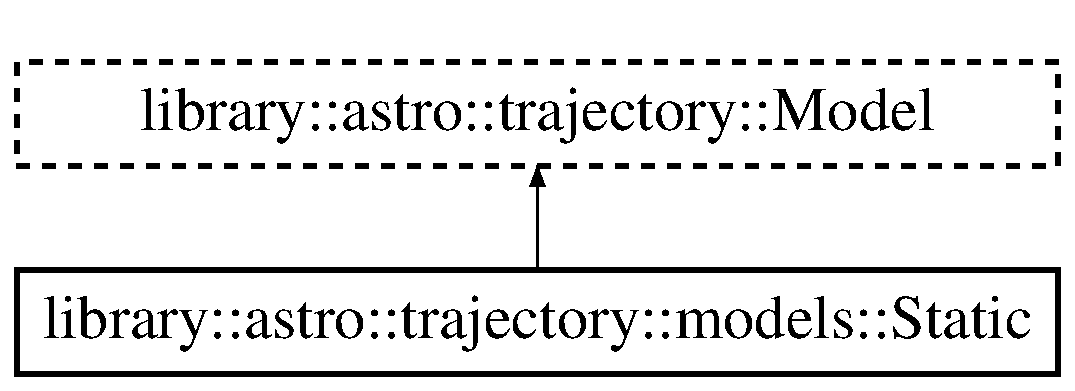
\includegraphics[height=2.000000cm]{classlibrary_1_1astro_1_1trajectory_1_1models_1_1_static}
\end{center}
\end{figure}
\subsection*{Public Member Functions}
\begin{DoxyCompactItemize}
\item 
\hyperlink{classlibrary_1_1astro_1_1trajectory_1_1models_1_1_static_a9d0fc36702a4c78adddc06f8490c83c8}{Static} (const Position \&a\+Position)
\item 
virtual \hyperlink{classlibrary_1_1astro_1_1trajectory_1_1models_1_1_static}{Static} $\ast$ \hyperlink{classlibrary_1_1astro_1_1trajectory_1_1models_1_1_static_a3586bbfdd6fc3958b18a2ffcb3b23fd4}{clone} () const override
\item 
bool \hyperlink{classlibrary_1_1astro_1_1trajectory_1_1models_1_1_static_a9d2238a23ea6666334aece4d3ee04b40}{operator==} (const \hyperlink{classlibrary_1_1astro_1_1trajectory_1_1models_1_1_static}{Static} \&a\+Static\+Model) const
\item 
bool \hyperlink{classlibrary_1_1astro_1_1trajectory_1_1models_1_1_static_a115fe6692bc0946eec93fcf15d382bb4}{operator!=} (const \hyperlink{classlibrary_1_1astro_1_1trajectory_1_1models_1_1_static}{Static} \&a\+Static\+Model) const
\item 
virtual bool \hyperlink{classlibrary_1_1astro_1_1trajectory_1_1models_1_1_static_a41449e98bb076e0601df67b1cfbff6b8}{is\+Defined} () const override
\item 
virtual \hyperlink{classlibrary_1_1astro_1_1trajectory_1_1_state}{State} \hyperlink{classlibrary_1_1astro_1_1trajectory_1_1models_1_1_static_ae4bc6aceab498868e4ebe2a65c6aa413}{calculate\+State\+At} (const Instant \&an\+Instant) const override
\item 
virtual void \hyperlink{classlibrary_1_1astro_1_1trajectory_1_1models_1_1_static_af8f9c6fa6ae2d4471868cc970e1ef571}{print} (std\+::ostream \&an\+Output\+Stream, bool display\+Decorator=true) const override
\end{DoxyCompactItemize}
\subsection*{Protected Member Functions}
\begin{DoxyCompactItemize}
\item 
virtual bool \hyperlink{classlibrary_1_1astro_1_1trajectory_1_1models_1_1_static_ade92be03b036c9625bd5a4111cb69731}{operator==} (const \hyperlink{classlibrary_1_1astro_1_1trajectory_1_1_model}{Model} \&a\+Model) const override
\item 
virtual bool \hyperlink{classlibrary_1_1astro_1_1trajectory_1_1models_1_1_static_aadcfd4ac66cc3fc4cc2b868b9bbc182a}{operator!=} (const \hyperlink{classlibrary_1_1astro_1_1trajectory_1_1_model}{Model} \&a\+Model) const override
\end{DoxyCompactItemize}
\subsection*{Friends}
\begin{DoxyCompactItemize}
\item 
std\+::ostream \& \hyperlink{classlibrary_1_1astro_1_1trajectory_1_1models_1_1_static_a6494cb538d45101dc20cb3910455cb13}{operator$<$$<$} (std\+::ostream \&an\+Output\+Stream, const \hyperlink{classlibrary_1_1astro_1_1trajectory_1_1models_1_1_static}{Static} \&a\+Static\+Model)
\end{DoxyCompactItemize}


\subsection{Detailed Description}
\hyperlink{classlibrary_1_1astro_1_1trajectory_1_1models_1_1_static}{Static} trajectory model. 

\subsection{Constructor \& Destructor Documentation}
\mbox{\Hypertarget{classlibrary_1_1astro_1_1trajectory_1_1models_1_1_static_a9d0fc36702a4c78adddc06f8490c83c8}\label{classlibrary_1_1astro_1_1trajectory_1_1models_1_1_static_a9d0fc36702a4c78adddc06f8490c83c8}} 
\index{library\+::astro\+::trajectory\+::models\+::\+Static@{library\+::astro\+::trajectory\+::models\+::\+Static}!Static@{Static}}
\index{Static@{Static}!library\+::astro\+::trajectory\+::models\+::\+Static@{library\+::astro\+::trajectory\+::models\+::\+Static}}
\subsubsection{\texorpdfstring{Static()}{Static()}}
{\footnotesize\ttfamily library\+::astro\+::trajectory\+::models\+::\+Static\+::\+Static (\begin{DoxyParamCaption}\item[{const Position \&}]{a\+Position }\end{DoxyParamCaption})}



\subsection{Member Function Documentation}
\mbox{\Hypertarget{classlibrary_1_1astro_1_1trajectory_1_1models_1_1_static_ae4bc6aceab498868e4ebe2a65c6aa413}\label{classlibrary_1_1astro_1_1trajectory_1_1models_1_1_static_ae4bc6aceab498868e4ebe2a65c6aa413}} 
\index{library\+::astro\+::trajectory\+::models\+::\+Static@{library\+::astro\+::trajectory\+::models\+::\+Static}!calculate\+State\+At@{calculate\+State\+At}}
\index{calculate\+State\+At@{calculate\+State\+At}!library\+::astro\+::trajectory\+::models\+::\+Static@{library\+::astro\+::trajectory\+::models\+::\+Static}}
\subsubsection{\texorpdfstring{calculate\+State\+At()}{calculateStateAt()}}
{\footnotesize\ttfamily \hyperlink{classlibrary_1_1astro_1_1trajectory_1_1_state}{State} library\+::astro\+::trajectory\+::models\+::\+Static\+::calculate\+State\+At (\begin{DoxyParamCaption}\item[{const Instant \&}]{an\+Instant }\end{DoxyParamCaption}) const\hspace{0.3cm}{\ttfamily [override]}, {\ttfamily [virtual]}}



Implements \hyperlink{classlibrary_1_1astro_1_1trajectory_1_1_model_acee9ee770c2ee1d1205b618e8f722ba4}{library\+::astro\+::trajectory\+::\+Model}.

\mbox{\Hypertarget{classlibrary_1_1astro_1_1trajectory_1_1models_1_1_static_a3586bbfdd6fc3958b18a2ffcb3b23fd4}\label{classlibrary_1_1astro_1_1trajectory_1_1models_1_1_static_a3586bbfdd6fc3958b18a2ffcb3b23fd4}} 
\index{library\+::astro\+::trajectory\+::models\+::\+Static@{library\+::astro\+::trajectory\+::models\+::\+Static}!clone@{clone}}
\index{clone@{clone}!library\+::astro\+::trajectory\+::models\+::\+Static@{library\+::astro\+::trajectory\+::models\+::\+Static}}
\subsubsection{\texorpdfstring{clone()}{clone()}}
{\footnotesize\ttfamily \hyperlink{classlibrary_1_1astro_1_1trajectory_1_1models_1_1_static}{Static} $\ast$ library\+::astro\+::trajectory\+::models\+::\+Static\+::clone (\begin{DoxyParamCaption}{ }\end{DoxyParamCaption}) const\hspace{0.3cm}{\ttfamily [override]}, {\ttfamily [virtual]}}



Implements \hyperlink{classlibrary_1_1astro_1_1trajectory_1_1_model_ad6181e14aea57534897e7446a2a27578}{library\+::astro\+::trajectory\+::\+Model}.

\mbox{\Hypertarget{classlibrary_1_1astro_1_1trajectory_1_1models_1_1_static_a41449e98bb076e0601df67b1cfbff6b8}\label{classlibrary_1_1astro_1_1trajectory_1_1models_1_1_static_a41449e98bb076e0601df67b1cfbff6b8}} 
\index{library\+::astro\+::trajectory\+::models\+::\+Static@{library\+::astro\+::trajectory\+::models\+::\+Static}!is\+Defined@{is\+Defined}}
\index{is\+Defined@{is\+Defined}!library\+::astro\+::trajectory\+::models\+::\+Static@{library\+::astro\+::trajectory\+::models\+::\+Static}}
\subsubsection{\texorpdfstring{is\+Defined()}{isDefined()}}
{\footnotesize\ttfamily bool library\+::astro\+::trajectory\+::models\+::\+Static\+::is\+Defined (\begin{DoxyParamCaption}{ }\end{DoxyParamCaption}) const\hspace{0.3cm}{\ttfamily [override]}, {\ttfamily [virtual]}}



Implements \hyperlink{classlibrary_1_1astro_1_1trajectory_1_1_model_a9b55db62f22c3493313661bacd9f7c1b}{library\+::astro\+::trajectory\+::\+Model}.

\mbox{\Hypertarget{classlibrary_1_1astro_1_1trajectory_1_1models_1_1_static_a115fe6692bc0946eec93fcf15d382bb4}\label{classlibrary_1_1astro_1_1trajectory_1_1models_1_1_static_a115fe6692bc0946eec93fcf15d382bb4}} 
\index{library\+::astro\+::trajectory\+::models\+::\+Static@{library\+::astro\+::trajectory\+::models\+::\+Static}!operator"!=@{operator"!=}}
\index{operator"!=@{operator"!=}!library\+::astro\+::trajectory\+::models\+::\+Static@{library\+::astro\+::trajectory\+::models\+::\+Static}}
\subsubsection{\texorpdfstring{operator"!=()}{operator!=()}\hspace{0.1cm}{\footnotesize\ttfamily [1/2]}}
{\footnotesize\ttfamily bool library\+::astro\+::trajectory\+::models\+::\+Static\+::operator!= (\begin{DoxyParamCaption}\item[{const \hyperlink{classlibrary_1_1astro_1_1trajectory_1_1models_1_1_static}{Static} \&}]{a\+Static\+Model }\end{DoxyParamCaption}) const}

\mbox{\Hypertarget{classlibrary_1_1astro_1_1trajectory_1_1models_1_1_static_aadcfd4ac66cc3fc4cc2b868b9bbc182a}\label{classlibrary_1_1astro_1_1trajectory_1_1models_1_1_static_aadcfd4ac66cc3fc4cc2b868b9bbc182a}} 
\index{library\+::astro\+::trajectory\+::models\+::\+Static@{library\+::astro\+::trajectory\+::models\+::\+Static}!operator"!=@{operator"!=}}
\index{operator"!=@{operator"!=}!library\+::astro\+::trajectory\+::models\+::\+Static@{library\+::astro\+::trajectory\+::models\+::\+Static}}
\subsubsection{\texorpdfstring{operator"!=()}{operator!=()}\hspace{0.1cm}{\footnotesize\ttfamily [2/2]}}
{\footnotesize\ttfamily bool library\+::astro\+::trajectory\+::models\+::\+Static\+::operator!= (\begin{DoxyParamCaption}\item[{const \hyperlink{classlibrary_1_1astro_1_1trajectory_1_1_model}{Model} \&}]{a\+Model }\end{DoxyParamCaption}) const\hspace{0.3cm}{\ttfamily [override]}, {\ttfamily [protected]}, {\ttfamily [virtual]}}



Implements \hyperlink{classlibrary_1_1astro_1_1trajectory_1_1_model_a476c234f5fca1eb75f64f5a96fd83c61}{library\+::astro\+::trajectory\+::\+Model}.

\mbox{\Hypertarget{classlibrary_1_1astro_1_1trajectory_1_1models_1_1_static_a9d2238a23ea6666334aece4d3ee04b40}\label{classlibrary_1_1astro_1_1trajectory_1_1models_1_1_static_a9d2238a23ea6666334aece4d3ee04b40}} 
\index{library\+::astro\+::trajectory\+::models\+::\+Static@{library\+::astro\+::trajectory\+::models\+::\+Static}!operator==@{operator==}}
\index{operator==@{operator==}!library\+::astro\+::trajectory\+::models\+::\+Static@{library\+::astro\+::trajectory\+::models\+::\+Static}}
\subsubsection{\texorpdfstring{operator==()}{operator==()}\hspace{0.1cm}{\footnotesize\ttfamily [1/2]}}
{\footnotesize\ttfamily bool library\+::astro\+::trajectory\+::models\+::\+Static\+::operator== (\begin{DoxyParamCaption}\item[{const \hyperlink{classlibrary_1_1astro_1_1trajectory_1_1models_1_1_static}{Static} \&}]{a\+Static\+Model }\end{DoxyParamCaption}) const}

\mbox{\Hypertarget{classlibrary_1_1astro_1_1trajectory_1_1models_1_1_static_ade92be03b036c9625bd5a4111cb69731}\label{classlibrary_1_1astro_1_1trajectory_1_1models_1_1_static_ade92be03b036c9625bd5a4111cb69731}} 
\index{library\+::astro\+::trajectory\+::models\+::\+Static@{library\+::astro\+::trajectory\+::models\+::\+Static}!operator==@{operator==}}
\index{operator==@{operator==}!library\+::astro\+::trajectory\+::models\+::\+Static@{library\+::astro\+::trajectory\+::models\+::\+Static}}
\subsubsection{\texorpdfstring{operator==()}{operator==()}\hspace{0.1cm}{\footnotesize\ttfamily [2/2]}}
{\footnotesize\ttfamily bool library\+::astro\+::trajectory\+::models\+::\+Static\+::operator== (\begin{DoxyParamCaption}\item[{const \hyperlink{classlibrary_1_1astro_1_1trajectory_1_1_model}{Model} \&}]{a\+Model }\end{DoxyParamCaption}) const\hspace{0.3cm}{\ttfamily [override]}, {\ttfamily [protected]}, {\ttfamily [virtual]}}



Implements \hyperlink{classlibrary_1_1astro_1_1trajectory_1_1_model_a83c52eb23e8feea58d600c87700ed923}{library\+::astro\+::trajectory\+::\+Model}.

\mbox{\Hypertarget{classlibrary_1_1astro_1_1trajectory_1_1models_1_1_static_af8f9c6fa6ae2d4471868cc970e1ef571}\label{classlibrary_1_1astro_1_1trajectory_1_1models_1_1_static_af8f9c6fa6ae2d4471868cc970e1ef571}} 
\index{library\+::astro\+::trajectory\+::models\+::\+Static@{library\+::astro\+::trajectory\+::models\+::\+Static}!print@{print}}
\index{print@{print}!library\+::astro\+::trajectory\+::models\+::\+Static@{library\+::astro\+::trajectory\+::models\+::\+Static}}
\subsubsection{\texorpdfstring{print()}{print()}}
{\footnotesize\ttfamily void library\+::astro\+::trajectory\+::models\+::\+Static\+::print (\begin{DoxyParamCaption}\item[{std\+::ostream \&}]{an\+Output\+Stream,  }\item[{bool}]{display\+Decorator = {\ttfamily true} }\end{DoxyParamCaption}) const\hspace{0.3cm}{\ttfamily [override]}, {\ttfamily [virtual]}}



Implements \hyperlink{classlibrary_1_1astro_1_1trajectory_1_1_model_af3dd0c38fdbac0b64f689fd8c88c3320}{library\+::astro\+::trajectory\+::\+Model}.



\subsection{Friends And Related Function Documentation}
\mbox{\Hypertarget{classlibrary_1_1astro_1_1trajectory_1_1models_1_1_static_a6494cb538d45101dc20cb3910455cb13}\label{classlibrary_1_1astro_1_1trajectory_1_1models_1_1_static_a6494cb538d45101dc20cb3910455cb13}} 
\index{library\+::astro\+::trajectory\+::models\+::\+Static@{library\+::astro\+::trajectory\+::models\+::\+Static}!operator$<$$<$@{operator$<$$<$}}
\index{operator$<$$<$@{operator$<$$<$}!library\+::astro\+::trajectory\+::models\+::\+Static@{library\+::astro\+::trajectory\+::models\+::\+Static}}
\subsubsection{\texorpdfstring{operator$<$$<$}{operator<<}}
{\footnotesize\ttfamily std\+::ostream\& operator$<$$<$ (\begin{DoxyParamCaption}\item[{std\+::ostream \&}]{an\+Output\+Stream,  }\item[{const \hyperlink{classlibrary_1_1astro_1_1trajectory_1_1models_1_1_static}{Static} \&}]{a\+Static\+Model }\end{DoxyParamCaption})\hspace{0.3cm}{\ttfamily [friend]}}



The documentation for this class was generated from the following files\+:\begin{DoxyCompactItemize}
\item 
include/\+Library/\+Astrodynamics/\+Trajectory/\+Models/\hyperlink{_static_8hpp}{Static.\+hpp}\item 
src/\+Library/\+Astrodynamics/\+Trajectory/\+Models/\hyperlink{_static_8cpp}{Static.\+cpp}\end{DoxyCompactItemize}

\hypertarget{classlibrary_1_1astro_1_1trajectory_1_1orbit_1_1models_1_1_tabulated}{}\section{library\+:\+:astro\+:\+:trajectory\+:\+:orbit\+:\+:models\+:\+:Tabulated Class Reference}
\label{classlibrary_1_1astro_1_1trajectory_1_1orbit_1_1models_1_1_tabulated}\index{library\+::astro\+::trajectory\+::orbit\+::models\+::\+Tabulated@{library\+::astro\+::trajectory\+::orbit\+::models\+::\+Tabulated}}


{\ttfamily \#include $<$Tabulated.\+hpp$>$}

Inheritance diagram for library\+:\+:astro\+:\+:trajectory\+:\+:orbit\+:\+:models\+:\+:Tabulated\+:\begin{figure}[H]
\begin{center}
\leavevmode
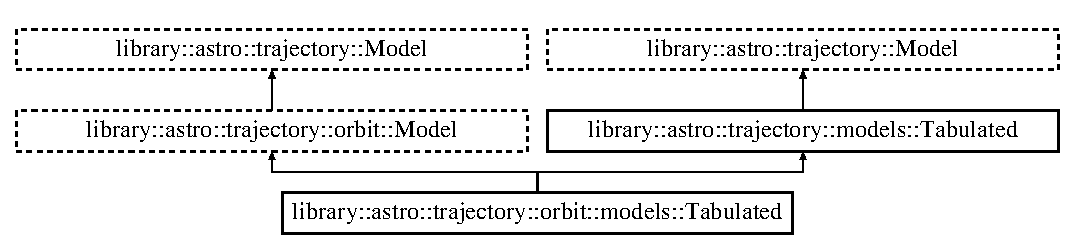
\includegraphics[height=2.916667cm]{classlibrary_1_1astro_1_1trajectory_1_1orbit_1_1models_1_1_tabulated}
\end{center}
\end{figure}
\subsection*{Public Member Functions}
\begin{DoxyCompactItemize}
\item 
\hyperlink{classlibrary_1_1astro_1_1trajectory_1_1orbit_1_1models_1_1_tabulated_a9110680d47c9dcf4272432aa4b299947}{Tabulated} (const Array$<$ \hyperlink{classlibrary_1_1astro_1_1trajectory_1_1_state}{State} $>$ \&a\+State\+Array, const Integer \&an\+Initial\+Revolution\+Number)
\item 
virtual \hyperlink{classlibrary_1_1astro_1_1trajectory_1_1orbit_1_1models_1_1_tabulated}{Tabulated} $\ast$ \hyperlink{classlibrary_1_1astro_1_1trajectory_1_1orbit_1_1models_1_1_tabulated_a8ccec23a49086c6c3fbda2cc81e7a4dc}{clone} () const override
\item 
bool \hyperlink{classlibrary_1_1astro_1_1trajectory_1_1orbit_1_1models_1_1_tabulated_aac67f48eb523ce183d726e6662335969}{operator==} (const \hyperlink{classlibrary_1_1astro_1_1trajectory_1_1orbit_1_1models_1_1_tabulated}{Tabulated} \&a\+Tabulated\+Model) const
\item 
bool \hyperlink{classlibrary_1_1astro_1_1trajectory_1_1orbit_1_1models_1_1_tabulated_a77401f8044dd31fe8ce843091440e27b}{operator!=} (const \hyperlink{classlibrary_1_1astro_1_1trajectory_1_1orbit_1_1models_1_1_tabulated}{Tabulated} \&a\+Tabulated\+Model) const
\item 
virtual bool \hyperlink{classlibrary_1_1astro_1_1trajectory_1_1orbit_1_1models_1_1_tabulated_af68120eb6651e8461c02a465923e533f}{is\+Defined} () const override
\item 
virtual Instant \hyperlink{classlibrary_1_1astro_1_1trajectory_1_1orbit_1_1models_1_1_tabulated_a9e12e7f7b79bf8d2d37494ff7a55ae1d}{get\+Epoch} () const override
\item 
virtual Integer \hyperlink{classlibrary_1_1astro_1_1trajectory_1_1orbit_1_1models_1_1_tabulated_aece7054c261932c3298e8ef2faa2d588}{get\+Revolution\+Number\+At\+Epoch} () const override
\item 
virtual \hyperlink{classlibrary_1_1astro_1_1trajectory_1_1_state}{State} \hyperlink{classlibrary_1_1astro_1_1trajectory_1_1orbit_1_1models_1_1_tabulated_a43db203d7257d25a5a3a6f0e03e62b7d}{calculate\+State\+At} (const Instant \&an\+Instant) const override
\item 
virtual Integer \hyperlink{classlibrary_1_1astro_1_1trajectory_1_1orbit_1_1models_1_1_tabulated_aef0c3d3790f5399c9ae9f78a543a9d5b}{calculate\+Revolution\+Number\+At} (const Instant \&an\+Instant) const override
\item 
virtual void \hyperlink{classlibrary_1_1astro_1_1trajectory_1_1orbit_1_1models_1_1_tabulated_a545a7209580a0c3863f37e2bdd925cb6}{print} (std\+::ostream \&an\+Output\+Stream, bool display\+Decorator) const override
\end{DoxyCompactItemize}
\subsection*{Protected Member Functions}
\begin{DoxyCompactItemize}
\item 
virtual bool \hyperlink{classlibrary_1_1astro_1_1trajectory_1_1orbit_1_1models_1_1_tabulated_a7194a96e062cb6a8c109c82e169a9d7d}{operator==} (const \hyperlink{classlibrary_1_1astro_1_1trajectory_1_1_model}{trajectory\+::\+Model} \&a\+Model) const override
\item 
virtual bool \hyperlink{classlibrary_1_1astro_1_1trajectory_1_1orbit_1_1models_1_1_tabulated_a4373b98c6026c999da98e1740c784e17}{operator!=} (const \hyperlink{classlibrary_1_1astro_1_1trajectory_1_1_model}{trajectory\+::\+Model} \&a\+Model) const override
\end{DoxyCompactItemize}
\subsection*{Additional Inherited Members}


\subsection{Constructor \& Destructor Documentation}
\mbox{\Hypertarget{classlibrary_1_1astro_1_1trajectory_1_1orbit_1_1models_1_1_tabulated_a9110680d47c9dcf4272432aa4b299947}\label{classlibrary_1_1astro_1_1trajectory_1_1orbit_1_1models_1_1_tabulated_a9110680d47c9dcf4272432aa4b299947}} 
\index{library\+::astro\+::trajectory\+::orbit\+::models\+::\+Tabulated@{library\+::astro\+::trajectory\+::orbit\+::models\+::\+Tabulated}!Tabulated@{Tabulated}}
\index{Tabulated@{Tabulated}!library\+::astro\+::trajectory\+::orbit\+::models\+::\+Tabulated@{library\+::astro\+::trajectory\+::orbit\+::models\+::\+Tabulated}}
\subsubsection{\texorpdfstring{Tabulated()}{Tabulated()}}
{\footnotesize\ttfamily library\+::astro\+::trajectory\+::orbit\+::models\+::\+Tabulated\+::\+Tabulated (\begin{DoxyParamCaption}\item[{const Array$<$ \hyperlink{classlibrary_1_1astro_1_1trajectory_1_1_state}{State} $>$ \&}]{a\+State\+Array,  }\item[{const Integer \&}]{an\+Initial\+Revolution\+Number }\end{DoxyParamCaption})}



\subsection{Member Function Documentation}
\mbox{\Hypertarget{classlibrary_1_1astro_1_1trajectory_1_1orbit_1_1models_1_1_tabulated_aef0c3d3790f5399c9ae9f78a543a9d5b}\label{classlibrary_1_1astro_1_1trajectory_1_1orbit_1_1models_1_1_tabulated_aef0c3d3790f5399c9ae9f78a543a9d5b}} 
\index{library\+::astro\+::trajectory\+::orbit\+::models\+::\+Tabulated@{library\+::astro\+::trajectory\+::orbit\+::models\+::\+Tabulated}!calculate\+Revolution\+Number\+At@{calculate\+Revolution\+Number\+At}}
\index{calculate\+Revolution\+Number\+At@{calculate\+Revolution\+Number\+At}!library\+::astro\+::trajectory\+::orbit\+::models\+::\+Tabulated@{library\+::astro\+::trajectory\+::orbit\+::models\+::\+Tabulated}}
\subsubsection{\texorpdfstring{calculate\+Revolution\+Number\+At()}{calculateRevolutionNumberAt()}}
{\footnotesize\ttfamily Integer library\+::astro\+::trajectory\+::orbit\+::models\+::\+Tabulated\+::calculate\+Revolution\+Number\+At (\begin{DoxyParamCaption}\item[{const Instant \&}]{an\+Instant }\end{DoxyParamCaption}) const\hspace{0.3cm}{\ttfamily [override]}, {\ttfamily [virtual]}}



Implements \hyperlink{classlibrary_1_1astro_1_1trajectory_1_1orbit_1_1_model_a6329db5556ed72aa8ad18515aeaefeab}{library\+::astro\+::trajectory\+::orbit\+::\+Model}.

\mbox{\Hypertarget{classlibrary_1_1astro_1_1trajectory_1_1orbit_1_1models_1_1_tabulated_a43db203d7257d25a5a3a6f0e03e62b7d}\label{classlibrary_1_1astro_1_1trajectory_1_1orbit_1_1models_1_1_tabulated_a43db203d7257d25a5a3a6f0e03e62b7d}} 
\index{library\+::astro\+::trajectory\+::orbit\+::models\+::\+Tabulated@{library\+::astro\+::trajectory\+::orbit\+::models\+::\+Tabulated}!calculate\+State\+At@{calculate\+State\+At}}
\index{calculate\+State\+At@{calculate\+State\+At}!library\+::astro\+::trajectory\+::orbit\+::models\+::\+Tabulated@{library\+::astro\+::trajectory\+::orbit\+::models\+::\+Tabulated}}
\subsubsection{\texorpdfstring{calculate\+State\+At()}{calculateStateAt()}}
{\footnotesize\ttfamily \hyperlink{classlibrary_1_1astro_1_1trajectory_1_1_state}{State} library\+::astro\+::trajectory\+::orbit\+::models\+::\+Tabulated\+::calculate\+State\+At (\begin{DoxyParamCaption}\item[{const Instant \&}]{an\+Instant }\end{DoxyParamCaption}) const\hspace{0.3cm}{\ttfamily [override]}, {\ttfamily [virtual]}}



Reimplemented from \hyperlink{classlibrary_1_1astro_1_1trajectory_1_1models_1_1_tabulated_a6d23f5721930d9e885eb3b763ab3390a}{library\+::astro\+::trajectory\+::models\+::\+Tabulated}.

\mbox{\Hypertarget{classlibrary_1_1astro_1_1trajectory_1_1orbit_1_1models_1_1_tabulated_a8ccec23a49086c6c3fbda2cc81e7a4dc}\label{classlibrary_1_1astro_1_1trajectory_1_1orbit_1_1models_1_1_tabulated_a8ccec23a49086c6c3fbda2cc81e7a4dc}} 
\index{library\+::astro\+::trajectory\+::orbit\+::models\+::\+Tabulated@{library\+::astro\+::trajectory\+::orbit\+::models\+::\+Tabulated}!clone@{clone}}
\index{clone@{clone}!library\+::astro\+::trajectory\+::orbit\+::models\+::\+Tabulated@{library\+::astro\+::trajectory\+::orbit\+::models\+::\+Tabulated}}
\subsubsection{\texorpdfstring{clone()}{clone()}}
{\footnotesize\ttfamily \hyperlink{classlibrary_1_1astro_1_1trajectory_1_1orbit_1_1models_1_1_tabulated}{Tabulated} $\ast$ library\+::astro\+::trajectory\+::orbit\+::models\+::\+Tabulated\+::clone (\begin{DoxyParamCaption}{ }\end{DoxyParamCaption}) const\hspace{0.3cm}{\ttfamily [override]}, {\ttfamily [virtual]}}



Reimplemented from \hyperlink{classlibrary_1_1astro_1_1trajectory_1_1models_1_1_tabulated_a192cfb0ceb4a11d02578adc9702cabc1}{library\+::astro\+::trajectory\+::models\+::\+Tabulated}.

\mbox{\Hypertarget{classlibrary_1_1astro_1_1trajectory_1_1orbit_1_1models_1_1_tabulated_a9e12e7f7b79bf8d2d37494ff7a55ae1d}\label{classlibrary_1_1astro_1_1trajectory_1_1orbit_1_1models_1_1_tabulated_a9e12e7f7b79bf8d2d37494ff7a55ae1d}} 
\index{library\+::astro\+::trajectory\+::orbit\+::models\+::\+Tabulated@{library\+::astro\+::trajectory\+::orbit\+::models\+::\+Tabulated}!get\+Epoch@{get\+Epoch}}
\index{get\+Epoch@{get\+Epoch}!library\+::astro\+::trajectory\+::orbit\+::models\+::\+Tabulated@{library\+::astro\+::trajectory\+::orbit\+::models\+::\+Tabulated}}
\subsubsection{\texorpdfstring{get\+Epoch()}{getEpoch()}}
{\footnotesize\ttfamily Instant library\+::astro\+::trajectory\+::orbit\+::models\+::\+Tabulated\+::get\+Epoch (\begin{DoxyParamCaption}{ }\end{DoxyParamCaption}) const\hspace{0.3cm}{\ttfamily [override]}, {\ttfamily [virtual]}}



Implements \hyperlink{classlibrary_1_1astro_1_1trajectory_1_1orbit_1_1_model_acdec7ed6eed001c2ab4ac5442699a316}{library\+::astro\+::trajectory\+::orbit\+::\+Model}.

\mbox{\Hypertarget{classlibrary_1_1astro_1_1trajectory_1_1orbit_1_1models_1_1_tabulated_aece7054c261932c3298e8ef2faa2d588}\label{classlibrary_1_1astro_1_1trajectory_1_1orbit_1_1models_1_1_tabulated_aece7054c261932c3298e8ef2faa2d588}} 
\index{library\+::astro\+::trajectory\+::orbit\+::models\+::\+Tabulated@{library\+::astro\+::trajectory\+::orbit\+::models\+::\+Tabulated}!get\+Revolution\+Number\+At\+Epoch@{get\+Revolution\+Number\+At\+Epoch}}
\index{get\+Revolution\+Number\+At\+Epoch@{get\+Revolution\+Number\+At\+Epoch}!library\+::astro\+::trajectory\+::orbit\+::models\+::\+Tabulated@{library\+::astro\+::trajectory\+::orbit\+::models\+::\+Tabulated}}
\subsubsection{\texorpdfstring{get\+Revolution\+Number\+At\+Epoch()}{getRevolutionNumberAtEpoch()}}
{\footnotesize\ttfamily Integer library\+::astro\+::trajectory\+::orbit\+::models\+::\+Tabulated\+::get\+Revolution\+Number\+At\+Epoch (\begin{DoxyParamCaption}{ }\end{DoxyParamCaption}) const\hspace{0.3cm}{\ttfamily [override]}, {\ttfamily [virtual]}}



Implements \hyperlink{classlibrary_1_1astro_1_1trajectory_1_1orbit_1_1_model_a940f5e266feb90ee8264d4c7a8a883f3}{library\+::astro\+::trajectory\+::orbit\+::\+Model}.

\mbox{\Hypertarget{classlibrary_1_1astro_1_1trajectory_1_1orbit_1_1models_1_1_tabulated_af68120eb6651e8461c02a465923e533f}\label{classlibrary_1_1astro_1_1trajectory_1_1orbit_1_1models_1_1_tabulated_af68120eb6651e8461c02a465923e533f}} 
\index{library\+::astro\+::trajectory\+::orbit\+::models\+::\+Tabulated@{library\+::astro\+::trajectory\+::orbit\+::models\+::\+Tabulated}!is\+Defined@{is\+Defined}}
\index{is\+Defined@{is\+Defined}!library\+::astro\+::trajectory\+::orbit\+::models\+::\+Tabulated@{library\+::astro\+::trajectory\+::orbit\+::models\+::\+Tabulated}}
\subsubsection{\texorpdfstring{is\+Defined()}{isDefined()}}
{\footnotesize\ttfamily bool library\+::astro\+::trajectory\+::orbit\+::models\+::\+Tabulated\+::is\+Defined (\begin{DoxyParamCaption}{ }\end{DoxyParamCaption}) const\hspace{0.3cm}{\ttfamily [override]}, {\ttfamily [virtual]}}



Reimplemented from \hyperlink{classlibrary_1_1astro_1_1trajectory_1_1models_1_1_tabulated_ae967e30f6de74405671f992a5920883f}{library\+::astro\+::trajectory\+::models\+::\+Tabulated}.

\mbox{\Hypertarget{classlibrary_1_1astro_1_1trajectory_1_1orbit_1_1models_1_1_tabulated_a77401f8044dd31fe8ce843091440e27b}\label{classlibrary_1_1astro_1_1trajectory_1_1orbit_1_1models_1_1_tabulated_a77401f8044dd31fe8ce843091440e27b}} 
\index{library\+::astro\+::trajectory\+::orbit\+::models\+::\+Tabulated@{library\+::astro\+::trajectory\+::orbit\+::models\+::\+Tabulated}!operator"!=@{operator"!=}}
\index{operator"!=@{operator"!=}!library\+::astro\+::trajectory\+::orbit\+::models\+::\+Tabulated@{library\+::astro\+::trajectory\+::orbit\+::models\+::\+Tabulated}}
\subsubsection{\texorpdfstring{operator"!=()}{operator!=()}\hspace{0.1cm}{\footnotesize\ttfamily [1/2]}}
{\footnotesize\ttfamily bool library\+::astro\+::trajectory\+::orbit\+::models\+::\+Tabulated\+::operator!= (\begin{DoxyParamCaption}\item[{const \hyperlink{classlibrary_1_1astro_1_1trajectory_1_1orbit_1_1models_1_1_tabulated}{Tabulated} \&}]{a\+Tabulated\+Model }\end{DoxyParamCaption}) const}

\mbox{\Hypertarget{classlibrary_1_1astro_1_1trajectory_1_1orbit_1_1models_1_1_tabulated_a4373b98c6026c999da98e1740c784e17}\label{classlibrary_1_1astro_1_1trajectory_1_1orbit_1_1models_1_1_tabulated_a4373b98c6026c999da98e1740c784e17}} 
\index{library\+::astro\+::trajectory\+::orbit\+::models\+::\+Tabulated@{library\+::astro\+::trajectory\+::orbit\+::models\+::\+Tabulated}!operator"!=@{operator"!=}}
\index{operator"!=@{operator"!=}!library\+::astro\+::trajectory\+::orbit\+::models\+::\+Tabulated@{library\+::astro\+::trajectory\+::orbit\+::models\+::\+Tabulated}}
\subsubsection{\texorpdfstring{operator"!=()}{operator!=()}\hspace{0.1cm}{\footnotesize\ttfamily [2/2]}}
{\footnotesize\ttfamily bool library\+::astro\+::trajectory\+::orbit\+::models\+::\+Tabulated\+::operator!= (\begin{DoxyParamCaption}\item[{const \hyperlink{classlibrary_1_1astro_1_1trajectory_1_1_model}{trajectory\+::\+Model} \&}]{a\+Model }\end{DoxyParamCaption}) const\hspace{0.3cm}{\ttfamily [override]}, {\ttfamily [protected]}, {\ttfamily [virtual]}}



Reimplemented from \hyperlink{classlibrary_1_1astro_1_1trajectory_1_1models_1_1_tabulated_ae6b286af87f28d080b523fb879b74109}{library\+::astro\+::trajectory\+::models\+::\+Tabulated}.

\mbox{\Hypertarget{classlibrary_1_1astro_1_1trajectory_1_1orbit_1_1models_1_1_tabulated_aac67f48eb523ce183d726e6662335969}\label{classlibrary_1_1astro_1_1trajectory_1_1orbit_1_1models_1_1_tabulated_aac67f48eb523ce183d726e6662335969}} 
\index{library\+::astro\+::trajectory\+::orbit\+::models\+::\+Tabulated@{library\+::astro\+::trajectory\+::orbit\+::models\+::\+Tabulated}!operator==@{operator==}}
\index{operator==@{operator==}!library\+::astro\+::trajectory\+::orbit\+::models\+::\+Tabulated@{library\+::astro\+::trajectory\+::orbit\+::models\+::\+Tabulated}}
\subsubsection{\texorpdfstring{operator==()}{operator==()}\hspace{0.1cm}{\footnotesize\ttfamily [1/2]}}
{\footnotesize\ttfamily bool library\+::astro\+::trajectory\+::orbit\+::models\+::\+Tabulated\+::operator== (\begin{DoxyParamCaption}\item[{const \hyperlink{classlibrary_1_1astro_1_1trajectory_1_1orbit_1_1models_1_1_tabulated}{Tabulated} \&}]{a\+Tabulated\+Model }\end{DoxyParamCaption}) const}

\mbox{\Hypertarget{classlibrary_1_1astro_1_1trajectory_1_1orbit_1_1models_1_1_tabulated_a7194a96e062cb6a8c109c82e169a9d7d}\label{classlibrary_1_1astro_1_1trajectory_1_1orbit_1_1models_1_1_tabulated_a7194a96e062cb6a8c109c82e169a9d7d}} 
\index{library\+::astro\+::trajectory\+::orbit\+::models\+::\+Tabulated@{library\+::astro\+::trajectory\+::orbit\+::models\+::\+Tabulated}!operator==@{operator==}}
\index{operator==@{operator==}!library\+::astro\+::trajectory\+::orbit\+::models\+::\+Tabulated@{library\+::astro\+::trajectory\+::orbit\+::models\+::\+Tabulated}}
\subsubsection{\texorpdfstring{operator==()}{operator==()}\hspace{0.1cm}{\footnotesize\ttfamily [2/2]}}
{\footnotesize\ttfamily bool library\+::astro\+::trajectory\+::orbit\+::models\+::\+Tabulated\+::operator== (\begin{DoxyParamCaption}\item[{const \hyperlink{classlibrary_1_1astro_1_1trajectory_1_1_model}{trajectory\+::\+Model} \&}]{a\+Model }\end{DoxyParamCaption}) const\hspace{0.3cm}{\ttfamily [override]}, {\ttfamily [protected]}, {\ttfamily [virtual]}}



Reimplemented from \hyperlink{classlibrary_1_1astro_1_1trajectory_1_1models_1_1_tabulated_af733fafd705bd6a1f204acdbaf2e9646}{library\+::astro\+::trajectory\+::models\+::\+Tabulated}.

\mbox{\Hypertarget{classlibrary_1_1astro_1_1trajectory_1_1orbit_1_1models_1_1_tabulated_a545a7209580a0c3863f37e2bdd925cb6}\label{classlibrary_1_1astro_1_1trajectory_1_1orbit_1_1models_1_1_tabulated_a545a7209580a0c3863f37e2bdd925cb6}} 
\index{library\+::astro\+::trajectory\+::orbit\+::models\+::\+Tabulated@{library\+::astro\+::trajectory\+::orbit\+::models\+::\+Tabulated}!print@{print}}
\index{print@{print}!library\+::astro\+::trajectory\+::orbit\+::models\+::\+Tabulated@{library\+::astro\+::trajectory\+::orbit\+::models\+::\+Tabulated}}
\subsubsection{\texorpdfstring{print()}{print()}}
{\footnotesize\ttfamily void library\+::astro\+::trajectory\+::orbit\+::models\+::\+Tabulated\+::print (\begin{DoxyParamCaption}\item[{std\+::ostream \&}]{an\+Output\+Stream,  }\item[{bool}]{display\+Decorator }\end{DoxyParamCaption}) const\hspace{0.3cm}{\ttfamily [override]}, {\ttfamily [virtual]}}



Reimplemented from \hyperlink{classlibrary_1_1astro_1_1trajectory_1_1models_1_1_tabulated_a3eae12849178fe43d30a620edceddd8e}{library\+::astro\+::trajectory\+::models\+::\+Tabulated}.



The documentation for this class was generated from the following files\+:\begin{DoxyCompactItemize}
\item 
include/\+Library/\+Astrodynamics/\+Trajectory/\+Orbit/\+Models/\hyperlink{_orbit_2_models_2_tabulated_8hpp}{Tabulated.\+hpp}\item 
src/\+Library/\+Astrodynamics/\+Trajectory/\+Orbit/\+Models/\hyperlink{_orbit_2_models_2_tabulated_8cpp}{Tabulated.\+cpp}\end{DoxyCompactItemize}

\hypertarget{classlibrary_1_1astro_1_1trajectory_1_1models_1_1_tabulated}{}\section{library\+:\+:astro\+:\+:trajectory\+:\+:models\+:\+:Tabulated Class Reference}
\label{classlibrary_1_1astro_1_1trajectory_1_1models_1_1_tabulated}\index{library\+::astro\+::trajectory\+::models\+::\+Tabulated@{library\+::astro\+::trajectory\+::models\+::\+Tabulated}}


\hyperlink{classlibrary_1_1astro_1_1trajectory_1_1models_1_1_tabulated}{Tabulated} trajectory model.  




{\ttfamily \#include $<$Tabulated.\+hpp$>$}

Inheritance diagram for library\+:\+:astro\+:\+:trajectory\+:\+:models\+:\+:Tabulated\+:\begin{figure}[H]
\begin{center}
\leavevmode
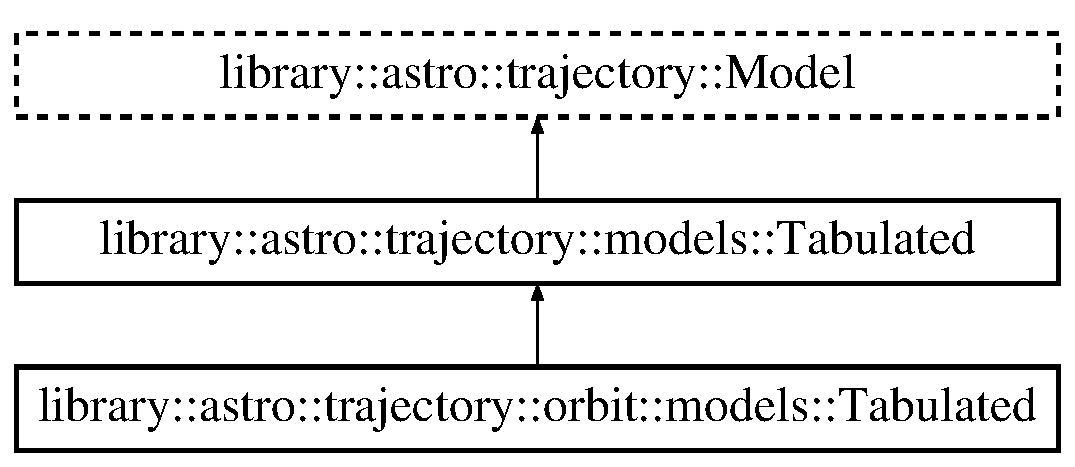
\includegraphics[height=3.000000cm]{classlibrary_1_1astro_1_1trajectory_1_1models_1_1_tabulated}
\end{center}
\end{figure}
\subsection*{Public Member Functions}
\begin{DoxyCompactItemize}
\item 
\hyperlink{classlibrary_1_1astro_1_1trajectory_1_1models_1_1_tabulated_a01461e23723b83bed5dcdd9cac977d14}{Tabulated} (const Array$<$ \hyperlink{classlibrary_1_1astro_1_1trajectory_1_1_state}{State} $>$ \&a\+State\+Array)
\item 
virtual \hyperlink{classlibrary_1_1astro_1_1trajectory_1_1models_1_1_tabulated}{Tabulated} $\ast$ \hyperlink{classlibrary_1_1astro_1_1trajectory_1_1models_1_1_tabulated_a192cfb0ceb4a11d02578adc9702cabc1}{clone} () const override
\item 
bool \hyperlink{classlibrary_1_1astro_1_1trajectory_1_1models_1_1_tabulated_abd07a40a7c4d5dacc8e454d78680b683}{operator==} (const \hyperlink{classlibrary_1_1astro_1_1trajectory_1_1models_1_1_tabulated}{Tabulated} \&a\+Tabulated\+Model) const
\item 
bool \hyperlink{classlibrary_1_1astro_1_1trajectory_1_1models_1_1_tabulated_af6d469ba219acf75e32d64ccebda31f2}{operator!=} (const \hyperlink{classlibrary_1_1astro_1_1trajectory_1_1models_1_1_tabulated}{Tabulated} \&a\+Tabulated\+Model) const
\item 
virtual bool \hyperlink{classlibrary_1_1astro_1_1trajectory_1_1models_1_1_tabulated_ae967e30f6de74405671f992a5920883f}{is\+Defined} () const override
\item 
Interval \hyperlink{classlibrary_1_1astro_1_1trajectory_1_1models_1_1_tabulated_a8c0710d386728b7443469a49c5571e18}{get\+Interval} () const
\item 
virtual \hyperlink{classlibrary_1_1astro_1_1trajectory_1_1_state}{State} \hyperlink{classlibrary_1_1astro_1_1trajectory_1_1models_1_1_tabulated_a6d23f5721930d9e885eb3b763ab3390a}{calculate\+State\+At} (const Instant \&an\+Instant) const override
\item 
virtual void \hyperlink{classlibrary_1_1astro_1_1trajectory_1_1models_1_1_tabulated_a3eae12849178fe43d30a620edceddd8e}{print} (std\+::ostream \&an\+Output\+Stream, bool display\+Decorator=true) const override
\end{DoxyCompactItemize}
\subsection*{Static Public Member Functions}
\begin{DoxyCompactItemize}
\item 
static \hyperlink{classlibrary_1_1astro_1_1trajectory_1_1models_1_1_tabulated}{Tabulated} \hyperlink{classlibrary_1_1astro_1_1trajectory_1_1models_1_1_tabulated_a63c053c7a308930aa03b354292c85c0f}{Load} (const File \&a\+File)
\end{DoxyCompactItemize}
\subsection*{Protected Member Functions}
\begin{DoxyCompactItemize}
\item 
virtual bool \hyperlink{classlibrary_1_1astro_1_1trajectory_1_1models_1_1_tabulated_af733fafd705bd6a1f204acdbaf2e9646}{operator==} (const \hyperlink{classlibrary_1_1astro_1_1trajectory_1_1_model}{Model} \&a\+Model) const override
\item 
virtual bool \hyperlink{classlibrary_1_1astro_1_1trajectory_1_1models_1_1_tabulated_ae6b286af87f28d080b523fb879b74109}{operator!=} (const \hyperlink{classlibrary_1_1astro_1_1trajectory_1_1_model}{Model} \&a\+Model) const override
\end{DoxyCompactItemize}
\subsection*{Friends}
\begin{DoxyCompactItemize}
\item 
std\+::ostream \& \hyperlink{classlibrary_1_1astro_1_1trajectory_1_1models_1_1_tabulated_af2b779226be02822defbe40cf6d3c4b8}{operator$<$$<$} (std\+::ostream \&an\+Output\+Stream, const \hyperlink{classlibrary_1_1astro_1_1trajectory_1_1models_1_1_tabulated}{Tabulated} \&a\+Tabulated\+Model)
\end{DoxyCompactItemize}


\subsection{Detailed Description}
\hyperlink{classlibrary_1_1astro_1_1trajectory_1_1models_1_1_tabulated}{Tabulated} trajectory model. 

For now, a simple linear interpolation is performed between steps. In a future release, more advanced interpolation schemes (quadratic, spline, ...) will be provided. 

\subsection{Constructor \& Destructor Documentation}
\mbox{\Hypertarget{classlibrary_1_1astro_1_1trajectory_1_1models_1_1_tabulated_a01461e23723b83bed5dcdd9cac977d14}\label{classlibrary_1_1astro_1_1trajectory_1_1models_1_1_tabulated_a01461e23723b83bed5dcdd9cac977d14}} 
\index{library\+::astro\+::trajectory\+::models\+::\+Tabulated@{library\+::astro\+::trajectory\+::models\+::\+Tabulated}!Tabulated@{Tabulated}}
\index{Tabulated@{Tabulated}!library\+::astro\+::trajectory\+::models\+::\+Tabulated@{library\+::astro\+::trajectory\+::models\+::\+Tabulated}}
\subsubsection{\texorpdfstring{Tabulated()}{Tabulated()}}
{\footnotesize\ttfamily library\+::astro\+::trajectory\+::models\+::\+Tabulated\+::\+Tabulated (\begin{DoxyParamCaption}\item[{const Array$<$ \hyperlink{classlibrary_1_1astro_1_1trajectory_1_1_state}{State} $>$ \&}]{a\+State\+Array }\end{DoxyParamCaption})}



\subsection{Member Function Documentation}
\mbox{\Hypertarget{classlibrary_1_1astro_1_1trajectory_1_1models_1_1_tabulated_a6d23f5721930d9e885eb3b763ab3390a}\label{classlibrary_1_1astro_1_1trajectory_1_1models_1_1_tabulated_a6d23f5721930d9e885eb3b763ab3390a}} 
\index{library\+::astro\+::trajectory\+::models\+::\+Tabulated@{library\+::astro\+::trajectory\+::models\+::\+Tabulated}!calculate\+State\+At@{calculate\+State\+At}}
\index{calculate\+State\+At@{calculate\+State\+At}!library\+::astro\+::trajectory\+::models\+::\+Tabulated@{library\+::astro\+::trajectory\+::models\+::\+Tabulated}}
\subsubsection{\texorpdfstring{calculate\+State\+At()}{calculateStateAt()}}
{\footnotesize\ttfamily \hyperlink{classlibrary_1_1astro_1_1trajectory_1_1_state}{State} library\+::astro\+::trajectory\+::models\+::\+Tabulated\+::calculate\+State\+At (\begin{DoxyParamCaption}\item[{const Instant \&}]{an\+Instant }\end{DoxyParamCaption}) const\hspace{0.3cm}{\ttfamily [override]}, {\ttfamily [virtual]}}



Implements \hyperlink{classlibrary_1_1astro_1_1trajectory_1_1_model_acee9ee770c2ee1d1205b618e8f722ba4}{library\+::astro\+::trajectory\+::\+Model}.



Reimplemented in \hyperlink{classlibrary_1_1astro_1_1trajectory_1_1orbit_1_1models_1_1_tabulated_a43db203d7257d25a5a3a6f0e03e62b7d}{library\+::astro\+::trajectory\+::orbit\+::models\+::\+Tabulated}.

\mbox{\Hypertarget{classlibrary_1_1astro_1_1trajectory_1_1models_1_1_tabulated_a192cfb0ceb4a11d02578adc9702cabc1}\label{classlibrary_1_1astro_1_1trajectory_1_1models_1_1_tabulated_a192cfb0ceb4a11d02578adc9702cabc1}} 
\index{library\+::astro\+::trajectory\+::models\+::\+Tabulated@{library\+::astro\+::trajectory\+::models\+::\+Tabulated}!clone@{clone}}
\index{clone@{clone}!library\+::astro\+::trajectory\+::models\+::\+Tabulated@{library\+::astro\+::trajectory\+::models\+::\+Tabulated}}
\subsubsection{\texorpdfstring{clone()}{clone()}}
{\footnotesize\ttfamily \hyperlink{classlibrary_1_1astro_1_1trajectory_1_1models_1_1_tabulated}{Tabulated} $\ast$ library\+::astro\+::trajectory\+::models\+::\+Tabulated\+::clone (\begin{DoxyParamCaption}{ }\end{DoxyParamCaption}) const\hspace{0.3cm}{\ttfamily [override]}, {\ttfamily [virtual]}}



Implements \hyperlink{classlibrary_1_1astro_1_1trajectory_1_1_model_ad6181e14aea57534897e7446a2a27578}{library\+::astro\+::trajectory\+::\+Model}.



Reimplemented in \hyperlink{classlibrary_1_1astro_1_1trajectory_1_1orbit_1_1models_1_1_tabulated_a8ccec23a49086c6c3fbda2cc81e7a4dc}{library\+::astro\+::trajectory\+::orbit\+::models\+::\+Tabulated}.

\mbox{\Hypertarget{classlibrary_1_1astro_1_1trajectory_1_1models_1_1_tabulated_a8c0710d386728b7443469a49c5571e18}\label{classlibrary_1_1astro_1_1trajectory_1_1models_1_1_tabulated_a8c0710d386728b7443469a49c5571e18}} 
\index{library\+::astro\+::trajectory\+::models\+::\+Tabulated@{library\+::astro\+::trajectory\+::models\+::\+Tabulated}!get\+Interval@{get\+Interval}}
\index{get\+Interval@{get\+Interval}!library\+::astro\+::trajectory\+::models\+::\+Tabulated@{library\+::astro\+::trajectory\+::models\+::\+Tabulated}}
\subsubsection{\texorpdfstring{get\+Interval()}{getInterval()}}
{\footnotesize\ttfamily Interval library\+::astro\+::trajectory\+::models\+::\+Tabulated\+::get\+Interval (\begin{DoxyParamCaption}{ }\end{DoxyParamCaption}) const}

\mbox{\Hypertarget{classlibrary_1_1astro_1_1trajectory_1_1models_1_1_tabulated_ae967e30f6de74405671f992a5920883f}\label{classlibrary_1_1astro_1_1trajectory_1_1models_1_1_tabulated_ae967e30f6de74405671f992a5920883f}} 
\index{library\+::astro\+::trajectory\+::models\+::\+Tabulated@{library\+::astro\+::trajectory\+::models\+::\+Tabulated}!is\+Defined@{is\+Defined}}
\index{is\+Defined@{is\+Defined}!library\+::astro\+::trajectory\+::models\+::\+Tabulated@{library\+::astro\+::trajectory\+::models\+::\+Tabulated}}
\subsubsection{\texorpdfstring{is\+Defined()}{isDefined()}}
{\footnotesize\ttfamily bool library\+::astro\+::trajectory\+::models\+::\+Tabulated\+::is\+Defined (\begin{DoxyParamCaption}{ }\end{DoxyParamCaption}) const\hspace{0.3cm}{\ttfamily [override]}, {\ttfamily [virtual]}}



Implements \hyperlink{classlibrary_1_1astro_1_1trajectory_1_1_model_a9b55db62f22c3493313661bacd9f7c1b}{library\+::astro\+::trajectory\+::\+Model}.



Reimplemented in \hyperlink{classlibrary_1_1astro_1_1trajectory_1_1orbit_1_1models_1_1_tabulated_af68120eb6651e8461c02a465923e533f}{library\+::astro\+::trajectory\+::orbit\+::models\+::\+Tabulated}.

\mbox{\Hypertarget{classlibrary_1_1astro_1_1trajectory_1_1models_1_1_tabulated_a63c053c7a308930aa03b354292c85c0f}\label{classlibrary_1_1astro_1_1trajectory_1_1models_1_1_tabulated_a63c053c7a308930aa03b354292c85c0f}} 
\index{library\+::astro\+::trajectory\+::models\+::\+Tabulated@{library\+::astro\+::trajectory\+::models\+::\+Tabulated}!Load@{Load}}
\index{Load@{Load}!library\+::astro\+::trajectory\+::models\+::\+Tabulated@{library\+::astro\+::trajectory\+::models\+::\+Tabulated}}
\subsubsection{\texorpdfstring{Load()}{Load()}}
{\footnotesize\ttfamily static \hyperlink{classlibrary_1_1astro_1_1trajectory_1_1models_1_1_tabulated}{Tabulated} library\+::astro\+::trajectory\+::models\+::\+Tabulated\+::\+Load (\begin{DoxyParamCaption}\item[{const File \&}]{a\+File }\end{DoxyParamCaption})\hspace{0.3cm}{\ttfamily [static]}}

\mbox{\Hypertarget{classlibrary_1_1astro_1_1trajectory_1_1models_1_1_tabulated_af6d469ba219acf75e32d64ccebda31f2}\label{classlibrary_1_1astro_1_1trajectory_1_1models_1_1_tabulated_af6d469ba219acf75e32d64ccebda31f2}} 
\index{library\+::astro\+::trajectory\+::models\+::\+Tabulated@{library\+::astro\+::trajectory\+::models\+::\+Tabulated}!operator"!=@{operator"!=}}
\index{operator"!=@{operator"!=}!library\+::astro\+::trajectory\+::models\+::\+Tabulated@{library\+::astro\+::trajectory\+::models\+::\+Tabulated}}
\subsubsection{\texorpdfstring{operator"!=()}{operator!=()}\hspace{0.1cm}{\footnotesize\ttfamily [1/2]}}
{\footnotesize\ttfamily bool library\+::astro\+::trajectory\+::models\+::\+Tabulated\+::operator!= (\begin{DoxyParamCaption}\item[{const \hyperlink{classlibrary_1_1astro_1_1trajectory_1_1models_1_1_tabulated}{Tabulated} \&}]{a\+Tabulated\+Model }\end{DoxyParamCaption}) const}

\mbox{\Hypertarget{classlibrary_1_1astro_1_1trajectory_1_1models_1_1_tabulated_ae6b286af87f28d080b523fb879b74109}\label{classlibrary_1_1astro_1_1trajectory_1_1models_1_1_tabulated_ae6b286af87f28d080b523fb879b74109}} 
\index{library\+::astro\+::trajectory\+::models\+::\+Tabulated@{library\+::astro\+::trajectory\+::models\+::\+Tabulated}!operator"!=@{operator"!=}}
\index{operator"!=@{operator"!=}!library\+::astro\+::trajectory\+::models\+::\+Tabulated@{library\+::astro\+::trajectory\+::models\+::\+Tabulated}}
\subsubsection{\texorpdfstring{operator"!=()}{operator!=()}\hspace{0.1cm}{\footnotesize\ttfamily [2/2]}}
{\footnotesize\ttfamily bool library\+::astro\+::trajectory\+::models\+::\+Tabulated\+::operator!= (\begin{DoxyParamCaption}\item[{const \hyperlink{classlibrary_1_1astro_1_1trajectory_1_1_model}{Model} \&}]{a\+Model }\end{DoxyParamCaption}) const\hspace{0.3cm}{\ttfamily [override]}, {\ttfamily [protected]}, {\ttfamily [virtual]}}



Implements \hyperlink{classlibrary_1_1astro_1_1trajectory_1_1_model_a476c234f5fca1eb75f64f5a96fd83c61}{library\+::astro\+::trajectory\+::\+Model}.



Reimplemented in \hyperlink{classlibrary_1_1astro_1_1trajectory_1_1orbit_1_1models_1_1_tabulated_a4373b98c6026c999da98e1740c784e17}{library\+::astro\+::trajectory\+::orbit\+::models\+::\+Tabulated}.

\mbox{\Hypertarget{classlibrary_1_1astro_1_1trajectory_1_1models_1_1_tabulated_abd07a40a7c4d5dacc8e454d78680b683}\label{classlibrary_1_1astro_1_1trajectory_1_1models_1_1_tabulated_abd07a40a7c4d5dacc8e454d78680b683}} 
\index{library\+::astro\+::trajectory\+::models\+::\+Tabulated@{library\+::astro\+::trajectory\+::models\+::\+Tabulated}!operator==@{operator==}}
\index{operator==@{operator==}!library\+::astro\+::trajectory\+::models\+::\+Tabulated@{library\+::astro\+::trajectory\+::models\+::\+Tabulated}}
\subsubsection{\texorpdfstring{operator==()}{operator==()}\hspace{0.1cm}{\footnotesize\ttfamily [1/2]}}
{\footnotesize\ttfamily bool library\+::astro\+::trajectory\+::models\+::\+Tabulated\+::operator== (\begin{DoxyParamCaption}\item[{const \hyperlink{classlibrary_1_1astro_1_1trajectory_1_1models_1_1_tabulated}{Tabulated} \&}]{a\+Tabulated\+Model }\end{DoxyParamCaption}) const}

\mbox{\Hypertarget{classlibrary_1_1astro_1_1trajectory_1_1models_1_1_tabulated_af733fafd705bd6a1f204acdbaf2e9646}\label{classlibrary_1_1astro_1_1trajectory_1_1models_1_1_tabulated_af733fafd705bd6a1f204acdbaf2e9646}} 
\index{library\+::astro\+::trajectory\+::models\+::\+Tabulated@{library\+::astro\+::trajectory\+::models\+::\+Tabulated}!operator==@{operator==}}
\index{operator==@{operator==}!library\+::astro\+::trajectory\+::models\+::\+Tabulated@{library\+::astro\+::trajectory\+::models\+::\+Tabulated}}
\subsubsection{\texorpdfstring{operator==()}{operator==()}\hspace{0.1cm}{\footnotesize\ttfamily [2/2]}}
{\footnotesize\ttfamily bool library\+::astro\+::trajectory\+::models\+::\+Tabulated\+::operator== (\begin{DoxyParamCaption}\item[{const \hyperlink{classlibrary_1_1astro_1_1trajectory_1_1_model}{Model} \&}]{a\+Model }\end{DoxyParamCaption}) const\hspace{0.3cm}{\ttfamily [override]}, {\ttfamily [protected]}, {\ttfamily [virtual]}}



Implements \hyperlink{classlibrary_1_1astro_1_1trajectory_1_1_model_a83c52eb23e8feea58d600c87700ed923}{library\+::astro\+::trajectory\+::\+Model}.



Reimplemented in \hyperlink{classlibrary_1_1astro_1_1trajectory_1_1orbit_1_1models_1_1_tabulated_a7194a96e062cb6a8c109c82e169a9d7d}{library\+::astro\+::trajectory\+::orbit\+::models\+::\+Tabulated}.

\mbox{\Hypertarget{classlibrary_1_1astro_1_1trajectory_1_1models_1_1_tabulated_a3eae12849178fe43d30a620edceddd8e}\label{classlibrary_1_1astro_1_1trajectory_1_1models_1_1_tabulated_a3eae12849178fe43d30a620edceddd8e}} 
\index{library\+::astro\+::trajectory\+::models\+::\+Tabulated@{library\+::astro\+::trajectory\+::models\+::\+Tabulated}!print@{print}}
\index{print@{print}!library\+::astro\+::trajectory\+::models\+::\+Tabulated@{library\+::astro\+::trajectory\+::models\+::\+Tabulated}}
\subsubsection{\texorpdfstring{print()}{print()}}
{\footnotesize\ttfamily void library\+::astro\+::trajectory\+::models\+::\+Tabulated\+::print (\begin{DoxyParamCaption}\item[{std\+::ostream \&}]{an\+Output\+Stream,  }\item[{bool}]{display\+Decorator = {\ttfamily true} }\end{DoxyParamCaption}) const\hspace{0.3cm}{\ttfamily [override]}, {\ttfamily [virtual]}}



Implements \hyperlink{classlibrary_1_1astro_1_1trajectory_1_1_model_af3dd0c38fdbac0b64f689fd8c88c3320}{library\+::astro\+::trajectory\+::\+Model}.



Reimplemented in \hyperlink{classlibrary_1_1astro_1_1trajectory_1_1orbit_1_1models_1_1_tabulated_a545a7209580a0c3863f37e2bdd925cb6}{library\+::astro\+::trajectory\+::orbit\+::models\+::\+Tabulated}.



\subsection{Friends And Related Function Documentation}
\mbox{\Hypertarget{classlibrary_1_1astro_1_1trajectory_1_1models_1_1_tabulated_af2b779226be02822defbe40cf6d3c4b8}\label{classlibrary_1_1astro_1_1trajectory_1_1models_1_1_tabulated_af2b779226be02822defbe40cf6d3c4b8}} 
\index{library\+::astro\+::trajectory\+::models\+::\+Tabulated@{library\+::astro\+::trajectory\+::models\+::\+Tabulated}!operator$<$$<$@{operator$<$$<$}}
\index{operator$<$$<$@{operator$<$$<$}!library\+::astro\+::trajectory\+::models\+::\+Tabulated@{library\+::astro\+::trajectory\+::models\+::\+Tabulated}}
\subsubsection{\texorpdfstring{operator$<$$<$}{operator<<}}
{\footnotesize\ttfamily std\+::ostream\& operator$<$$<$ (\begin{DoxyParamCaption}\item[{std\+::ostream \&}]{an\+Output\+Stream,  }\item[{const \hyperlink{classlibrary_1_1astro_1_1trajectory_1_1models_1_1_tabulated}{Tabulated} \&}]{a\+Tabulated\+Model }\end{DoxyParamCaption})\hspace{0.3cm}{\ttfamily [friend]}}



The documentation for this class was generated from the following files\+:\begin{DoxyCompactItemize}
\item 
include/\+Library/\+Astrodynamics/\+Trajectory/\+Models/\hyperlink{_models_2_tabulated_8hpp}{Tabulated.\+hpp}\item 
src/\+Library/\+Astrodynamics/\+Trajectory/\+Models/\hyperlink{_models_2_tabulated_8cpp}{Tabulated.\+cpp}\end{DoxyCompactItemize}

\hypertarget{classlibrary_1_1astro_1_1trajectory_1_1orbit_1_1models_1_1sgp4_1_1_t_l_e}{}\section{library\+:\+:astro\+:\+:trajectory\+:\+:orbit\+:\+:models\+:\+:sgp4\+:\+:T\+LE Class Reference}
\label{classlibrary_1_1astro_1_1trajectory_1_1orbit_1_1models_1_1sgp4_1_1_t_l_e}\index{library\+::astro\+::trajectory\+::orbit\+::models\+::sgp4\+::\+T\+LE@{library\+::astro\+::trajectory\+::orbit\+::models\+::sgp4\+::\+T\+LE}}


A Two-\/\+Line Element set (\hyperlink{classlibrary_1_1astro_1_1trajectory_1_1orbit_1_1models_1_1sgp4_1_1_t_l_e}{T\+LE}) is data format encoding a list of orbital elements of an Earth-\/orbiting object for a given point in time.  




{\ttfamily \#include $<$T\+L\+E.\+hpp$>$}

\subsection*{Public Member Functions}
\begin{DoxyCompactItemize}
\item 
\hyperlink{classlibrary_1_1astro_1_1trajectory_1_1orbit_1_1models_1_1sgp4_1_1_t_l_e_a4d2b43f02cef44f0c9635daf9946261c}{T\+LE} (const String \&a\+First\+Line, const String \&a\+Second\+Line)
\begin{DoxyCompactList}\small\item\em Constructor. \end{DoxyCompactList}\item 
\hyperlink{classlibrary_1_1astro_1_1trajectory_1_1orbit_1_1models_1_1sgp4_1_1_t_l_e_ad7e682350d9ed071f254efbfacc1bc07}{T\+LE} (const String \&a\+Satellite\+Name, const String \&a\+First\+Line, const String \&a\+Second\+Line)
\begin{DoxyCompactList}\small\item\em Constructor. \end{DoxyCompactList}\item 
bool \hyperlink{classlibrary_1_1astro_1_1trajectory_1_1orbit_1_1models_1_1sgp4_1_1_t_l_e_aa32fc4cf4703d3137da14da72f7dc684}{operator==} (const \hyperlink{classlibrary_1_1astro_1_1trajectory_1_1orbit_1_1models_1_1sgp4_1_1_t_l_e}{T\+LE} \&a\+Tle) const
\begin{DoxyCompactList}\small\item\em Equal to operator. \end{DoxyCompactList}\item 
bool \hyperlink{classlibrary_1_1astro_1_1trajectory_1_1orbit_1_1models_1_1sgp4_1_1_t_l_e_a92dd1db5b23bbb86f46960c830dcdae3}{operator!=} (const \hyperlink{classlibrary_1_1astro_1_1trajectory_1_1orbit_1_1models_1_1sgp4_1_1_t_l_e}{T\+LE} \&a\+Tle) const
\begin{DoxyCompactList}\small\item\em Not equal to operator. \end{DoxyCompactList}\item 
bool \hyperlink{classlibrary_1_1astro_1_1trajectory_1_1orbit_1_1models_1_1sgp4_1_1_t_l_e_a5098ce1a95f5bcab8398abcf5f3c7101}{is\+Defined} () const
\begin{DoxyCompactList}\small\item\em Check if \hyperlink{classlibrary_1_1astro_1_1trajectory_1_1orbit_1_1models_1_1sgp4_1_1_t_l_e}{T\+LE} is defined. \end{DoxyCompactList}\item 
String \hyperlink{classlibrary_1_1astro_1_1trajectory_1_1orbit_1_1models_1_1sgp4_1_1_t_l_e_a95bb43f9fcf34aee66da615eee909c58}{get\+Satellite\+Name} () const
\begin{DoxyCompactList}\small\item\em Get satellite name. \end{DoxyCompactList}\item 
String \hyperlink{classlibrary_1_1astro_1_1trajectory_1_1orbit_1_1models_1_1sgp4_1_1_t_l_e_a390add219b29b269b22ba2c4d8509fca}{get\+First\+Line} () const
\begin{DoxyCompactList}\small\item\em Get first line. \end{DoxyCompactList}\item 
String \hyperlink{classlibrary_1_1astro_1_1trajectory_1_1orbit_1_1models_1_1sgp4_1_1_t_l_e_a7d4dbf43018504d01585eb1758821aed}{get\+Second\+Line} () const
\begin{DoxyCompactList}\small\item\em Get second line. \end{DoxyCompactList}\item 
Integer \hyperlink{classlibrary_1_1astro_1_1trajectory_1_1orbit_1_1models_1_1sgp4_1_1_t_l_e_acd4260dc4791a44d92e6308a956ff611}{get\+Satellite\+Number} () const
\begin{DoxyCompactList}\small\item\em Get satellite number. \end{DoxyCompactList}\item 
String \hyperlink{classlibrary_1_1astro_1_1trajectory_1_1orbit_1_1models_1_1sgp4_1_1_t_l_e_ae181d950f26600be44624768e31ec3d6}{get\+Classification} () const
\begin{DoxyCompactList}\small\item\em Get classification. \end{DoxyCompactList}\item 
String \hyperlink{classlibrary_1_1astro_1_1trajectory_1_1orbit_1_1models_1_1sgp4_1_1_t_l_e_a20c54ea4314e24dec277ecec17cd2551}{get\+International\+Designator} () const
\begin{DoxyCompactList}\small\item\em Get international designator. \end{DoxyCompactList}\item 
Instant \hyperlink{classlibrary_1_1astro_1_1trajectory_1_1orbit_1_1models_1_1sgp4_1_1_t_l_e_a55543a5f555422eaefab692c19a3d9ea}{get\+Epoch} () const
\begin{DoxyCompactList}\small\item\em Get epoch. \end{DoxyCompactList}\item 
Real \hyperlink{classlibrary_1_1astro_1_1trajectory_1_1orbit_1_1models_1_1sgp4_1_1_t_l_e_ae49c2e82ddcc17462f22f7fa801c81f7}{get\+Mean\+Motion\+First\+Time\+Derivative\+Divided\+By\+Two} () const
\begin{DoxyCompactList}\small\item\em Get first time derivative of the mean motion divided by two. \end{DoxyCompactList}\item 
Real \hyperlink{classlibrary_1_1astro_1_1trajectory_1_1orbit_1_1models_1_1sgp4_1_1_t_l_e_a3363891e156f11b8bbd0cfadb995477d}{get\+Mean\+Motion\+Second\+Time\+Derivative\+Divided\+By\+Six} () const
\begin{DoxyCompactList}\small\item\em Get second time derivative of mean motion divided by six. \end{DoxyCompactList}\item 
Real \hyperlink{classlibrary_1_1astro_1_1trajectory_1_1orbit_1_1models_1_1sgp4_1_1_t_l_e_aaa0c9d0b5027e2fc8a92fb8750bea6a3}{get\+B\+Star\+Drag\+Term} () const
\begin{DoxyCompactList}\small\item\em Get B$\ast$ drag term. \end{DoxyCompactList}\item 
Integer \hyperlink{classlibrary_1_1astro_1_1trajectory_1_1orbit_1_1models_1_1sgp4_1_1_t_l_e_a83621469f7943c96df43cf888d65c60b}{get\+Ephemeris\+Type} () const
\begin{DoxyCompactList}\small\item\em Get ephemeris type (0) \end{DoxyCompactList}\item 
Integer \hyperlink{classlibrary_1_1astro_1_1trajectory_1_1orbit_1_1models_1_1sgp4_1_1_t_l_e_a31ee67f84a2ed0d2353959c0d90ede84}{get\+Element\+Set\+Number} () const
\begin{DoxyCompactList}\small\item\em Get element set number (incremented when a new \hyperlink{classlibrary_1_1astro_1_1trajectory_1_1orbit_1_1models_1_1sgp4_1_1_t_l_e}{T\+LE} is generated for this object) \end{DoxyCompactList}\item 
Integer \hyperlink{classlibrary_1_1astro_1_1trajectory_1_1orbit_1_1models_1_1sgp4_1_1_t_l_e_a6cc7370618c797916a3de07be08c1050}{get\+First\+Line\+Checksum} () const
\begin{DoxyCompactList}\small\item\em Get checksum of first line. \end{DoxyCompactList}\item 
Angle \hyperlink{classlibrary_1_1astro_1_1trajectory_1_1orbit_1_1models_1_1sgp4_1_1_t_l_e_a4443346d4cc2287c2ca55928433c6d60}{get\+Inclination} () const
\begin{DoxyCompactList}\small\item\em Get inclination. \end{DoxyCompactList}\item 
Angle \hyperlink{classlibrary_1_1astro_1_1trajectory_1_1orbit_1_1models_1_1sgp4_1_1_t_l_e_ac6a3af2cbc25d4cc05db3f7a67f16f4b}{get\+Raan} () const
\begin{DoxyCompactList}\small\item\em Get Right Ascension of the Ascending Node \mbox{[}R\+A\+AN\mbox{]}. \end{DoxyCompactList}\item 
Real \hyperlink{classlibrary_1_1astro_1_1trajectory_1_1orbit_1_1models_1_1sgp4_1_1_t_l_e_a26eeb58e67acef61ee83aa3e0932d905}{get\+Eccentricity} () const
\begin{DoxyCompactList}\small\item\em Get eccentricity. \end{DoxyCompactList}\item 
Angle \hyperlink{classlibrary_1_1astro_1_1trajectory_1_1orbit_1_1models_1_1sgp4_1_1_t_l_e_a668a40e4931372f20cf4d533d6f645b1}{get\+Aop} () const
\begin{DoxyCompactList}\small\item\em Get Argument of Perigee \mbox{[}A\+OP\mbox{]}. \end{DoxyCompactList}\item 
Angle \hyperlink{classlibrary_1_1astro_1_1trajectory_1_1orbit_1_1models_1_1sgp4_1_1_t_l_e_a3c63cefb937a2354f7c0051ff90c3fb8}{get\+Mean\+Anomaly} () const
\begin{DoxyCompactList}\small\item\em Get Mean Anomaly. \end{DoxyCompactList}\item 
Derived \hyperlink{classlibrary_1_1astro_1_1trajectory_1_1orbit_1_1models_1_1sgp4_1_1_t_l_e_afe0e7bd5dc0282f1229cbc19feeb8864}{get\+Mean\+Motion} () const
\begin{DoxyCompactList}\small\item\em Get Mean Motion. \end{DoxyCompactList}\item 
Integer \hyperlink{classlibrary_1_1astro_1_1trajectory_1_1orbit_1_1models_1_1sgp4_1_1_t_l_e_ad73649fb07735535b5ba734006a3a628}{get\+Revolution\+Number\+At\+Epoch} () const
\begin{DoxyCompactList}\small\item\em Get revolution number at epoch. \end{DoxyCompactList}\end{DoxyCompactItemize}
\subsection*{Static Public Member Functions}
\begin{DoxyCompactItemize}
\item 
static \hyperlink{classlibrary_1_1astro_1_1trajectory_1_1orbit_1_1models_1_1sgp4_1_1_t_l_e}{T\+LE} \hyperlink{classlibrary_1_1astro_1_1trajectory_1_1orbit_1_1models_1_1sgp4_1_1_t_l_e_ac251783ddaeffea2f48f9cf0bf9aaf5e}{Undefined} ()
\begin{DoxyCompactList}\small\item\em Constructs an undefined \hyperlink{classlibrary_1_1astro_1_1trajectory_1_1orbit_1_1models_1_1sgp4_1_1_t_l_e}{T\+LE}. \end{DoxyCompactList}\item 
static bool \hyperlink{classlibrary_1_1astro_1_1trajectory_1_1orbit_1_1models_1_1sgp4_1_1_t_l_e_a25d768ff21d590d34cd20d4101e07840}{Can\+Parse} (const String \&a\+String)
\begin{DoxyCompactList}\small\item\em Returns true if \hyperlink{classlibrary_1_1astro_1_1trajectory_1_1orbit_1_1models_1_1sgp4_1_1_t_l_e}{T\+LE} can be generated from the given string. \end{DoxyCompactList}\item 
static bool \hyperlink{classlibrary_1_1astro_1_1trajectory_1_1orbit_1_1models_1_1sgp4_1_1_t_l_e_a402cf951360912e70b167bc335c4f9a3}{Can\+Parse} (const String \&a\+First\+Line, const String \&a\+Second\+Line)
\begin{DoxyCompactList}\small\item\em Returns true if \hyperlink{classlibrary_1_1astro_1_1trajectory_1_1orbit_1_1models_1_1sgp4_1_1_t_l_e}{T\+LE} can be generated from the given lines. \end{DoxyCompactList}\item 
static \hyperlink{classlibrary_1_1astro_1_1trajectory_1_1orbit_1_1models_1_1sgp4_1_1_t_l_e}{T\+LE} \hyperlink{classlibrary_1_1astro_1_1trajectory_1_1orbit_1_1models_1_1sgp4_1_1_t_l_e_a842dce63b9adc35c1cb0e21d1777b3a5}{Parse} (const String \&a\+String)
\begin{DoxyCompactList}\small\item\em Constructs a \hyperlink{classlibrary_1_1astro_1_1trajectory_1_1orbit_1_1models_1_1sgp4_1_1_t_l_e}{T\+LE} from a given string. \end{DoxyCompactList}\item 
static \hyperlink{classlibrary_1_1astro_1_1trajectory_1_1orbit_1_1models_1_1sgp4_1_1_t_l_e}{T\+LE} \hyperlink{classlibrary_1_1astro_1_1trajectory_1_1orbit_1_1models_1_1sgp4_1_1_t_l_e_a573d75ef5c2b7ed157dce83fdb556d44}{Load} (const File \&a\+File)
\begin{DoxyCompactList}\small\item\em Load a \hyperlink{classlibrary_1_1astro_1_1trajectory_1_1orbit_1_1models_1_1sgp4_1_1_t_l_e}{T\+LE} from a given file. \end{DoxyCompactList}\end{DoxyCompactItemize}
\subsection*{Friends}
\begin{DoxyCompactItemize}
\item 
std\+::ostream \& \hyperlink{classlibrary_1_1astro_1_1trajectory_1_1orbit_1_1models_1_1sgp4_1_1_t_l_e_a54a7a3bca65674d5052031634f900984}{operator$<$$<$} (std\+::ostream \&an\+Output\+Stream, const \hyperlink{classlibrary_1_1astro_1_1trajectory_1_1orbit_1_1models_1_1sgp4_1_1_t_l_e}{T\+LE} \&a\+Tle)
\begin{DoxyCompactList}\small\item\em Output stream operator. \end{DoxyCompactList}\end{DoxyCompactItemize}


\subsection{Detailed Description}
A Two-\/\+Line Element set (\hyperlink{classlibrary_1_1astro_1_1trajectory_1_1orbit_1_1models_1_1sgp4_1_1_t_l_e}{T\+LE}) is data format encoding a list of orbital elements of an Earth-\/orbiting object for a given point in time. 

https\+://en.wikipedia.\+org/wiki/\+Two-\/line\+\_\+element\+\_\+set 

\subsection{Constructor \& Destructor Documentation}
\mbox{\Hypertarget{classlibrary_1_1astro_1_1trajectory_1_1orbit_1_1models_1_1sgp4_1_1_t_l_e_a4d2b43f02cef44f0c9635daf9946261c}\label{classlibrary_1_1astro_1_1trajectory_1_1orbit_1_1models_1_1sgp4_1_1_t_l_e_a4d2b43f02cef44f0c9635daf9946261c}} 
\index{library\+::astro\+::trajectory\+::orbit\+::models\+::sgp4\+::\+T\+LE@{library\+::astro\+::trajectory\+::orbit\+::models\+::sgp4\+::\+T\+LE}!T\+LE@{T\+LE}}
\index{T\+LE@{T\+LE}!library\+::astro\+::trajectory\+::orbit\+::models\+::sgp4\+::\+T\+LE@{library\+::astro\+::trajectory\+::orbit\+::models\+::sgp4\+::\+T\+LE}}
\subsubsection{\texorpdfstring{T\+L\+E()}{TLE()}\hspace{0.1cm}{\footnotesize\ttfamily [1/2]}}
{\footnotesize\ttfamily library\+::astro\+::trajectory\+::orbit\+::models\+::sgp4\+::\+T\+L\+E\+::\+T\+LE (\begin{DoxyParamCaption}\item[{const String \&}]{a\+First\+Line,  }\item[{const String \&}]{a\+Second\+Line }\end{DoxyParamCaption})}



Constructor. 


\begin{DoxyCode}
\hyperlink{classlibrary_1_1astro_1_1trajectory_1_1orbit_1_1models_1_1sgp4_1_1_t_l_e_a4d2b43f02cef44f0c9635daf9946261c}{TLE} tle(\textcolor{stringliteral}{"1 25544U 98067A   08264.51782528 -.00002182  00000-0 -11606-4 0  2927"},
        \textcolor{stringliteral}{"2 25544  51.6416 247.4627 0006703 130.5360 325.0288 15.72125391563537"}) ;
\end{DoxyCode}



\begin{DoxyParams}[1]{Parameters}
\mbox{\tt in}  & {\em a\+First\+Line} & A first line \\
\hline
\mbox{\tt in}  & {\em a\+Second\+Line} & A second line \\
\hline
\end{DoxyParams}
\mbox{\Hypertarget{classlibrary_1_1astro_1_1trajectory_1_1orbit_1_1models_1_1sgp4_1_1_t_l_e_ad7e682350d9ed071f254efbfacc1bc07}\label{classlibrary_1_1astro_1_1trajectory_1_1orbit_1_1models_1_1sgp4_1_1_t_l_e_ad7e682350d9ed071f254efbfacc1bc07}} 
\index{library\+::astro\+::trajectory\+::orbit\+::models\+::sgp4\+::\+T\+LE@{library\+::astro\+::trajectory\+::orbit\+::models\+::sgp4\+::\+T\+LE}!T\+LE@{T\+LE}}
\index{T\+LE@{T\+LE}!library\+::astro\+::trajectory\+::orbit\+::models\+::sgp4\+::\+T\+LE@{library\+::astro\+::trajectory\+::orbit\+::models\+::sgp4\+::\+T\+LE}}
\subsubsection{\texorpdfstring{T\+L\+E()}{TLE()}\hspace{0.1cm}{\footnotesize\ttfamily [2/2]}}
{\footnotesize\ttfamily library\+::astro\+::trajectory\+::orbit\+::models\+::sgp4\+::\+T\+L\+E\+::\+T\+LE (\begin{DoxyParamCaption}\item[{const String \&}]{a\+Satellite\+Name,  }\item[{const String \&}]{a\+First\+Line,  }\item[{const String \&}]{a\+Second\+Line }\end{DoxyParamCaption})}



Constructor. 


\begin{DoxyCode}
\hyperlink{classlibrary_1_1astro_1_1trajectory_1_1orbit_1_1models_1_1sgp4_1_1_t_l_e_a4d2b43f02cef44f0c9635daf9946261c}{TLE} tle(\textcolor{stringliteral}{"ISS (ZARYA)"},
        \textcolor{stringliteral}{"1 25544U 98067A   08264.51782528 -.00002182  00000-0 -11606-4 0  2927"},
        \textcolor{stringliteral}{"2 25544  51.6416 247.4627 0006703 130.5360 325.0288 15.72125391563537"}) ;
\end{DoxyCode}



\begin{DoxyParams}[1]{Parameters}
\mbox{\tt in}  & {\em a\+Satellite\+Name} & A satellite name \\
\hline
\mbox{\tt in}  & {\em a\+First\+Line} & A first line \\
\hline
\mbox{\tt in}  & {\em a\+Second\+Line} & A second line \\
\hline
\end{DoxyParams}


\subsection{Member Function Documentation}
\mbox{\Hypertarget{classlibrary_1_1astro_1_1trajectory_1_1orbit_1_1models_1_1sgp4_1_1_t_l_e_a25d768ff21d590d34cd20d4101e07840}\label{classlibrary_1_1astro_1_1trajectory_1_1orbit_1_1models_1_1sgp4_1_1_t_l_e_a25d768ff21d590d34cd20d4101e07840}} 
\index{library\+::astro\+::trajectory\+::orbit\+::models\+::sgp4\+::\+T\+LE@{library\+::astro\+::trajectory\+::orbit\+::models\+::sgp4\+::\+T\+LE}!Can\+Parse@{Can\+Parse}}
\index{Can\+Parse@{Can\+Parse}!library\+::astro\+::trajectory\+::orbit\+::models\+::sgp4\+::\+T\+LE@{library\+::astro\+::trajectory\+::orbit\+::models\+::sgp4\+::\+T\+LE}}
\subsubsection{\texorpdfstring{Can\+Parse()}{CanParse()}\hspace{0.1cm}{\footnotesize\ttfamily [1/2]}}
{\footnotesize\ttfamily bool library\+::astro\+::trajectory\+::orbit\+::models\+::sgp4\+::\+T\+L\+E\+::\+Can\+Parse (\begin{DoxyParamCaption}\item[{const String \&}]{a\+String }\end{DoxyParamCaption})\hspace{0.3cm}{\ttfamily [static]}}



Returns true if \hyperlink{classlibrary_1_1astro_1_1trajectory_1_1orbit_1_1models_1_1sgp4_1_1_t_l_e}{T\+LE} can be generated from the given string. 


\begin{DoxyCode}
\hyperlink{classlibrary_1_1astro_1_1trajectory_1_1orbit_1_1models_1_1sgp4_1_1_t_l_e_a25d768ff21d590d34cd20d4101e07840}{TLE::CanParse}(\textcolor{stringliteral}{"1 25544U 98067A   08264.51782528 -.00002182  00000-0 -11606-4 0  2927\(\backslash\)n}
\textcolor{stringliteral}{               2 25544  51.6416 247.4627 0006703 130.5360 325.0288 15.72125391563537"}) ; \textcolor{comment}{// True}
\end{DoxyCode}



\begin{DoxyParams}[1]{Parameters}
\mbox{\tt in}  & {\em a\+String} & A string \\
\hline
\end{DoxyParams}
\begin{DoxyReturn}{Returns}
True if \hyperlink{classlibrary_1_1astro_1_1trajectory_1_1orbit_1_1models_1_1sgp4_1_1_t_l_e}{T\+LE} can be generated from the given string 
\end{DoxyReturn}
\mbox{\Hypertarget{classlibrary_1_1astro_1_1trajectory_1_1orbit_1_1models_1_1sgp4_1_1_t_l_e_a402cf951360912e70b167bc335c4f9a3}\label{classlibrary_1_1astro_1_1trajectory_1_1orbit_1_1models_1_1sgp4_1_1_t_l_e_a402cf951360912e70b167bc335c4f9a3}} 
\index{library\+::astro\+::trajectory\+::orbit\+::models\+::sgp4\+::\+T\+LE@{library\+::astro\+::trajectory\+::orbit\+::models\+::sgp4\+::\+T\+LE}!Can\+Parse@{Can\+Parse}}
\index{Can\+Parse@{Can\+Parse}!library\+::astro\+::trajectory\+::orbit\+::models\+::sgp4\+::\+T\+LE@{library\+::astro\+::trajectory\+::orbit\+::models\+::sgp4\+::\+T\+LE}}
\subsubsection{\texorpdfstring{Can\+Parse()}{CanParse()}\hspace{0.1cm}{\footnotesize\ttfamily [2/2]}}
{\footnotesize\ttfamily bool library\+::astro\+::trajectory\+::orbit\+::models\+::sgp4\+::\+T\+L\+E\+::\+Can\+Parse (\begin{DoxyParamCaption}\item[{const String \&}]{a\+First\+Line,  }\item[{const String \&}]{a\+Second\+Line }\end{DoxyParamCaption})\hspace{0.3cm}{\ttfamily [static]}}



Returns true if \hyperlink{classlibrary_1_1astro_1_1trajectory_1_1orbit_1_1models_1_1sgp4_1_1_t_l_e}{T\+LE} can be generated from the given lines. 


\begin{DoxyCode}
\hyperlink{classlibrary_1_1astro_1_1trajectory_1_1orbit_1_1models_1_1sgp4_1_1_t_l_e_a25d768ff21d590d34cd20d4101e07840}{TLE::CanParse}(\textcolor{stringliteral}{"1 25544U 98067A   08264.51782528 -.00002182  00000-0 -11606-4 0  2927"},
              \textcolor{stringliteral}{"2 25544  51.6416 247.4627 0006703 130.5360 325.0288 15.72125391563537"}) ; \textcolor{comment}{// True}
\end{DoxyCode}



\begin{DoxyParams}[1]{Parameters}
\mbox{\tt in}  & {\em a\+First\+Line} & A first line \\
\hline
\mbox{\tt in}  & {\em a\+Second\+Line} & A second line \\
\hline
\end{DoxyParams}
\begin{DoxyReturn}{Returns}
True if \hyperlink{classlibrary_1_1astro_1_1trajectory_1_1orbit_1_1models_1_1sgp4_1_1_t_l_e}{T\+LE} can be generated from the given lines 
\end{DoxyReturn}
\mbox{\Hypertarget{classlibrary_1_1astro_1_1trajectory_1_1orbit_1_1models_1_1sgp4_1_1_t_l_e_a668a40e4931372f20cf4d533d6f645b1}\label{classlibrary_1_1astro_1_1trajectory_1_1orbit_1_1models_1_1sgp4_1_1_t_l_e_a668a40e4931372f20cf4d533d6f645b1}} 
\index{library\+::astro\+::trajectory\+::orbit\+::models\+::sgp4\+::\+T\+LE@{library\+::astro\+::trajectory\+::orbit\+::models\+::sgp4\+::\+T\+LE}!get\+Aop@{get\+Aop}}
\index{get\+Aop@{get\+Aop}!library\+::astro\+::trajectory\+::orbit\+::models\+::sgp4\+::\+T\+LE@{library\+::astro\+::trajectory\+::orbit\+::models\+::sgp4\+::\+T\+LE}}
\subsubsection{\texorpdfstring{get\+Aop()}{getAop()}}
{\footnotesize\ttfamily Angle library\+::astro\+::trajectory\+::orbit\+::models\+::sgp4\+::\+T\+L\+E\+::get\+Aop (\begin{DoxyParamCaption}{ }\end{DoxyParamCaption}) const}



Get Argument of Perigee \mbox{[}A\+OP\mbox{]}. 

\begin{DoxyReturn}{Returns}
Argument of Perigee 
\end{DoxyReturn}
\mbox{\Hypertarget{classlibrary_1_1astro_1_1trajectory_1_1orbit_1_1models_1_1sgp4_1_1_t_l_e_aaa0c9d0b5027e2fc8a92fb8750bea6a3}\label{classlibrary_1_1astro_1_1trajectory_1_1orbit_1_1models_1_1sgp4_1_1_t_l_e_aaa0c9d0b5027e2fc8a92fb8750bea6a3}} 
\index{library\+::astro\+::trajectory\+::orbit\+::models\+::sgp4\+::\+T\+LE@{library\+::astro\+::trajectory\+::orbit\+::models\+::sgp4\+::\+T\+LE}!get\+B\+Star\+Drag\+Term@{get\+B\+Star\+Drag\+Term}}
\index{get\+B\+Star\+Drag\+Term@{get\+B\+Star\+Drag\+Term}!library\+::astro\+::trajectory\+::orbit\+::models\+::sgp4\+::\+T\+LE@{library\+::astro\+::trajectory\+::orbit\+::models\+::sgp4\+::\+T\+LE}}
\subsubsection{\texorpdfstring{get\+B\+Star\+Drag\+Term()}{getBStarDragTerm()}}
{\footnotesize\ttfamily Real library\+::astro\+::trajectory\+::orbit\+::models\+::sgp4\+::\+T\+L\+E\+::get\+B\+Star\+Drag\+Term (\begin{DoxyParamCaption}{ }\end{DoxyParamCaption}) const}



Get B$\ast$ drag term. 

\begin{DoxyReturn}{Returns}
B$\ast$ drag term https\+://en.wikipedia.\+org/wiki/\+B\+S\+T\+AR 
\end{DoxyReturn}
\mbox{\Hypertarget{classlibrary_1_1astro_1_1trajectory_1_1orbit_1_1models_1_1sgp4_1_1_t_l_e_ae181d950f26600be44624768e31ec3d6}\label{classlibrary_1_1astro_1_1trajectory_1_1orbit_1_1models_1_1sgp4_1_1_t_l_e_ae181d950f26600be44624768e31ec3d6}} 
\index{library\+::astro\+::trajectory\+::orbit\+::models\+::sgp4\+::\+T\+LE@{library\+::astro\+::trajectory\+::orbit\+::models\+::sgp4\+::\+T\+LE}!get\+Classification@{get\+Classification}}
\index{get\+Classification@{get\+Classification}!library\+::astro\+::trajectory\+::orbit\+::models\+::sgp4\+::\+T\+LE@{library\+::astro\+::trajectory\+::orbit\+::models\+::sgp4\+::\+T\+LE}}
\subsubsection{\texorpdfstring{get\+Classification()}{getClassification()}}
{\footnotesize\ttfamily String library\+::astro\+::trajectory\+::orbit\+::models\+::sgp4\+::\+T\+L\+E\+::get\+Classification (\begin{DoxyParamCaption}{ }\end{DoxyParamCaption}) const}



Get classification. 

\begin{DoxyReturn}{Returns}
Classification 
\end{DoxyReturn}
\mbox{\Hypertarget{classlibrary_1_1astro_1_1trajectory_1_1orbit_1_1models_1_1sgp4_1_1_t_l_e_a26eeb58e67acef61ee83aa3e0932d905}\label{classlibrary_1_1astro_1_1trajectory_1_1orbit_1_1models_1_1sgp4_1_1_t_l_e_a26eeb58e67acef61ee83aa3e0932d905}} 
\index{library\+::astro\+::trajectory\+::orbit\+::models\+::sgp4\+::\+T\+LE@{library\+::astro\+::trajectory\+::orbit\+::models\+::sgp4\+::\+T\+LE}!get\+Eccentricity@{get\+Eccentricity}}
\index{get\+Eccentricity@{get\+Eccentricity}!library\+::astro\+::trajectory\+::orbit\+::models\+::sgp4\+::\+T\+LE@{library\+::astro\+::trajectory\+::orbit\+::models\+::sgp4\+::\+T\+LE}}
\subsubsection{\texorpdfstring{get\+Eccentricity()}{getEccentricity()}}
{\footnotesize\ttfamily Real library\+::astro\+::trajectory\+::orbit\+::models\+::sgp4\+::\+T\+L\+E\+::get\+Eccentricity (\begin{DoxyParamCaption}{ }\end{DoxyParamCaption}) const}



Get eccentricity. 

\begin{DoxyReturn}{Returns}
Eccentricity 
\end{DoxyReturn}
\mbox{\Hypertarget{classlibrary_1_1astro_1_1trajectory_1_1orbit_1_1models_1_1sgp4_1_1_t_l_e_a31ee67f84a2ed0d2353959c0d90ede84}\label{classlibrary_1_1astro_1_1trajectory_1_1orbit_1_1models_1_1sgp4_1_1_t_l_e_a31ee67f84a2ed0d2353959c0d90ede84}} 
\index{library\+::astro\+::trajectory\+::orbit\+::models\+::sgp4\+::\+T\+LE@{library\+::astro\+::trajectory\+::orbit\+::models\+::sgp4\+::\+T\+LE}!get\+Element\+Set\+Number@{get\+Element\+Set\+Number}}
\index{get\+Element\+Set\+Number@{get\+Element\+Set\+Number}!library\+::astro\+::trajectory\+::orbit\+::models\+::sgp4\+::\+T\+LE@{library\+::astro\+::trajectory\+::orbit\+::models\+::sgp4\+::\+T\+LE}}
\subsubsection{\texorpdfstring{get\+Element\+Set\+Number()}{getElementSetNumber()}}
{\footnotesize\ttfamily Integer library\+::astro\+::trajectory\+::orbit\+::models\+::sgp4\+::\+T\+L\+E\+::get\+Element\+Set\+Number (\begin{DoxyParamCaption}{ }\end{DoxyParamCaption}) const}



Get element set number (incremented when a new \hyperlink{classlibrary_1_1astro_1_1trajectory_1_1orbit_1_1models_1_1sgp4_1_1_t_l_e}{T\+LE} is generated for this object) 

\begin{DoxyReturn}{Returns}
Element set number 
\end{DoxyReturn}
\mbox{\Hypertarget{classlibrary_1_1astro_1_1trajectory_1_1orbit_1_1models_1_1sgp4_1_1_t_l_e_a83621469f7943c96df43cf888d65c60b}\label{classlibrary_1_1astro_1_1trajectory_1_1orbit_1_1models_1_1sgp4_1_1_t_l_e_a83621469f7943c96df43cf888d65c60b}} 
\index{library\+::astro\+::trajectory\+::orbit\+::models\+::sgp4\+::\+T\+LE@{library\+::astro\+::trajectory\+::orbit\+::models\+::sgp4\+::\+T\+LE}!get\+Ephemeris\+Type@{get\+Ephemeris\+Type}}
\index{get\+Ephemeris\+Type@{get\+Ephemeris\+Type}!library\+::astro\+::trajectory\+::orbit\+::models\+::sgp4\+::\+T\+LE@{library\+::astro\+::trajectory\+::orbit\+::models\+::sgp4\+::\+T\+LE}}
\subsubsection{\texorpdfstring{get\+Ephemeris\+Type()}{getEphemerisType()}}
{\footnotesize\ttfamily Integer library\+::astro\+::trajectory\+::orbit\+::models\+::sgp4\+::\+T\+L\+E\+::get\+Ephemeris\+Type (\begin{DoxyParamCaption}{ }\end{DoxyParamCaption}) const}



Get ephemeris type (0) 

\begin{DoxyReturn}{Returns}
Ephemeris type 
\end{DoxyReturn}
\mbox{\Hypertarget{classlibrary_1_1astro_1_1trajectory_1_1orbit_1_1models_1_1sgp4_1_1_t_l_e_a55543a5f555422eaefab692c19a3d9ea}\label{classlibrary_1_1astro_1_1trajectory_1_1orbit_1_1models_1_1sgp4_1_1_t_l_e_a55543a5f555422eaefab692c19a3d9ea}} 
\index{library\+::astro\+::trajectory\+::orbit\+::models\+::sgp4\+::\+T\+LE@{library\+::astro\+::trajectory\+::orbit\+::models\+::sgp4\+::\+T\+LE}!get\+Epoch@{get\+Epoch}}
\index{get\+Epoch@{get\+Epoch}!library\+::astro\+::trajectory\+::orbit\+::models\+::sgp4\+::\+T\+LE@{library\+::astro\+::trajectory\+::orbit\+::models\+::sgp4\+::\+T\+LE}}
\subsubsection{\texorpdfstring{get\+Epoch()}{getEpoch()}}
{\footnotesize\ttfamily Instant library\+::astro\+::trajectory\+::orbit\+::models\+::sgp4\+::\+T\+L\+E\+::get\+Epoch (\begin{DoxyParamCaption}{ }\end{DoxyParamCaption}) const}



Get epoch. 

\begin{DoxyReturn}{Returns}
Epoch 
\end{DoxyReturn}
\mbox{\Hypertarget{classlibrary_1_1astro_1_1trajectory_1_1orbit_1_1models_1_1sgp4_1_1_t_l_e_a390add219b29b269b22ba2c4d8509fca}\label{classlibrary_1_1astro_1_1trajectory_1_1orbit_1_1models_1_1sgp4_1_1_t_l_e_a390add219b29b269b22ba2c4d8509fca}} 
\index{library\+::astro\+::trajectory\+::orbit\+::models\+::sgp4\+::\+T\+LE@{library\+::astro\+::trajectory\+::orbit\+::models\+::sgp4\+::\+T\+LE}!get\+First\+Line@{get\+First\+Line}}
\index{get\+First\+Line@{get\+First\+Line}!library\+::astro\+::trajectory\+::orbit\+::models\+::sgp4\+::\+T\+LE@{library\+::astro\+::trajectory\+::orbit\+::models\+::sgp4\+::\+T\+LE}}
\subsubsection{\texorpdfstring{get\+First\+Line()}{getFirstLine()}}
{\footnotesize\ttfamily String library\+::astro\+::trajectory\+::orbit\+::models\+::sgp4\+::\+T\+L\+E\+::get\+First\+Line (\begin{DoxyParamCaption}{ }\end{DoxyParamCaption}) const}



Get first line. 


\begin{DoxyCode}
\hyperlink{classlibrary_1_1astro_1_1trajectory_1_1orbit_1_1models_1_1sgp4_1_1_t_l_e_a4d2b43f02cef44f0c9635daf9946261c}{TLE}(\textcolor{stringliteral}{"ISS (ZARYA)"},
    \textcolor{stringliteral}{"1 25544U 98067A   08264.51782528 -.00002182  00000-0 -11606-4 0  2927"},
    \textcolor{stringliteral}{"2 25544  51.6416 247.4627 0006703 130.5360 325.0288 15.72125391563537"}).getSatelliteName() ; \textcolor{comment}{// "1
       25544U 98067A   08264.51782528 -.00002182  00000-0 -11606-4 0  2927"}
\end{DoxyCode}


\begin{DoxyReturn}{Returns}
First line 
\end{DoxyReturn}
\mbox{\Hypertarget{classlibrary_1_1astro_1_1trajectory_1_1orbit_1_1models_1_1sgp4_1_1_t_l_e_a6cc7370618c797916a3de07be08c1050}\label{classlibrary_1_1astro_1_1trajectory_1_1orbit_1_1models_1_1sgp4_1_1_t_l_e_a6cc7370618c797916a3de07be08c1050}} 
\index{library\+::astro\+::trajectory\+::orbit\+::models\+::sgp4\+::\+T\+LE@{library\+::astro\+::trajectory\+::orbit\+::models\+::sgp4\+::\+T\+LE}!get\+First\+Line\+Checksum@{get\+First\+Line\+Checksum}}
\index{get\+First\+Line\+Checksum@{get\+First\+Line\+Checksum}!library\+::astro\+::trajectory\+::orbit\+::models\+::sgp4\+::\+T\+LE@{library\+::astro\+::trajectory\+::orbit\+::models\+::sgp4\+::\+T\+LE}}
\subsubsection{\texorpdfstring{get\+First\+Line\+Checksum()}{getFirstLineChecksum()}}
{\footnotesize\ttfamily Integer library\+::astro\+::trajectory\+::orbit\+::models\+::sgp4\+::\+T\+L\+E\+::get\+First\+Line\+Checksum (\begin{DoxyParamCaption}{ }\end{DoxyParamCaption}) const}



Get checksum of first line. 

\begin{DoxyReturn}{Returns}
Checksum of first line 
\end{DoxyReturn}
\mbox{\Hypertarget{classlibrary_1_1astro_1_1trajectory_1_1orbit_1_1models_1_1sgp4_1_1_t_l_e_a4443346d4cc2287c2ca55928433c6d60}\label{classlibrary_1_1astro_1_1trajectory_1_1orbit_1_1models_1_1sgp4_1_1_t_l_e_a4443346d4cc2287c2ca55928433c6d60}} 
\index{library\+::astro\+::trajectory\+::orbit\+::models\+::sgp4\+::\+T\+LE@{library\+::astro\+::trajectory\+::orbit\+::models\+::sgp4\+::\+T\+LE}!get\+Inclination@{get\+Inclination}}
\index{get\+Inclination@{get\+Inclination}!library\+::astro\+::trajectory\+::orbit\+::models\+::sgp4\+::\+T\+LE@{library\+::astro\+::trajectory\+::orbit\+::models\+::sgp4\+::\+T\+LE}}
\subsubsection{\texorpdfstring{get\+Inclination()}{getInclination()}}
{\footnotesize\ttfamily Angle library\+::astro\+::trajectory\+::orbit\+::models\+::sgp4\+::\+T\+L\+E\+::get\+Inclination (\begin{DoxyParamCaption}{ }\end{DoxyParamCaption}) const}



Get inclination. 

\begin{DoxyReturn}{Returns}
Inclination 
\end{DoxyReturn}
\mbox{\Hypertarget{classlibrary_1_1astro_1_1trajectory_1_1orbit_1_1models_1_1sgp4_1_1_t_l_e_a20c54ea4314e24dec277ecec17cd2551}\label{classlibrary_1_1astro_1_1trajectory_1_1orbit_1_1models_1_1sgp4_1_1_t_l_e_a20c54ea4314e24dec277ecec17cd2551}} 
\index{library\+::astro\+::trajectory\+::orbit\+::models\+::sgp4\+::\+T\+LE@{library\+::astro\+::trajectory\+::orbit\+::models\+::sgp4\+::\+T\+LE}!get\+International\+Designator@{get\+International\+Designator}}
\index{get\+International\+Designator@{get\+International\+Designator}!library\+::astro\+::trajectory\+::orbit\+::models\+::sgp4\+::\+T\+LE@{library\+::astro\+::trajectory\+::orbit\+::models\+::sgp4\+::\+T\+LE}}
\subsubsection{\texorpdfstring{get\+International\+Designator()}{getInternationalDesignator()}}
{\footnotesize\ttfamily String library\+::astro\+::trajectory\+::orbit\+::models\+::sgp4\+::\+T\+L\+E\+::get\+International\+Designator (\begin{DoxyParamCaption}{ }\end{DoxyParamCaption}) const}



Get international designator. 

\begin{DoxyReturn}{Returns}
International designator 
\end{DoxyReturn}
\mbox{\Hypertarget{classlibrary_1_1astro_1_1trajectory_1_1orbit_1_1models_1_1sgp4_1_1_t_l_e_a3c63cefb937a2354f7c0051ff90c3fb8}\label{classlibrary_1_1astro_1_1trajectory_1_1orbit_1_1models_1_1sgp4_1_1_t_l_e_a3c63cefb937a2354f7c0051ff90c3fb8}} 
\index{library\+::astro\+::trajectory\+::orbit\+::models\+::sgp4\+::\+T\+LE@{library\+::astro\+::trajectory\+::orbit\+::models\+::sgp4\+::\+T\+LE}!get\+Mean\+Anomaly@{get\+Mean\+Anomaly}}
\index{get\+Mean\+Anomaly@{get\+Mean\+Anomaly}!library\+::astro\+::trajectory\+::orbit\+::models\+::sgp4\+::\+T\+LE@{library\+::astro\+::trajectory\+::orbit\+::models\+::sgp4\+::\+T\+LE}}
\subsubsection{\texorpdfstring{get\+Mean\+Anomaly()}{getMeanAnomaly()}}
{\footnotesize\ttfamily Angle library\+::astro\+::trajectory\+::orbit\+::models\+::sgp4\+::\+T\+L\+E\+::get\+Mean\+Anomaly (\begin{DoxyParamCaption}{ }\end{DoxyParamCaption}) const}



Get Mean Anomaly. 

\begin{DoxyReturn}{Returns}
Mean Anomaly 
\end{DoxyReturn}
\mbox{\Hypertarget{classlibrary_1_1astro_1_1trajectory_1_1orbit_1_1models_1_1sgp4_1_1_t_l_e_afe0e7bd5dc0282f1229cbc19feeb8864}\label{classlibrary_1_1astro_1_1trajectory_1_1orbit_1_1models_1_1sgp4_1_1_t_l_e_afe0e7bd5dc0282f1229cbc19feeb8864}} 
\index{library\+::astro\+::trajectory\+::orbit\+::models\+::sgp4\+::\+T\+LE@{library\+::astro\+::trajectory\+::orbit\+::models\+::sgp4\+::\+T\+LE}!get\+Mean\+Motion@{get\+Mean\+Motion}}
\index{get\+Mean\+Motion@{get\+Mean\+Motion}!library\+::astro\+::trajectory\+::orbit\+::models\+::sgp4\+::\+T\+LE@{library\+::astro\+::trajectory\+::orbit\+::models\+::sgp4\+::\+T\+LE}}
\subsubsection{\texorpdfstring{get\+Mean\+Motion()}{getMeanMotion()}}
{\footnotesize\ttfamily Derived library\+::astro\+::trajectory\+::orbit\+::models\+::sgp4\+::\+T\+L\+E\+::get\+Mean\+Motion (\begin{DoxyParamCaption}{ }\end{DoxyParamCaption}) const}



Get Mean Motion. 

\begin{DoxyReturn}{Returns}
Mean Motion 
\end{DoxyReturn}
\mbox{\Hypertarget{classlibrary_1_1astro_1_1trajectory_1_1orbit_1_1models_1_1sgp4_1_1_t_l_e_ae49c2e82ddcc17462f22f7fa801c81f7}\label{classlibrary_1_1astro_1_1trajectory_1_1orbit_1_1models_1_1sgp4_1_1_t_l_e_ae49c2e82ddcc17462f22f7fa801c81f7}} 
\index{library\+::astro\+::trajectory\+::orbit\+::models\+::sgp4\+::\+T\+LE@{library\+::astro\+::trajectory\+::orbit\+::models\+::sgp4\+::\+T\+LE}!get\+Mean\+Motion\+First\+Time\+Derivative\+Divided\+By\+Two@{get\+Mean\+Motion\+First\+Time\+Derivative\+Divided\+By\+Two}}
\index{get\+Mean\+Motion\+First\+Time\+Derivative\+Divided\+By\+Two@{get\+Mean\+Motion\+First\+Time\+Derivative\+Divided\+By\+Two}!library\+::astro\+::trajectory\+::orbit\+::models\+::sgp4\+::\+T\+LE@{library\+::astro\+::trajectory\+::orbit\+::models\+::sgp4\+::\+T\+LE}}
\subsubsection{\texorpdfstring{get\+Mean\+Motion\+First\+Time\+Derivative\+Divided\+By\+Two()}{getMeanMotionFirstTimeDerivativeDividedByTwo()}}
{\footnotesize\ttfamily Real library\+::astro\+::trajectory\+::orbit\+::models\+::sgp4\+::\+T\+L\+E\+::get\+Mean\+Motion\+First\+Time\+Derivative\+Divided\+By\+Two (\begin{DoxyParamCaption}{ }\end{DoxyParamCaption}) const}



Get first time derivative of the mean motion divided by two. 

\begin{DoxyReturn}{Returns}
First time derivative of the mean motion divided by two 
\end{DoxyReturn}
\mbox{\Hypertarget{classlibrary_1_1astro_1_1trajectory_1_1orbit_1_1models_1_1sgp4_1_1_t_l_e_a3363891e156f11b8bbd0cfadb995477d}\label{classlibrary_1_1astro_1_1trajectory_1_1orbit_1_1models_1_1sgp4_1_1_t_l_e_a3363891e156f11b8bbd0cfadb995477d}} 
\index{library\+::astro\+::trajectory\+::orbit\+::models\+::sgp4\+::\+T\+LE@{library\+::astro\+::trajectory\+::orbit\+::models\+::sgp4\+::\+T\+LE}!get\+Mean\+Motion\+Second\+Time\+Derivative\+Divided\+By\+Six@{get\+Mean\+Motion\+Second\+Time\+Derivative\+Divided\+By\+Six}}
\index{get\+Mean\+Motion\+Second\+Time\+Derivative\+Divided\+By\+Six@{get\+Mean\+Motion\+Second\+Time\+Derivative\+Divided\+By\+Six}!library\+::astro\+::trajectory\+::orbit\+::models\+::sgp4\+::\+T\+LE@{library\+::astro\+::trajectory\+::orbit\+::models\+::sgp4\+::\+T\+LE}}
\subsubsection{\texorpdfstring{get\+Mean\+Motion\+Second\+Time\+Derivative\+Divided\+By\+Six()}{getMeanMotionSecondTimeDerivativeDividedBySix()}}
{\footnotesize\ttfamily Real library\+::astro\+::trajectory\+::orbit\+::models\+::sgp4\+::\+T\+L\+E\+::get\+Mean\+Motion\+Second\+Time\+Derivative\+Divided\+By\+Six (\begin{DoxyParamCaption}{ }\end{DoxyParamCaption}) const}



Get second time derivative of mean motion divided by six. 

\begin{DoxyReturn}{Returns}
Second time derivative of mean motion divided by six 
\end{DoxyReturn}
\mbox{\Hypertarget{classlibrary_1_1astro_1_1trajectory_1_1orbit_1_1models_1_1sgp4_1_1_t_l_e_ac6a3af2cbc25d4cc05db3f7a67f16f4b}\label{classlibrary_1_1astro_1_1trajectory_1_1orbit_1_1models_1_1sgp4_1_1_t_l_e_ac6a3af2cbc25d4cc05db3f7a67f16f4b}} 
\index{library\+::astro\+::trajectory\+::orbit\+::models\+::sgp4\+::\+T\+LE@{library\+::astro\+::trajectory\+::orbit\+::models\+::sgp4\+::\+T\+LE}!get\+Raan@{get\+Raan}}
\index{get\+Raan@{get\+Raan}!library\+::astro\+::trajectory\+::orbit\+::models\+::sgp4\+::\+T\+LE@{library\+::astro\+::trajectory\+::orbit\+::models\+::sgp4\+::\+T\+LE}}
\subsubsection{\texorpdfstring{get\+Raan()}{getRaan()}}
{\footnotesize\ttfamily Angle library\+::astro\+::trajectory\+::orbit\+::models\+::sgp4\+::\+T\+L\+E\+::get\+Raan (\begin{DoxyParamCaption}{ }\end{DoxyParamCaption}) const}



Get Right Ascension of the Ascending Node \mbox{[}R\+A\+AN\mbox{]}. 

\begin{DoxyReturn}{Returns}
Right Ascension of the Ascending Node 
\end{DoxyReturn}
\mbox{\Hypertarget{classlibrary_1_1astro_1_1trajectory_1_1orbit_1_1models_1_1sgp4_1_1_t_l_e_ad73649fb07735535b5ba734006a3a628}\label{classlibrary_1_1astro_1_1trajectory_1_1orbit_1_1models_1_1sgp4_1_1_t_l_e_ad73649fb07735535b5ba734006a3a628}} 
\index{library\+::astro\+::trajectory\+::orbit\+::models\+::sgp4\+::\+T\+LE@{library\+::astro\+::trajectory\+::orbit\+::models\+::sgp4\+::\+T\+LE}!get\+Revolution\+Number\+At\+Epoch@{get\+Revolution\+Number\+At\+Epoch}}
\index{get\+Revolution\+Number\+At\+Epoch@{get\+Revolution\+Number\+At\+Epoch}!library\+::astro\+::trajectory\+::orbit\+::models\+::sgp4\+::\+T\+LE@{library\+::astro\+::trajectory\+::orbit\+::models\+::sgp4\+::\+T\+LE}}
\subsubsection{\texorpdfstring{get\+Revolution\+Number\+At\+Epoch()}{getRevolutionNumberAtEpoch()}}
{\footnotesize\ttfamily Integer library\+::astro\+::trajectory\+::orbit\+::models\+::sgp4\+::\+T\+L\+E\+::get\+Revolution\+Number\+At\+Epoch (\begin{DoxyParamCaption}{ }\end{DoxyParamCaption}) const}



Get revolution number at epoch. 

\begin{DoxyReturn}{Returns}
Revolution number at epoch 
\end{DoxyReturn}
\mbox{\Hypertarget{classlibrary_1_1astro_1_1trajectory_1_1orbit_1_1models_1_1sgp4_1_1_t_l_e_a95bb43f9fcf34aee66da615eee909c58}\label{classlibrary_1_1astro_1_1trajectory_1_1orbit_1_1models_1_1sgp4_1_1_t_l_e_a95bb43f9fcf34aee66da615eee909c58}} 
\index{library\+::astro\+::trajectory\+::orbit\+::models\+::sgp4\+::\+T\+LE@{library\+::astro\+::trajectory\+::orbit\+::models\+::sgp4\+::\+T\+LE}!get\+Satellite\+Name@{get\+Satellite\+Name}}
\index{get\+Satellite\+Name@{get\+Satellite\+Name}!library\+::astro\+::trajectory\+::orbit\+::models\+::sgp4\+::\+T\+LE@{library\+::astro\+::trajectory\+::orbit\+::models\+::sgp4\+::\+T\+LE}}
\subsubsection{\texorpdfstring{get\+Satellite\+Name()}{getSatelliteName()}}
{\footnotesize\ttfamily String library\+::astro\+::trajectory\+::orbit\+::models\+::sgp4\+::\+T\+L\+E\+::get\+Satellite\+Name (\begin{DoxyParamCaption}{ }\end{DoxyParamCaption}) const}



Get satellite name. 


\begin{DoxyCode}
\hyperlink{classlibrary_1_1astro_1_1trajectory_1_1orbit_1_1models_1_1sgp4_1_1_t_l_e_a4d2b43f02cef44f0c9635daf9946261c}{TLE}(\textcolor{stringliteral}{"ISS (ZARYA)"},
    \textcolor{stringliteral}{"1 25544U 98067A   08264.51782528 -.00002182  00000-0 -11606-4 0  2927"},
    \textcolor{stringliteral}{"2 25544  51.6416 247.4627 0006703 130.5360 325.0288 15.72125391563537"}).getSatelliteName() ; \textcolor{comment}{// "ISS
       (ZARYA)"}
\end{DoxyCode}


\begin{DoxyReturn}{Returns}
Satellite name 
\end{DoxyReturn}
\mbox{\Hypertarget{classlibrary_1_1astro_1_1trajectory_1_1orbit_1_1models_1_1sgp4_1_1_t_l_e_acd4260dc4791a44d92e6308a956ff611}\label{classlibrary_1_1astro_1_1trajectory_1_1orbit_1_1models_1_1sgp4_1_1_t_l_e_acd4260dc4791a44d92e6308a956ff611}} 
\index{library\+::astro\+::trajectory\+::orbit\+::models\+::sgp4\+::\+T\+LE@{library\+::astro\+::trajectory\+::orbit\+::models\+::sgp4\+::\+T\+LE}!get\+Satellite\+Number@{get\+Satellite\+Number}}
\index{get\+Satellite\+Number@{get\+Satellite\+Number}!library\+::astro\+::trajectory\+::orbit\+::models\+::sgp4\+::\+T\+LE@{library\+::astro\+::trajectory\+::orbit\+::models\+::sgp4\+::\+T\+LE}}
\subsubsection{\texorpdfstring{get\+Satellite\+Number()}{getSatelliteNumber()}}
{\footnotesize\ttfamily Integer library\+::astro\+::trajectory\+::orbit\+::models\+::sgp4\+::\+T\+L\+E\+::get\+Satellite\+Number (\begin{DoxyParamCaption}{ }\end{DoxyParamCaption}) const}



Get satellite number. 

\begin{DoxyReturn}{Returns}
Satellite number 
\end{DoxyReturn}
\mbox{\Hypertarget{classlibrary_1_1astro_1_1trajectory_1_1orbit_1_1models_1_1sgp4_1_1_t_l_e_a7d4dbf43018504d01585eb1758821aed}\label{classlibrary_1_1astro_1_1trajectory_1_1orbit_1_1models_1_1sgp4_1_1_t_l_e_a7d4dbf43018504d01585eb1758821aed}} 
\index{library\+::astro\+::trajectory\+::orbit\+::models\+::sgp4\+::\+T\+LE@{library\+::astro\+::trajectory\+::orbit\+::models\+::sgp4\+::\+T\+LE}!get\+Second\+Line@{get\+Second\+Line}}
\index{get\+Second\+Line@{get\+Second\+Line}!library\+::astro\+::trajectory\+::orbit\+::models\+::sgp4\+::\+T\+LE@{library\+::astro\+::trajectory\+::orbit\+::models\+::sgp4\+::\+T\+LE}}
\subsubsection{\texorpdfstring{get\+Second\+Line()}{getSecondLine()}}
{\footnotesize\ttfamily String library\+::astro\+::trajectory\+::orbit\+::models\+::sgp4\+::\+T\+L\+E\+::get\+Second\+Line (\begin{DoxyParamCaption}{ }\end{DoxyParamCaption}) const}



Get second line. 


\begin{DoxyCode}
\hyperlink{classlibrary_1_1astro_1_1trajectory_1_1orbit_1_1models_1_1sgp4_1_1_t_l_e_a4d2b43f02cef44f0c9635daf9946261c}{TLE}(\textcolor{stringliteral}{"ISS (ZARYA)"},
    \textcolor{stringliteral}{"1 25544U 98067A   08264.51782528 -.00002182  00000-0 -11606-4 0  2927"},
    \textcolor{stringliteral}{"2 25544  51.6416 247.4627 0006703 130.5360 325.0288 15.72125391563537"}).getSatelliteName() ; \textcolor{comment}{// "2
       25544  51.6416 247.4627 0006703 130.5360 325.0288 15.72125391563537"}
\end{DoxyCode}


\begin{DoxyReturn}{Returns}
Second line 
\end{DoxyReturn}
\mbox{\Hypertarget{classlibrary_1_1astro_1_1trajectory_1_1orbit_1_1models_1_1sgp4_1_1_t_l_e_a5098ce1a95f5bcab8398abcf5f3c7101}\label{classlibrary_1_1astro_1_1trajectory_1_1orbit_1_1models_1_1sgp4_1_1_t_l_e_a5098ce1a95f5bcab8398abcf5f3c7101}} 
\index{library\+::astro\+::trajectory\+::orbit\+::models\+::sgp4\+::\+T\+LE@{library\+::astro\+::trajectory\+::orbit\+::models\+::sgp4\+::\+T\+LE}!is\+Defined@{is\+Defined}}
\index{is\+Defined@{is\+Defined}!library\+::astro\+::trajectory\+::orbit\+::models\+::sgp4\+::\+T\+LE@{library\+::astro\+::trajectory\+::orbit\+::models\+::sgp4\+::\+T\+LE}}
\subsubsection{\texorpdfstring{is\+Defined()}{isDefined()}}
{\footnotesize\ttfamily bool library\+::astro\+::trajectory\+::orbit\+::models\+::sgp4\+::\+T\+L\+E\+::is\+Defined (\begin{DoxyParamCaption}{ }\end{DoxyParamCaption}) const}



Check if \hyperlink{classlibrary_1_1astro_1_1trajectory_1_1orbit_1_1models_1_1sgp4_1_1_t_l_e}{T\+LE} is defined. 


\begin{DoxyCode}
\hyperlink{classlibrary_1_1astro_1_1trajectory_1_1orbit_1_1models_1_1sgp4_1_1_t_l_e_a4d2b43f02cef44f0c9635daf9946261c}{TLE}(\textcolor{stringliteral}{"1 25544U 98067A   08264.51782528 -.00002182  00000-0 -11606-4 0  2927"},
    \textcolor{stringliteral}{"2 25544  51.6416 247.4627 0006703 130.5360 325.0288 15.72125391563537"}).isDefined() ; \textcolor{comment}{// True}
\end{DoxyCode}


\begin{DoxyReturn}{Returns}
True if \hyperlink{classlibrary_1_1astro_1_1trajectory_1_1orbit_1_1models_1_1sgp4_1_1_t_l_e}{T\+LE} is defined 
\end{DoxyReturn}
\mbox{\Hypertarget{classlibrary_1_1astro_1_1trajectory_1_1orbit_1_1models_1_1sgp4_1_1_t_l_e_a573d75ef5c2b7ed157dce83fdb556d44}\label{classlibrary_1_1astro_1_1trajectory_1_1orbit_1_1models_1_1sgp4_1_1_t_l_e_a573d75ef5c2b7ed157dce83fdb556d44}} 
\index{library\+::astro\+::trajectory\+::orbit\+::models\+::sgp4\+::\+T\+LE@{library\+::astro\+::trajectory\+::orbit\+::models\+::sgp4\+::\+T\+LE}!Load@{Load}}
\index{Load@{Load}!library\+::astro\+::trajectory\+::orbit\+::models\+::sgp4\+::\+T\+LE@{library\+::astro\+::trajectory\+::orbit\+::models\+::sgp4\+::\+T\+LE}}
\subsubsection{\texorpdfstring{Load()}{Load()}}
{\footnotesize\ttfamily \hyperlink{classlibrary_1_1astro_1_1trajectory_1_1orbit_1_1models_1_1sgp4_1_1_t_l_e}{T\+LE} library\+::astro\+::trajectory\+::orbit\+::models\+::sgp4\+::\+T\+L\+E\+::\+Load (\begin{DoxyParamCaption}\item[{const File \&}]{a\+File }\end{DoxyParamCaption})\hspace{0.3cm}{\ttfamily [static]}}



Load a \hyperlink{classlibrary_1_1astro_1_1trajectory_1_1orbit_1_1models_1_1sgp4_1_1_t_l_e}{T\+LE} from a given file. 


\begin{DoxyCode}
\hyperlink{classlibrary_1_1astro_1_1trajectory_1_1orbit_1_1models_1_1sgp4_1_1_t_l_e_a4d2b43f02cef44f0c9635daf9946261c}{TLE} tle = TLE::File(File::Path(Path::String(\textcolor{stringliteral}{"/path/to/file.tle"}))) ;
\end{DoxyCode}



\begin{DoxyParams}[1]{Parameters}
\mbox{\tt in}  & {\em a\+File} & A file \\
\hline
\end{DoxyParams}
\begin{DoxyReturn}{Returns}
\hyperlink{classlibrary_1_1astro_1_1trajectory_1_1orbit_1_1models_1_1sgp4_1_1_t_l_e}{T\+LE} 
\end{DoxyReturn}
\mbox{\Hypertarget{classlibrary_1_1astro_1_1trajectory_1_1orbit_1_1models_1_1sgp4_1_1_t_l_e_a92dd1db5b23bbb86f46960c830dcdae3}\label{classlibrary_1_1astro_1_1trajectory_1_1orbit_1_1models_1_1sgp4_1_1_t_l_e_a92dd1db5b23bbb86f46960c830dcdae3}} 
\index{library\+::astro\+::trajectory\+::orbit\+::models\+::sgp4\+::\+T\+LE@{library\+::astro\+::trajectory\+::orbit\+::models\+::sgp4\+::\+T\+LE}!operator"!=@{operator"!=}}
\index{operator"!=@{operator"!=}!library\+::astro\+::trajectory\+::orbit\+::models\+::sgp4\+::\+T\+LE@{library\+::astro\+::trajectory\+::orbit\+::models\+::sgp4\+::\+T\+LE}}
\subsubsection{\texorpdfstring{operator"!=()}{operator!=()}}
{\footnotesize\ttfamily bool library\+::astro\+::trajectory\+::orbit\+::models\+::sgp4\+::\+T\+L\+E\+::operator!= (\begin{DoxyParamCaption}\item[{const \hyperlink{classlibrary_1_1astro_1_1trajectory_1_1orbit_1_1models_1_1sgp4_1_1_t_l_e}{T\+LE} \&}]{a\+Tle }\end{DoxyParamCaption}) const}



Not equal to operator. 


\begin{DoxyCode}
\hyperlink{classlibrary_1_1astro_1_1trajectory_1_1orbit_1_1models_1_1sgp4_1_1_t_l_e_a4d2b43f02cef44f0c9635daf9946261c}{TLE}(\textcolor{stringliteral}{"..."}, \textcolor{stringliteral}{"..."}) != \hyperlink{classlibrary_1_1astro_1_1trajectory_1_1orbit_1_1models_1_1sgp4_1_1_t_l_e_a4d2b43f02cef44f0c9635daf9946261c}{TLE}(\textcolor{stringliteral}{"..."}, \textcolor{stringliteral}{"..."}) ;
\end{DoxyCode}



\begin{DoxyParams}[1]{Parameters}
\mbox{\tt in}  & {\em a\+Tle} & A \hyperlink{classlibrary_1_1astro_1_1trajectory_1_1orbit_1_1models_1_1sgp4_1_1_t_l_e}{T\+LE} \\
\hline
\end{DoxyParams}
\begin{DoxyReturn}{Returns}
True if T\+L\+Es are not equal 
\end{DoxyReturn}
\mbox{\Hypertarget{classlibrary_1_1astro_1_1trajectory_1_1orbit_1_1models_1_1sgp4_1_1_t_l_e_aa32fc4cf4703d3137da14da72f7dc684}\label{classlibrary_1_1astro_1_1trajectory_1_1orbit_1_1models_1_1sgp4_1_1_t_l_e_aa32fc4cf4703d3137da14da72f7dc684}} 
\index{library\+::astro\+::trajectory\+::orbit\+::models\+::sgp4\+::\+T\+LE@{library\+::astro\+::trajectory\+::orbit\+::models\+::sgp4\+::\+T\+LE}!operator==@{operator==}}
\index{operator==@{operator==}!library\+::astro\+::trajectory\+::orbit\+::models\+::sgp4\+::\+T\+LE@{library\+::astro\+::trajectory\+::orbit\+::models\+::sgp4\+::\+T\+LE}}
\subsubsection{\texorpdfstring{operator==()}{operator==()}}
{\footnotesize\ttfamily bool library\+::astro\+::trajectory\+::orbit\+::models\+::sgp4\+::\+T\+L\+E\+::operator== (\begin{DoxyParamCaption}\item[{const \hyperlink{classlibrary_1_1astro_1_1trajectory_1_1orbit_1_1models_1_1sgp4_1_1_t_l_e}{T\+LE} \&}]{a\+Tle }\end{DoxyParamCaption}) const}



Equal to operator. 


\begin{DoxyCode}
\hyperlink{classlibrary_1_1astro_1_1trajectory_1_1orbit_1_1models_1_1sgp4_1_1_t_l_e_a4d2b43f02cef44f0c9635daf9946261c}{TLE}(\textcolor{stringliteral}{"..."}, \textcolor{stringliteral}{"..."}) == \hyperlink{classlibrary_1_1astro_1_1trajectory_1_1orbit_1_1models_1_1sgp4_1_1_t_l_e_a4d2b43f02cef44f0c9635daf9946261c}{TLE}(\textcolor{stringliteral}{"..."}, \textcolor{stringliteral}{"..."}) ;
\end{DoxyCode}



\begin{DoxyParams}[1]{Parameters}
\mbox{\tt in}  & {\em a\+Tle} & A \hyperlink{classlibrary_1_1astro_1_1trajectory_1_1orbit_1_1models_1_1sgp4_1_1_t_l_e}{T\+LE} \\
\hline
\end{DoxyParams}
\begin{DoxyReturn}{Returns}
True if T\+L\+Es are equal 
\end{DoxyReturn}
\mbox{\Hypertarget{classlibrary_1_1astro_1_1trajectory_1_1orbit_1_1models_1_1sgp4_1_1_t_l_e_a842dce63b9adc35c1cb0e21d1777b3a5}\label{classlibrary_1_1astro_1_1trajectory_1_1orbit_1_1models_1_1sgp4_1_1_t_l_e_a842dce63b9adc35c1cb0e21d1777b3a5}} 
\index{library\+::astro\+::trajectory\+::orbit\+::models\+::sgp4\+::\+T\+LE@{library\+::astro\+::trajectory\+::orbit\+::models\+::sgp4\+::\+T\+LE}!Parse@{Parse}}
\index{Parse@{Parse}!library\+::astro\+::trajectory\+::orbit\+::models\+::sgp4\+::\+T\+LE@{library\+::astro\+::trajectory\+::orbit\+::models\+::sgp4\+::\+T\+LE}}
\subsubsection{\texorpdfstring{Parse()}{Parse()}}
{\footnotesize\ttfamily \hyperlink{classlibrary_1_1astro_1_1trajectory_1_1orbit_1_1models_1_1sgp4_1_1_t_l_e}{T\+LE} library\+::astro\+::trajectory\+::orbit\+::models\+::sgp4\+::\+T\+L\+E\+::\+Parse (\begin{DoxyParamCaption}\item[{const String \&}]{a\+String }\end{DoxyParamCaption})\hspace{0.3cm}{\ttfamily [static]}}



Constructs a \hyperlink{classlibrary_1_1astro_1_1trajectory_1_1orbit_1_1models_1_1sgp4_1_1_t_l_e}{T\+LE} from a given string. 


\begin{DoxyCode}
\hyperlink{classlibrary_1_1astro_1_1trajectory_1_1orbit_1_1models_1_1sgp4_1_1_t_l_e_a4d2b43f02cef44f0c9635daf9946261c}{TLE} tle = \hyperlink{classlibrary_1_1astro_1_1trajectory_1_1orbit_1_1models_1_1sgp4_1_1_t_l_e_a842dce63b9adc35c1cb0e21d1777b3a5}{TLE::Parse}(\textcolor{stringliteral}{"1 25544U 98067A   08264.51782528 -.00002182  00000-0 -11606-4 0  2927\(\backslash\)n}
\textcolor{stringliteral}{                      2 25544  51.6416 247.4627 0006703 130.5360 325.0288 15.72125391563537"}) ;
\end{DoxyCode}



\begin{DoxyParams}[1]{Parameters}
\mbox{\tt in}  & {\em a\+String} & A string \\
\hline
\end{DoxyParams}
\begin{DoxyReturn}{Returns}
\hyperlink{classlibrary_1_1astro_1_1trajectory_1_1orbit_1_1models_1_1sgp4_1_1_t_l_e}{T\+LE} 
\end{DoxyReturn}
\mbox{\Hypertarget{classlibrary_1_1astro_1_1trajectory_1_1orbit_1_1models_1_1sgp4_1_1_t_l_e_ac251783ddaeffea2f48f9cf0bf9aaf5e}\label{classlibrary_1_1astro_1_1trajectory_1_1orbit_1_1models_1_1sgp4_1_1_t_l_e_ac251783ddaeffea2f48f9cf0bf9aaf5e}} 
\index{library\+::astro\+::trajectory\+::orbit\+::models\+::sgp4\+::\+T\+LE@{library\+::astro\+::trajectory\+::orbit\+::models\+::sgp4\+::\+T\+LE}!Undefined@{Undefined}}
\index{Undefined@{Undefined}!library\+::astro\+::trajectory\+::orbit\+::models\+::sgp4\+::\+T\+LE@{library\+::astro\+::trajectory\+::orbit\+::models\+::sgp4\+::\+T\+LE}}
\subsubsection{\texorpdfstring{Undefined()}{Undefined()}}
{\footnotesize\ttfamily \hyperlink{classlibrary_1_1astro_1_1trajectory_1_1orbit_1_1models_1_1sgp4_1_1_t_l_e}{T\+LE} library\+::astro\+::trajectory\+::orbit\+::models\+::sgp4\+::\+T\+L\+E\+::\+Undefined (\begin{DoxyParamCaption}{ }\end{DoxyParamCaption})\hspace{0.3cm}{\ttfamily [static]}}



Constructs an undefined \hyperlink{classlibrary_1_1astro_1_1trajectory_1_1orbit_1_1models_1_1sgp4_1_1_t_l_e}{T\+LE}. 


\begin{DoxyCode}
\hyperlink{classlibrary_1_1astro_1_1trajectory_1_1orbit_1_1models_1_1sgp4_1_1_t_l_e_a4d2b43f02cef44f0c9635daf9946261c}{TLE} tle = \hyperlink{classlibrary_1_1astro_1_1trajectory_1_1orbit_1_1models_1_1sgp4_1_1_t_l_e_ac251783ddaeffea2f48f9cf0bf9aaf5e}{TLE::Undefined}() ; \textcolor{comment}{// Undefined}
\end{DoxyCode}


\begin{DoxyReturn}{Returns}
Undefined \hyperlink{classlibrary_1_1astro_1_1trajectory_1_1orbit_1_1models_1_1sgp4_1_1_t_l_e}{T\+LE} 
\end{DoxyReturn}


\subsection{Friends And Related Function Documentation}
\mbox{\Hypertarget{classlibrary_1_1astro_1_1trajectory_1_1orbit_1_1models_1_1sgp4_1_1_t_l_e_a54a7a3bca65674d5052031634f900984}\label{classlibrary_1_1astro_1_1trajectory_1_1orbit_1_1models_1_1sgp4_1_1_t_l_e_a54a7a3bca65674d5052031634f900984}} 
\index{library\+::astro\+::trajectory\+::orbit\+::models\+::sgp4\+::\+T\+LE@{library\+::astro\+::trajectory\+::orbit\+::models\+::sgp4\+::\+T\+LE}!operator$<$$<$@{operator$<$$<$}}
\index{operator$<$$<$@{operator$<$$<$}!library\+::astro\+::trajectory\+::orbit\+::models\+::sgp4\+::\+T\+LE@{library\+::astro\+::trajectory\+::orbit\+::models\+::sgp4\+::\+T\+LE}}
\subsubsection{\texorpdfstring{operator$<$$<$}{operator<<}}
{\footnotesize\ttfamily std\+::ostream\& operator$<$$<$ (\begin{DoxyParamCaption}\item[{std\+::ostream \&}]{an\+Output\+Stream,  }\item[{const \hyperlink{classlibrary_1_1astro_1_1trajectory_1_1orbit_1_1models_1_1sgp4_1_1_t_l_e}{T\+LE} \&}]{a\+Tle }\end{DoxyParamCaption})\hspace{0.3cm}{\ttfamily [friend]}}



Output stream operator. 


\begin{DoxyCode}
\hyperlink{classlibrary_1_1astro_1_1trajectory_1_1orbit_1_1models_1_1sgp4_1_1_t_l_e_a4d2b43f02cef44f0c9635daf9946261c}{TLE} tle(\textcolor{stringliteral}{"..."}, \textcolor{stringliteral}{"..."}) ;
std::cout << tle ;
\end{DoxyCode}



\begin{DoxyParams}[1]{Parameters}
\mbox{\tt in}  & {\em an\+Output\+Stream} & An output stream \\
\hline
\mbox{\tt in}  & {\em a\+Tle} & A \hyperlink{classlibrary_1_1astro_1_1trajectory_1_1orbit_1_1models_1_1sgp4_1_1_t_l_e}{T\+LE} \\
\hline
\end{DoxyParams}
\begin{DoxyReturn}{Returns}
A reference to output stream 
\end{DoxyReturn}


The documentation for this class was generated from the following files\+:\begin{DoxyCompactItemize}
\item 
include/\+Library/\+Astrodynamics/\+Trajectory/\+Orbit/\+Models/\+S\+G\+P4/\hyperlink{_t_l_e_8hpp}{T\+L\+E.\+hpp}\item 
src/\+Library/\+Astrodynamics/\+Trajectory/\+Orbit/\+Models/\+S\+G\+P4/\hyperlink{_t_l_e_8cpp}{T\+L\+E.\+cpp}\end{DoxyCompactItemize}

\hypertarget{classlibrary_1_1astro_1_1_trajectory}{}\section{library\+:\+:astro\+:\+:Trajectory Class Reference}
\label{classlibrary_1_1astro_1_1_trajectory}\index{library\+::astro\+::\+Trajectory@{library\+::astro\+::\+Trajectory}}


Path followed by an object through space as a function of time.  




{\ttfamily \#include $<$Trajectory.\+hpp$>$}

Inheritance diagram for library\+:\+:astro\+:\+:Trajectory\+:\begin{figure}[H]
\begin{center}
\leavevmode
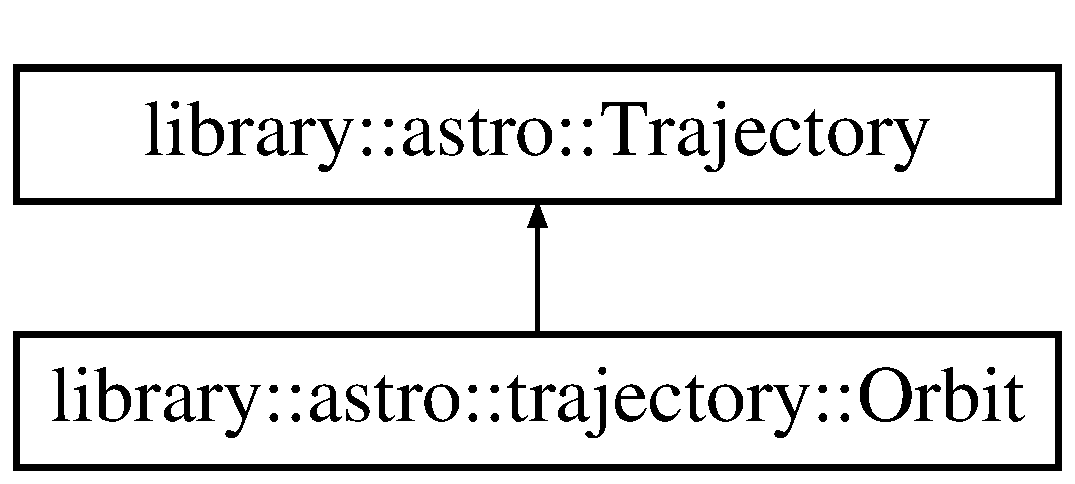
\includegraphics[height=2.000000cm]{classlibrary_1_1astro_1_1_trajectory}
\end{center}
\end{figure}
\subsection*{Public Member Functions}
\begin{DoxyCompactItemize}
\item 
\hyperlink{classlibrary_1_1astro_1_1_trajectory_a8e5c7740915ca947e067c0f419ac1c65}{Trajectory} (const \hyperlink{classlibrary_1_1astro_1_1trajectory_1_1_model}{Model} \&a\+Model)
\begin{DoxyCompactList}\small\item\em Constructor (model) \end{DoxyCompactList}\item 
\hyperlink{classlibrary_1_1astro_1_1_trajectory_abe42247164ca6f966ae5f0c2dfa29182}{Trajectory} (const Array$<$ \hyperlink{classlibrary_1_1astro_1_1trajectory_1_1_state}{State} $>$ \&a\+State\+Array)
\begin{DoxyCompactList}\small\item\em Constructor (state array) \end{DoxyCompactList}\item 
\hyperlink{classlibrary_1_1astro_1_1_trajectory_a63aa2162979ed09fedded192871f0f0a}{Trajectory} (const \hyperlink{classlibrary_1_1astro_1_1_trajectory}{Trajectory} \&a\+Trajectory)
\begin{DoxyCompactList}\small\item\em Copy constructor. \end{DoxyCompactList}\item 
\hyperlink{classlibrary_1_1astro_1_1_trajectory}{Trajectory} \& \hyperlink{classlibrary_1_1astro_1_1_trajectory_abf8200a7b8e08ac9e0f26224fd26cd05}{operator=} (const \hyperlink{classlibrary_1_1astro_1_1_trajectory}{Trajectory} \&a\+Trajectory)=delete
\begin{DoxyCompactList}\small\item\em Copy assignment operator (deleted) \end{DoxyCompactList}\item 
bool \hyperlink{classlibrary_1_1astro_1_1_trajectory_a11bb251602a70c65e727dfc7ed49231e}{operator==} (const \hyperlink{classlibrary_1_1astro_1_1_trajectory}{Trajectory} \&a\+Trajectory) const
\begin{DoxyCompactList}\small\item\em Equal to operator. \end{DoxyCompactList}\item 
bool \hyperlink{classlibrary_1_1astro_1_1_trajectory_a3fa102c5193028fabe84aa7cee9b3e55}{operator!=} (const \hyperlink{classlibrary_1_1astro_1_1_trajectory}{Trajectory} \&a\+Trajectory) const
\begin{DoxyCompactList}\small\item\em Not equal to operator. \end{DoxyCompactList}\item 
bool \hyperlink{classlibrary_1_1astro_1_1_trajectory_aab36edc2566e11d4b5de340cd8230dee}{is\+Defined} () const
\begin{DoxyCompactList}\small\item\em Check if trajectory is defined. \end{DoxyCompactList}\item 
\hyperlink{classlibrary_1_1astro_1_1trajectory_1_1_state}{State} \hyperlink{classlibrary_1_1astro_1_1_trajectory_a5b27c8ad8d547a00ad32c4ab1d63984f}{get\+State\+At} (const Instant \&an\+Instant) const
\begin{DoxyCompactList}\small\item\em Get state at a given instant. \end{DoxyCompactList}\item 
Array$<$ \hyperlink{classlibrary_1_1astro_1_1trajectory_1_1_state}{State} $>$ \hyperlink{classlibrary_1_1astro_1_1_trajectory_a0b7d9ed6012f968b1bfde1f2cc4e34f5}{get\+States\+At} (const Array$<$ Instant $>$ \&an\+Instant\+Array) const
\begin{DoxyCompactList}\small\item\em Get states at a given instants. \end{DoxyCompactList}\item 
virtual void \hyperlink{classlibrary_1_1astro_1_1_trajectory_a6f6afc6bcd8880d7debaa98a79bfa4e6}{print} (std\+::ostream \&an\+Output\+Stream, bool display\+Decorator=true) const
\begin{DoxyCompactList}\small\item\em Print trajectory to output stream. \end{DoxyCompactList}\end{DoxyCompactItemize}
\subsection*{Static Public Member Functions}
\begin{DoxyCompactItemize}
\item 
static \hyperlink{classlibrary_1_1astro_1_1_trajectory}{Trajectory} \hyperlink{classlibrary_1_1astro_1_1_trajectory_a0a8685cabc646fcc5b7f046a606ae967}{Undefined} ()
\begin{DoxyCompactList}\small\item\em Constructs an undefined trajectory. \end{DoxyCompactList}\item 
static \hyperlink{classlibrary_1_1astro_1_1_trajectory}{Trajectory} \hyperlink{classlibrary_1_1astro_1_1_trajectory_a39e9a50f84016cb53ca36d61809dc058}{Position} (const physics\+::coord\+::\+Position \&a\+Position)
\begin{DoxyCompactList}\small\item\em Constructs a trajectory from a given position. \end{DoxyCompactList}\end{DoxyCompactItemize}
\subsection*{Protected Member Functions}
\begin{DoxyCompactItemize}
\item 
const \hyperlink{classlibrary_1_1astro_1_1trajectory_1_1_model}{Model} \& \hyperlink{classlibrary_1_1astro_1_1_trajectory_ac5ebd6f282b52bb3d7c74a79375025e1}{access\+Model} () const
\end{DoxyCompactItemize}
\subsection*{Friends}
\begin{DoxyCompactItemize}
\item 
std\+::ostream \& \hyperlink{classlibrary_1_1astro_1_1_trajectory_aef0327f0240dc2d71eca34dc287f88ea}{operator$<$$<$} (std\+::ostream \&an\+Output\+Stream, const \hyperlink{classlibrary_1_1astro_1_1_trajectory}{Trajectory} \&a\+Trajectory)
\begin{DoxyCompactList}\small\item\em Output stream operator. \end{DoxyCompactList}\end{DoxyCompactItemize}


\subsection{Detailed Description}
Path followed by an object through space as a function of time. 

https\+://en.wikipedia.\+org/wiki/\+Trajectory 

\subsection{Constructor \& Destructor Documentation}
\mbox{\Hypertarget{classlibrary_1_1astro_1_1_trajectory_a8e5c7740915ca947e067c0f419ac1c65}\label{classlibrary_1_1astro_1_1_trajectory_a8e5c7740915ca947e067c0f419ac1c65}} 
\index{library\+::astro\+::\+Trajectory@{library\+::astro\+::\+Trajectory}!Trajectory@{Trajectory}}
\index{Trajectory@{Trajectory}!library\+::astro\+::\+Trajectory@{library\+::astro\+::\+Trajectory}}
\subsubsection{\texorpdfstring{Trajectory()}{Trajectory()}\hspace{0.1cm}{\footnotesize\ttfamily [1/3]}}
{\footnotesize\ttfamily library\+::astro\+::\+Trajectory\+::\+Trajectory (\begin{DoxyParamCaption}\item[{const \hyperlink{classlibrary_1_1astro_1_1trajectory_1_1_model}{Model} \&}]{a\+Model }\end{DoxyParamCaption})}



Constructor (model) 


\begin{DoxyCode}
Tabulated model = \hyperlink{classlibrary_1_1astro_1_1trajectory_1_1models_1_1_tabulated_a63c053c7a308930aa03b354292c85c0f}{Tabulated::Load}(File::Path(Path::Parse(\textcolor{stringliteral}{"/path/to/trajectory.csv"}))) ;
\hyperlink{classlibrary_1_1astro_1_1_trajectory_a8e5c7740915ca947e067c0f419ac1c65}{Trajectory} trajectory = \{ model \} ;
\end{DoxyCode}



\begin{DoxyParams}[1]{Parameters}
\mbox{\tt in}  & {\em a\+Model} & A trajectory model \\
\hline
\end{DoxyParams}
\mbox{\Hypertarget{classlibrary_1_1astro_1_1_trajectory_abe42247164ca6f966ae5f0c2dfa29182}\label{classlibrary_1_1astro_1_1_trajectory_abe42247164ca6f966ae5f0c2dfa29182}} 
\index{library\+::astro\+::\+Trajectory@{library\+::astro\+::\+Trajectory}!Trajectory@{Trajectory}}
\index{Trajectory@{Trajectory}!library\+::astro\+::\+Trajectory@{library\+::astro\+::\+Trajectory}}
\subsubsection{\texorpdfstring{Trajectory()}{Trajectory()}\hspace{0.1cm}{\footnotesize\ttfamily [2/3]}}
{\footnotesize\ttfamily library\+::astro\+::\+Trajectory\+::\+Trajectory (\begin{DoxyParamCaption}\item[{const Array$<$ \hyperlink{classlibrary_1_1astro_1_1trajectory_1_1_state}{State} $>$ \&}]{a\+State\+Array }\end{DoxyParamCaption})}



Constructor (state array) 


\begin{DoxyCode}
Array<State> stateArray = \{ ... \} ;
\hyperlink{classlibrary_1_1astro_1_1_trajectory_a8e5c7740915ca947e067c0f419ac1c65}{Trajectory} trajectory = \{ stateArray \} ;
\end{DoxyCode}



\begin{DoxyParams}[1]{Parameters}
\mbox{\tt in}  & {\em a\+State\+Array} & An array of states \\
\hline
\end{DoxyParams}
\mbox{\Hypertarget{classlibrary_1_1astro_1_1_trajectory_a63aa2162979ed09fedded192871f0f0a}\label{classlibrary_1_1astro_1_1_trajectory_a63aa2162979ed09fedded192871f0f0a}} 
\index{library\+::astro\+::\+Trajectory@{library\+::astro\+::\+Trajectory}!Trajectory@{Trajectory}}
\index{Trajectory@{Trajectory}!library\+::astro\+::\+Trajectory@{library\+::astro\+::\+Trajectory}}
\subsubsection{\texorpdfstring{Trajectory()}{Trajectory()}\hspace{0.1cm}{\footnotesize\ttfamily [3/3]}}
{\footnotesize\ttfamily library\+::astro\+::\+Trajectory\+::\+Trajectory (\begin{DoxyParamCaption}\item[{const \hyperlink{classlibrary_1_1astro_1_1_trajectory}{Trajectory} \&}]{a\+Trajectory }\end{DoxyParamCaption})}



Copy constructor. 


\begin{DoxyParams}[1]{Parameters}
\mbox{\tt in}  & {\em a\+Trajectory} & A trajectory \\
\hline
\end{DoxyParams}


\subsection{Member Function Documentation}
\mbox{\Hypertarget{classlibrary_1_1astro_1_1_trajectory_ac5ebd6f282b52bb3d7c74a79375025e1}\label{classlibrary_1_1astro_1_1_trajectory_ac5ebd6f282b52bb3d7c74a79375025e1}} 
\index{library\+::astro\+::\+Trajectory@{library\+::astro\+::\+Trajectory}!access\+Model@{access\+Model}}
\index{access\+Model@{access\+Model}!library\+::astro\+::\+Trajectory@{library\+::astro\+::\+Trajectory}}
\subsubsection{\texorpdfstring{access\+Model()}{accessModel()}}
{\footnotesize\ttfamily const \hyperlink{classlibrary_1_1astro_1_1trajectory_1_1_model}{Model} \& library\+::astro\+::\+Trajectory\+::access\+Model (\begin{DoxyParamCaption}{ }\end{DoxyParamCaption}) const\hspace{0.3cm}{\ttfamily [protected]}}

\mbox{\Hypertarget{classlibrary_1_1astro_1_1_trajectory_a5b27c8ad8d547a00ad32c4ab1d63984f}\label{classlibrary_1_1astro_1_1_trajectory_a5b27c8ad8d547a00ad32c4ab1d63984f}} 
\index{library\+::astro\+::\+Trajectory@{library\+::astro\+::\+Trajectory}!get\+State\+At@{get\+State\+At}}
\index{get\+State\+At@{get\+State\+At}!library\+::astro\+::\+Trajectory@{library\+::astro\+::\+Trajectory}}
\subsubsection{\texorpdfstring{get\+State\+At()}{getStateAt()}}
{\footnotesize\ttfamily \hyperlink{classlibrary_1_1astro_1_1trajectory_1_1_state}{State} library\+::astro\+::\+Trajectory\+::get\+State\+At (\begin{DoxyParamCaption}\item[{const Instant \&}]{an\+Instant }\end{DoxyParamCaption}) const}



Get state at a given instant. 


\begin{DoxyCode}
\hyperlink{classlibrary_1_1astro_1_1_trajectory_a8e5c7740915ca947e067c0f419ac1c65}{Trajectory} trajectory = \{ ... \} ;
Instant instant = \{ ... \} ;
State state = trajectory.getStateAt(instant) ;
\end{DoxyCode}



\begin{DoxyParams}[1]{Parameters}
\mbox{\tt in}  & {\em an\+Instant} & An instant \\
\hline
\end{DoxyParams}
\begin{DoxyReturn}{Returns}
State 
\end{DoxyReturn}
\mbox{\Hypertarget{classlibrary_1_1astro_1_1_trajectory_a0b7d9ed6012f968b1bfde1f2cc4e34f5}\label{classlibrary_1_1astro_1_1_trajectory_a0b7d9ed6012f968b1bfde1f2cc4e34f5}} 
\index{library\+::astro\+::\+Trajectory@{library\+::astro\+::\+Trajectory}!get\+States\+At@{get\+States\+At}}
\index{get\+States\+At@{get\+States\+At}!library\+::astro\+::\+Trajectory@{library\+::astro\+::\+Trajectory}}
\subsubsection{\texorpdfstring{get\+States\+At()}{getStatesAt()}}
{\footnotesize\ttfamily Array$<$ \hyperlink{classlibrary_1_1astro_1_1trajectory_1_1_state}{State} $>$ library\+::astro\+::\+Trajectory\+::get\+States\+At (\begin{DoxyParamCaption}\item[{const Array$<$ Instant $>$ \&}]{an\+Instant\+Array }\end{DoxyParamCaption}) const}



Get states at a given instants. 


\begin{DoxyCode}
\hyperlink{classlibrary_1_1astro_1_1_trajectory_a8e5c7740915ca947e067c0f419ac1c65}{Trajectory} trajectory = \{ ... \} ;
Array<Instant> instants = \{ ... \} ;
Array<State> state = trajectory.getStatesAt(instants) ;
\end{DoxyCode}



\begin{DoxyParams}[1]{Parameters}
\mbox{\tt in}  & {\em an\+Instant\+Array} & An array of instants \\
\hline
\end{DoxyParams}
\begin{DoxyReturn}{Returns}
Array of states 
\end{DoxyReturn}
\mbox{\Hypertarget{classlibrary_1_1astro_1_1_trajectory_aab36edc2566e11d4b5de340cd8230dee}\label{classlibrary_1_1astro_1_1_trajectory_aab36edc2566e11d4b5de340cd8230dee}} 
\index{library\+::astro\+::\+Trajectory@{library\+::astro\+::\+Trajectory}!is\+Defined@{is\+Defined}}
\index{is\+Defined@{is\+Defined}!library\+::astro\+::\+Trajectory@{library\+::astro\+::\+Trajectory}}
\subsubsection{\texorpdfstring{is\+Defined()}{isDefined()}}
{\footnotesize\ttfamily bool library\+::astro\+::\+Trajectory\+::is\+Defined (\begin{DoxyParamCaption}{ }\end{DoxyParamCaption}) const}



Check if trajectory is defined. 


\begin{DoxyCode}
\hyperlink{classlibrary_1_1astro_1_1_trajectory_a8e5c7740915ca947e067c0f419ac1c65}{Trajectory}(...).isDefined() ;
\end{DoxyCode}


\begin{DoxyReturn}{Returns}
True if trajectory is defined 
\end{DoxyReturn}
\mbox{\Hypertarget{classlibrary_1_1astro_1_1_trajectory_a3fa102c5193028fabe84aa7cee9b3e55}\label{classlibrary_1_1astro_1_1_trajectory_a3fa102c5193028fabe84aa7cee9b3e55}} 
\index{library\+::astro\+::\+Trajectory@{library\+::astro\+::\+Trajectory}!operator"!=@{operator"!=}}
\index{operator"!=@{operator"!=}!library\+::astro\+::\+Trajectory@{library\+::astro\+::\+Trajectory}}
\subsubsection{\texorpdfstring{operator"!=()}{operator!=()}}
{\footnotesize\ttfamily bool library\+::astro\+::\+Trajectory\+::operator!= (\begin{DoxyParamCaption}\item[{const \hyperlink{classlibrary_1_1astro_1_1_trajectory}{Trajectory} \&}]{a\+Trajectory }\end{DoxyParamCaption}) const}



Not equal to operator. 


\begin{DoxyCode}
\hyperlink{classlibrary_1_1astro_1_1_trajectory_a8e5c7740915ca947e067c0f419ac1c65}{Trajectory}(...) != \hyperlink{classlibrary_1_1astro_1_1_trajectory_a8e5c7740915ca947e067c0f419ac1c65}{Trajectory}(...) ;
\end{DoxyCode}



\begin{DoxyParams}[1]{Parameters}
\mbox{\tt in}  & {\em a\+Trajectory} & A trajectory \\
\hline
\end{DoxyParams}
\begin{DoxyReturn}{Returns}
True if trajectories are not equal 
\end{DoxyReturn}
\mbox{\Hypertarget{classlibrary_1_1astro_1_1_trajectory_abf8200a7b8e08ac9e0f26224fd26cd05}\label{classlibrary_1_1astro_1_1_trajectory_abf8200a7b8e08ac9e0f26224fd26cd05}} 
\index{library\+::astro\+::\+Trajectory@{library\+::astro\+::\+Trajectory}!operator=@{operator=}}
\index{operator=@{operator=}!library\+::astro\+::\+Trajectory@{library\+::astro\+::\+Trajectory}}
\subsubsection{\texorpdfstring{operator=()}{operator=()}}
{\footnotesize\ttfamily \hyperlink{classlibrary_1_1astro_1_1_trajectory}{Trajectory}\& library\+::astro\+::\+Trajectory\+::operator= (\begin{DoxyParamCaption}\item[{const \hyperlink{classlibrary_1_1astro_1_1_trajectory}{Trajectory} \&}]{a\+Trajectory }\end{DoxyParamCaption})\hspace{0.3cm}{\ttfamily [delete]}}



Copy assignment operator (deleted) 

\mbox{\Hypertarget{classlibrary_1_1astro_1_1_trajectory_a11bb251602a70c65e727dfc7ed49231e}\label{classlibrary_1_1astro_1_1_trajectory_a11bb251602a70c65e727dfc7ed49231e}} 
\index{library\+::astro\+::\+Trajectory@{library\+::astro\+::\+Trajectory}!operator==@{operator==}}
\index{operator==@{operator==}!library\+::astro\+::\+Trajectory@{library\+::astro\+::\+Trajectory}}
\subsubsection{\texorpdfstring{operator==()}{operator==()}}
{\footnotesize\ttfamily bool library\+::astro\+::\+Trajectory\+::operator== (\begin{DoxyParamCaption}\item[{const \hyperlink{classlibrary_1_1astro_1_1_trajectory}{Trajectory} \&}]{a\+Trajectory }\end{DoxyParamCaption}) const}



Equal to operator. 


\begin{DoxyCode}
\hyperlink{classlibrary_1_1astro_1_1_trajectory_a8e5c7740915ca947e067c0f419ac1c65}{Trajectory}(...) == \hyperlink{classlibrary_1_1astro_1_1_trajectory_a8e5c7740915ca947e067c0f419ac1c65}{Trajectory}(...) ;
\end{DoxyCode}



\begin{DoxyParams}[1]{Parameters}
\mbox{\tt in}  & {\em a\+Trajectory} & A trajectory \\
\hline
\end{DoxyParams}
\begin{DoxyReturn}{Returns}
True if trajectories are equal 
\end{DoxyReturn}
\mbox{\Hypertarget{classlibrary_1_1astro_1_1_trajectory_a39e9a50f84016cb53ca36d61809dc058}\label{classlibrary_1_1astro_1_1_trajectory_a39e9a50f84016cb53ca36d61809dc058}} 
\index{library\+::astro\+::\+Trajectory@{library\+::astro\+::\+Trajectory}!Position@{Position}}
\index{Position@{Position}!library\+::astro\+::\+Trajectory@{library\+::astro\+::\+Trajectory}}
\subsubsection{\texorpdfstring{Position()}{Position()}}
{\footnotesize\ttfamily \hyperlink{classlibrary_1_1astro_1_1_trajectory}{Trajectory} library\+::astro\+::\+Trajectory\+::\+Position (\begin{DoxyParamCaption}\item[{const physics\+::coord\+::\+Position \&}]{a\+Position }\end{DoxyParamCaption})\hspace{0.3cm}{\ttfamily [static]}}



Constructs a trajectory from a given position. 


\begin{DoxyCode}
\hyperlink{classlibrary_1_1astro_1_1_trajectory_a39e9a50f84016cb53ca36d61809dc058}{Position} position = Position::Meters(\{ 0.0, 0.0, 0.0 \}, Frame::GCRF()) ;
\hyperlink{classlibrary_1_1astro_1_1_trajectory_a8e5c7740915ca947e067c0f419ac1c65}{Trajectory} trajectory = \hyperlink{classlibrary_1_1astro_1_1_trajectory_a39e9a50f84016cb53ca36d61809dc058}{Trajectory::Position}(position) ;
\end{DoxyCode}


\begin{DoxyReturn}{Returns}
Static trajectory 
\end{DoxyReturn}
\mbox{\Hypertarget{classlibrary_1_1astro_1_1_trajectory_a6f6afc6bcd8880d7debaa98a79bfa4e6}\label{classlibrary_1_1astro_1_1_trajectory_a6f6afc6bcd8880d7debaa98a79bfa4e6}} 
\index{library\+::astro\+::\+Trajectory@{library\+::astro\+::\+Trajectory}!print@{print}}
\index{print@{print}!library\+::astro\+::\+Trajectory@{library\+::astro\+::\+Trajectory}}
\subsubsection{\texorpdfstring{print()}{print()}}
{\footnotesize\ttfamily void library\+::astro\+::\+Trajectory\+::print (\begin{DoxyParamCaption}\item[{std\+::ostream \&}]{an\+Output\+Stream,  }\item[{bool}]{display\+Decorator = {\ttfamily true} }\end{DoxyParamCaption}) const\hspace{0.3cm}{\ttfamily [virtual]}}



Print trajectory to output stream. 


\begin{DoxyCode}
\hyperlink{classlibrary_1_1astro_1_1_trajectory_a8e5c7740915ca947e067c0f419ac1c65}{Trajectory} trajectory = \{ ... \} ;
trajectory.print(std::cout, \textcolor{keyword}{true}) ;
\end{DoxyCode}



\begin{DoxyParams}[1]{Parameters}
\mbox{\tt in}  & {\em an\+Output\+Stream} & An output stream \\
\hline
\mbox{\tt in}  & {\em display\+Decorator} & If true, display decorator \\
\hline
\end{DoxyParams}


Reimplemented in \hyperlink{classlibrary_1_1astro_1_1trajectory_1_1_orbit_ac3b8c212e5b66822ab7eb09785a6c228}{library\+::astro\+::trajectory\+::\+Orbit}.

\mbox{\Hypertarget{classlibrary_1_1astro_1_1_trajectory_a0a8685cabc646fcc5b7f046a606ae967}\label{classlibrary_1_1astro_1_1_trajectory_a0a8685cabc646fcc5b7f046a606ae967}} 
\index{library\+::astro\+::\+Trajectory@{library\+::astro\+::\+Trajectory}!Undefined@{Undefined}}
\index{Undefined@{Undefined}!library\+::astro\+::\+Trajectory@{library\+::astro\+::\+Trajectory}}
\subsubsection{\texorpdfstring{Undefined()}{Undefined()}}
{\footnotesize\ttfamily \hyperlink{classlibrary_1_1astro_1_1_trajectory}{Trajectory} library\+::astro\+::\+Trajectory\+::\+Undefined (\begin{DoxyParamCaption}{ }\end{DoxyParamCaption})\hspace{0.3cm}{\ttfamily [static]}}



Constructs an undefined trajectory. 


\begin{DoxyCode}
\hyperlink{classlibrary_1_1astro_1_1_trajectory_a8e5c7740915ca947e067c0f419ac1c65}{Trajectory} trajectory = \hyperlink{classlibrary_1_1astro_1_1_trajectory_a0a8685cabc646fcc5b7f046a606ae967}{Trajectory::Undefined}() ; \textcolor{comment}{// Undefined}
\end{DoxyCode}


\begin{DoxyReturn}{Returns}
Undefined trajectory 
\end{DoxyReturn}


\subsection{Friends And Related Function Documentation}
\mbox{\Hypertarget{classlibrary_1_1astro_1_1_trajectory_aef0327f0240dc2d71eca34dc287f88ea}\label{classlibrary_1_1astro_1_1_trajectory_aef0327f0240dc2d71eca34dc287f88ea}} 
\index{library\+::astro\+::\+Trajectory@{library\+::astro\+::\+Trajectory}!operator$<$$<$@{operator$<$$<$}}
\index{operator$<$$<$@{operator$<$$<$}!library\+::astro\+::\+Trajectory@{library\+::astro\+::\+Trajectory}}
\subsubsection{\texorpdfstring{operator$<$$<$}{operator<<}}
{\footnotesize\ttfamily std\+::ostream\& operator$<$$<$ (\begin{DoxyParamCaption}\item[{std\+::ostream \&}]{an\+Output\+Stream,  }\item[{const \hyperlink{classlibrary_1_1astro_1_1_trajectory}{Trajectory} \&}]{a\+Trajectory }\end{DoxyParamCaption})\hspace{0.3cm}{\ttfamily [friend]}}



Output stream operator. 


\begin{DoxyCode}
std::cout << \hyperlink{classlibrary_1_1astro_1_1_trajectory_a8e5c7740915ca947e067c0f419ac1c65}{Trajectory}(...) ;
\end{DoxyCode}



\begin{DoxyParams}[1]{Parameters}
\mbox{\tt in}  & {\em an\+Output\+Stream} & An output stream \\
\hline
\mbox{\tt in}  & {\em a\+Trajectory} & A trajectory \\
\hline
\end{DoxyParams}
\begin{DoxyReturn}{Returns}
A reference to output stream 
\end{DoxyReturn}


The documentation for this class was generated from the following files\+:\begin{DoxyCompactItemize}
\item 
include/\+Library/\+Astrodynamics/\hyperlink{_trajectory_8hpp}{Trajectory.\+hpp}\item 
src/\+Library/\+Astrodynamics/\hyperlink{_trajectory_8cpp}{Trajectory.\+cpp}\end{DoxyCompactItemize}

\chapter{File Documentation}
\hypertarget{_c_o_n_t_r_i_b_u_t_i_n_g_8md}{}\section{C\+O\+N\+T\+R\+I\+B\+U\+T\+I\+N\+G.\+md File Reference}
\label{_c_o_n_t_r_i_b_u_t_i_n_g_8md}\index{C\+O\+N\+T\+R\+I\+B\+U\+T\+I\+N\+G.\+md@{C\+O\+N\+T\+R\+I\+B\+U\+T\+I\+N\+G.\+md}}

\hypertarget{_tutorial_8md}{}\section{docs/\+Tutorial.md File Reference}
\label{_tutorial_8md}\index{docs/\+Tutorial.\+md@{docs/\+Tutorial.\+md}}

\hypertarget{_access_8hpp}{}\section{include/\+Open\+Space\+Toolkit/\+Astrodynamics/\+Access.hpp File Reference}
\label{_access_8hpp}\index{include/\+Open\+Space\+Toolkit/\+Astrodynamics/\+Access.\+hpp@{include/\+Open\+Space\+Toolkit/\+Astrodynamics/\+Access.\+hpp}}
{\ttfamily \#include $<$Open\+Space\+Toolkit/\+Physics/\+Time/\+Interval.\+hpp$>$}\newline
{\ttfamily \#include $<$Open\+Space\+Toolkit/\+Physics/\+Time/\+Duration.\+hpp$>$}\newline
{\ttfamily \#include $<$Open\+Space\+Toolkit/\+Physics/\+Time/\+Instant.\+hpp$>$}\newline
{\ttfamily \#include $<$Open\+Space\+Toolkit/\+Core/\+Containers/\+Array.\+hpp$>$}\newline
{\ttfamily \#include $<$Open\+Space\+Toolkit/\+Core/\+Types/\+String.\+hpp$>$}\newline
\subsection*{Classes}
\begin{DoxyCompactItemize}
\item 
class \hyperlink{classostk_1_1astro_1_1_access}{ostk\+::astro\+::\+Access}
\begin{DoxyCompactList}\small\item\em Object-\/to-\/object visibility. \end{DoxyCompactList}\end{DoxyCompactItemize}
\subsection*{Namespaces}
\begin{DoxyCompactItemize}
\item 
 \hyperlink{namespaceostk}{ostk}
\item 
 \hyperlink{namespaceostk_1_1astro}{ostk\+::astro}
\end{DoxyCompactItemize}


\subsection{Detailed Description}
Open Space Toolkit ▸ Astrodynamics

\begin{DoxyAuthor}{Author}
Lucas Brémond \href{mailto:lucas@loftorbital.com}{\tt lucas@loftorbital.\+com}  Apache License 2.\+0 
\end{DoxyAuthor}

\hypertarget{_generator_8hpp}{}\section{include/\+Open\+Space\+Toolkit/\+Astrodynamics/\+Access/\+Generator.hpp File Reference}
\label{_generator_8hpp}\index{include/\+Open\+Space\+Toolkit/\+Astrodynamics/\+Access/\+Generator.\+hpp@{include/\+Open\+Space\+Toolkit/\+Astrodynamics/\+Access/\+Generator.\+hpp}}
{\ttfamily \#include $<$Open\+Space\+Toolkit/\+Astrodynamics/\+Access.\+hpp$>$}\newline
{\ttfamily \#include $<$Open\+Space\+Toolkit/\+Astrodynamics/\+Trajectory.\+hpp$>$}\newline
{\ttfamily \#include $<$Open\+Space\+Toolkit/\+Physics/\+Environment.\+hpp$>$}\newline
{\ttfamily \#include $<$Open\+Space\+Toolkit/\+Physics/\+Coordinate/\+Spherical/\+A\+E\+R.\+hpp$>$}\newline
{\ttfamily \#include $<$Open\+Space\+Toolkit/\+Physics/\+Time/\+Interval.\+hpp$>$}\newline
{\ttfamily \#include $<$Open\+Space\+Toolkit/\+Physics/\+Time/\+Instant.\+hpp$>$}\newline
{\ttfamily \#include $<$Open\+Space\+Toolkit/\+Physics/\+Units/\+Derived/\+Angle.\+hpp$>$}\newline
{\ttfamily \#include $<$Open\+Space\+Toolkit/\+Physics/\+Units/\+Length.\+hpp$>$}\newline
{\ttfamily \#include $<$Open\+Space\+Toolkit/\+Mathematics/\+Objects/\+Interval.\+hpp$>$}\newline
{\ttfamily \#include $<$Open\+Space\+Toolkit/\+Core/\+Containers/\+Array.\+hpp$>$}\newline
{\ttfamily \#include $<$Open\+Space\+Toolkit/\+Core/\+Types/\+Real.\+hpp$>$}\newline
\subsection*{Classes}
\begin{DoxyCompactItemize}
\item 
class \hyperlink{classostk_1_1astro_1_1access_1_1_generator}{ostk\+::astro\+::access\+::\+Generator}
\end{DoxyCompactItemize}
\subsection*{Namespaces}
\begin{DoxyCompactItemize}
\item 
 \hyperlink{namespaceostk}{ostk}
\item 
 \hyperlink{namespaceostk_1_1astro}{ostk\+::astro}
\item 
 \hyperlink{namespaceostk_1_1astro_1_1access}{ostk\+::astro\+::access}
\end{DoxyCompactItemize}


\subsection{Detailed Description}
Open Space Toolkit ▸ Astrodynamics

\begin{DoxyAuthor}{Author}
Lucas Brémond \href{mailto:lucas@loftorbital.com}{\tt lucas@loftorbital.\+com}  Apache License 2.\+0 
\end{DoxyAuthor}

\hypertarget{_flight_8hpp}{}\section{include/\+Library/\+Astrodynamics/\+Flight.hpp File Reference}
\label{_flight_8hpp}\index{include/\+Library/\+Astrodynamics/\+Flight.\+hpp@{include/\+Library/\+Astrodynamics/\+Flight.\+hpp}}
{\ttfamily \#include $<$Library/\+Astrodynamics/\+Flight/\+Profile/\+State.\+hpp$>$}\newline
{\ttfamily \#include $<$Library/\+Astrodynamics/\+Flight/\+Profile.\+hpp$>$}\newline
\subsection*{Namespaces}
\begin{DoxyCompactItemize}
\item 
 \hyperlink{namespacelibrary}{library}
\item 
 \hyperlink{namespacelibrary_1_1astro}{library\+::astro}
\end{DoxyCompactItemize}


\subsection{Detailed Description}
Library/\+Astrodynamics

\begin{DoxyAuthor}{Author}
Lucas Brémond \href{mailto:lucas@loftorbital.com}{\tt lucas@loftorbital.\+com}  Apache License 2.\+0 
\end{DoxyAuthor}

\hypertarget{_profile_8hpp}{}\section{include/\+Open\+Space\+Toolkit/\+Astrodynamics/\+Flight/\+Profile.hpp File Reference}
\label{_profile_8hpp}\index{include/\+Open\+Space\+Toolkit/\+Astrodynamics/\+Flight/\+Profile.\+hpp@{include/\+Open\+Space\+Toolkit/\+Astrodynamics/\+Flight/\+Profile.\+hpp}}
{\ttfamily \#include $<$Open\+Space\+Toolkit/\+Astrodynamics/\+Flight/\+Profile/\+State.\+hpp$>$}\newline
{\ttfamily \#include $<$Open\+Space\+Toolkit/\+Astrodynamics/\+Trajectory/\+Orbit.\+hpp$>$}\newline
{\ttfamily \#include $<$Open\+Space\+Toolkit/\+Astrodynamics/\+Trajectory.\+hpp$>$}\newline
{\ttfamily \#include $<$Open\+Space\+Toolkit/\+Physics/\+Coordinate/\+Frame/\+Providers/\+Dynamic.\+hpp$>$}\newline
{\ttfamily \#include $<$Open\+Space\+Toolkit/\+Physics/\+Coordinate/\+Axes.\+hpp$>$}\newline
{\ttfamily \#include $<$Open\+Space\+Toolkit/\+Physics/\+Time/\+Interval.\+hpp$>$}\newline
{\ttfamily \#include $<$Open\+Space\+Toolkit/\+Physics/\+Time/\+Duration.\+hpp$>$}\newline
{\ttfamily \#include $<$Open\+Space\+Toolkit/\+Physics/\+Time/\+Instant.\+hpp$>$}\newline
{\ttfamily \#include $<$Open\+Space\+Toolkit/\+Mathematics/\+Geometry/3\+D/\+Transformations/\+Rotations/\+Rotation\+Matrix.\+hpp$>$}\newline
{\ttfamily \#include $<$Open\+Space\+Toolkit/\+Mathematics/\+Objects/\+Vector.\+hpp$>$}\newline
{\ttfamily \#include $<$Open\+Space\+Toolkit/\+Core/\+Containers/\+Array.\+hpp$>$}\newline
{\ttfamily \#include $<$Open\+Space\+Toolkit/\+Core/\+Types/\+String.\+hpp$>$}\newline
{\ttfamily \#include $<$Open\+Space\+Toolkit/\+Core/\+Types/\+Shared.\+hpp$>$}\newline
\subsection*{Classes}
\begin{DoxyCompactItemize}
\item 
class \hyperlink{classostk_1_1astro_1_1flight_1_1_profile}{ostk\+::astro\+::flight\+::\+Profile}
\begin{DoxyCompactList}\small\item\em Spacecraft flight profile. \end{DoxyCompactList}\end{DoxyCompactItemize}
\subsection*{Namespaces}
\begin{DoxyCompactItemize}
\item 
 \hyperlink{namespaceostk}{ostk}
\item 
 \hyperlink{namespaceostk_1_1astro}{ostk\+::astro}
\item 
 \hyperlink{namespaceostk_1_1astro_1_1flight}{ostk\+::astro\+::flight}
\end{DoxyCompactItemize}
\subsection*{Typedefs}
\begin{DoxyCompactItemize}
\item 
using \hyperlink{namespaceostk_1_1astro_1_1flight_a30fb17f0f77e97e4d6bb5567218816bd}{ostk\+::astro\+::flight\+::\+Dynamic\+Provider} = ostk\+::physics\+::coord\+::frame\+::provider\+::\+Dynamic
\end{DoxyCompactItemize}


\subsection{Detailed Description}
Open Space Toolkit ▸ Astrodynamics

\begin{DoxyAuthor}{Author}
Lucas Brémond \href{mailto:lucas@loftorbital.com}{\tt lucas@loftorbital.\+com}  Apache License 2.\+0 
\end{DoxyAuthor}

\hypertarget{_flight_2_profile_2_state_8hpp}{}\section{include/\+Library/\+Astrodynamics/\+Flight/\+Profile/\+State.hpp File Reference}
\label{_flight_2_profile_2_state_8hpp}\index{include/\+Library/\+Astrodynamics/\+Flight/\+Profile/\+State.\+hpp@{include/\+Library/\+Astrodynamics/\+Flight/\+Profile/\+State.\+hpp}}
{\ttfamily \#include $<$Library/\+Physics/\+Coordinate/\+Frame.\+hpp$>$}\newline
{\ttfamily \#include $<$Library/\+Physics/\+Time/\+Instant.\+hpp$>$}\newline
{\ttfamily \#include $<$Library/\+Mathematics/\+Geometry/3\+D/\+Transformations/\+Rotations/\+Rotation\+Matrix.\+hpp$>$}\newline
{\ttfamily \#include $<$Library/\+Mathematics/\+Objects/\+Vector.\+hpp$>$}\newline
{\ttfamily \#include $<$Library/\+Core/\+Types/\+Shared.\+hpp$>$}\newline
\subsection*{Classes}
\begin{DoxyCompactItemize}
\item 
class \hyperlink{classlibrary_1_1astro_1_1flight_1_1profile_1_1_state}{library\+::astro\+::flight\+::profile\+::\+State}
\begin{DoxyCompactList}\small\item\em Spacecraft flight profile state. \end{DoxyCompactList}\end{DoxyCompactItemize}
\subsection*{Namespaces}
\begin{DoxyCompactItemize}
\item 
 \hyperlink{namespacelibrary}{library}
\item 
 \hyperlink{namespacelibrary_1_1astro}{library\+::astro}
\item 
 \hyperlink{namespacelibrary_1_1astro_1_1flight}{library\+::astro\+::flight}
\item 
 \hyperlink{namespacelibrary_1_1astro_1_1flight_1_1profile}{library\+::astro\+::flight\+::profile}
\end{DoxyCompactItemize}


\subsection{Detailed Description}
Library/\+Astrodynamics

\begin{DoxyAuthor}{Author}
Lucas Brémond \href{mailto:lucas@loftorbital.com}{\tt lucas@loftorbital.\+com}  T\+BD 
\end{DoxyAuthor}

\hypertarget{_trajectory_2_state_8hpp}{}\section{include/\+Open\+Space\+Toolkit/\+Astrodynamics/\+Trajectory/\+State.hpp File Reference}
\label{_trajectory_2_state_8hpp}\index{include/\+Open\+Space\+Toolkit/\+Astrodynamics/\+Trajectory/\+State.\+hpp@{include/\+Open\+Space\+Toolkit/\+Astrodynamics/\+Trajectory/\+State.\+hpp}}
{\ttfamily \#include $<$Open\+Space\+Toolkit/\+Physics/\+Coordinate/\+Frame.\+hpp$>$}\newline
{\ttfamily \#include $<$Open\+Space\+Toolkit/\+Physics/\+Coordinate/\+Velocity.\+hpp$>$}\newline
{\ttfamily \#include $<$Open\+Space\+Toolkit/\+Physics/\+Coordinate/\+Position.\+hpp$>$}\newline
{\ttfamily \#include $<$Open\+Space\+Toolkit/\+Physics/\+Time/\+Instant.\+hpp$>$}\newline
{\ttfamily \#include $<$Open\+Space\+Toolkit/\+Core/\+Types/\+Shared.\+hpp$>$}\newline
\subsection*{Classes}
\begin{DoxyCompactItemize}
\item 
class \hyperlink{classostk_1_1astro_1_1trajectory_1_1_state}{ostk\+::astro\+::trajectory\+::\+State}
\begin{DoxyCompactList}\small\item\em \hyperlink{classostk_1_1astro_1_1_trajectory}{Trajectory} state. \end{DoxyCompactList}\end{DoxyCompactItemize}
\subsection*{Namespaces}
\begin{DoxyCompactItemize}
\item 
 \hyperlink{namespaceostk}{ostk}
\item 
 \hyperlink{namespaceostk_1_1astro}{ostk\+::astro}
\item 
 \hyperlink{namespaceostk_1_1astro_1_1trajectory}{ostk\+::astro\+::trajectory}
\end{DoxyCompactItemize}


\subsection{Detailed Description}
Open Space Toolkit ▸ Astrodynamics

\begin{DoxyAuthor}{Author}
Lucas Brémond \href{mailto:lucas@loftorbital.com}{\tt lucas@loftorbital.\+com}  Apache License 2.\+0 
\end{DoxyAuthor}

\hypertarget{_trajectory_8hpp}{}\section{include/\+Library/\+Astrodynamics/\+Trajectory.hpp File Reference}
\label{_trajectory_8hpp}\index{include/\+Library/\+Astrodynamics/\+Trajectory.\+hpp@{include/\+Library/\+Astrodynamics/\+Trajectory.\+hpp}}
{\ttfamily \#include $<$Library/\+Astrodynamics/\+Trajectory/\+State.\+hpp$>$}\newline
{\ttfamily \#include $<$Library/\+Astrodynamics/\+Trajectory/\+Model.\+hpp$>$}\newline
{\ttfamily \#include $<$Library/\+Physics/\+Coordinate/\+Position.\+hpp$>$}\newline
{\ttfamily \#include $<$Library/\+Physics/\+Time/\+Interval.\+hpp$>$}\newline
{\ttfamily \#include $<$Library/\+Physics/\+Time/\+Instant.\+hpp$>$}\newline
{\ttfamily \#include $<$Library/\+Core/\+Containers/\+Array.\+hpp$>$}\newline
{\ttfamily \#include $<$Library/\+Core/\+Types/\+String.\+hpp$>$}\newline
{\ttfamily \#include $<$Library/\+Core/\+Types/\+Index.\+hpp$>$}\newline
{\ttfamily \#include $<$Library/\+Core/\+Types/\+Unique.\+hpp$>$}\newline
\subsection*{Classes}
\begin{DoxyCompactItemize}
\item 
class \hyperlink{classlibrary_1_1astro_1_1_trajectory}{library\+::astro\+::\+Trajectory}
\begin{DoxyCompactList}\small\item\em Path followed by an object through space as a function of time. \end{DoxyCompactList}\end{DoxyCompactItemize}
\subsection*{Namespaces}
\begin{DoxyCompactItemize}
\item 
 \hyperlink{namespacelibrary}{library}
\item 
 \hyperlink{namespacelibrary_1_1astro}{library\+::astro}
\end{DoxyCompactItemize}


\subsection{Detailed Description}
Library/\+Astrodynamics

\begin{DoxyAuthor}{Author}
Lucas Brémond \href{mailto:lucas@loftorbital.com}{\tt lucas@loftorbital.\+com}  T\+BD 
\end{DoxyAuthor}

\hypertarget{_model_8hpp}{}\section{include/\+Library/\+Astrodynamics/\+Trajectory/\+Orbit/\+Model.hpp File Reference}
\label{_model_8hpp}\index{include/\+Library/\+Astrodynamics/\+Trajectory/\+Orbit/\+Model.\+hpp@{include/\+Library/\+Astrodynamics/\+Trajectory/\+Orbit/\+Model.\+hpp}}
{\ttfamily \#include $<$Library/\+Core/\+Types/\+String.\+hpp$>$}\newline
{\ttfamily \#include $<$Library/\+Core/\+Types/\+Real.\+hpp$>$}\newline
\subsection*{Classes}
\begin{DoxyCompactItemize}
\item 
class \hyperlink{classlibrary_1_1astro_1_1_model}{library\+::astro\+::\+Model}
\end{DoxyCompactItemize}
\subsection*{Namespaces}
\begin{DoxyCompactItemize}
\item 
 \hyperlink{namespacelibrary}{library}
\item 
 \hyperlink{namespacelibrary_1_1astro}{library\+::astro}
\end{DoxyCompactItemize}


\subsection{Detailed Description}
Library/\+Astrodynamics

\begin{DoxyAuthor}{Author}
Lucas Brémond \href{mailto:lucas@loftorbital.com}{\tt lucas@loftorbital.\+com}  T\+BD 
\end{DoxyAuthor}

\hypertarget{_orbit_2_model_8hpp}{}\section{include/\+Library/\+Astrodynamics/\+Trajectory/\+Orbit/\+Model.hpp File Reference}
\label{_orbit_2_model_8hpp}\index{include/\+Library/\+Astrodynamics/\+Trajectory/\+Orbit/\+Model.\+hpp@{include/\+Library/\+Astrodynamics/\+Trajectory/\+Orbit/\+Model.\+hpp}}
{\ttfamily \#include $<$Library/\+Astrodynamics/\+Trajectory/\+State.\+hpp$>$}\newline
{\ttfamily \#include $<$Library/\+Astrodynamics/\+Trajectory/\+Model.\+hpp$>$}\newline
{\ttfamily \#include $<$Library/\+Physics/\+Time/\+Instant.\+hpp$>$}\newline
{\ttfamily \#include $<$Library/\+Core/\+Types/\+Integer.\+hpp$>$}\newline
\subsection*{Classes}
\begin{DoxyCompactItemize}
\item 
class \hyperlink{classlibrary_1_1astro_1_1trajectory_1_1orbit_1_1_model}{library\+::astro\+::trajectory\+::orbit\+::\+Model}
\end{DoxyCompactItemize}
\subsection*{Namespaces}
\begin{DoxyCompactItemize}
\item 
 \hyperlink{namespacelibrary}{library}
\item 
 \hyperlink{namespacelibrary_1_1astro}{library\+::astro}
\item 
 \hyperlink{namespacelibrary_1_1astro_1_1trajectory}{library\+::astro\+::trajectory}
\item 
 \hyperlink{namespacelibrary_1_1astro_1_1trajectory_1_1orbit}{library\+::astro\+::trajectory\+::orbit}
\end{DoxyCompactItemize}


\subsection{Detailed Description}
Library/\+Astrodynamics

\begin{DoxyAuthor}{Author}
Lucas Brémond \href{mailto:lucas@loftorbital.com}{\tt lucas@loftorbital.\+com}  Apache License 2.\+0 
\end{DoxyAuthor}

\hypertarget{_static_8hpp}{}\section{include/\+Library/\+Astrodynamics/\+Trajectory/\+Models/\+Static.hpp File Reference}
\label{_static_8hpp}\index{include/\+Library/\+Astrodynamics/\+Trajectory/\+Models/\+Static.\+hpp@{include/\+Library/\+Astrodynamics/\+Trajectory/\+Models/\+Static.\+hpp}}
{\ttfamily \#include $<$Library/\+Astrodynamics/\+Trajectory/\+State.\+hpp$>$}\newline
{\ttfamily \#include $<$Library/\+Astrodynamics/\+Trajectory/\+Model.\+hpp$>$}\newline
{\ttfamily \#include $<$Library/\+Physics/\+Time/\+Interval.\+hpp$>$}\newline
{\ttfamily \#include $<$Library/\+Physics/\+Time/\+Instant.\+hpp$>$}\newline
\subsection*{Classes}
\begin{DoxyCompactItemize}
\item 
class \hyperlink{classlibrary_1_1astro_1_1trajectory_1_1models_1_1_static}{library\+::astro\+::trajectory\+::models\+::\+Static}
\begin{DoxyCompactList}\small\item\em \hyperlink{classlibrary_1_1astro_1_1trajectory_1_1models_1_1_static}{Static} trajectory model. \end{DoxyCompactList}\end{DoxyCompactItemize}
\subsection*{Namespaces}
\begin{DoxyCompactItemize}
\item 
 \hyperlink{namespacelibrary}{library}
\item 
 \hyperlink{namespacelibrary_1_1astro}{library\+::astro}
\item 
 \hyperlink{namespacelibrary_1_1astro_1_1trajectory}{library\+::astro\+::trajectory}
\item 
 \hyperlink{namespacelibrary_1_1astro_1_1trajectory_1_1models}{library\+::astro\+::trajectory\+::models}
\end{DoxyCompactItemize}


\subsection{Detailed Description}
Library/\+Astrodynamics

\begin{DoxyAuthor}{Author}
Lucas Brémond \href{mailto:lucas@loftorbital.com}{\tt lucas@loftorbital.\+com}  T\+BD 
\end{DoxyAuthor}

\hypertarget{_models_2_tabulated_8hpp}{}\section{include/\+Library/\+Astrodynamics/\+Trajectory/\+Models/\+Tabulated.hpp File Reference}
\label{_models_2_tabulated_8hpp}\index{include/\+Library/\+Astrodynamics/\+Trajectory/\+Models/\+Tabulated.\+hpp@{include/\+Library/\+Astrodynamics/\+Trajectory/\+Models/\+Tabulated.\+hpp}}
{\ttfamily \#include $<$Library/\+Astrodynamics/\+Trajectory/\+State.\+hpp$>$}\newline
{\ttfamily \#include $<$Library/\+Astrodynamics/\+Trajectory/\+Model.\+hpp$>$}\newline
{\ttfamily \#include $<$Library/\+Physics/\+Time/\+Interval.\+hpp$>$}\newline
{\ttfamily \#include $<$Library/\+Physics/\+Time/\+Instant.\+hpp$>$}\newline
{\ttfamily \#include $<$Library/\+Core/\+File\+System/\+File.\+hpp$>$}\newline
{\ttfamily \#include $<$Library/\+Core/\+Containers/\+Array.\+hpp$>$}\newline
{\ttfamily \#include $<$Library/\+Core/\+Containers/\+Pair.\+hpp$>$}\newline
{\ttfamily \#include $<$Library/\+Core/\+Types/\+Index.\+hpp$>$}\newline
\subsection*{Classes}
\begin{DoxyCompactItemize}
\item 
class \hyperlink{classlibrary_1_1astro_1_1trajectory_1_1models_1_1_tabulated}{library\+::astro\+::trajectory\+::models\+::\+Tabulated}
\begin{DoxyCompactList}\small\item\em \hyperlink{classlibrary_1_1astro_1_1trajectory_1_1models_1_1_tabulated}{Tabulated} trajectory model. \end{DoxyCompactList}\end{DoxyCompactItemize}
\subsection*{Namespaces}
\begin{DoxyCompactItemize}
\item 
 \hyperlink{namespacelibrary}{library}
\item 
 \hyperlink{namespacelibrary_1_1astro}{library\+::astro}
\item 
 \hyperlink{namespacelibrary_1_1astro_1_1trajectory}{library\+::astro\+::trajectory}
\item 
 \hyperlink{namespacelibrary_1_1astro_1_1trajectory_1_1models}{library\+::astro\+::trajectory\+::models}
\end{DoxyCompactItemize}


\subsection{Detailed Description}
Library/\+Astrodynamics

\begin{DoxyAuthor}{Author}
Lucas Brémond \href{mailto:lucas@loftorbital.com}{\tt lucas@loftorbital.\+com}  Apache License 2.\+0 
\end{DoxyAuthor}

\hypertarget{_orbit_2_models_2_tabulated_8hpp}{}\section{include/\+Open\+Space\+Toolkit/\+Astrodynamics/\+Trajectory/\+Orbit/\+Models/\+Tabulated.hpp File Reference}
\label{_orbit_2_models_2_tabulated_8hpp}\index{include/\+Open\+Space\+Toolkit/\+Astrodynamics/\+Trajectory/\+Orbit/\+Models/\+Tabulated.\+hpp@{include/\+Open\+Space\+Toolkit/\+Astrodynamics/\+Trajectory/\+Orbit/\+Models/\+Tabulated.\+hpp}}
{\ttfamily \#include $<$Open\+Space\+Toolkit/\+Astrodynamics/\+Trajectory/\+Orbit/\+Model.\+hpp$>$}\newline
{\ttfamily \#include $<$Open\+Space\+Toolkit/\+Astrodynamics/\+Trajectory/\+Models/\+Tabulated.\+hpp$>$}\newline
{\ttfamily \#include $<$Open\+Space\+Toolkit/\+Astrodynamics/\+Trajectory/\+State.\+hpp$>$}\newline
{\ttfamily \#include $<$Open\+Space\+Toolkit/\+Astrodynamics/\+Trajectory/\+Model.\+hpp$>$}\newline
{\ttfamily \#include $<$Open\+Space\+Toolkit/\+Physics/\+Time/\+Instant.\+hpp$>$}\newline
{\ttfamily \#include $<$Open\+Space\+Toolkit/\+Core/\+Containers/\+Array.\+hpp$>$}\newline
{\ttfamily \#include $<$Open\+Space\+Toolkit/\+Core/\+Types/\+Integer.\+hpp$>$}\newline
\subsection*{Classes}
\begin{DoxyCompactItemize}
\item 
class \hyperlink{classostk_1_1astro_1_1trajectory_1_1orbit_1_1models_1_1_tabulated}{ostk\+::astro\+::trajectory\+::orbit\+::models\+::\+Tabulated}
\end{DoxyCompactItemize}
\subsection*{Namespaces}
\begin{DoxyCompactItemize}
\item 
 \hyperlink{namespaceostk}{ostk}
\item 
 \hyperlink{namespaceostk_1_1astro}{ostk\+::astro}
\item 
 \hyperlink{namespaceostk_1_1astro_1_1trajectory}{ostk\+::astro\+::trajectory}
\item 
 \hyperlink{namespaceostk_1_1astro_1_1trajectory_1_1orbit}{ostk\+::astro\+::trajectory\+::orbit}
\item 
 \hyperlink{namespaceostk_1_1astro_1_1trajectory_1_1orbit_1_1models}{ostk\+::astro\+::trajectory\+::orbit\+::models}
\end{DoxyCompactItemize}


\subsection{Detailed Description}
Open Space Toolkit ▸ Astrodynamics

\begin{DoxyAuthor}{Author}
Lucas Brémond \href{mailto:lucas@loftorbital.com}{\tt lucas@loftorbital.\+com}  Apache License 2.\+0 
\end{DoxyAuthor}

\hypertarget{_orbit_8hpp}{}\section{include/\+Open\+Space\+Toolkit/\+Astrodynamics/\+Trajectory/\+Orbit.hpp File Reference}
\label{_orbit_8hpp}\index{include/\+Open\+Space\+Toolkit/\+Astrodynamics/\+Trajectory/\+Orbit.\+hpp@{include/\+Open\+Space\+Toolkit/\+Astrodynamics/\+Trajectory/\+Orbit.\+hpp}}
{\ttfamily \#include $<$Open\+Space\+Toolkit/\+Astrodynamics/\+Trajectory/\+Orbit/\+Model.\+hpp$>$}\newline
{\ttfamily \#include $<$Open\+Space\+Toolkit/\+Astrodynamics/\+Trajectory/\+Orbit/\+Pass.\+hpp$>$}\newline
{\ttfamily \#include $<$Open\+Space\+Toolkit/\+Astrodynamics/\+Trajectory/\+State.\+hpp$>$}\newline
{\ttfamily \#include $<$Open\+Space\+Toolkit/\+Astrodynamics/\+Trajectory.\+hpp$>$}\newline
{\ttfamily \#include $<$Open\+Space\+Toolkit/\+Physics/\+Environment/\+Objects/\+Celestial.\+hpp$>$}\newline
{\ttfamily \#include $<$Open\+Space\+Toolkit/\+Physics/\+Coordinate/\+Frame.\+hpp$>$}\newline
{\ttfamily \#include $<$Open\+Space\+Toolkit/\+Physics/\+Time/\+Time.\+hpp$>$}\newline
{\ttfamily \#include $<$Open\+Space\+Toolkit/\+Physics/\+Time/\+Instant.\+hpp$>$}\newline
{\ttfamily \#include $<$Open\+Space\+Toolkit/\+Physics/\+Units/\+Derived/\+Angle.\+hpp$>$}\newline
{\ttfamily \#include $<$Open\+Space\+Toolkit/\+Physics/\+Units/\+Length.\+hpp$>$}\newline
{\ttfamily \#include $<$Open\+Space\+Toolkit/\+Core/\+Containers/\+Map.\+hpp$>$}\newline
{\ttfamily \#include $<$Open\+Space\+Toolkit/\+Core/\+Containers/\+Array.\+hpp$>$}\newline
{\ttfamily \#include $<$Open\+Space\+Toolkit/\+Core/\+Types/\+Real.\+hpp$>$}\newline
{\ttfamily \#include $<$Open\+Space\+Toolkit/\+Core/\+Types/\+Integer.\+hpp$>$}\newline
{\ttfamily \#include $<$Open\+Space\+Toolkit/\+Core/\+Types/\+Index.\+hpp$>$}\newline
{\ttfamily \#include $<$Open\+Space\+Toolkit/\+Core/\+Types/\+Shared.\+hpp$>$}\newline
{\ttfamily \#include $<$Open\+Space\+Toolkit/\+Core/\+Types/\+Unique.\+hpp$>$}\newline
{\ttfamily \#include $<$mutex$>$}\newline
\subsection*{Classes}
\begin{DoxyCompactItemize}
\item 
class \hyperlink{classostk_1_1astro_1_1trajectory_1_1_orbit}{ostk\+::astro\+::trajectory\+::\+Orbit}
\begin{DoxyCompactList}\small\item\em Gravitationally curved trajectory of an object. \end{DoxyCompactList}\end{DoxyCompactItemize}
\subsection*{Namespaces}
\begin{DoxyCompactItemize}
\item 
 \hyperlink{namespaceostk}{ostk}
\item 
 \hyperlink{namespaceostk_1_1astro}{ostk\+::astro}
\item 
 \hyperlink{namespaceostk_1_1astro_1_1trajectory}{ostk\+::astro\+::trajectory}
\end{DoxyCompactItemize}


\subsection{Detailed Description}
Open Space Toolkit ▸ Astrodynamics

\begin{DoxyAuthor}{Author}
Lucas Brémond \href{mailto:lucas@loftorbital.com}{\tt lucas@loftorbital.\+com}  Apache License 2.\+0 
\end{DoxyAuthor}

\hypertarget{_kepler_8hpp}{}\section{include/\+Library/\+Astrodynamics/\+Trajectory/\+Orbit/\+Models/\+Kepler.hpp File Reference}
\label{_kepler_8hpp}\index{include/\+Library/\+Astrodynamics/\+Trajectory/\+Orbit/\+Models/\+Kepler.\+hpp@{include/\+Library/\+Astrodynamics/\+Trajectory/\+Orbit/\+Models/\+Kepler.\+hpp}}
{\ttfamily \#include $<$Library/\+Astrodynamics/\+Trajectory/\+Orbit/\+Model.\+hpp$>$}\newline
{\ttfamily \#include $<$Library/\+Core/\+Types/\+String.\+hpp$>$}\newline
{\ttfamily \#include $<$Library/\+Core/\+Types/\+Real.\+hpp$>$}\newline
\subsection*{Classes}
\begin{DoxyCompactItemize}
\item 
class \hyperlink{classlibrary_1_1astro_1_1_kepler}{library\+::astro\+::\+Kepler}
\end{DoxyCompactItemize}
\subsection*{Namespaces}
\begin{DoxyCompactItemize}
\item 
 \hyperlink{namespacelibrary}{library}
\item 
 \hyperlink{namespacelibrary_1_1astro}{library\+::astro}
\end{DoxyCompactItemize}


\subsection{Detailed Description}
Library/\+Astrodynamics

\begin{DoxyAuthor}{Author}
Lucas Brémond \href{mailto:lucas@loftorbital.com}{\tt lucas@loftorbital.\+com}  T\+BD 
\end{DoxyAuthor}

\hypertarget{_c_o_e_8hpp}{}\section{include/\+Open\+Space\+Toolkit/\+Astrodynamics/\+Trajectory/\+Orbit/\+Models/\+Kepler/\+C\+OE.hpp File Reference}
\label{_c_o_e_8hpp}\index{include/\+Open\+Space\+Toolkit/\+Astrodynamics/\+Trajectory/\+Orbit/\+Models/\+Kepler/\+C\+O\+E.\+hpp@{include/\+Open\+Space\+Toolkit/\+Astrodynamics/\+Trajectory/\+Orbit/\+Models/\+Kepler/\+C\+O\+E.\+hpp}}
{\ttfamily \#include $<$Open\+Space\+Toolkit/\+Physics/\+Coordinate/\+Frame.\+hpp$>$}\newline
{\ttfamily \#include $<$Open\+Space\+Toolkit/\+Physics/\+Coordinate/\+Velocity.\+hpp$>$}\newline
{\ttfamily \#include $<$Open\+Space\+Toolkit/\+Physics/\+Coordinate/\+Position.\+hpp$>$}\newline
{\ttfamily \#include $<$Open\+Space\+Toolkit/\+Physics/\+Time/\+Duration.\+hpp$>$}\newline
{\ttfamily \#include $<$Open\+Space\+Toolkit/\+Physics/\+Units/\+Derived/\+Angle.\+hpp$>$}\newline
{\ttfamily \#include $<$Open\+Space\+Toolkit/\+Physics/\+Units/\+Derived.\+hpp$>$}\newline
{\ttfamily \#include $<$Open\+Space\+Toolkit/\+Physics/\+Units/\+Length.\+hpp$>$}\newline
{\ttfamily \#include $<$Open\+Space\+Toolkit/\+Core/\+Containers/\+Pair.\+hpp$>$}\newline
{\ttfamily \#include $<$Open\+Space\+Toolkit/\+Core/\+Types/\+Real.\+hpp$>$}\newline
{\ttfamily \#include $<$Open\+Space\+Toolkit/\+Core/\+Types/\+Shared.\+hpp$>$}\newline
\subsection*{Classes}
\begin{DoxyCompactItemize}
\item 
class \hyperlink{classostk_1_1astro_1_1trajectory_1_1orbit_1_1models_1_1kepler_1_1_c_o_e}{ostk\+::astro\+::trajectory\+::orbit\+::models\+::kepler\+::\+C\+OE}
\begin{DoxyCompactList}\small\item\em Classical Orbital Elements (\hyperlink{classostk_1_1astro_1_1trajectory_1_1orbit_1_1models_1_1kepler_1_1_c_o_e}{C\+OE}) \end{DoxyCompactList}\end{DoxyCompactItemize}
\subsection*{Namespaces}
\begin{DoxyCompactItemize}
\item 
 \hyperlink{namespaceostk}{ostk}
\item 
 \hyperlink{namespaceostk_1_1astro}{ostk\+::astro}
\item 
 \hyperlink{namespaceostk_1_1astro_1_1trajectory}{ostk\+::astro\+::trajectory}
\item 
 \hyperlink{namespaceostk_1_1astro_1_1trajectory_1_1orbit}{ostk\+::astro\+::trajectory\+::orbit}
\item 
 \hyperlink{namespaceostk_1_1astro_1_1trajectory_1_1orbit_1_1models}{ostk\+::astro\+::trajectory\+::orbit\+::models}
\item 
 \hyperlink{namespaceostk_1_1astro_1_1trajectory_1_1orbit_1_1models_1_1kepler}{ostk\+::astro\+::trajectory\+::orbit\+::models\+::kepler}
\end{DoxyCompactItemize}


\subsection{Detailed Description}
Open Space Toolkit ▸ Astrodynamics

\begin{DoxyAuthor}{Author}
Lucas Brémond \href{mailto:lucas@loftorbital.com}{\tt lucas@loftorbital.\+com}  Apache License 2.\+0 
\end{DoxyAuthor}

\hypertarget{_s_g_p4_8hpp}{}\section{include/\+Library/\+Astrodynamics/\+Trajectory/\+Orbit/\+Models/\+S\+G\+P4.hpp File Reference}
\label{_s_g_p4_8hpp}\index{include/\+Library/\+Astrodynamics/\+Trajectory/\+Orbit/\+Models/\+S\+G\+P4.\+hpp@{include/\+Library/\+Astrodynamics/\+Trajectory/\+Orbit/\+Models/\+S\+G\+P4.\+hpp}}
{\ttfamily \#include $<$Library/\+Astrodynamics/\+Trajectory/\+Orbit/\+Models/\+S\+G\+P4/\+T\+L\+E.\+hpp$>$}\newline
{\ttfamily \#include $<$Library/\+Astrodynamics/\+Trajectory/\+Orbit/\+Model.\+hpp$>$}\newline
{\ttfamily \#include $<$Library/\+Astrodynamics/\+Trajectory/\+State.\+hpp$>$}\newline
{\ttfamily \#include $<$Library/\+Physics/\+Environment/\+Objects/\+Celestial.\+hpp$>$}\newline
{\ttfamily \#include $<$Library/\+Physics/\+Units/\+Derived.\+hpp$>$}\newline
{\ttfamily \#include $<$Library/\+Physics/\+Units/\+Length.\+hpp$>$}\newline
{\ttfamily \#include $<$Library/\+Physics/\+Time/\+Instant.\+hpp$>$}\newline
{\ttfamily \#include $<$Library/\+Core/\+Types/\+String.\+hpp$>$}\newline
{\ttfamily \#include $<$Library/\+Core/\+Types/\+Real.\+hpp$>$}\newline
{\ttfamily \#include $<$Library/\+Core/\+Types/\+Integer.\+hpp$>$}\newline
{\ttfamily \#include $<$Library/\+Core/\+Types/\+Unique.\+hpp$>$}\newline
\subsection*{Classes}
\begin{DoxyCompactItemize}
\item 
class \hyperlink{classlibrary_1_1astro_1_1trajectory_1_1orbit_1_1models_1_1_s_g_p4}{library\+::astro\+::trajectory\+::orbit\+::models\+::\+S\+G\+P4}
\end{DoxyCompactItemize}
\subsection*{Namespaces}
\begin{DoxyCompactItemize}
\item 
 \hyperlink{namespacelibrary}{library}
\item 
 \hyperlink{namespacelibrary_1_1astro}{library\+::astro}
\item 
 \hyperlink{namespacelibrary_1_1astro_1_1trajectory}{library\+::astro\+::trajectory}
\item 
 \hyperlink{namespacelibrary_1_1astro_1_1trajectory_1_1orbit}{library\+::astro\+::trajectory\+::orbit}
\item 
 \hyperlink{namespacelibrary_1_1astro_1_1trajectory_1_1orbit_1_1models}{library\+::astro\+::trajectory\+::orbit\+::models}
\end{DoxyCompactItemize}


\subsection{Detailed Description}
Library/\+Astrodynamics

\begin{DoxyAuthor}{Author}
Lucas Brémond \href{mailto:lucas@loftorbital.com}{\tt lucas@loftorbital.\+com}  Apache License 2.\+0 
\end{DoxyAuthor}

\hypertarget{_t_l_e_8hpp}{}\section{include/\+Library/\+Astrodynamics/\+Trajectory/\+Orbit/\+Models/\+S\+G\+P4/\+T\+LE.hpp File Reference}
\label{_t_l_e_8hpp}\index{include/\+Library/\+Astrodynamics/\+Trajectory/\+Orbit/\+Models/\+S\+G\+P4/\+T\+L\+E.\+hpp@{include/\+Library/\+Astrodynamics/\+Trajectory/\+Orbit/\+Models/\+S\+G\+P4/\+T\+L\+E.\+hpp}}
{\ttfamily \#include $<$Library/\+Core/\+Types/\+String.\+hpp$>$}\newline
{\ttfamily \#include $<$Library/\+Core/\+Types/\+Real.\+hpp$>$}\newline
\subsection*{Classes}
\begin{DoxyCompactItemize}
\item 
class \hyperlink{classlibrary_1_1astro_1_1_t_l_e}{library\+::astro\+::\+T\+LE}
\end{DoxyCompactItemize}
\subsection*{Namespaces}
\begin{DoxyCompactItemize}
\item 
 \hyperlink{namespacelibrary}{library}
\item 
 \hyperlink{namespacelibrary_1_1astro}{library\+::astro}
\end{DoxyCompactItemize}


\subsection{Detailed Description}
Library/\+Astrodynamics

\begin{DoxyAuthor}{Author}
Lucas Brémond \href{mailto:lucas@loftorbital.com}{\tt lucas@loftorbital.\+com}  T\+BD 
\end{DoxyAuthor}

\hypertarget{_pass_8hpp}{}\section{include/\+Open\+Space\+Toolkit/\+Astrodynamics/\+Trajectory/\+Orbit/\+Pass.hpp File Reference}
\label{_pass_8hpp}\index{include/\+Open\+Space\+Toolkit/\+Astrodynamics/\+Trajectory/\+Orbit/\+Pass.\+hpp@{include/\+Open\+Space\+Toolkit/\+Astrodynamics/\+Trajectory/\+Orbit/\+Pass.\+hpp}}
{\ttfamily \#include $<$Open\+Space\+Toolkit/\+Physics/\+Time/\+Interval.\+hpp$>$}\newline
{\ttfamily \#include $<$Open\+Space\+Toolkit/\+Core/\+Types/\+String.\+hpp$>$}\newline
{\ttfamily \#include $<$Open\+Space\+Toolkit/\+Core/\+Types/\+Integer.\+hpp$>$}\newline
\subsection*{Classes}
\begin{DoxyCompactItemize}
\item 
class \hyperlink{classostk_1_1astro_1_1trajectory_1_1orbit_1_1_pass}{ostk\+::astro\+::trajectory\+::orbit\+::\+Pass}
\begin{DoxyCompactList}\small\item\em A revolution of an orbiting object. \end{DoxyCompactList}\end{DoxyCompactItemize}
\subsection*{Namespaces}
\begin{DoxyCompactItemize}
\item 
 \hyperlink{namespaceostk}{ostk}
\item 
 \hyperlink{namespaceostk_1_1astro}{ostk\+::astro}
\item 
 \hyperlink{namespaceostk_1_1astro_1_1trajectory}{ostk\+::astro\+::trajectory}
\item 
 \hyperlink{namespaceostk_1_1astro_1_1trajectory_1_1orbit}{ostk\+::astro\+::trajectory\+::orbit}
\end{DoxyCompactItemize}


\subsection{Detailed Description}
Open Space Toolkit ▸ Astrodynamics

\begin{DoxyAuthor}{Author}
Lucas Brémond \href{mailto:lucas@loftorbital.com}{\tt lucas@loftorbital.\+com}  Apache License 2.\+0 
\end{DoxyAuthor}

\hypertarget{_r_e_a_d_m_e_8md}{}\section{R\+E\+A\+D\+M\+E.\+md File Reference}
\label{_r_e_a_d_m_e_8md}\index{R\+E\+A\+D\+M\+E.\+md@{R\+E\+A\+D\+M\+E.\+md}}

\hypertarget{_access_8cpp}{}\section{src/\+Open\+Space\+Toolkit/\+Astrodynamics/\+Access.cpp File Reference}
\label{_access_8cpp}\index{src/\+Open\+Space\+Toolkit/\+Astrodynamics/\+Access.\+cpp@{src/\+Open\+Space\+Toolkit/\+Astrodynamics/\+Access.\+cpp}}
{\ttfamily \#include $<$Open\+Space\+Toolkit/\+Astrodynamics/\+Access.\+hpp$>$}\newline
\subsection*{Namespaces}
\begin{DoxyCompactItemize}
\item 
 \hyperlink{namespaceostk}{ostk}
\item 
 \hyperlink{namespaceostk_1_1astro}{ostk\+::astro}
\end{DoxyCompactItemize}
\subsection*{Functions}
\begin{DoxyCompactItemize}
\item 
std\+::ostream \& \hyperlink{namespaceostk_1_1astro_ad6bf403749e98996e2e56cd6dc8cc848}{ostk\+::astro\+::operator$<$$<$} (std\+::ostream \&an\+Output\+Stream, const Access \&an\+Access)
\end{DoxyCompactItemize}


\subsection{Detailed Description}
Open Space Toolkit ▸ Astrodynamics

\begin{DoxyAuthor}{Author}
Lucas Brémond \href{mailto:lucas@loftorbital.com}{\tt lucas@loftorbital.\+com}  Apache License 2.\+0 
\end{DoxyAuthor}

\hypertarget{_generator_8cpp}{}\section{src/\+Library/\+Astrodynamics/\+Access/\+Generator.cpp File Reference}
\label{_generator_8cpp}\index{src/\+Library/\+Astrodynamics/\+Access/\+Generator.\+cpp@{src/\+Library/\+Astrodynamics/\+Access/\+Generator.\+cpp}}
{\ttfamily \#include $<$Library/\+Astrodynamics/\+Access/\+Generator.\+hpp$>$}\newline
{\ttfamily \#include $<$Library/\+Physics/\+Environment/\+Objects/\+Celestial\+Bodies/\+Earth.\+hpp$>$}\newline
{\ttfamily \#include $<$Library/\+Physics/\+Coordinate/\+Spherical/\+L\+L\+A.\+hpp$>$}\newline
{\ttfamily \#include $<$Library/\+Mathematics/\+Geometry/3\+D/\+Objects/\+Segment.\+hpp$>$}\newline
{\ttfamily \#include $<$Library/\+Mathematics/\+Geometry/3\+D/\+Objects/\+Point.\+hpp$>$}\newline
{\ttfamily \#include $<$Library/\+Core/\+Containers/\+Pair.\+hpp$>$}\newline
{\ttfamily \#include $<$nlopt.\+hpp$>$}\newline
\subsection*{Namespaces}
\begin{DoxyCompactItemize}
\item 
 \hyperlink{namespacelibrary}{library}
\item 
 \hyperlink{namespacelibrary_1_1astro}{library\+::astro}
\item 
 \hyperlink{namespacelibrary_1_1astro_1_1access}{library\+::astro\+::access}
\end{DoxyCompactItemize}


\subsection{Detailed Description}
Library/\+Astrodynamics

\begin{DoxyAuthor}{Author}
Lucas Brémond \href{mailto:lucas@loftorbital.com}{\tt lucas@loftorbital.\+com}  Apache License 2.\+0 
\end{DoxyAuthor}

\hypertarget{_profile_8cpp}{}\section{src/\+Open\+Space\+Toolkit/\+Astrodynamics/\+Flight/\+Profile.cpp File Reference}
\label{_profile_8cpp}\index{src/\+Open\+Space\+Toolkit/\+Astrodynamics/\+Flight/\+Profile.\+cpp@{src/\+Open\+Space\+Toolkit/\+Astrodynamics/\+Flight/\+Profile.\+cpp}}
{\ttfamily \#include $<$Open\+Space\+Toolkit/\+Astrodynamics/\+Flight/\+Profile/\+Models/\+Transform.\+hpp$>$}\newline
{\ttfamily \#include $<$Open\+Space\+Toolkit/\+Astrodynamics/\+Flight/\+Profile.\+hpp$>$}\newline
\subsection*{Namespaces}
\begin{DoxyCompactItemize}
\item 
 \hyperlink{namespaceostk}{ostk}
\item 
 \hyperlink{namespaceostk_1_1astro}{ostk\+::astro}
\item 
 \hyperlink{namespaceostk_1_1astro_1_1flight}{ostk\+::astro\+::flight}
\end{DoxyCompactItemize}
\subsection*{Functions}
\begin{DoxyCompactItemize}
\item 
std\+::ostream \& \hyperlink{namespaceostk_1_1astro_1_1flight_ad4a6bc77a55e55a29abdc5b4e3d8a346}{ostk\+::astro\+::flight\+::operator$<$$<$} (std\+::ostream \&an\+Output\+Stream, const Profile \&a\+Profile)
\end{DoxyCompactItemize}


\subsection{Detailed Description}
Open Space Toolkit ▸ Astrodynamics

\begin{DoxyAuthor}{Author}
Lucas Brémond \href{mailto:lucas@loftorbital.com}{\tt lucas@loftorbital.\+com}  Apache License 2.\+0 
\end{DoxyAuthor}

\hypertarget{_flight_2_profile_2_state_8cpp}{}\section{src/\+Library/\+Astrodynamics/\+Flight/\+Profile/\+State.cpp File Reference}
\label{_flight_2_profile_2_state_8cpp}\index{src/\+Library/\+Astrodynamics/\+Flight/\+Profile/\+State.\+cpp@{src/\+Library/\+Astrodynamics/\+Flight/\+Profile/\+State.\+cpp}}
{\ttfamily \#include $<$Library/\+Astrodynamics/\+Flight/\+Profile/\+State.\+hpp$>$}\newline
{\ttfamily \#include $<$Library/\+Core/\+Error.\+hpp$>$}\newline
{\ttfamily \#include $<$Library/\+Core/\+Utilities.\+hpp$>$}\newline
\subsection*{Namespaces}
\begin{DoxyCompactItemize}
\item 
 \hyperlink{namespacelibrary}{library}
\item 
 \hyperlink{namespacelibrary_1_1astro}{library\+::astro}
\item 
 \hyperlink{namespacelibrary_1_1astro_1_1flight}{library\+::astro\+::flight}
\item 
 \hyperlink{namespacelibrary_1_1astro_1_1flight_1_1profile}{library\+::astro\+::flight\+::profile}
\end{DoxyCompactItemize}
\subsection*{Functions}
\begin{DoxyCompactItemize}
\item 
std\+::ostream \& \hyperlink{namespacelibrary_1_1astro_1_1flight_1_1profile_a132bb930953f08581e488cf79708cf21}{library\+::astro\+::flight\+::profile\+::operator$<$$<$} (std\+::ostream \&an\+Output\+Stream, const State \&a\+State)
\end{DoxyCompactItemize}


\subsection{Detailed Description}
Library/\+Astrodynamics

\begin{DoxyAuthor}{Author}
Lucas Brémond \href{mailto:lucas@loftorbital.com}{\tt lucas@loftorbital.\+com}  Apache License 2.\+0 
\end{DoxyAuthor}

\hypertarget{_trajectory_2_state_8cpp}{}\section{src/\+Library/\+Astrodynamics/\+Trajectory/\+State.cpp File Reference}
\label{_trajectory_2_state_8cpp}\index{src/\+Library/\+Astrodynamics/\+Trajectory/\+State.\+cpp@{src/\+Library/\+Astrodynamics/\+Trajectory/\+State.\+cpp}}
{\ttfamily \#include $<$Library/\+Astrodynamics/\+Trajectory/\+State.\+hpp$>$}\newline
{\ttfamily \#include $<$Library/\+Core/\+Error.\+hpp$>$}\newline
{\ttfamily \#include $<$Library/\+Core/\+Utilities.\+hpp$>$}\newline
\subsection*{Namespaces}
\begin{DoxyCompactItemize}
\item 
 \hyperlink{namespacelibrary}{library}
\item 
 \hyperlink{namespacelibrary_1_1astro}{library\+::astro}
\item 
 \hyperlink{namespacelibrary_1_1astro_1_1trajectory}{library\+::astro\+::trajectory}
\end{DoxyCompactItemize}
\subsection*{Functions}
\begin{DoxyCompactItemize}
\item 
std\+::ostream \& \hyperlink{namespacelibrary_1_1astro_1_1trajectory_a99391ca9edb771c6bd792e4a7366bf14}{library\+::astro\+::trajectory\+::operator$<$$<$} (std\+::ostream \&an\+Output\+Stream, const State \&a\+State)
\end{DoxyCompactItemize}


\subsection{Detailed Description}
Library/\+Astrodynamics

\begin{DoxyAuthor}{Author}
Lucas Brémond \href{mailto:lucas@loftorbital.com}{\tt lucas@loftorbital.\+com}  T\+BD 
\end{DoxyAuthor}

\hypertarget{_trajectory_8cpp}{}\section{src/\+Library/\+Astrodynamics/\+Trajectory.cpp File Reference}
\label{_trajectory_8cpp}\index{src/\+Library/\+Astrodynamics/\+Trajectory.\+cpp@{src/\+Library/\+Astrodynamics/\+Trajectory.\+cpp}}
{\ttfamily \#include $<$Library/\+Astrodynamics/\+Trajectory/\+Models/\+Tabulated.\+hpp$>$}\newline
{\ttfamily \#include $<$Library/\+Astrodynamics/\+Trajectory/\+Models/\+Static.\+hpp$>$}\newline
{\ttfamily \#include $<$Library/\+Astrodynamics/\+Trajectory.\+hpp$>$}\newline
{\ttfamily \#include $<$Library/\+Core/\+Error.\+hpp$>$}\newline
{\ttfamily \#include $<$Library/\+Core/\+Utilities.\+hpp$>$}\newline
\subsection*{Namespaces}
\begin{DoxyCompactItemize}
\item 
 \hyperlink{namespacelibrary}{library}
\item 
 \hyperlink{namespacelibrary_1_1astro}{library\+::astro}
\end{DoxyCompactItemize}
\subsection*{Functions}
\begin{DoxyCompactItemize}
\item 
std\+::ostream \& \hyperlink{namespacelibrary_1_1astro_ad08e7276c4e2a0a3e256b1d8a7a92d41}{library\+::astro\+::operator$<$$<$} (std\+::ostream \&an\+Output\+Stream, const Trajectory \&a\+Trajectory)
\end{DoxyCompactItemize}


\subsection{Detailed Description}
Library/\+Astrodynamics

\begin{DoxyAuthor}{Author}
Lucas Brémond \href{mailto:lucas@loftorbital.com}{\tt lucas@loftorbital.\+com}  Apache License 2.\+0 
\end{DoxyAuthor}

\hypertarget{_model_8cpp}{}\section{src/\+Open\+Space\+Toolkit/\+Astrodynamics/\+Trajectory/\+Model.cpp File Reference}
\label{_model_8cpp}\index{src/\+Open\+Space\+Toolkit/\+Astrodynamics/\+Trajectory/\+Model.\+cpp@{src/\+Open\+Space\+Toolkit/\+Astrodynamics/\+Trajectory/\+Model.\+cpp}}
{\ttfamily \#include $<$Open\+Space\+Toolkit/\+Astrodynamics/\+Trajectory/\+Model.\+hpp$>$}\newline
{\ttfamily \#include $<$Open\+Space\+Toolkit/\+Core/\+Error.\+hpp$>$}\newline
{\ttfamily \#include $<$Open\+Space\+Toolkit/\+Core/\+Utilities.\+hpp$>$}\newline
\subsection*{Namespaces}
\begin{DoxyCompactItemize}
\item 
 \hyperlink{namespaceostk}{ostk}
\item 
 \hyperlink{namespaceostk_1_1astro}{ostk\+::astro}
\item 
 \hyperlink{namespaceostk_1_1astro_1_1trajectory}{ostk\+::astro\+::trajectory}
\end{DoxyCompactItemize}
\subsection*{Functions}
\begin{DoxyCompactItemize}
\item 
std\+::ostream \& \hyperlink{namespaceostk_1_1astro_1_1trajectory_af26a26e9fbf975e9b2a79b7f064ede6b}{ostk\+::astro\+::trajectory\+::operator$<$$<$} (std\+::ostream \&an\+Output\+Stream, const Model \&a\+Model)
\end{DoxyCompactItemize}


\subsection{Detailed Description}
Open Space Toolkit ▸ Astrodynamics

\begin{DoxyAuthor}{Author}
Lucas Brémond \href{mailto:lucas@loftorbital.com}{\tt lucas@loftorbital.\+com}  Apache License 2.\+0 
\end{DoxyAuthor}

\hypertarget{_orbit_2_model_8cpp}{}\section{src/\+Library/\+Astrodynamics/\+Trajectory/\+Orbit/\+Model.cpp File Reference}
\label{_orbit_2_model_8cpp}\index{src/\+Library/\+Astrodynamics/\+Trajectory/\+Orbit/\+Model.\+cpp@{src/\+Library/\+Astrodynamics/\+Trajectory/\+Orbit/\+Model.\+cpp}}
{\ttfamily \#include $<$Library/\+Astrodynamics/\+Trajectory/\+Orbit/\+Model.\+hpp$>$}\newline
\subsection*{Namespaces}
\begin{DoxyCompactItemize}
\item 
 \hyperlink{namespacelibrary}{library}
\item 
 \hyperlink{namespacelibrary_1_1astro}{library\+::astro}
\item 
 \hyperlink{namespacelibrary_1_1astro_1_1trajectory}{library\+::astro\+::trajectory}
\item 
 \hyperlink{namespacelibrary_1_1astro_1_1trajectory_1_1orbit}{library\+::astro\+::trajectory\+::orbit}
\end{DoxyCompactItemize}


\subsection{Detailed Description}
Library/\+Astrodynamics

\begin{DoxyAuthor}{Author}
Lucas Brémond \href{mailto:lucas@loftorbital.com}{\tt lucas@loftorbital.\+com}  Apache License 2.\+0 
\end{DoxyAuthor}

\hypertarget{_static_8cpp}{}\section{src/\+Open\+Space\+Toolkit/\+Astrodynamics/\+Trajectory/\+Models/\+Static.cpp File Reference}
\label{_static_8cpp}\index{src/\+Open\+Space\+Toolkit/\+Astrodynamics/\+Trajectory/\+Models/\+Static.\+cpp@{src/\+Open\+Space\+Toolkit/\+Astrodynamics/\+Trajectory/\+Models/\+Static.\+cpp}}
{\ttfamily \#include $<$Open\+Space\+Toolkit/\+Astrodynamics/\+Trajectory/\+Models/\+Static.\+hpp$>$}\newline
{\ttfamily \#include $<$Open\+Space\+Toolkit/\+Core/\+Error.\+hpp$>$}\newline
{\ttfamily \#include $<$Open\+Space\+Toolkit/\+Core/\+Utilities.\+hpp$>$}\newline
\subsection*{Namespaces}
\begin{DoxyCompactItemize}
\item 
 \hyperlink{namespaceostk}{ostk}
\item 
 \hyperlink{namespaceostk_1_1astro}{ostk\+::astro}
\item 
 \hyperlink{namespaceostk_1_1astro_1_1trajectory}{ostk\+::astro\+::trajectory}
\item 
 \hyperlink{namespaceostk_1_1astro_1_1trajectory_1_1models}{ostk\+::astro\+::trajectory\+::models}
\end{DoxyCompactItemize}
\subsection*{Functions}
\begin{DoxyCompactItemize}
\item 
std\+::ostream \& \hyperlink{namespaceostk_1_1astro_1_1trajectory_1_1models_acc744b9f63a8365d6d34bac040f761d7}{ostk\+::astro\+::trajectory\+::models\+::operator$<$$<$} (std\+::ostream \&an\+Output\+Stream, const Static \&a\+Static\+Model)
\end{DoxyCompactItemize}


\subsection{Detailed Description}
Open Space Toolkit ▸ Astrodynamics

\begin{DoxyAuthor}{Author}
Lucas Brémond \href{mailto:lucas@loftorbital.com}{\tt lucas@loftorbital.\+com}  Apache License 2.\+0 
\end{DoxyAuthor}

\hypertarget{_models_2_tabulated_8cpp}{}\section{src/\+Open\+Space\+Toolkit/\+Astrodynamics/\+Trajectory/\+Models/\+Tabulated.cpp File Reference}
\label{_models_2_tabulated_8cpp}\index{src/\+Open\+Space\+Toolkit/\+Astrodynamics/\+Trajectory/\+Models/\+Tabulated.\+cpp@{src/\+Open\+Space\+Toolkit/\+Astrodynamics/\+Trajectory/\+Models/\+Tabulated.\+cpp}}
{\ttfamily \#include $<$Open\+Space\+Toolkit/\+Astrodynamics/\+Trajectory/\+Models/\+Tabulated.\+hpp$>$}\newline
{\ttfamily \#include $<$Open\+Space\+Toolkit/\+Core/\+Error.\+hpp$>$}\newline
{\ttfamily \#include $<$Open\+Space\+Toolkit/\+Core/\+Utilities.\+hpp$>$}\newline
\subsection*{Namespaces}
\begin{DoxyCompactItemize}
\item 
 \hyperlink{namespaceostk}{ostk}
\item 
 \hyperlink{namespaceostk_1_1astro}{ostk\+::astro}
\item 
 \hyperlink{namespaceostk_1_1astro_1_1trajectory}{ostk\+::astro\+::trajectory}
\item 
 \hyperlink{namespaceostk_1_1astro_1_1trajectory_1_1models}{ostk\+::astro\+::trajectory\+::models}
\end{DoxyCompactItemize}
\subsection*{Functions}
\begin{DoxyCompactItemize}
\item 
std\+::ostream \& \hyperlink{namespaceostk_1_1astro_1_1trajectory_1_1models_a933b83adb88de6c966eee5d228d8a31c}{ostk\+::astro\+::trajectory\+::models\+::operator$<$$<$} (std\+::ostream \&an\+Output\+Stream, const Tabulated \&a\+Tabulated\+Model)
\end{DoxyCompactItemize}


\subsection{Detailed Description}
Open Space Toolkit ▸ Astrodynamics

\begin{DoxyAuthor}{Author}
Lucas Brémond \href{mailto:lucas@loftorbital.com}{\tt lucas@loftorbital.\+com}  Apache License 2.\+0 
\end{DoxyAuthor}

\hypertarget{_orbit_2_models_2_tabulated_8cpp}{}\section{src/\+Open\+Space\+Toolkit/\+Astrodynamics/\+Trajectory/\+Orbit/\+Models/\+Tabulated.cpp File Reference}
\label{_orbit_2_models_2_tabulated_8cpp}\index{src/\+Open\+Space\+Toolkit/\+Astrodynamics/\+Trajectory/\+Orbit/\+Models/\+Tabulated.\+cpp@{src/\+Open\+Space\+Toolkit/\+Astrodynamics/\+Trajectory/\+Orbit/\+Models/\+Tabulated.\+cpp}}
{\ttfamily \#include $<$Open\+Space\+Toolkit/\+Astrodynamics/\+Trajectory/\+Orbit/\+Models/\+Tabulated.\+hpp$>$}\newline
{\ttfamily \#include $<$Open\+Space\+Toolkit/\+Core/\+Error.\+hpp$>$}\newline
{\ttfamily \#include $<$Open\+Space\+Toolkit/\+Core/\+Utilities.\+hpp$>$}\newline
\subsection*{Namespaces}
\begin{DoxyCompactItemize}
\item 
 \hyperlink{namespaceostk}{ostk}
\item 
 \hyperlink{namespaceostk_1_1astro}{ostk\+::astro}
\item 
 \hyperlink{namespaceostk_1_1astro_1_1trajectory}{ostk\+::astro\+::trajectory}
\item 
 \hyperlink{namespaceostk_1_1astro_1_1trajectory_1_1orbit}{ostk\+::astro\+::trajectory\+::orbit}
\item 
 \hyperlink{namespaceostk_1_1astro_1_1trajectory_1_1orbit_1_1models}{ostk\+::astro\+::trajectory\+::orbit\+::models}
\end{DoxyCompactItemize}


\subsection{Detailed Description}
Open Space Toolkit ▸ Astrodynamics

\begin{DoxyAuthor}{Author}
Lucas Brémond \href{mailto:lucas@loftorbital.com}{\tt lucas@loftorbital.\+com}  Apache License 2.\+0 
\end{DoxyAuthor}

\hypertarget{_orbit_8cpp}{}\section{src/\+Library/\+Astrodynamics/\+Trajectory/\+Orbit.cpp File Reference}
\label{_orbit_8cpp}\index{src/\+Library/\+Astrodynamics/\+Trajectory/\+Orbit.\+cpp@{src/\+Library/\+Astrodynamics/\+Trajectory/\+Orbit.\+cpp}}
{\ttfamily \#include $<$Library/\+Astrodynamics/\+Trajectory/\+Orbit/\+Models/\+Tabulated.\+hpp$>$}\newline
{\ttfamily \#include $<$Library/\+Astrodynamics/\+Trajectory/\+Orbit.\+hpp$>$}\newline
{\ttfamily \#include $<$Library/\+Physics/\+Coordinate/\+Transform.\+hpp$>$}\newline
{\ttfamily \#include $<$Library/\+Physics/\+Coordinate/\+Frame/\+Utilities.\+hpp$>$}\newline
{\ttfamily \#include $<$Library/\+Physics/\+Coordinate/\+Frame/\+Manager.\+hpp$>$}\newline
{\ttfamily \#include $<$Library/\+Physics/\+Coordinate/\+Frame/\+Providers/\+Dynamic.\+hpp$>$}\newline
{\ttfamily \#include $<$Library/\+Physics/\+Coordinate/\+Spherical/\+L\+L\+A.\+hpp$>$}\newline
{\ttfamily \#include $<$Library/\+Mathematics/\+Geometry/3\+D/\+Transformations/\+Rotations/\+Rotation\+Matrix.\+hpp$>$}\newline
{\ttfamily \#include $<$Library/\+Core/\+Error.\+hpp$>$}\newline
{\ttfamily \#include $<$Library/\+Core/\+Utilities.\+hpp$>$}\newline
{\ttfamily \#include $<$iostream$>$}\newline
\subsection*{Namespaces}
\begin{DoxyCompactItemize}
\item 
 \hyperlink{namespacelibrary}{library}
\item 
 \hyperlink{namespacelibrary_1_1astro}{library\+::astro}
\item 
 \hyperlink{namespacelibrary_1_1astro_1_1trajectory}{library\+::astro\+::trajectory}
\end{DoxyCompactItemize}


\subsection{Detailed Description}
Library/\+Astrodynamics

\begin{DoxyAuthor}{Author}
Lucas Brémond \href{mailto:lucas@loftorbital.com}{\tt lucas@loftorbital.\+com}  T\+BD 
\end{DoxyAuthor}

\hypertarget{_kepler_8cpp}{}\section{src/\+Open\+Space\+Toolkit/\+Astrodynamics/\+Trajectory/\+Orbit/\+Models/\+Kepler.cpp File Reference}
\label{_kepler_8cpp}\index{src/\+Open\+Space\+Toolkit/\+Astrodynamics/\+Trajectory/\+Orbit/\+Models/\+Kepler.\+cpp@{src/\+Open\+Space\+Toolkit/\+Astrodynamics/\+Trajectory/\+Orbit/\+Models/\+Kepler.\+cpp}}
{\ttfamily \#include $<$Open\+Space\+Toolkit/\+Astrodynamics/\+Trajectory/\+Orbit/\+Models/\+Kepler.\+hpp$>$}\newline
{\ttfamily \#include $<$Open\+Space\+Toolkit/\+Core/\+Error.\+hpp$>$}\newline
{\ttfamily \#include $<$Open\+Space\+Toolkit/\+Core/\+Utilities.\+hpp$>$}\newline
{\ttfamily \#include $<$iostream$>$}\newline
\subsection*{Namespaces}
\begin{DoxyCompactItemize}
\item 
 \hyperlink{namespaceostk}{ostk}
\item 
 \hyperlink{namespaceostk_1_1astro}{ostk\+::astro}
\item 
 \hyperlink{namespaceostk_1_1astro_1_1trajectory}{ostk\+::astro\+::trajectory}
\item 
 \hyperlink{namespaceostk_1_1astro_1_1trajectory_1_1orbit}{ostk\+::astro\+::trajectory\+::orbit}
\item 
 \hyperlink{namespaceostk_1_1astro_1_1trajectory_1_1orbit_1_1models}{ostk\+::astro\+::trajectory\+::orbit\+::models}
\end{DoxyCompactItemize}
\subsection*{Functions}
\begin{DoxyCompactItemize}
\item 
std\+::ostream \& \hyperlink{namespaceostk_1_1astro_1_1trajectory_1_1orbit_1_1models_a57c1332ade54f2075a0efee474d5b46d}{ostk\+::astro\+::trajectory\+::orbit\+::models\+::operator$<$$<$} (std\+::ostream \&an\+Output\+Stream, const Kepler \&a\+Keplerian\+Model)
\end{DoxyCompactItemize}


\subsection{Detailed Description}
Open Space Toolkit ▸ Astrodynamics

\begin{DoxyAuthor}{Author}
Lucas Brémond \href{mailto:lucas@loftorbital.com}{\tt lucas@loftorbital.\+com}  Apache License 2.\+0 
\end{DoxyAuthor}

\hypertarget{_c_o_e_8cpp}{}\section{src/\+Library/\+Astrodynamics/\+Trajectory/\+Orbit/\+Models/\+Kepler/\+C\+OE.cpp File Reference}
\label{_c_o_e_8cpp}\index{src/\+Library/\+Astrodynamics/\+Trajectory/\+Orbit/\+Models/\+Kepler/\+C\+O\+E.\+cpp@{src/\+Library/\+Astrodynamics/\+Trajectory/\+Orbit/\+Models/\+Kepler/\+C\+O\+E.\+cpp}}
{\ttfamily \#include $<$Library/\+Astrodynamics/\+Trajectory/\+Orbit/\+Models/\+Kepler/\+C\+O\+E.\+hpp$>$}\newline
{\ttfamily \#include $<$Library/\+Mathematics/\+Geometry/3\+D/\+Transformations/\+Rotations/\+Rotation\+Matrix.\+hpp$>$}\newline
{\ttfamily \#include $<$Library/\+Core/\+Types/\+Size.\+hpp$>$}\newline
{\ttfamily \#include $<$Library/\+Core/\+Error.\+hpp$>$}\newline
{\ttfamily \#include $<$Library/\+Core/\+Utilities.\+hpp$>$}\newline
\subsection*{Namespaces}
\begin{DoxyCompactItemize}
\item 
 \hyperlink{namespacelibrary}{library}
\item 
 \hyperlink{namespacelibrary_1_1astro}{library\+::astro}
\item 
 \hyperlink{namespacelibrary_1_1astro_1_1trajectory}{library\+::astro\+::trajectory}
\item 
 \hyperlink{namespacelibrary_1_1astro_1_1trajectory_1_1orbit}{library\+::astro\+::trajectory\+::orbit}
\item 
 \hyperlink{namespacelibrary_1_1astro_1_1trajectory_1_1orbit_1_1models}{library\+::astro\+::trajectory\+::orbit\+::models}
\item 
 \hyperlink{namespacelibrary_1_1astro_1_1trajectory_1_1orbit_1_1models_1_1kepler}{library\+::astro\+::trajectory\+::orbit\+::models\+::kepler}
\end{DoxyCompactItemize}
\subsection*{Functions}
\begin{DoxyCompactItemize}
\item 
std\+::ostream \& \hyperlink{namespacelibrary_1_1astro_1_1trajectory_1_1orbit_1_1models_1_1kepler_ae4e877a09aad186c4f28f86ef61f560e}{library\+::astro\+::trajectory\+::orbit\+::models\+::kepler\+::operator$<$$<$} (std\+::ostream \&an\+Output\+Stream, const C\+OE \&a\+C\+OE)
\end{DoxyCompactItemize}


\subsection{Detailed Description}
Library/\+Astrodynamics

\begin{DoxyAuthor}{Author}
Lucas Brémond \href{mailto:lucas@loftorbital.com}{\tt lucas@loftorbital.\+com}  T\+BD 
\end{DoxyAuthor}

\hypertarget{_s_g_p4_8cpp}{}\section{src/\+Library/\+Astrodynamics/\+Trajectory/\+Orbit/\+Models/\+S\+G\+P4.cpp File Reference}
\label{_s_g_p4_8cpp}\index{src/\+Library/\+Astrodynamics/\+Trajectory/\+Orbit/\+Models/\+S\+G\+P4.\+cpp@{src/\+Library/\+Astrodynamics/\+Trajectory/\+Orbit/\+Models/\+S\+G\+P4.\+cpp}}
{\ttfamily \#include $<$Library/\+Astrodynamics/\+Trajectory/\+Orbit/\+Models/\+S\+G\+P4.\+hpp$>$}\newline
{\ttfamily \#include $<$Library/\+Physics/\+Coordinate/\+Transform.\+hpp$>$}\newline
{\ttfamily \#include $<$Library/\+Core/\+Error.\+hpp$>$}\newline
{\ttfamily \#include $<$Library/\+Core/\+Utilities.\+hpp$>$}\newline
{\ttfamily \#include $<$sgp4/\+S\+G\+P4.\+h$>$}\newline
{\ttfamily \#include $<$iostream$>$}\newline
\subsection*{Namespaces}
\begin{DoxyCompactItemize}
\item 
 \hyperlink{namespacelibrary}{library}
\item 
 \hyperlink{namespacelibrary_1_1astro}{library\+::astro}
\item 
 \hyperlink{namespacelibrary_1_1astro_1_1trajectory}{library\+::astro\+::trajectory}
\item 
 \hyperlink{namespacelibrary_1_1astro_1_1trajectory_1_1orbit}{library\+::astro\+::trajectory\+::orbit}
\item 
 \hyperlink{namespacelibrary_1_1astro_1_1trajectory_1_1orbit_1_1models}{library\+::astro\+::trajectory\+::orbit\+::models}
\end{DoxyCompactItemize}
\subsection*{Functions}
\begin{DoxyCompactItemize}
\item 
std\+::ostream \& \hyperlink{namespacelibrary_1_1astro_1_1trajectory_1_1orbit_1_1models_afdb7df09fa31e9fa56cecb5b23a3c08f}{library\+::astro\+::trajectory\+::orbit\+::models\+::operator$<$$<$} (std\+::ostream \&an\+Output\+Stream, const S\+G\+P4 \&a\+S\+G\+P4\+Model)
\end{DoxyCompactItemize}


\subsection{Detailed Description}
Library/\+Astrodynamics

\begin{DoxyAuthor}{Author}
Lucas Brémond \href{mailto:lucas@loftorbital.com}{\tt lucas@loftorbital.\+com}  T\+BD 
\end{DoxyAuthor}

\hypertarget{_t_l_e_8cpp}{}\section{src/\+Library/\+Astrodynamics/\+Trajectory/\+Orbit/\+Models/\+S\+G\+P4/\+T\+LE.cpp File Reference}
\label{_t_l_e_8cpp}\index{src/\+Library/\+Astrodynamics/\+Trajectory/\+Orbit/\+Models/\+S\+G\+P4/\+T\+L\+E.\+cpp@{src/\+Library/\+Astrodynamics/\+Trajectory/\+Orbit/\+Models/\+S\+G\+P4/\+T\+L\+E.\+cpp}}
{\ttfamily \#include $<$Library/\+Astrodynamics/\+Trajectory/\+Orbit/\+Models/\+S\+G\+P4/\+T\+L\+E.\+hpp$>$}\newline
{\ttfamily \#include $<$Library/\+Physics/\+Units/\+Time.\+hpp$>$}\newline
{\ttfamily \#include $<$Library/\+Core/\+Containers/\+Array.\+hpp$>$}\newline
{\ttfamily \#include $<$Library/\+Core/\+Error.\+hpp$>$}\newline
{\ttfamily \#include $<$Library/\+Core/\+Utilities.\+hpp$>$}\newline
{\ttfamily \#include $<$iostream$>$}\newline
\subsection*{Namespaces}
\begin{DoxyCompactItemize}
\item 
 \hyperlink{namespacelibrary}{library}
\item 
 \hyperlink{namespacelibrary_1_1astro}{library\+::astro}
\item 
 \hyperlink{namespacelibrary_1_1astro_1_1trajectory}{library\+::astro\+::trajectory}
\item 
 \hyperlink{namespacelibrary_1_1astro_1_1trajectory_1_1orbit}{library\+::astro\+::trajectory\+::orbit}
\item 
 \hyperlink{namespacelibrary_1_1astro_1_1trajectory_1_1orbit_1_1models}{library\+::astro\+::trajectory\+::orbit\+::models}
\item 
 \hyperlink{namespacelibrary_1_1astro_1_1trajectory_1_1orbit_1_1models_1_1sgp4}{library\+::astro\+::trajectory\+::orbit\+::models\+::sgp4}
\end{DoxyCompactItemize}
\subsection*{Functions}
\begin{DoxyCompactItemize}
\item 
std\+::ostream \& \hyperlink{namespacelibrary_1_1astro_1_1trajectory_1_1orbit_1_1models_1_1sgp4_a631288dbc9cbbb513335bea73ca13c80}{library\+::astro\+::trajectory\+::orbit\+::models\+::sgp4\+::operator$<$$<$} (std\+::ostream \&an\+Output\+Stream, const T\+LE \&a\+Tle)
\end{DoxyCompactItemize}


\subsection{Detailed Description}
Library/\+Astrodynamics

\begin{DoxyAuthor}{Author}
Lucas Brémond \href{mailto:lucas@loftorbital.com}{\tt lucas@loftorbital.\+com}  T\+BD 
\end{DoxyAuthor}

\hypertarget{_pass_8cpp}{}\section{src/\+Library/\+Astrodynamics/\+Trajectory/\+Orbit/\+Pass.cpp File Reference}
\label{_pass_8cpp}\index{src/\+Library/\+Astrodynamics/\+Trajectory/\+Orbit/\+Pass.\+cpp@{src/\+Library/\+Astrodynamics/\+Trajectory/\+Orbit/\+Pass.\+cpp}}
{\ttfamily \#include $<$Library/\+Astrodynamics/\+Trajectory/\+Orbit/\+Pass.\+hpp$>$}\newline
{\ttfamily \#include $<$Library/\+Core/\+Error.\+hpp$>$}\newline
{\ttfamily \#include $<$Library/\+Core/\+Utilities.\+hpp$>$}\newline
\subsection*{Namespaces}
\begin{DoxyCompactItemize}
\item 
 \hyperlink{namespacelibrary}{library}
\item 
 \hyperlink{namespacelibrary_1_1astro}{library\+::astro}
\item 
 \hyperlink{namespacelibrary_1_1astro_1_1trajectory}{library\+::astro\+::trajectory}
\item 
 \hyperlink{namespacelibrary_1_1astro_1_1trajectory_1_1orbit}{library\+::astro\+::trajectory\+::orbit}
\end{DoxyCompactItemize}
\subsection*{Functions}
\begin{DoxyCompactItemize}
\item 
std\+::ostream \& \hyperlink{namespacelibrary_1_1astro_1_1trajectory_1_1orbit_a16c2c5645065e297d665c619bb261a6e}{library\+::astro\+::trajectory\+::orbit\+::operator$<$$<$} (std\+::ostream \&an\+Output\+Stream, const Pass \&a\+Pass)
\end{DoxyCompactItemize}


\subsection{Detailed Description}
Library/\+Astrodynamics

\begin{DoxyAuthor}{Author}
Lucas Brémond \href{mailto:lucas@loftorbital.com}{\tt lucas@loftorbital.\+com}  Apache License 2.\+0 
\end{DoxyAuthor}

%--- End generated contents ---

% Index
\backmatter
\newpage
\phantomsection
\clearemptydoublepage
\addcontentsline{toc}{chapter}{Index}
\printindex

\end{document}
